\documentclass[]{skripta}

\usepackage[czech]{babel}

%\geometry{showframe}
\usepackage{xargs}
\usepackage[medium]{titlesec}

\usepackage{multirow}
\usepackage{tabularx}
\usepackage{array}


%reseni booktabs a cestina
\usepackage{regexpatch}
\makeatletter
% Change the `-` delimiter to an active character
\xpatchparametertext\@@@cmidrule{-}{\cA-}{}{}
\xpatchparametertext\@cline{-}{\cA-}{}{}
\makeatother
%%%%%%%%%%%%%%%


\usepackage{icomma}
\usepackage{siunitx}
\sisetup{output-decimal-marker = {,}, range-units=single, range-phrase=--}



%jednotky SI
\DeclareSIUnit\rok{rok}
\DeclareSIUnit\den{den}


\usepackage{amsmath}
\usepackage{eqexpl} %explanation of formulas
\eqexplSetDelim{=}

\usepackage[version=4]{mhchem}

\usepackage[nice]{nicefrac}

\usepackage{longtable}

%pdf landscape
\usepackage{pdflscape}

\usepackage{rotating}

%centrování multirow tabulky
\newcolumntype{M}[1]{>{\centering\arraybackslash}m{#1}}

%float page only
\renewcommand{\topfraction}{.75}

\setlength{\columnsep}{0.8cm}

%	Solve problem with czech babel
%----------------------------------------------------------------------------------------------
%
%\makeatletter
%\AtBeginDocument{%
%	\@ifpackageloaded{amsthm}%
%	{%
%		\renewrobustcmd\mdf@patchamsthm{%
%			\chardef\kludge@catcode@hyphen=\catcode`\-
%			\catcode`\-=12
%			\let\mdf@deferred@thm@head\deferred@thm@head
%			\pretocmd{\deferred@thm@head}{\@inlabelfalse}%
%			{\mdf@PackageInfo{mdframed detected package amsthm ^^J%
%					changed the theorem header of amsthm\MessageBreak}%
%			}{%
%				\mdf@PackageError{mdframed detected package amsthm ^^J%
%					changed the theorem header of amsthm
%					failed\MessageBreak}%
%			}%
%			\catcode`\-=\kludge@catcode@hyphen
%		}%
%	}{}%
%}
%\makeatother


\usepackage[Sonny]{fncychap}

%barevne boxy
\usepackage{tcolorbox}
\newtcolorbox{myboxred}{colback=red!5!white,colframe=red!75!black}

\newtcolorbox{myboxgreen}{colback=prfgreen!5!white,colframe=prfgreen!75!black}

\newtcolorbox{myboxgreenwide}[1]{float*=b,width=\textwidth,
	colback=prfgreen!5!white,colframe=prfgreen!75!black,
	fonttitle=\bfseries, title={#1},}


%TO DO

\usepackage[colorinlistoftodos,prependcaption]{todonotes}
\newcommandx{\unsure}[2][1=]{\todo[linecolor=red,backgroundcolor=red!25,bordercolor=red,#1]{#2}}
\newcommandx{\change}[2][1=]{\todo[linecolor=blue,backgroundcolor=blue!25,bordercolor=blue,#1]{#2}}
\newcommandx{\info}[2][1=]{\todo[linecolor=OliveGreen,backgroundcolor=OliveGreen!25,bordercolor=OliveGreen,#1]{#2}}
\newcommandx{\improvement}[2][1=]{\todo[linecolor=Plum,backgroundcolor=Plum!25,bordercolor=Plum,#1]{#2}}
\newcommandx{\thiswillnotshow}[2][1=]{\todo[disable,#1]{#2}}


%emph
\DeclareEmphSequence{\bfseries,\itshape,\upshape}

%index
\usepackage{imakeidx}
\makeindex[title=Rejstřík, intoc]



%hyperref
\usepackage[hidelinks]{hyperref}

%cesta k obrazkum
\graphicspath{ {./obrazky/} }

%boxy otazky, slovnik
\usepackage{tcolorbox}
\usepackage{colortbl}
\tcbuselibrary{skins}
\newtcolorbox{boxotazky}[1]{
	skin = enhanced jigsaw,
	width=\textwidth,
	%colback=lightgray,
	%colframe=black,
	fonttitle=\bfseries,
	title={#1}
}

\newtcolorbox{boxslovnik}[1]{
	skin = enhanced jigsaw,
	width=\textwidth, 
	tabularx={XX},
	fonttitle=\bfseries, 
	title={#1}
}
% % % % %


%udaje o knize
\title{Základy geomorfologie}
\newcommand{\booksubtitle}{pro učitele}
%\newcommand{\booklicense}{Creative Commons Zero 1.0 Universal}

\author{Michal Břežný}

% Add bibliography
\addbibresource{mainbib.bib}
\addbibresource{other.bib}

%Append keywords to identify different bibliography entries.
\DeclareSourcemap{
	\maps[datatype=bibtex, overwrite=true]{
		\map{
			\perdatasource{mainbib.bib}
			\step[fieldset=keywords, fieldvalue={,mainbib}, append]
%			\step[fieldset=KEYWORDS, fieldvalue={, nocitethis}, append]
		}
		\map{
			\perdatasource{other.bib}
			\step[fieldset=keywords, fieldvalue={,otherbib}, append]
		}
	}
}



%\usepackage{todonotes}

\nocite{*}



% Content Starts Here
\begin{document}



		
	\onecolumn
	
% Suppresses displaying the page number on the title page and the subsequent page counts as page 1

\thispagestyle{empty}	
\begin{center} % Centre everything on the page
	
	%------------------------------------------------
	%	Headings
	%------------------------------------------------
	\vspace*{5ex}
	\textsc{\LARGE Ostravská univerzita}\\[0.5cm] % Main heading such as the name of your university/college
	
	\textsc{\Large Přírodovědecká fakulta}\\[1cm] % Major heading such as course name
	
	
\includegraphics[width=0.4\textwidth]{obrazky/logo/logo_cze.png}\\
	
	%------------------------------------------------
	%	Title
	%------------------------------------------------
	
	\rule{\textwidth}{1.6pt}\vspace*{-\baselineskip}\vspace*{2pt} % Thick horizontal rule
	\rule{\textwidth}{0.4pt} % Thin horizontal rule

	\vspace{0.75\baselineskip} % Whitespace above the title
	
	{\huge\bfseries Základy geomorfologie}\\[0.4cm] % Title of your document
	
	\rule{\textwidth}{0.4pt}\vspace*{-\baselineskip}\vspace{3.2pt} % Thin horizontal rule
	\rule{\textwidth}{1.6pt} % Thick horizontal rule

	\vspace{2\baselineskip} % Whitespace after the title block

	%------------------------------------------------
	%	Author(s)
	%------------------------------------------------
	
	\huge
	Michal Břežný % Your name
	\\[0.5cm]
	
	
	
	
	%------------------------------------------------
	%	Date
	%------------------------------------------------

	\vfill\vfill\vfill % Position the date 3/4 down the remaining page
	
	
	{\large Leden, 2021
\\ verze 0.9}
	 % Date, change the \today to a set date if you want to be precise
	
	%------------------------------------------------
	%	Logo
	%------------------------------------------------
	
	%\vfill\vfill
	%\includegraphics[width=0.2\textwidth]{placeholder.jpg}\\[1cm] % Include a department/university logo - this will require the graphicx package
	
	%----------------------------------------------------------------------------------------
	
	
	\vfill % Push the date up 1/4 of the remaining page
	
\end{center}


	\pagestyle{empty}	
	\clearpage

	\frontmatter

	\pagestyle{fancy}
	%\chapter*{Předmluva}
%Zemský povrch. Chodíme po něm, stavíme, zmeědělsky hospodaříme. A nebo ho zcela přetváříme. Pro nezasvěceného člověka je možná až nepředstavitelné, jak zemský reliéf, jeho rozličné tvary a parametry ovlivňují lidskou společnost, chování či hospoodaření. Na druhou stranu nejen že reliéf ovlivňuje nás, ale my jako lidská společnost zásadně promlouváme do podoby zemského povrchu. A to jak přímým způsobem (např. povrchovou těžbou), tak nepřímo (např. prostřednictvím usměrnění toku látek v krajině, urychlení nebo naopak zpomalení procesů).
%Studiem tvarů reliéfu a procesů, které ho utvářejí se zabývá geomorfologie. V současně době již objektem studia není jen reliéf planety Země, ale pozornost se obrací i k dalším planetám Sluneční soustavy. Zkoumáním forem reliéfu se totiž můžeme dozvědět velké množství informací o procesech současných a minulých.  
%
%
%% 
	
	
	% Three-level Table of Contents
	\setcounter{tocdepth}{2}
%	\listoftodos[Notes]
	\tableofcontents
	
	\mainmatter
	\twocolumn
	%%%%%%%%%%%%%%%%%%%%%%
	\part{Úvod}
	
	\chapter{Geomorfologie jako vědní disciplína}
	Geomorfologie je věda zabývající se tvary zemského reliéfu, jeho historií a procesy, které ho utvářejí. Geneze reliéfu je komplexní proces, i proto geomorfologie využívá a spojuje poznatky z celé řady dalších vědeckých disciplín (viz tab. \ref{tab:geom_a_dalsi}, obr. \ref{fig:diagramgeomorf}). Jedná se tedy o vědu syntetickou. Pojem geomorfologie vznikl spojením tří řeckých slov: geo (země), -morphos (tvar, forma) a -ology (studium).
\index{georeliéf}
\emph{Objektem studia} geomorfologie je zemský reliéf -- \emph{georeliéf}. Reliéf sám o sobě není hmotný, jedná se o svrchní plochu zemské kůry, která tvoří rozhraní mezi litosférou a dalšími sférami Země jako je například atmosféra či hydrosféra. Hmotným nositelem reliéfu jsou horniny zemské kůry a je jedno, jestli se jedná o pevné horniny či nezpevněné sedimenty. Georeliéf můžeme chápat i jako soubor tvarů zemského povrchu.

\begin{figure*}[h]
	\centering
	\includegraphics[width=\linewidth]{obrazky/uvod/diagram_geomorf}
	\caption{Georeliéf tvoří rozhraní mezi litosférou nebo pedosférou na jedné straně a atmosférou, hydrosférou, biosférou a antroposférou. Georeliéf ovlivňuje okolní sféry a naopak je sám jimi ovlivňován.}
	\label{fig:diagramgeomorf}
\end{figure*}


\begin{table*}[ht]
	\begin{tabularx}{1\textwidth}{@{}lXX@{}}
		\toprule
		Disciplína   & Příklad přínosu pro geomorfologii                                         & Příklad přínosu z geomorfologie                                    \\ \midrule
		Geofyzika    & Mechanismus a rychlost výzdvihu                                           & Erozivní odpověď krajiny na výzdvih                                \\
		Sedimentologie &
		Rekonstrukce minulých erozních událostí ze sedimentárních záznamů &
		Podoba říčních koryt při interpretaci fluviálních sedimentů \\
		Geochemie    & Rychlost a charakter chemických reakcí při zvětrávání                     & Mobilizace prvků při zemském povrchu                               \\
		Hydrologie   & Četnost a intenzita zápav                                                 & Koncentrace sedimentů ve vodních tocích                            \\
		Klimatologie & vliv klimatických prvků na rychlost a charakter geomorfologických procesů & Vliv reliéfu na klimatické prvky                                   \\
		Pedologie    & Vliv půdních vlastností na stabilitu svahu                                & Vliv reliéfu na pedogenetické procesy                              \\
		Biologie     & Role vegetace jako ochrany před erozí                                     & Vliv reliéfu na stanovištní podmínky                               \\
		Inženýrství  & Nástroje pro analýzu stability svahu                                      & Identifikace morfologických prvků ukazujících na nestabilitu svahu \\
		Věda o vesmíru &
		Kontext pro pochopení zvláštních vlastností prostředí, které vytváří reliéf na Zemi &
		Interpretace planetárních krajin na základě analogie s pozemskými formami reliéfu \\ \bottomrule
	\end{tabularx}
	\caption{Příklady vztahu mezi geomorfologií a spřízněnými disciplínami (upraveno podle \textcite{summerfieldGlobalGeomorphologyIntroduction1999})}
	\label{tab:geom_a_dalsi}
\end{table*}

\emph{Předmětem geomorfologie} je popis forem reliéfu (\emph{morfografie}), jejich vznik neboli \emph{morfogeneze}, dále pak kdy a jak rychle formy vznikaly \emph{morfochronologie}, jaké mají (geo)metrické vlastnosti -- \emph{morfometrie}. Geomorfologa zajímají ale také současné reliéfotvorné procesy -- \emph{morfodynamika} či vztahy mezi jednotlivými formami georeliéfu a dalšími složkami krajiny a také jejich prostorové rozmístění (\emph{morfogeografie}).

\section{Proč se zabývat geomorfologií?}
Povrch Země je dynamický, mění se v čase a prostoru. Jeho vývoj je ovlivněn celou řadou faktorů, člověka nevyjímaje. Geomorfologické procesy jsou často významným \emph{geohazardem}. Sesuvy, povodně, větrné bouře každý rok způsobůjí rozsáhlé škody a mají na svědomí množství lidských životů. Nejde ale jen o přírodní hazardy. Znalosti geomorfologie jsou důležité pro jakékoliv plánování v krajině, krajinný management. Bez znalosti možných úskalí, problematických faktorů, různých limit území nelze kvalitně a s rozumem v krajině hospodařit. Špatným plánováním, nevhodnou lokalizací staveb je můžete vystavit zbytečnému riziku (sesuvy, povodně, skalní řícení) a ohrozit tak i jejich obyvatele. 
%Nevhodným hospodařením na polích můžeme zesílit půdní erozi, což vede ke snižování úrodnosti pole, ale také se to může projevit i tím, že pravidelně po prudších deštích půda 
A netýká se to jen na první pohled zjevných rizik. Některé události mají tak malou frekvenci opakování, že ani nemohou být zaznamenané v jakýchkoliv lidských kronikách. Komplexním geomorfologickým výzkumem je ale možné odhalit celou řadu na první pohled skrytých nebezpečí.

\section{Stručný exkurz do historie geomorfologie}
Prvotní úvahy o vývoji reliéfu lze najít už v období antiky. Herodotus (484 př. n. l. -- 430 př. n. l.) popsal vývoj Nilské delty a spočítal její stáří na základě rychlosti ukládání sedimentů. Aristoteles například uvažoval o střídání pevnin a moří. Tam, kde kdysi bylo moře je v současnosti souš a naopak. Lucius Annaeus Seneca přemýšlel o síle vodních toků a jejich erozní činnosti. Stejným tématem se zabýval v 15. století i Leonardo da Vinci.

Základní geomrofologické koncepty byly položeny až ke konci 18. století. V roce 1785 představil James Hutton svou představu, že zemský povrch je dominantně formován postupnou vodní erozí a ne katastrofickými událostmi. Na Huttonových základech stavěl Charles Lyell, který v práci \textit{Principles of Geology} vypracoval myšlenky \emph{uniformitarianismu} (označované taky jako \emph{princip uniformity}, \emph{aktualismus}), který má čtyři základní principy:
\begin{enumerate}
	\item \emph{Jednota zákonů:} přírodní zákony jsou konstantní v čase a prostoru.
	\item \emph{Jednota procesů:} pokud lze vysvětlit události dob minulých procesy, které známe ze současnosti, není třeba vymýšlet další neznámé vysvětlení.
	\item \emph{Jednota rychlosti:} změny na zemském povrchu jsou pomalé, ustálené a postupné. Velké katastrofické události (povodně, zemětřesení) mají jen omezený prostorový dosah a v minulosti se děly se stejnou frekvencí jako je tomu v současnosti.
	\item \emph{Jednota stavu:} Země vždy vypadala a chovala se stejně jako v minulosti.
\end{enumerate}

Oproti aktualismu stály myšlenky \emph{katastrofismu}, tedy že velká část forem reliéfu je vytvořená rychlými, katastrofickými událostmi a ne pomalým, dlouhodobým vývojem. 
%
%Louis Agassiz (1807--1873)
%
%Grove Karl Gilbert (1843--1918)

W. M. Davis (1850--1934) (Obr. \ref{fig:davies}) formuloval jeden z prvních modelů vývoje georeliéfu. Jedná se o geografický (Davisův) \emph{cyklus eroze}. Dle jeho teorie je georeliéf funkcí tří veličin: geologické stavby (struktury), procesu a času. 
\begin{figure}[h]
	\centering
	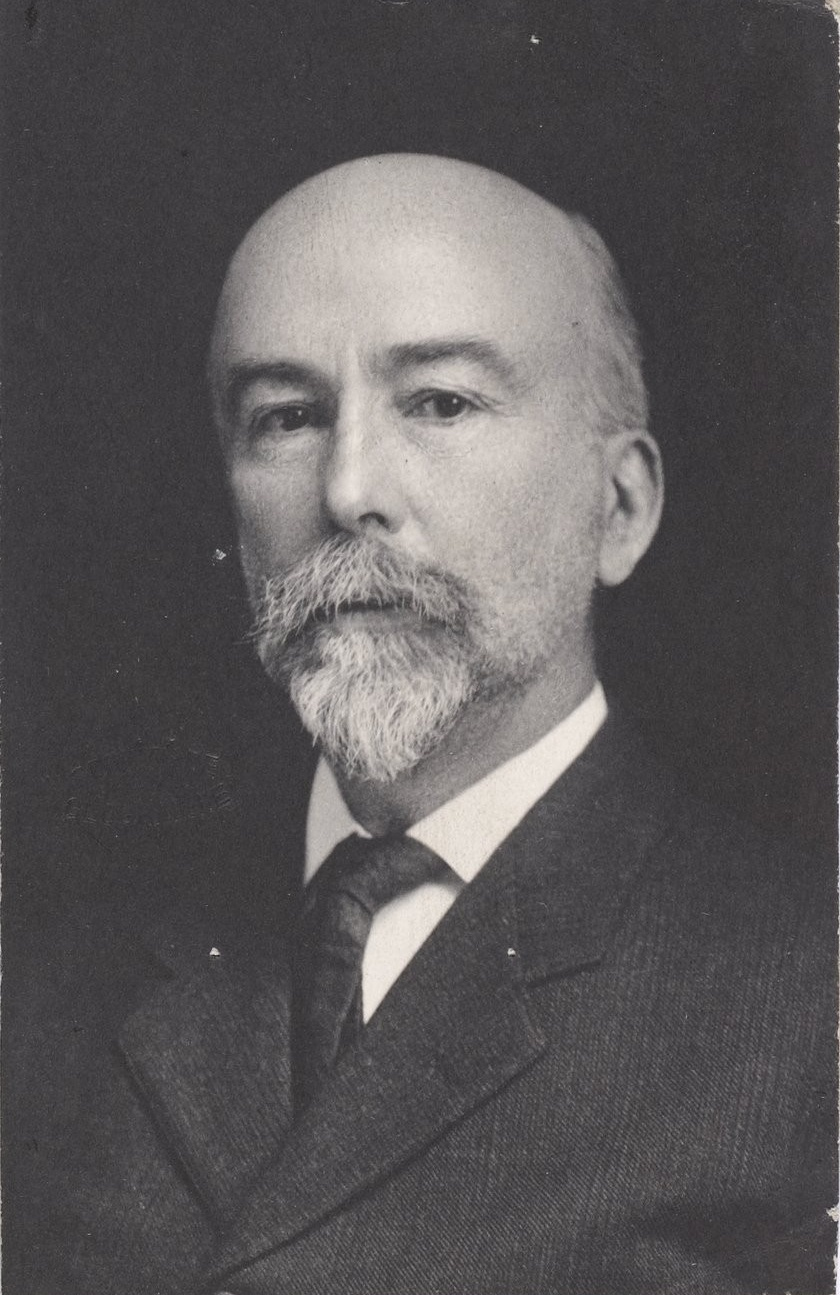
\includegraphics[width=0.7\linewidth]{obrazky/uvod/davies}
	\caption{William Morris Davies (zdroj: Bibliothèque nationale de France https://gallica.bnf.fr/ark:/12148/btv1b8453640z, volné dílo)}
	\label{fig:davies}
\end{figure}

Proti představám W. M. Davise vystupoval Walther Penck. Odmítal představu, že po rychlém výzdvihu může být dlouhé stabilní období pro vývoj následných forem reliéfu. Dle Pencka je podoba krajiny závislá na tom, zda výzdvih se zvětšuje, snižuje nebo je konstantní v průběhu času.
Obecně můžeme říct, že v počátcích byla evropská goemorfologie do velké míry popisná a klasifikační, kdežto americká byla vysvětlující -- interpretační.

Od konce 40. ket dochází zejména v USA a UK k rozvoji kvantitativní geomorfologie. Průkopníkem je R.E. Horton, který v roce 1945 publikoval práci o hydrologii povodí. Následující roky se tak rozvíjela geomorfometrie a intenzivně se měřily geomorfologické procesy v terénu. V kontinentální Evropě se během té doby intenzivněji rozvíjela klimatická geomorfologie.

Během 60. a 70. let se geomorfologie v UK a USA přeorientovala na tvorbu prediktivních modelů k předpovídání krátkodobých změn reliéfu. Postupně narůstala globalizace geomorfologie až do současné podoby.
%\section{Česká a československá geomorfologie}
%\todo[inline]{dopsat}

\section{Geomorfologické disciplíny}
Geomorfologii můžeme rozdělit podrobněji podle předmětu studia do několika disciplín.
\begin{enumerate}
	\item \emph{Strukturní geomorfologie} se zabývá vlivem geologické struktury na tvary zemského povrchu.
	\item \emph{Klimatická geomorfologie} studuje vliv klimatu na vývoj reliéfu.
	\item \emph{Dynamická geomorfologie} zkoumá geomorfologické procesy.
	\item \emph{Paleogeomorfologie} nebo také historická geomorfologie se zabývá výzkumem georeliéfu minulých geologických období.
	\item \emph{Antropogenní geomorfologie} studuje tvary reliéfu, které člověk vytváří a procesy, které způsobují jejich vznika a vývoj. Také sleduje jak člověk ovlivňuje přírodní morfogenetické procesy.
	\item \emph{Aplikovaná geomorfologie} neboli užitá geomorfologie aplikuje geomorfologické poznatky a přístupy pro řešení celé řady socioekonomických problémů.
\end{enumerate}

	
	\chapter{Základní koncepty}
	\section{Proces a forma}
Ústředním tématem geomorfologie je zkoumání interakcí mezi geomorfologickými procesy a formami reliéfu. Procesy utvářejí georeliéf a naopak georeliéf ovlivňuje geomorfologické procesy. Podívejme se na řeku v horách. Velký sklon říčního koryta (forma) jí dává velkou energii. Řeka tak má poměrně velkou schopnost eroze a transportu materiálu (procesy). V místě zaústění toku do nížin sklon koryta klesá (změna formy) a erozní a transportní schopnost řeky se také snižuje, což způsobuje naopak akumulaci materiálu v předpolí (procesy).

Z forem reliéfu můžeme vyčíst celou řadu informací o procesech, které je utvářely nebo utvářejí. Například z tvaru písečných dun lze zjistit jakého směru vanou převládající větry; charakter říčního koryta nám může napovědět o hydrologickém režimu řeky, kolik a jaké sedimenty unáší a podobně. 

Mnohé formy reliéfu jsou reliktem geomorfologických procesů dob minulých. Díky nim tak můžeme studovat historii a vývoj krajiny. Příkladem mohou být ledovcová údolí, kary a morény ve Vysokých Tatrách -- důkaz přítomnosti ledovců v pleistocénu.

\section{Endogenní a exogenní procesy}
jak již bylo zmíněno, reliéf se vyvíjí působením \emph{geomorfologických procesů}. Tyto procesy dělíme do dvou základních skupin, a to na endogenní a exogenní. \textbf{Endogenní} procesy mají svůj původ v zemském nitru. Jejich hlavní zdroj energie je rozpad radioaktivních prvků v zemském jádře. Projev endogenních procesů je například vulkanismus, zemětřesení, pohyby litosférických desek. \textbf{Exogenní} procesy mají svůj zdroj energie ve Slunci. Uplatňuje se u nich ale i gravitace, zemská rotace a slapové jevy. 

Ve své základní podstatě je georeliéf výsledkem protichůdných působení endogenních a exogenních procesů. Obecně můžeme říct, že endogenní procesy hlavně budují reliéf do výšky (Obr. \ref{fig:zmenyvysky}). Jejich působením vznikají pohoří, sopky a podobně. Zvyšují tak vertikální členitost reliéfu. Vyčleňují se tři  hlavní skupiny endogenních procesů. \emph{Magmatické procesy} zahrnují přesuny roztavených hornin (magmatu) k zemskému povrchu. \emph{Orogeneze} označuje vznik rozsáhlých pásemných pohoří. \emph{Epeirogeneze} je výzdvih velkých území bez zjevného vrásnění či rozlámání hornin. 

Exogenní procesy naopak snižují a zarovnávají zemský reliéf (Obr. \ref{fig:zmenyvysky}). Souhrnně se tomuto procesu říká \emph{denudace}. Denudace zahrnuje jak odnos pevných částic, což je nazýváno jako \emph{eroze}, tak i rozpuštěných látek (\emph{chemická denudace}). Samozřejmě i exogenní procesy mohou lokalizovaně zvyšovat zemský reliéf (např. písečné duny, morény).

\begin{figure}[h]
	\centering
	\includegraphics[width=1\linewidth]{obrazky/uvod/zmeny_vysky}
	\caption{Schéma znázorňující změny v nadmořské výšce způsobené různými exogenními a endogenními procesy. Plusové znaménko znamená nárůst nadmořské výšky a potenciální energie, mínus značí opak. Upraveno podle \textcite{summerfieldGlobalGeomorphologyIntroduction1999}}
	\label{fig:zmenyvysky}
\end{figure}

%\section{Geomorfologický systém}
%\todo[inline]{geomorfologický systém}
%%\begin{myboxgreen}
%%	test boxu
%%\end{myboxgreen}

\section{Měřítko}
\subsection{Prostorové měřítko}
Georeliéf lze studovat v různém \emph{prostorovém měřítku}. V planetárním či kontinentálním měřítku studujeme například celé orogény (např. Andy, Himaláje), rychlost jejich výzdvihu, intenzitu denudačních procesů a vliv klimatu na ně. Při bližším pohledu se dostáváme na regionální (makro) měřítko. Jedná se zpravidla o území s jednotnou geologickou stavbou. Dalším příblížením se zaměřujeme již na dílčí formy reliéfu. Studujeme malá povodí, jednotlivé meandry, písečné duny. Ve větším detailu (mikro měřítko) pak studujeme drobné tvary reliéfu -- štěrkové lavice, zlomový sráz vzniklý jedním zemětřesením, mělké sesuvy. Lze se ale přiblížit ještě více. V největším detailu pak můžeme studovat mikroreliéf např. skalních stěn (příkladem drobných tvarů jsou voštiny). 

Je třeba mít na paměti, že pro každou úroveň prostorového měřítka se uplatňují odlišné metody. Při studiu velkých území využijeme např. dálkový průzkum Země, práci v geografických informačních systémech. Při mikro měřítku se bude výzkum odehrávat ve větší míře na daném místě v terénu. Budeme např. zkoumat odkryvy a odebírat vzorky, které následně zpracujeme v laboratoři za účelem zjištění jejich zrnitosti, obsahu organické hmoty apod.

%\begin{table*}[h]
%	\setlength{\tabcolsep}{0.5pt}
%	\footnotesize
%	\begin{tabularx}{1\textwidth}{@{}llllllllllX@{}}
%		\toprule
%		\multirow{3}{*}{\begin{tabular}[c]{@{}l@{}}Prostorové \\ měřítko\end{tabular}} &
%		\multicolumn{2}{c}{Rozměry} &
%		\multicolumn{4}{c}{Příklady tvarů} &
%		\multicolumn{2}{c}{Hlavní kontrolní faktory} &
%		\multicolumn{2}{c}{\multirow{3}{*}{Časové měřítko}} \\ \cmidrule(lr){2-3} \cmidrule(lr){4-7} \cmidrule(lr){8-9}
%		\multicolumn{1}{c}{} &
%		\multicolumn{1}{c}{\multirow{2}{*}{Lineární}} &
%		\multicolumn{1}{c}{\multirow{2}{*}{Plošné}} &
%		\multicolumn{1}{c}{Endogenní} &
%		\multicolumn{3}{c}{Exogenní} &
%		\multicolumn{1}{c}{\multirow{2}{*}{Endogenní}} &
%		\multicolumn{1}{c}{\multirow{2}{*}{Exogenní}} &
%		\multicolumn{2}{c}{} \\ \cmidrule(lr){5-7} 
%		\multicolumn{1}{c}{} &
%		\multicolumn{1}{c}{} &
%		\multicolumn{1}{c}{} &
%		&
%		\multicolumn{1}{c}{Fluviální} &
%		\multicolumn{1}{c}{Glaciální} &
%		\multicolumn{1}{c}{Eolické} &
%		\multicolumn{1}{c}{} &
%		\multicolumn{1}{c}{} &
%		\multicolumn{2}{c}{} \\ \midrule
%		Mikro &
%		$<0,5$ &
%		$<0,25$ &
%		Malé zlomové svahy &
%		Tůně a peřeje v malém povodí &
%		Malé morénové hřbety &
%		Písečné čeřiny &
%		Jednotlivá zemětřesení nebo sopečné erupce &
%		Mikroklima, meteorologické události &
%		Steady tim &
%		$10^1$ \\ \midrule
%		Meso &
%		$0,5$--$10$ &
%		$0,25$--$10^2$ &
%		Malé sopky &
%		Malá ledovcová údolí &
%		Meandry &
%		Duny &
%		Místní a regionální isostatický výzdvih, lokální vulkanismus a zemětřesení &
%		Lokální klima, krátkodobé změny klimatu &
%		dynamický čas &
%		$10^3$ \\ \midrule
%		Macro &
%		$10$--$10^3$ &
%		$10^2$--$10^6$&
%		Zlomová pohoří  & %Block-faulted terrain
%		Nivy velkých řek &
%		Ledovcové čapky &
%		Písečná moře &
%		Regionální výzdvih a pokles &
%		Regionální klima, dlouhodobé změny klimatu (střídání glaciálů a interglaciálů) &
%		\multirow{2}{*}[-2em]{Cyklický čas} &
%		\multirow{2}{*}{$10^7$} \\ \cmidrule(lr){1-9}
%		Mega &
%		$>10^3$ &
%		$>10^6$ &
%		Hlavní orogény &
%		Hlavní povodí &
%		Kontinentální ledovcové příkrovy &
%		Rozsáhlá písečná moře &
%		Dlouhodobé rozložení výzdvihu, poklesu a pohyby litosférických desek &
%		Hlavní klimatické zóny, dlouhotrvající změny klimatu (doby ledové) &
%		&
%		\\ \bottomrule
%	\end{tabularx}
%	\caption{Hierarchie prostorových a časových měřítek (upraveno podle \textcite{summerfieldGlobalGeomorphologyIntroduction1999})}
%	\label{tab:meritko}
%	
%\end{table*}

\subsection{Časové měřítko}
Vývoj georeliéfu probíhá i v rozličném čase. Některé změny se odehrávají během vteřin, jiné zase trvají milióny let. Zlomový sráz může vzniknout během okamžiku při zemětřesení. Může ale trvat stovky let i tisíce let, než jej eroze zcela zahladí. Rychlost, jakou bude vzniklý stupeň zahlazen závisí na celé řadě faktorů. První faktor ovlivňující životnost tvaru je to, zda prostředí, ve kterém se nachází je charakteristické vysokou mírou eroze a akumulace nebo je to naopak relativně klidné prostředí. V prvním případě může být stupeň zhlazen během několika málo desítek let. V druhém případě bude patrný v reliéfu i po několika staletích. Druhý faktor je odolnost materiálu, ze kterého je tvořen tvar vůči odnosu. Vodní tok v sedimentech bude snáz proměňovat své koryto, než kdyby tekl ve skalním korytě. Třetím faktorem je velikost tvaru. Menší tvary vznikají a zanikají rychleji, než tvary velké. 

\section{Základní teoretická východiska}

\subsection{Zachování hmoty v krajině}
Zemský povrch, georeliéf je dynamickým systémem, skrz který dochází k přesunům hmoty. Hmota nikde nemizí, jen je přemisťována z jednoho místa na druhé. Když se sesune část svahu, dojde k přesunu hmoty z horní části svahu k jeho úpatí. V odlučné oblasti materiál chybí, v akumulační zóně naopak hmoty přibylo. Pro určitou část zemského povrchu za určitou dobu platí: 
\begin{equation}\label{key}
	I-O=\delta ST	
\end{equation}
\begin{eqexpl}
	\item{$I$}vstup hmoty (to co přibylo)
	\item{$O$}výstup hmoty (to co ubylo)
	\item{$\delta ST$}změna zásob hmoty
\end{eqexpl}

Velikost a charakter změny zásob hmoty v určitém území určuje její charakter. Hory, které erodují rychleji než je tektonický výzdvih se snižují. Pokud se do řeky dostává více sedimentů, než je schopna unášet, tak se časem koryto zaplní \parencite{biermanKeyConceptsGeomorphology2014}.

\subsection{Zachování energie}
Energii nelze vyrobit ani zničit, ale pouze přeměnit na jiný druh energie. Potenciální energie daná pozicí v reliéfu se může změnit na kinetickou energii. Když se na svahu uvolní kámen, začne se kutálet dolů. Jeho potenciální energie daná jeho pozicí na svahu se mění v kinetickou energii. Část kinetické energie se mění na teplo z důvodu tření. 

\subsection{Pohyb hmoty}
Pohyb hmoty je od zdrojnice (angl. source) materiálu k místu akumulace (angl. sink). Většinou se jedná o jednosměrný tok z vyšších poloh do nižších. Materiál je unášen řekou z horních částí toku až do sedimentačních pánví (jezero, moře)

\subsection{Rovnováha sil a prahy}
Systém je udržován v dynamické rovnováze celou řadou zpětných vazeb. Narušením systému může dojít k takovému vychýlení, že se již není schopen vrátit zpět na stejnou trajektorii vývoje. Po dílčím období nestability dochází k nastolení nové dynamické rovnováhy a systém se vyvíjí po nové trajektorii.

\begin{figure*}[h]
	\centering
	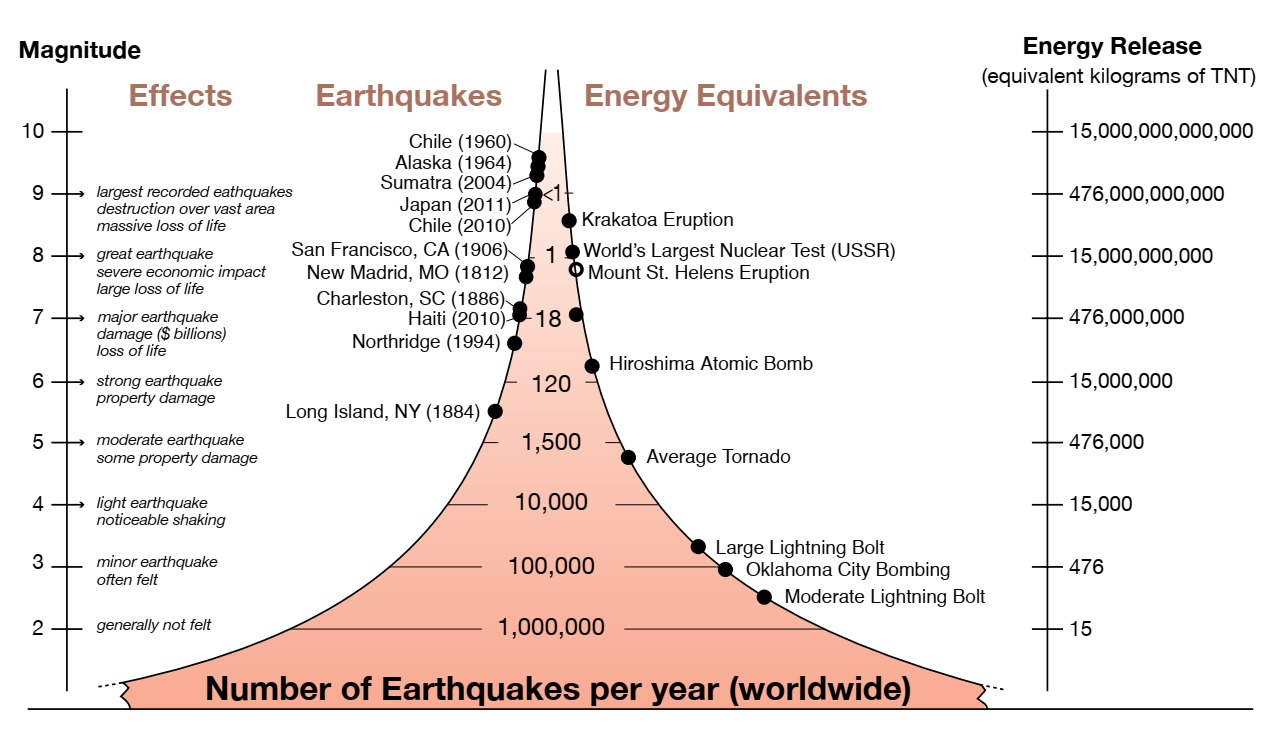
\includegraphics[width=1\linewidth]{obrazky/uvod/frekvence}
	\caption{Četnost zemětřesení (zdroj: IRIS.edu)}
	\label{fig:frekvence}
\end{figure*}

\subsection{Magnitudo a frekvence geomorfologických procesů}
Jevy malého magnituda (rozsahu, intezity...) se dějí často, mají tedy vysokou frekvenci opakování. Příkladem jsou zemětřesení. Slabá zemětřesení (magnitudo 3 a méně) jsou četná (Obr. \ref{fig:frekvence}). Ročně se jich vyskytne $> 1000000$. Silná zemětřesení (magnitudo $>=7$) se vyskytují jen v počtu cca 20 za rok, z k těm nejsilnějším dochází jen jednou za několik let. 
Události malého magnituda nemají zpravidla velký geomorfologický účinek. Naopak jevy velkého magnituda způsobují velké změny v reliéfu, postihují rozsáhlé oblasti apod. Opravdu silných zemětřesení se ročně vyskytne jen pár, ale mají dalekosáhlé důsledky jak pro společnost, tak pro georeliéf.




	%%%%%%%%%%%%%%%%%%%%%%
	\part{Endogenní procesy a formy reliéfu}
	
	\chapter{Stavba Země a globální strukturní geomorfologie}
	\section{Stavba Země}

\subsection{Zemský plášť a kůra}
Země se sestává ze tří hlavních částí: \textbf{zemského jádra}, \textbf{pláště} a \textbf{kůry} (Obr. \ref{fig:stavba_zeme}). Hranice mezi jednotlivými částmi byly zjištěné studiem průchodu zemětřesných vln zemským tělesem. Na těchto hranicích se totiž výrazně mění chování zemětřesných vln či skrz hranici nemohou prostupovat. Rozhraní mezi zemskou kůrou a pláštěm tvoří Mohorovičičova diskontinuita (zkráceně Moho). Pod kontinenty se nachází v průměrné hloubce 35 km, pod oceány v pouhých 5--10 km pod oceánským dnem. Zemská kůra tedy nemá všude stejnou tloušťku. Mocnost \textbf{Oceánské kůry} je 5--10 km. Skládá se hlavně z bazaltové a tenké sedimentární vrstvy. \textbf{Kontinentální kůra} je daleko mocnější, v průměru má okolo 35 km avšak pod některými pohořími může dosahovat i 70 km. 

%
%\begin{myboxgreen}
%	Obrázek o stavbě Země máme díky sledování průběhu zemětřesných vln zemským tělesem.
%\end{myboxgreen}

\begin{figure*}[h]
	\includegraphics[width = \textwidth]{./tectonic/Earth_cutaway_schematic-en.pdf}
	\caption{Průřez Zemí (není v měřítku) (zdroj: USGS, volné dílo, via Wikimedia Commons)}
	\label{fig:stavba_zeme}
\end{figure*}

\subsection{Teorie deskové tektoniky}
Procesy, které ovlivňují reliéf v globálním měřítku se odehrávají v \textbf{litosféře} neboli pevném obalu Země. Litosféra je tvořena rigidními, neroztavenými horninami a zahrnuje zemskou kůru, tak i svrchní, pevnou část zemského pláště. Podle typu zemské kůry tak rozlišujeme i litosféru na oceánskou a kontinentální. 
Pod litosférou se nachází \textbf{astenosféra}. Jedná se o zónu částečně natavených hornin, což způsobuje, že se astenosféra chová plasticky. 
Litosféra není celistvá. Ve skutečnosti je rozčleněna do \textbf{litosférických desek}, které se nezávisle na sobě pohybují, kloužou, po astenosféře. Existuje 7 hlavních, celá řada menších litosférických desek. Mezi ty hlavní patří Euroasijská, Pacifická, Severoamerická, Jihoamerická, Africká, Indo-australská a Antarktická. Z menších desek jsou nejznámější např. Nazca, Kokosová, Filipínská, Arabská. 

\begin{figure*}[h]
	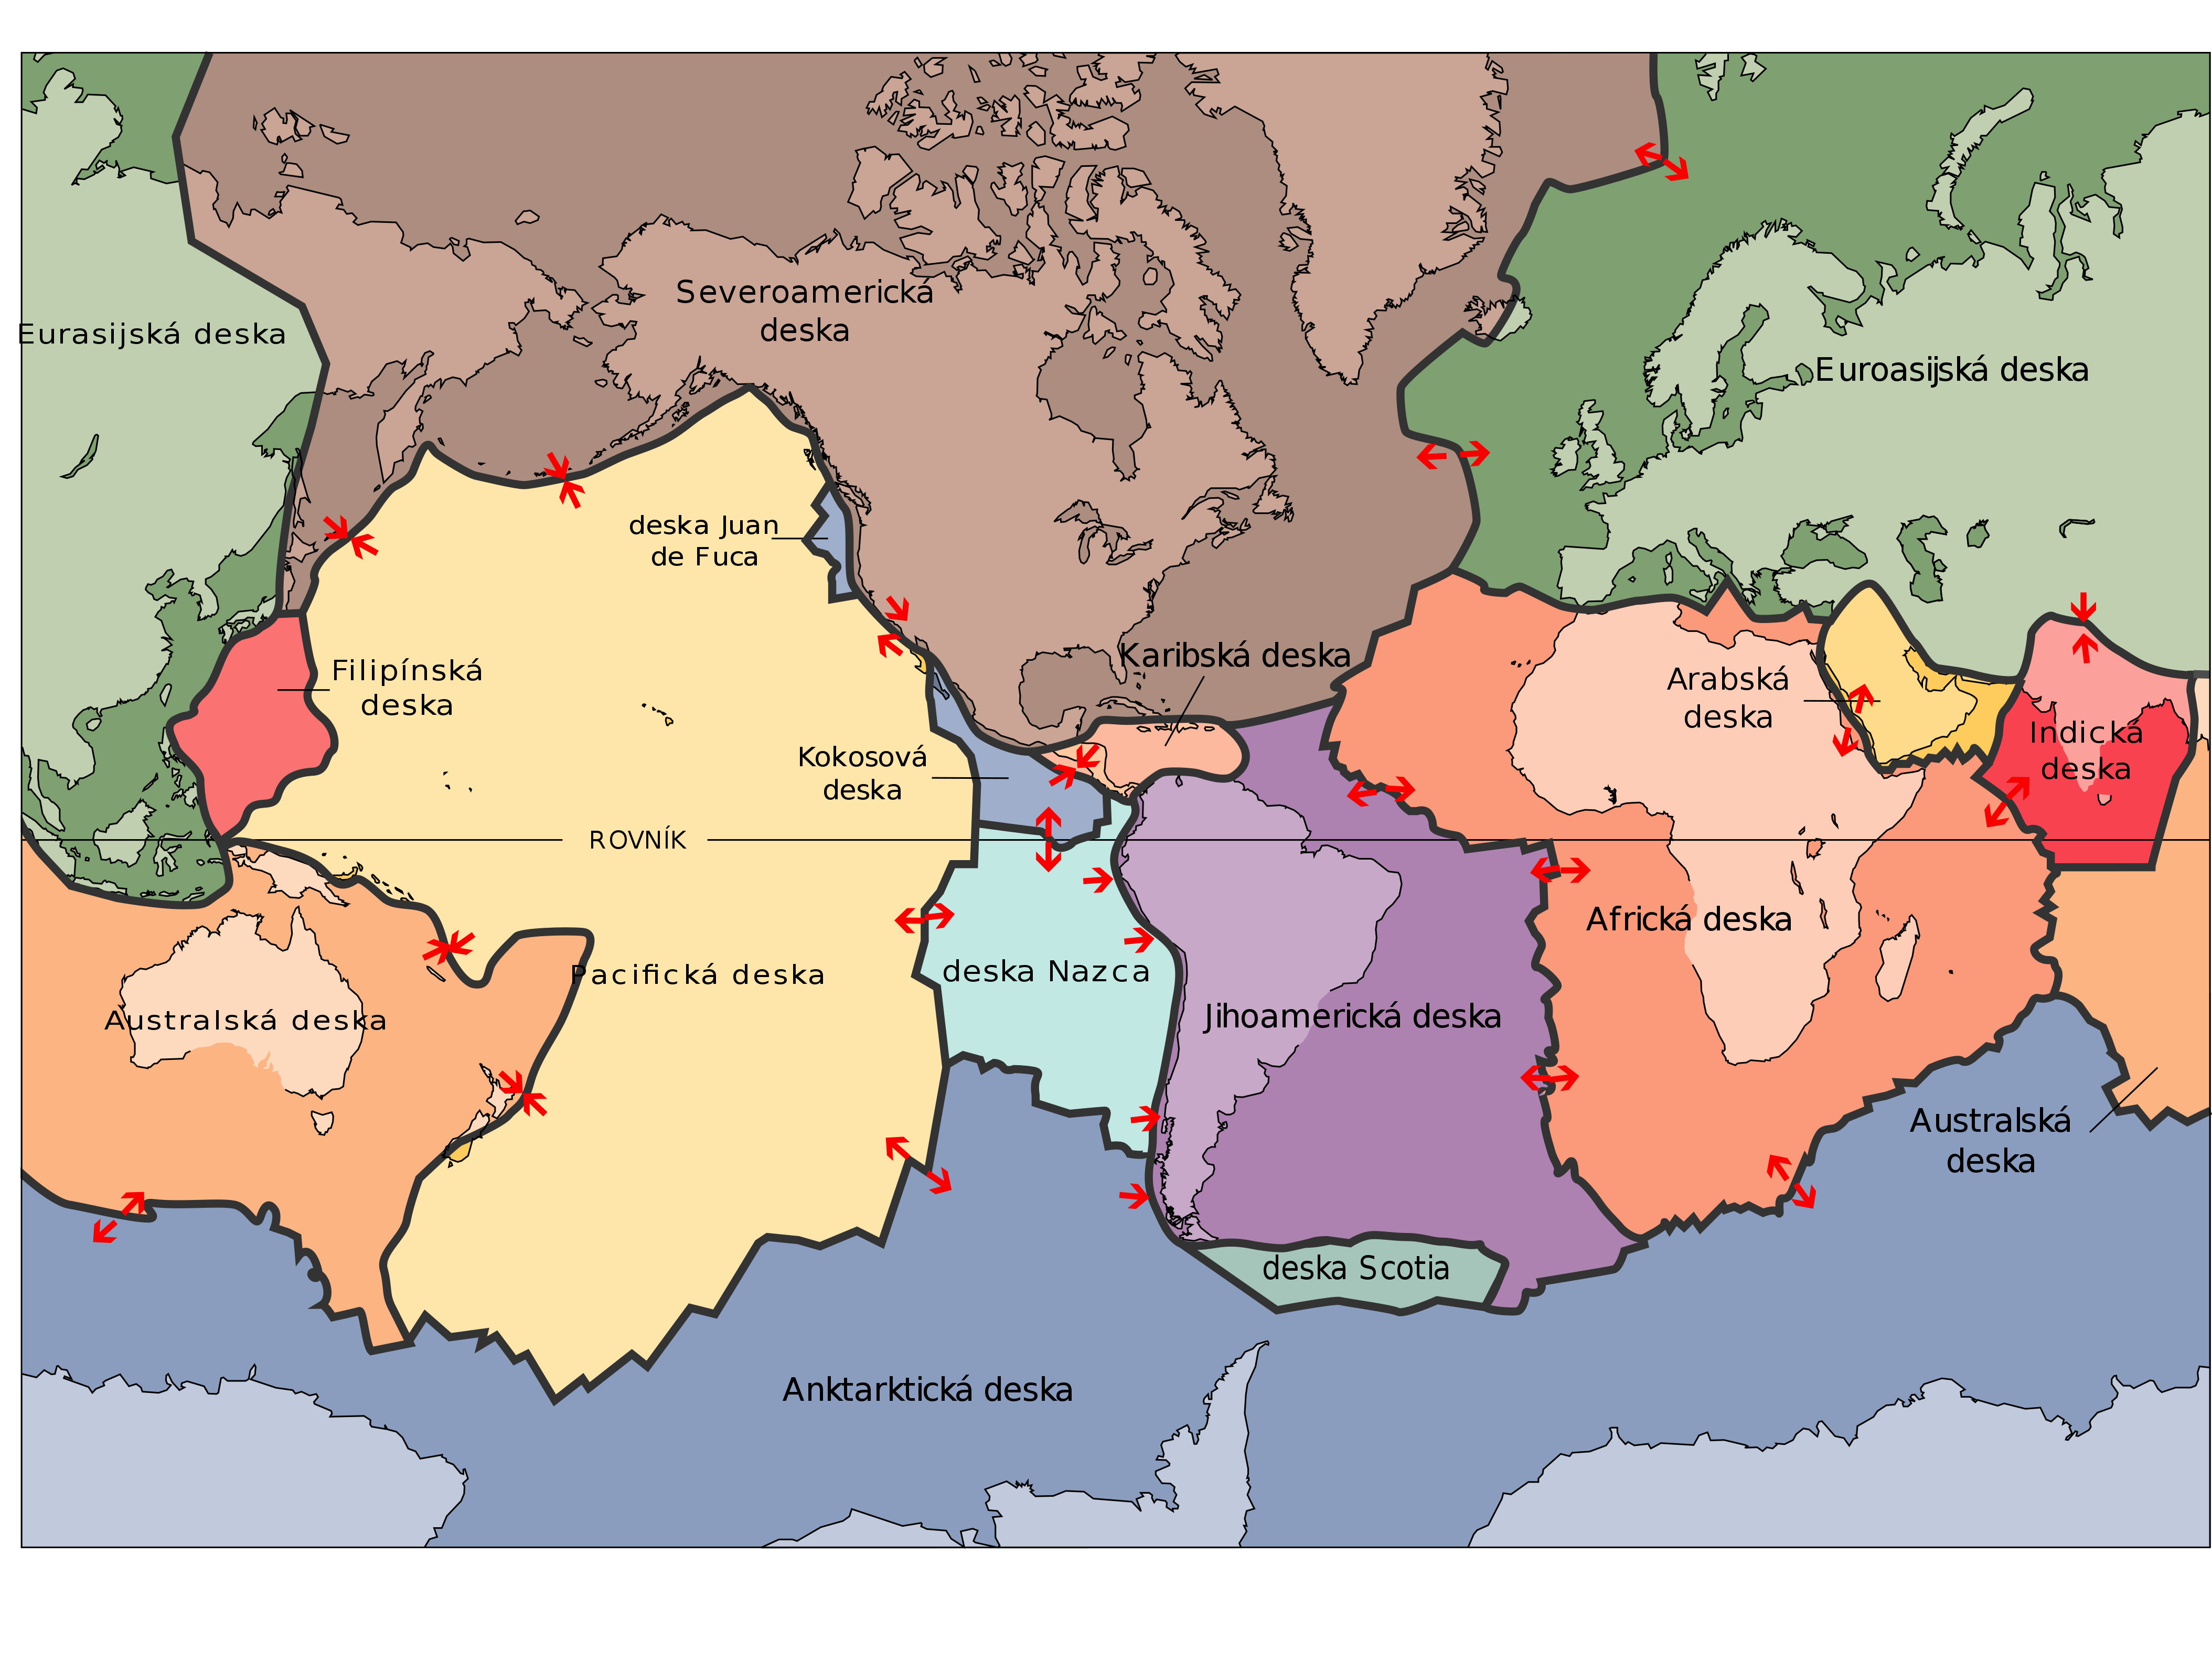
\includegraphics[width=\textwidth]{./tectonic/Plates_tect_cs.svg}
	\caption{Hlavní tektonické desky (zdroj: Jklamo, volné dílo, via Wikimedia Commons}
\end{figure*}

\subsubsection{Okraje litosférických desek}
Existují celkem tři typy rozhraní litosférických desek, a to divergentní, konvergentní a transformní. \textbf{Divergentní} rozhraní jsou takové, kde se litosférické desky od sebe vzdalují. Typickou ukázkou divergentního rozhraní jsou středooceánské hřbety jako je např. Středoatlantský hřbet. Na středooceánských hřbetech vzniká nová oceánská kůra, rozšiřuje se tak oceánské dno. Stáří oceánské kůry roste na obě strany od osy hřbetu. Středooceánské hřbety jsou rozčleněny transformními zlomy, které způsobují jejich klikatění v půdorysu. 

Při pohybu litosférických desek proti sobě hovoříme o \textbf{konvergentním} okraji. Pokud se střetávají dvě oceánské desky, jedna se podsouvá pod druhou neboli dochází k \textbf{subdukci}. V místě subdukce vzniká hlubokoceánský příkop a vulkanický ostrovní oblouk.  Subdukce oceánské litosféry pod kontinentální je opět charakteristické hlubokooceánským příkopem a dochází k orogenezi s aktivním vulkanismem. Typickým příkladem je podsouvání desky Nazca pod Jihoamerickou desku. Kde takto vznikly Andy. Při střetu dvou pevninských desek nedochází k podsouvání jedné pod druhou, nýbrž dochází k intenzivní orogenezi. 

Třetím typem je \textbf{transformní okraj} někdy také \textbf{konzervační okraj}. V tomto případě se litosférické desky horizontálně podél rozhraní. Typickým příkladem transformního okraje je zlom San Andreas.

V případě, že se okraj kontinentu shoduje s okrajem litosférické desky nazýváme ho \textbf{aktivním okrajem}. Typickým příkladem je západní okraj Jižní Ameriky. Pokud je okraj kontinentu uvnitř litosférické desky jedná se o \emph{pasivní okraj} kontinentu. 
% TODO: \usepackage{graphicx} required
\begin{figure*}[h]
	\centering
	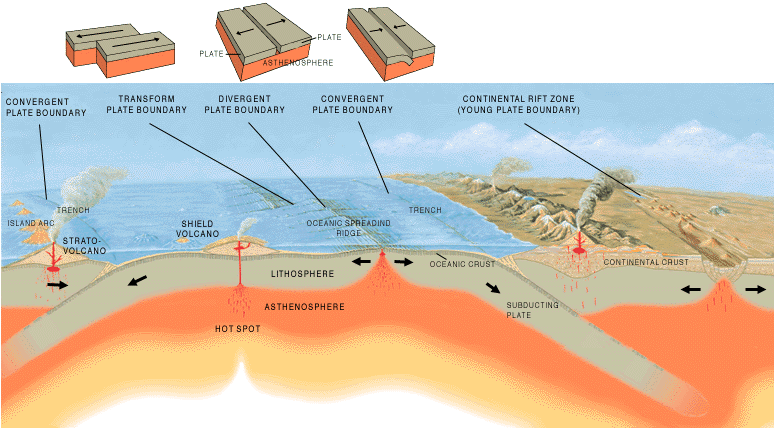
\includegraphics[width=1\linewidth]{obrazky/tectonic/Tectonic_plate_boundaries}
	\caption{Okraje litosférických desek (Autor: Jose F. Vigil. USGS, volné dílo, via Wikimedia Commons)}
	\label{fig:tectonicplateboundaries}
\end{figure*}


\begin{table*}[]
	\begin{tabularx}{1\textwidth}{XXXXXX}
		\toprule
		&          & \multicolumn{3}{c}{Morfologické a strukturní prvky}                                                                   \\ \midrule
		Typ rozhraní &
		Napěťový režim &
		Oceánská--oceánská litosféra &
		Oceánská--kontinentální litosféra &
		Kontinentální--kontinentální litosféra \\ \midrule
		Divergentní & Extenzní & Středooceánský hřbet, vulkanická aktivita & --                          & Riftová údolí, vulkanismus                  \\ \midrule
		\multirow{2}{*}{Konvergentní} &
		\multirow{2}{*}{Kompresní} &
		Oceánský příkop a vulkanický ostrovní oblouk &
		Oceánský příkop, pásemná pohoří na okrajích kontinenů a vulkanismus &
		-- \\
		&          & Komplexní kolizní zóna ostrovních oblouků & Modifikovaná pásemná pohoří & Pásemná pohoří, omezená vulkanická aktivita \\ \midrule
		Transformní & Střižný  & Hřbety a údolí                            & --                          & Zlomová zóna, bez vulkanismu               \\ \bottomrule
	\end{tabularx}
	\caption{Klasifikace a hlavní charakteristiky rozhraní litosférických desek}
	\label{tab:my-table}
\end{table*}

Okraje litosférických desek jsou důležitým místem, kde se odehrává celá řada geodynamických procesů. Jsou to místa, kde je soustředěná vulkanická a zemětřesná činnost (Obr. \ref{fig:zemetresenidesky}). 

\begin{figure*}[h]
	\centering
	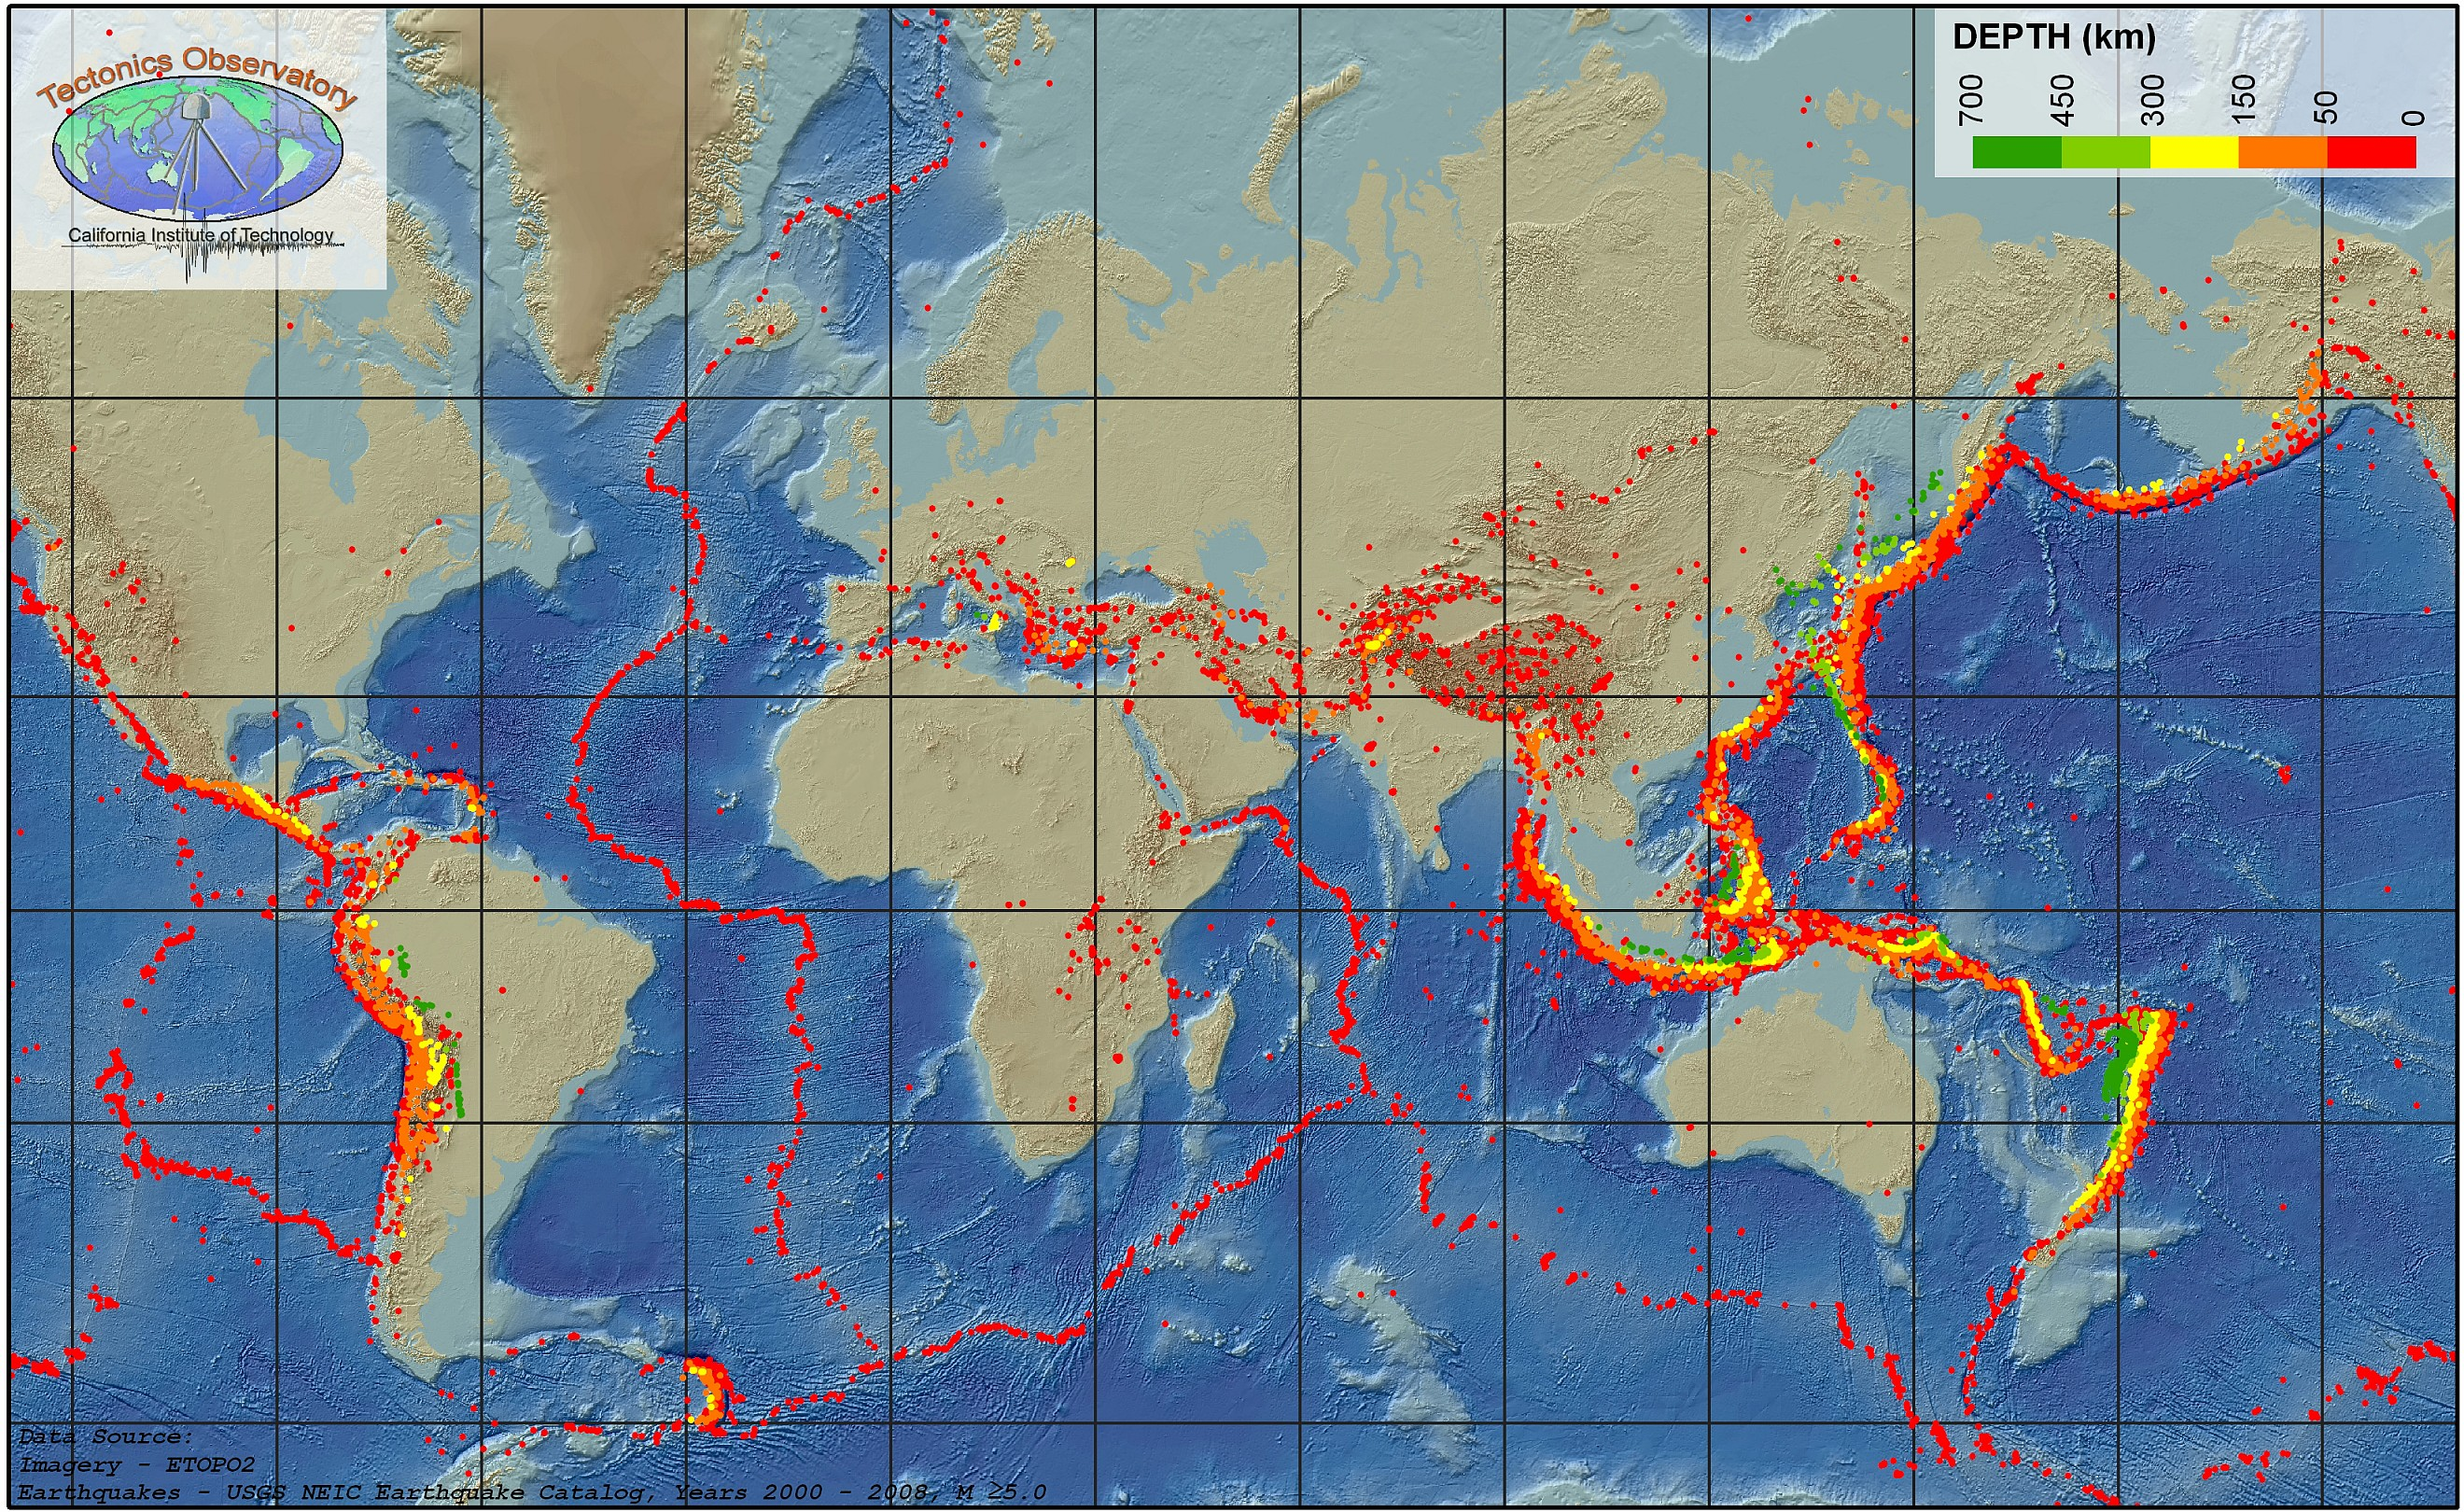
\includegraphics[width=1\linewidth]{obrazky/tectonic/global_seismicity_h}
	\caption{Mapa zemětřesení o magnitudu $>=5$ve světě mezi roky 2000--2008 (Zdroj: Lisa Christiansen, Caltech Tectonics Observatory, \url{https://www.nsf.gov/news/mmg/mmg_disp.jsp?med_id=64691})}
	\label{fig:zemetresenidesky}
\end{figure*}

\subsubsection{Příčiny pohybu litosférických desek}
Příčiny pohybu litosférických desek jsou stále předmětem vědeckého bádání. Je několik mechanismů, kterými je pohyb vysvětlován. Tím hlavním je přítomnost konvekčních proudů v zemském plášti. Tyto proudy vystupují pod středooceánskými hřbety, kde se vychylují do strana klesají v místech subdukčních zón. Boční pohyb proudů v plášti tak unáší litosférické desky. Další mechanismem je gravitační skluz litosféry. Směrem od středooceánských hřbetů roste její mocnost, což díky gravitaci způsobuje její klouzání směrem k subdukčním zónám. Pohyb strhává astenosféru v přímém kontaktu s litsoférickou deskou, což má za následek výstup kompenzačních proudů v místě středooceánských hřbetů. Jako možný mechanismus se uvádí i odtlačování litosférických desek lávou vystupijící na povrch v místě středooceánských hřbetů. Jako důležitý mechanismus se ukazuje ponořování oceánské litosféry do astenosféry v zónách subdukce. Stará oceánská litosféra má vyšší hustotu než astenosféra. Část litosférické desky, která se noří do astenosféry až do hloubky cca \SI{700}{\kilo\metre}, tak stahuje její zbylou část sebou. Jelikož mezi litosférou a astenosférou je velký teplotní rozdíl (v hloubce \SI{400}{\kilo\metre} může být litosférická deska až o \SI{1000}{\degreeCelsius} chladnější oproti okolnímu plášti) a litosféra špatně vede teplo, tak vyrovnávání teplot hustoty trvá dlouhou dobu. Pozorování rychlosti pohybu litosférických desek podporuje tento mechanismus. Desky, které mají dlouhé subdukční zóny (jako je např. Pacifická) se pohybují rychleji (\SIrange{60}{90}{\milli\metre\per\rok}) než desky, které nemají tak rozsáhle subdukční zóny (rychlost pod \SI{40}{\milli\metre\per\rok}).

\subsection{Izostáze}
Zjednodušeně lze říct, že litosféra plave na astenosféře podobně jako plave kus dřeva nebo ledová kra na vodní hladině. Aby litosféra dosáhla hydrostatické rovnováhy vzhledem ke své hustotě a tloušťce, dochází u ní k vertikálním pohybům. Pro tento stav rovnováhy byl zaveden právě termín \textbf{izostáze}. Existují dva modely izostáze. \textbf{Prattův model} je založen na rozdílné hustotě různých částí litosféry. To znamená, že jedna sekce litosféry bude výš, než druhá díky své nižší hustotě. \textbf{Airyho model} zase pojednává o rozdílných tloušťkách jednotlivých sekcí litosféry o stejné hustotě. Oba modely se ale mohou kombinovat. Kontinentální litosféra je výš než oceánská, protože má nižší hustotu a zároveň větší mocnost. Výškové rozdíly v rámci kontinentů jsou spojené s rozdíly v mocnosti kontinentální kůry. Vysoká pohoří mají hluboké kořeny z hornin o menší hustotě.
% TODO: \usepackage{graphicx} required
\begin{figure*}[h]
	\centering
	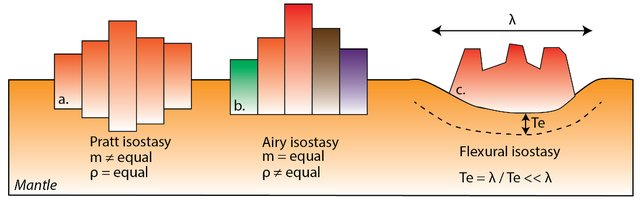
\includegraphics[width=1\linewidth]{obrazky/tectonic/isostasy}
	\caption{Tři typy izostáze. A) Prattův model izostáze b) Airyho model c) Flexurní izostáze způsobena zatížením litosféry např. ledovcem -- glaciizostáze. (Zdroj: \textcite{beniestContinentalRiftingConjugate2017})}
	\label{fig:isostasy}
\end{figure*}

Zvláštním typem izostáze je tzv. \emph{glaciisostáze}. Ledovce během glaciálu svou vahou způsobily prohnutí zemské kůry, což vedlo ke kompenzačnímu výzdvihu v okolí kontinentálních ledovců. Důsledkem zániku ledovc je návrat zemské kůry do rovnovážné polohy. V místech, kde zemská kůra byla zatlačena dochází ke \emph{glaciisostatickému výydvihu} (\textit{glaciisostatic rebound}) a naopak k poklesům, kde byla předtím vzydvižena.
\subsection{Horké skvrny}
Horké skvrny (\textit{hot spots}) jsou specifická místa v zemském tělese, kde je zvýšený tok geotermální energie a magma se dostává k povrchu. Z toho pak pramení vulkanická činnost. Tyto vulkanické oblasti nekopírují okraje litosférických desek. Jelikož horké skvrny se nepohubují vzniká v důsledku pohybu litosférických desek řetězce sopečných ostrovů. Klasickým příkladem je Havajské souostroví (Obr. \ref{fig:hawaiihotspot}.

% TODO: \usepackage{graphicx} required
\begin{figure*}
	\centering
	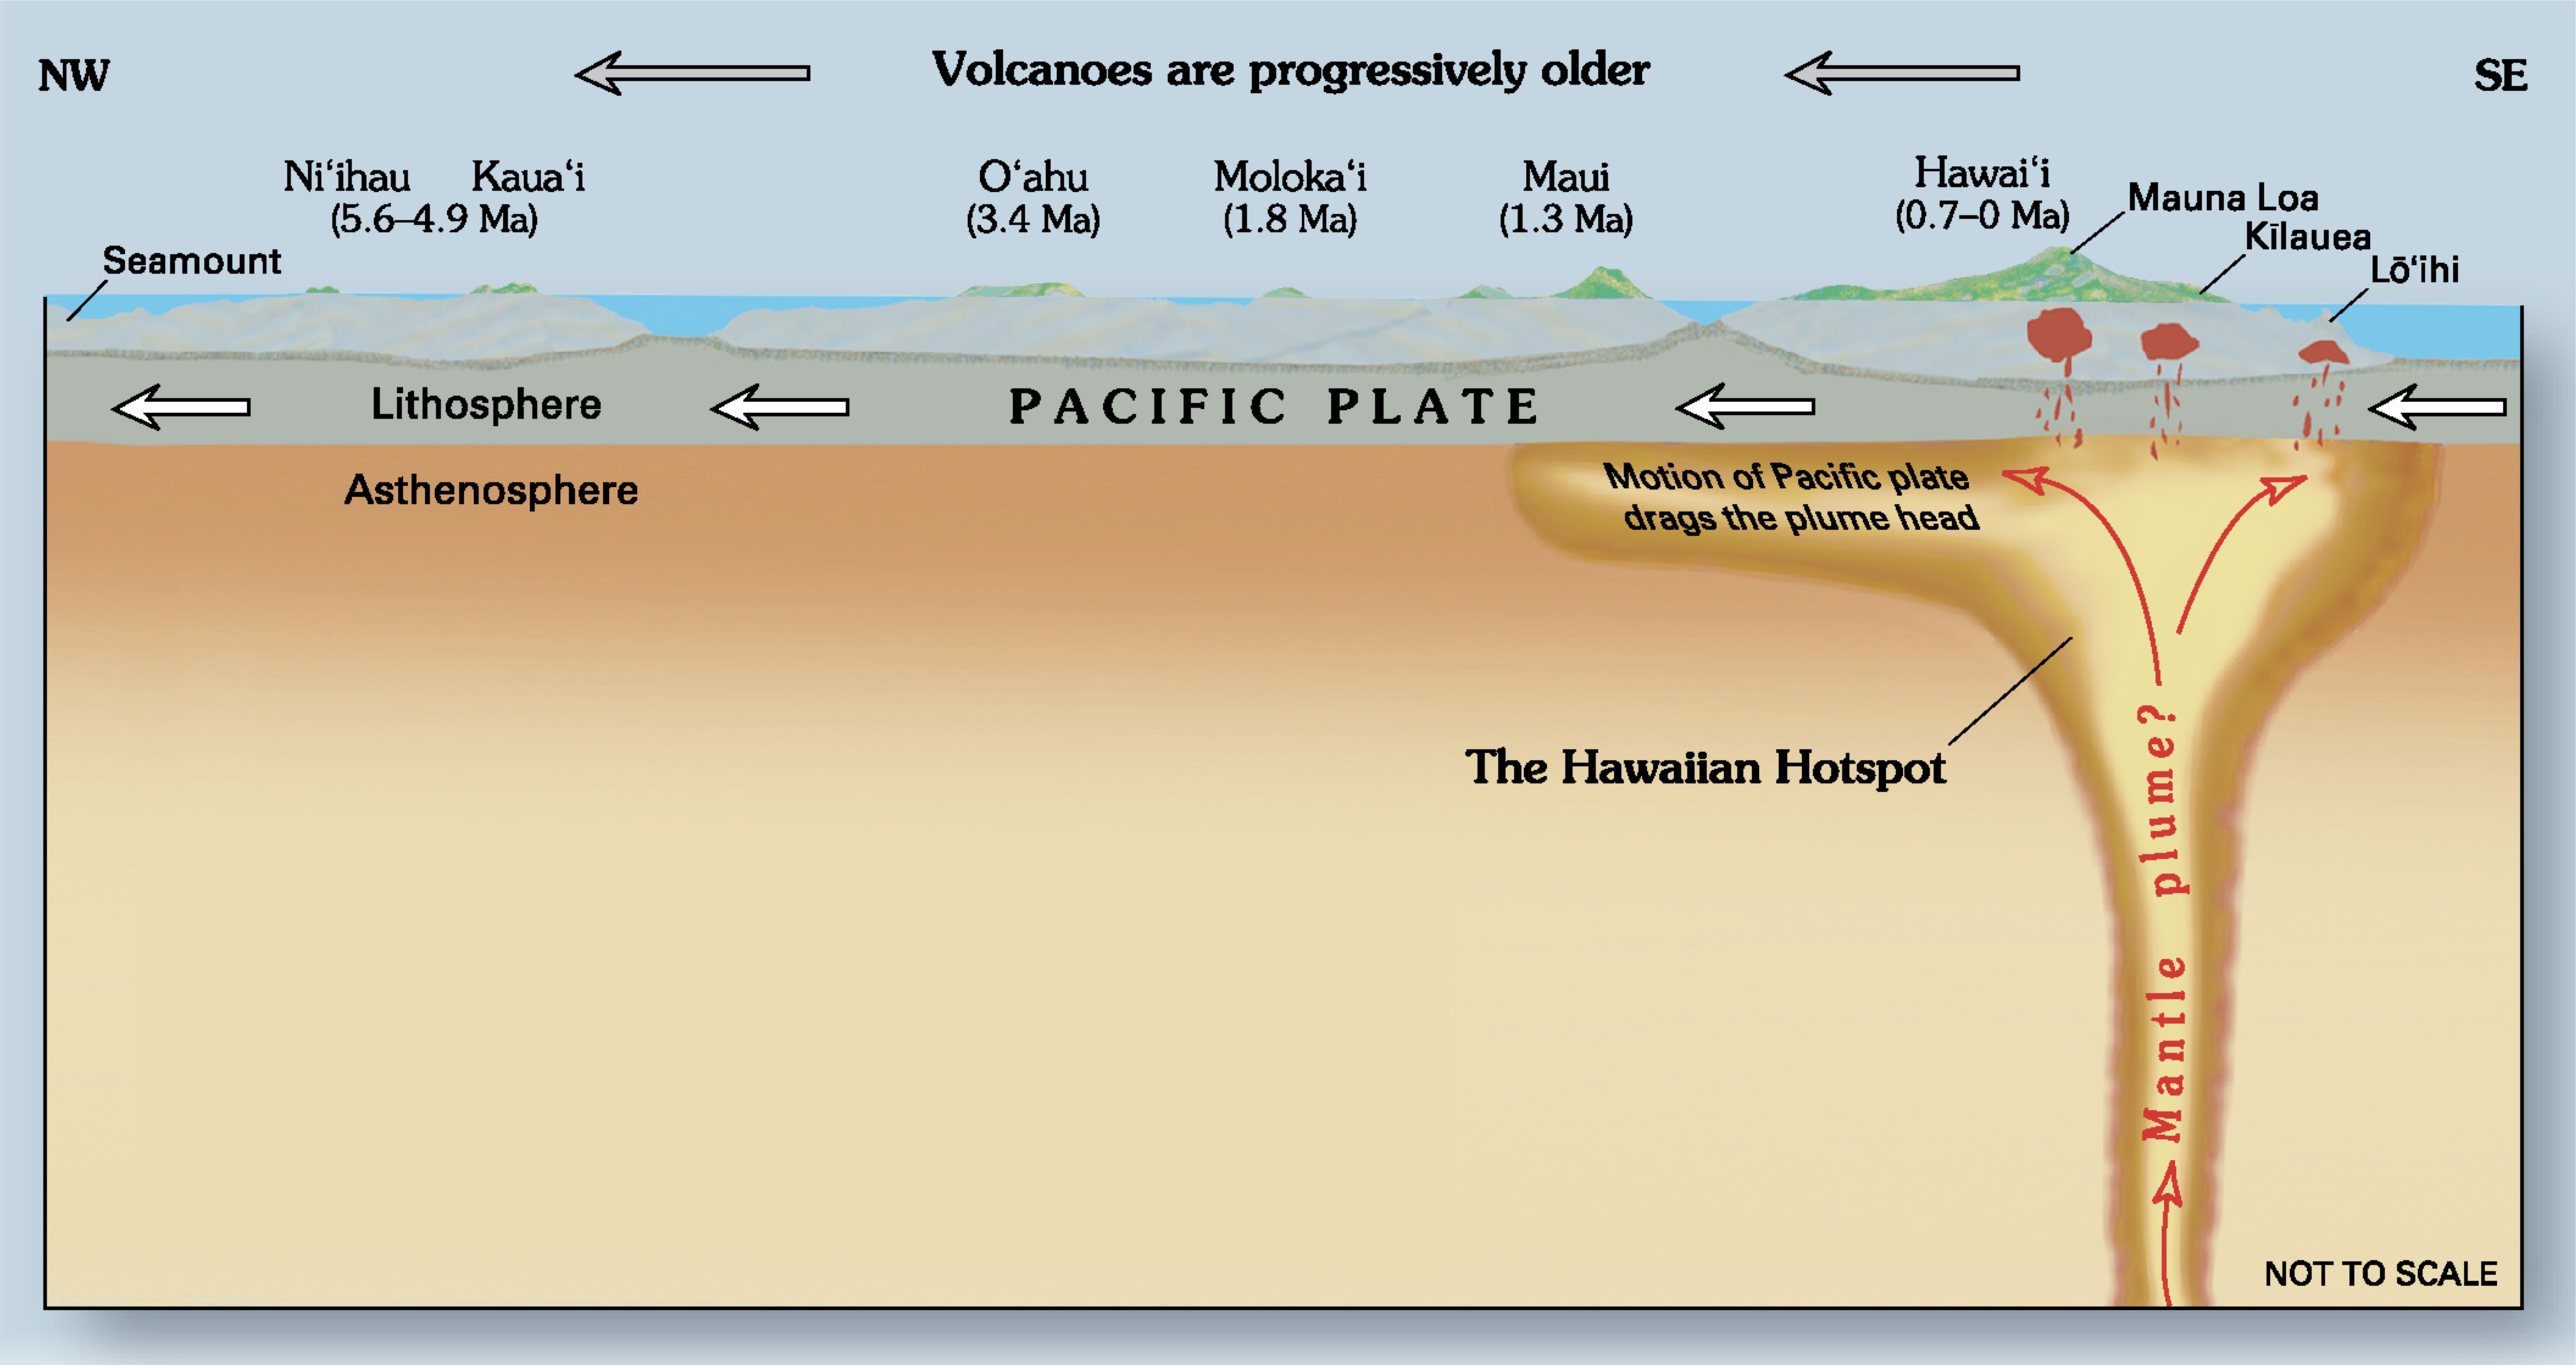
\includegraphics{obrazky/tectonic/Hawaii_hotspot}
	\caption{Diagram zobrazující Havajskou horkou skvrnu (Autor Joel E. Robinson, USGS).}
	\label{fig:hawaiihotspot}
\end{figure*}

\section{Globální geomorfologie}
\subsection{Globální hypsometrie}
Histogram nadmořských výšek (a hloubek) má bimodální charakter. První vrchol odpovídá oceánským pánvím, druhý kontinentálním platformám.

\subsection{Megaformy}
\subsubsection{Formy reliéfu okrajů litosférických desek}
\emph{Konvergentní okraj} je spojen s orogenetickými pochody. Tedy pochody, při nichž dochází ke vzniku pohoří. Jak již bylo řečeno, na konvergentním okraji se litosférické desky pohybují proti sobě. Můžeme rozlišit dva typy konvergentních okrajů a to \textbf{okraje v rovnovážném stavu} a \textbf{kolizní okraje}. Okraje v rovnovážném stavu jsou takové, kde se oceánská litosférická deska podsouvá jinou oceánskou nebo pevninskou desku. Na rozhraní dvou oceánských desek vzniká \textbf{vulkanický ostrovní oblouk}. Příkladem jsou souostroví v Tichém oceánu. Pokud se oceánská deska podsouvá pod pevninskou, vznikají \textbf{orogénní pásma na okrajích kontinentů} a jedná se o tzv. aktivní okraj kontinentu. Kolizní rozhraní litosférických mají řadu forem v závislosti na podobě jejich okrajů. Prvním příkladem je kolize dvou kontinentů. K tomu dochází v situaci, kdy subdukující deska nese na svém okraji kontinentální kůru. Dochází tak k postupnému přiblížování kontinentů a jejich následné kolizi. To vede ke vzniku vnitrokontinentálních kolizních orogénů. Typickým příkladem takového orogénu jsou Himaláje. Původní subdukční zóna je přeměněna na suturní zónu, kde jsou dva kontinenty do sebe stmeleny. Druhý typ kolize nastává, když oceánská deska nese ostrovní oblouky a subdukuje pod pevninskou desku. Dochází k nasunutí těchto ostrovů na okrajové kontinentální pohoří, které je tak modifikováno. Třetím type nastává, když původně subudkující oceánská litosférická deska má i svou pevninskou část. Následně dochází ke střetu kontinentu s ostrovním obloukem, vzniká kontinentální okrajový orogén. Následně je subdukce obnovena, ale s opačnou polaritou. Při kolizi ostrovních oblouků a za předpokladu, že nebude subdukován může dojít k uzavření jedné subdukční zóny, případně k obrácení.

\emph{Divergentní okraj} neboli extenzní zóna se vyznačuje vznikem nové zemské kůry. Většina divergentních okrajů se nachází uprostřed oceánů, kde tvoří středooceánské hřbety. V případě pevniny vznikají v místech divergentního okraje rozsáhlé riftové zóny jako je např. 
\textbf{Kontinentální rifty} jsou protáhlé sníženiny na povrchu kontinentů. Jsou tvořeny pokleslou krou a bočními, relativně vyzdviženými bloky, které jsou směrem ke dnu riftu omezeny poklesovými zlomy. Rozlišujeme \textbf{aktivní rifting}, který je vyvolán vyklenutím území magmatickým tělesem a \textbf{pasivní rifting}, který je indukován až po průniku magmatu v důsledku ztenčení litosféry. V případě aktivního riftingu existuje nejprve vyklenutí a až posléze se vyvíjí riftové údolí, v případě pasivního riftinngu je tomu naopak. Rift je první fází vývoje tzv. pasivního okraje kontinentu.

\emph{Transformní okraj} může vypadat jako jednoduchá zlomová linie nebo složitá zlomová zóna. U transformních okrajů nedochází zpravidla jen k pohybu podél zlomů, ale dochází k lokalizované kompresi či extenzi. Vznikají tak sníženiny \textit{pullapart basins} respektive transpresní hřbety.

\subsubsection{Formy reliéfu vnitřku kontinentů}
Centrální části kontinentů se skládají z kratonů. \emph{Kraton} je stará a stabilní část zemské kůry. Skládají se ze \emph{štítu} (\textit{shield}), který je tvořen krystalickými horninami (metamorfity, magmatické) komplexně deformovanými. Sedimentární pokryv štítů takřka chybí. Druhou částí kratonu je \emph{platforma} (\textit{platform}). Jedná oblast tvořenou mladšími, tektonicky nedeformovanými sedimentárními horninami 

\textbf{Kontinentální pánve} jsou sníženiny (deprese) rozsáhlých rozměrů. Mají plochý reliéf a typická je pro ně velká mocnost sedimentů. Je několik mechanismů, kterým mohou vznikat. Jedná se o tektonické poklesy, termickou izostázi v důsledku ochlazování zemské kůry Dále mohou vznikat zaplňováním iniciální deprese sedimenty. Ty zatěžují zemskou kůru a dochází k dalším poklesům tzn. je tam pozitivní zpětná vazba. Zátež centra - pokles, snos sedimentů z okolních vyvýšenin a následný kompenzační výzdvih na okrajích.

% TODO: \usepackage{graphicx} required
\begin{figure*}
	\centering
	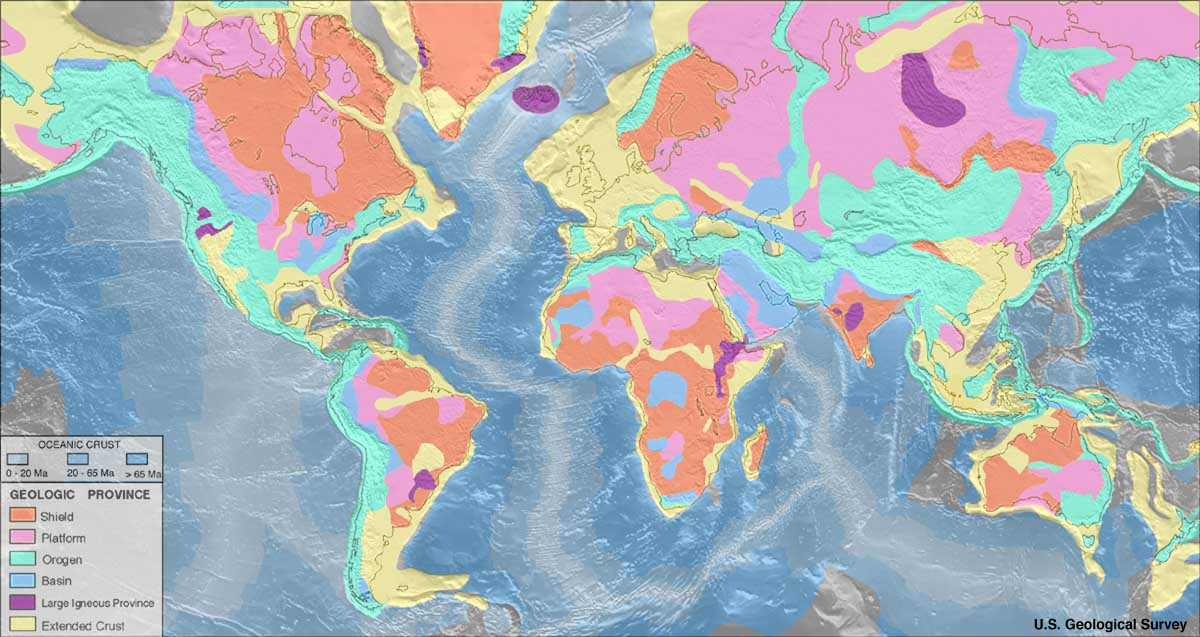
\includegraphics[width=1\linewidth]{obrazky/tectonic/World_geologic_provinces}
	\caption{Mapa geologických provincií (USGS, volné dílo, via Wikimedia Commons)}
	\label{fig:worldgeologicprovinces}
\end{figure*}

		
	\chapter{Tektonické formy a procesy}
	Tektonická geomorfologie studuje tektonické tvary reliéfu a procesy, které tyto tvary utvářejí.

\section{Síla a napětí}
Na horniny v zemské kůře působí gravitační a tektonické síly, které v horninách vyvolávají \emph{napětí}. Napětí je přímo úměrné síle a nepřímo úměrné ploše, na kterou působí. Zapsat to tedy můžeme jako: 

\begin{equation}\label{eq:napeti}
	\text{napětí} = \text{síla}/\text{plocha}
\end{equation}

Celkové napětí lze rozdělit do tří na sebe kolmých komponent -- \emph{hlavních (principiálních) napětí}: $\sigma_{1}$ (největší), $\sigma_{2}$ (střední) a $\sigma_{3}$ (nejmenší napětí).
%\todo[inline]{vložit obrázek kostka napětí}.

\section{Tektonický režim}

Tektonické pohyby mohou reliéf ovlivňovat jak ve vertikálním i horizontálním směru. Při vertikálních posunech dochází ke změně nadmořské výšky, což vede ke změně energie reliéfu a tedy k urychlení odnosu a akumulace. Horizontální pohyby mění topografické uspořádání forem reliéfu, dochází ke změnám v půdorysu. 

Na základě uspořádání principiálních napětí můžeme rozlišit tři základní tektonické režimy:
\begin{itemize}
	\item Extenze
	\item Komprese
	\item Směrový posun
\end{itemize}
%TODO přidat napěťovou kostku
Při \emph{extenzi} dochází k roztahování zemské kůry a ztenčování, což se projevuje poklesovými zlomy. Při \emph{kompresním} režimu dochází ke zkracování zemské kůry. To vede ke vzniku vrás, přesmyků či příkrovů. U směrových posunů dochází k pouhému posouvání ker zemské kůry podél sebe v opačném směru. Pokud je horizontální posun kombinován i s vertikální složkou hovoříme o \emph{transpresním}, respektive \emph{transtenzním} režimu.

Tektonické pohyby rozlišujeme podle stáří. \emph{Paleotektonické} pohyby se projevují pouze ve struktuře. Reliéf mohou ovlivňovat jen pasivně. {Neotektonické} pohyby se projevují v současném reliéfu. Do neotektonických pohybů patří i současné pohyby zemské kůry.

Tektonické pohyby se rozlišují i podle toho, zda je při nich narušena spojitost hornin. \emph{Plikativní (duktilní, vrásové)} pohyby jsou spojité. Jedná se o plastickou deformaci hornin a není tak narušena jejich spojitost. \emph{Disjunktivní (zlomové)} pohyby jsou nespojité, dochází k rozpojení hornin, průběžnost vrstev je narušena.

\section{Zlomy}
Jako \emph{zlom} (\enquote{fault}) se běžně označuje plocha (diskontinuita), v horninovém tělese, podél které došlo k pohybu horninových bloků -- jejich dislokaci. Ve skutečnosti je zlom trojrozměrné těleso jehož třetí rozměr (tloušťka) je zanedbatelný. Zlom vymezují \emph{zlomové plochy}, na kterých bývají stopy pohybu -- \emph{striace}. Zlom odděluje dva bloky (kry) zemské kůry. Pokud je zlom ukloněn, kra nad zlomem se označuje jako \emph{nadložní} (\enquote{hanging-wall}) a kra pod zlomem jako \emph{podložní} (\enquote{foot-wall}).

Podle smyslu pohybu bloků dělíme zlomy na (Obr. \ref{fig:zlomy}):
\begin{itemize}
	\item Poklesové (normální)
	\item Přesmyky (reverzní zlomy)
	\item Horizontální posun
\end{itemize}

\begin{figure}[h]
	\centering
	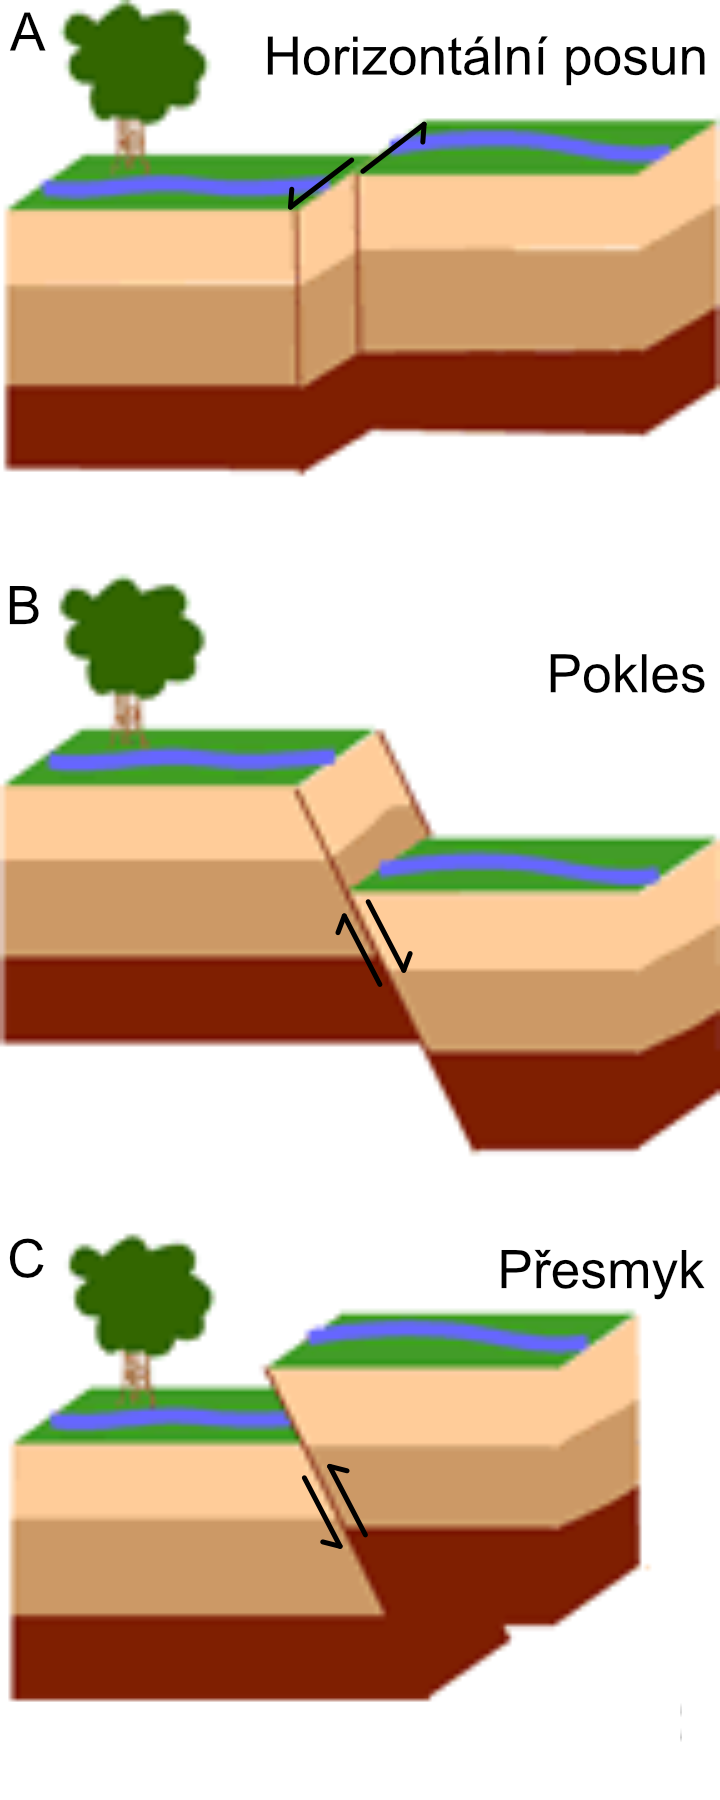
\includegraphics[width=0.8\linewidth]{obrazky/tectonic/zlomy}
	\caption{Typy zlomů. A horizontální posun (levostranný), B pokles, C přesmyk (upraveno podle USGS, volné dílo).}	
	\label{fig:zlomy}
\end{figure}

\subsection{Typy zlomů}
\subsubsection{Horizontální posun}
\emph{Horizontální (směrný) posun} (Obr. \ref{fig:zlomy}A) je zlom charakteristický horizontálním posunem bloků ve směru paralelním k průběhu zlomu. Horizontální posuny velkých rozměrů se nazývají transformní zlomy (viz desková tektonika).

Na základě směru posunu dělíme horizontální posun na pravostranný (dextrální) a levostranný (sinistrální). Orientaci zlomu poznáme jednoduše. Postavíme se čelem ke zlomu a směr určíme podle pohybu protilehlé kry vůči našemu stanovišti Při pravostranném zlomu se protilehlá kra hnula doprava, u levostranného zlomu je tomu naopak. 

Horizontální posuny jsou seismicky nejaktivnější typ zlomů. Typickým příkladem transformního zlomu je zlom San Andreas (Obr. \ref{fig:san_andreas}).

\begin{figure}
	\centering
	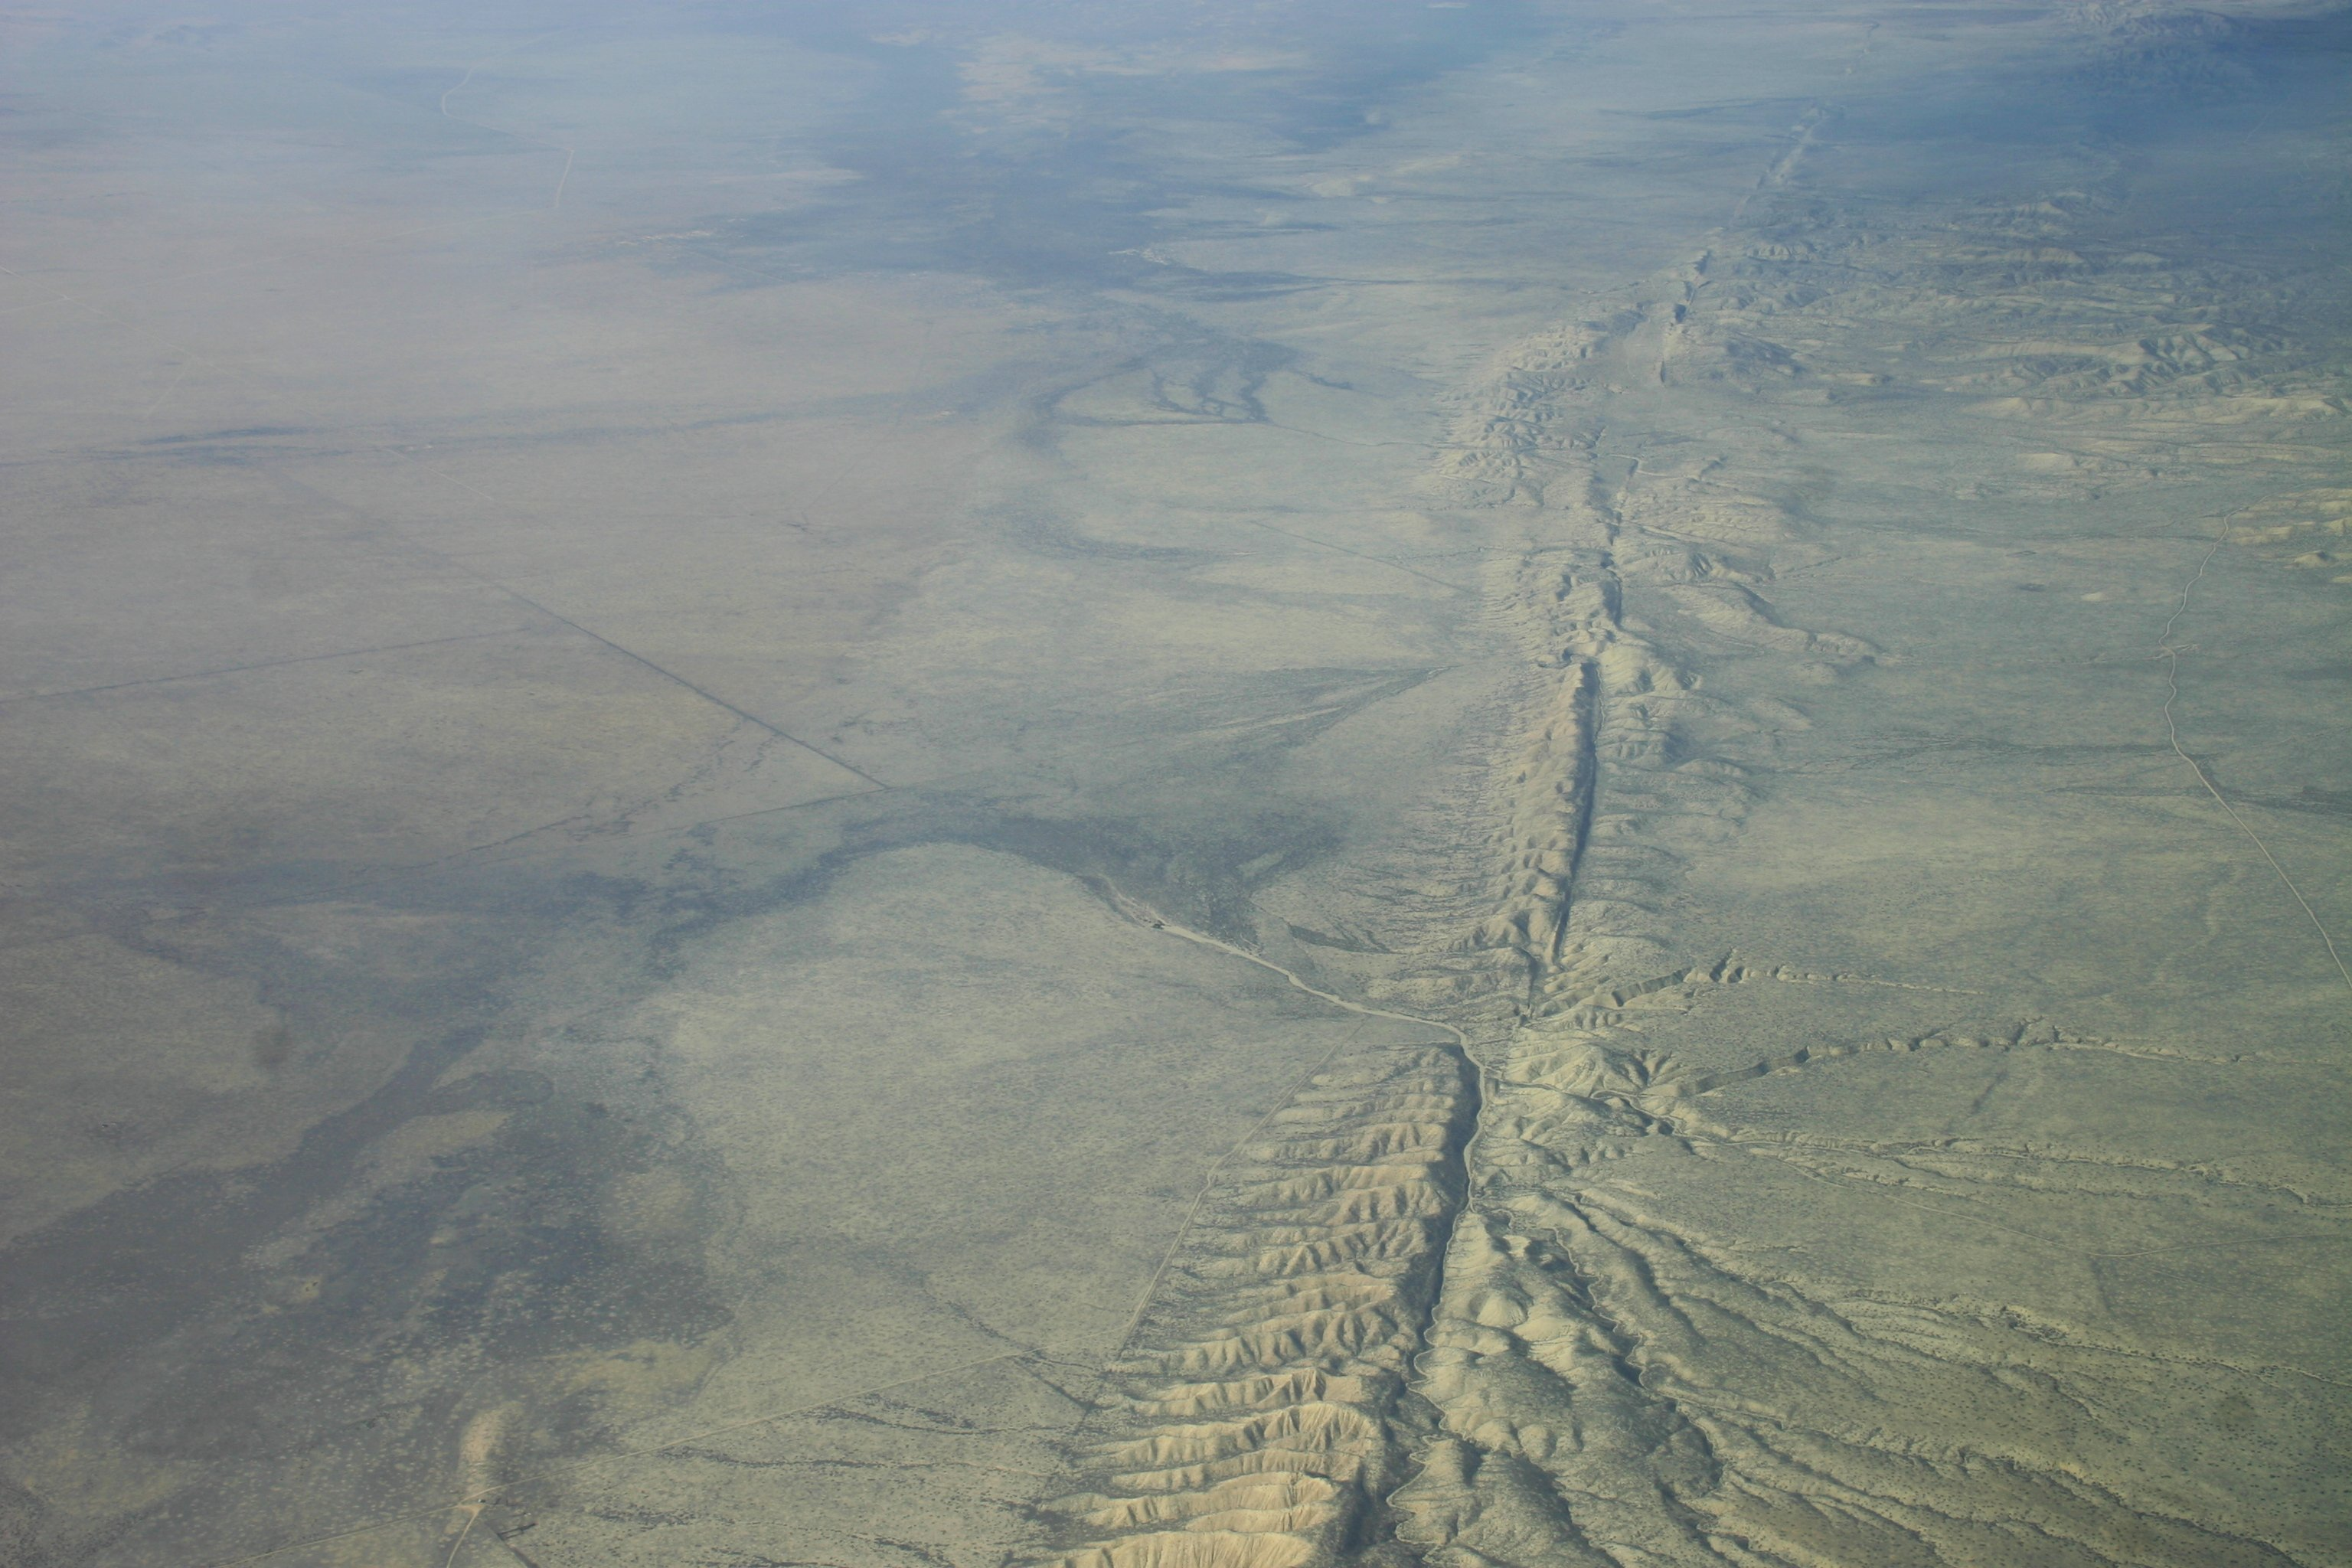
\includegraphics[width=1\linewidth]{obrazky/tectonic/san_andreas}
	\caption{Pohled na zlom San Andreas, Carrizo Plain (autor Ian Kluft, CC-SA 4.0)}
	\label{fig:san_andreas}
\end{figure}

Horizontální posuny se v reliéfu projevují víceméně přímočarými liniemi, jelikož jsou převážně vertikální. Směrným posunem dochází k ohybům vodních toků. 

Zřídkakdy je průběh zlomu zcela rovný. V místech ohybů tak dochází k lokální extenzi \emph{(transtenze)} nebo kompresi \emph{(transprese)}. Extenzí vznikají poklesy, tzv. \emph{pull apart pánve}. Při kompresi dochází k výzdvihu zemské kůry a vzniku \emph{kompresních hřbetů}.

\subsubsection{Pokles}
\emph{Poklesové zlomy} (\enquote{normal fault}) (Obr. \ref{fig:zlomy}B, \ref{fig:pokles}) jsou důsledkem extenze zemské kůry. Jsou charakteritické velkým sklonem (\SIrange{50}{60}{\degree}) vzhledem k povrchu. Poklesává nadložní kra. Tedy podložní kra je ve vyšší pozici oproti nadložní kře. 

Velké poklesové zlomy mají \emph{listrický} tvar. To znamená, že jsou konkávně zakřivené. S hloubkou se jejich sklon zmenšuje někdy až do horizontální pozice. V případě zakřivených poklesových zlomů vznikají oproti nim sekundární poklesové zlomy, které mají opačný směr sklonu a smysl pohybu. Označují se jako tzv. \emph{antitetické zlomy}.

\begin{figure}
	\centering
	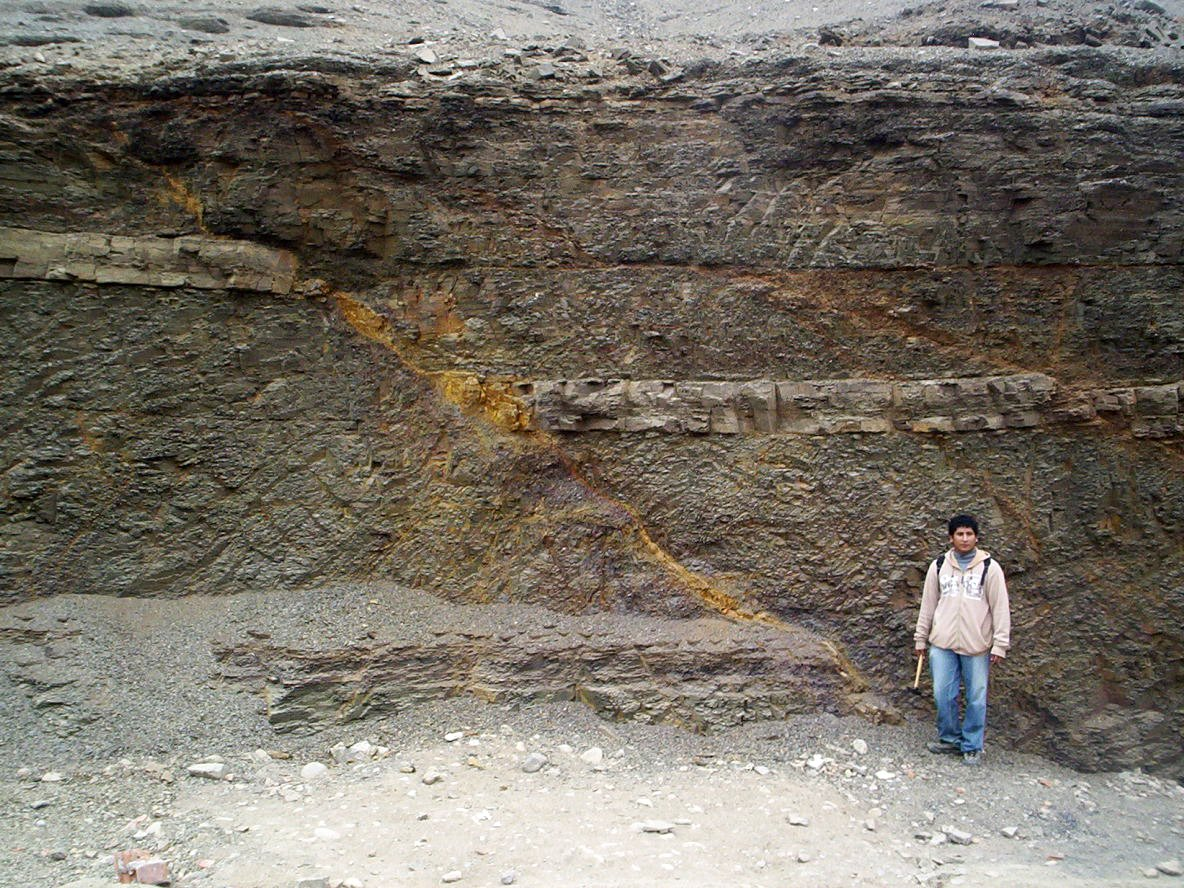
\includegraphics[width=1\linewidth]{obrazky/tectonic/pokles}
	\caption{Příklad normálního (poklesového zlomu) v v souvrství La Herradura. Lokace Morro Solar Lima, Peru (autor: Miguel Vera León)}
	\label{fig:pokles}
\end{figure}

\subsubsection{Přesmyk}
\emph{Přesmyk} (\enquote{reverse fault}) (Obr. \ref{fig:zlomy}C) je důsledkem komprese (zkracování) zemské kůry. Se zkracováním narůstá mocnost kůry. Přesmyky jsou charakteristické menším sklonem, který se pohybuje okolo \SI{30}{\degree}. Nadložní kra se nasouvá na podložní. Nadložní kra se tak nachází ve vyšší pozici než kra podložní. 
Přesmyky dělíme na kerné, které jsou čistou střižnou deformací, a vrásové, které vznikly přetrhnutím jednoho ramena vrásy.

\subsubsection{Násun}
\emph{Násun} (\enquote{thrust}) je specifickým typem přesmyku. Úklon násunu je zpravidla velice mírný až subhorizontální. 

\subsection{Projev zlomů v reliéfu}
\subsubsection{Zlomový svah}
Nejběžnějším projevem vertikálního pohybu na zlomech je \emph{zlomový sráz, stupeň} (\enquote{fault scarp}) (Obr. \ref{fig:faultscarp}). Zlomové stupně často vznikají při zemětřeseních (koseismické pohyby). Dlouhodobou kumulací pohybů při zemětřeseních, případně vytrvalým výzdvihem jedné kry (resp. poklesem druhé), tzv. interseismickými pohyby, se vyvíjí \emph{zlomový svah}. Okraje pohoří vyzdvižených podél zlomů jsou charakteristické tzv. facetami. Jsou to trojúhelníkové nebo lichoběžníkové plochy vzniklé rozčleněním a přemodelováním zlomových svahů erozí (obr. \ref{fig:facety}). Jejich sklon je nižší, než sklon zlomových svahů. Typicky se pohybuje mezi \SIrange{25}{35}{\degree}.

\begin{figure*}[h]
	\centering
	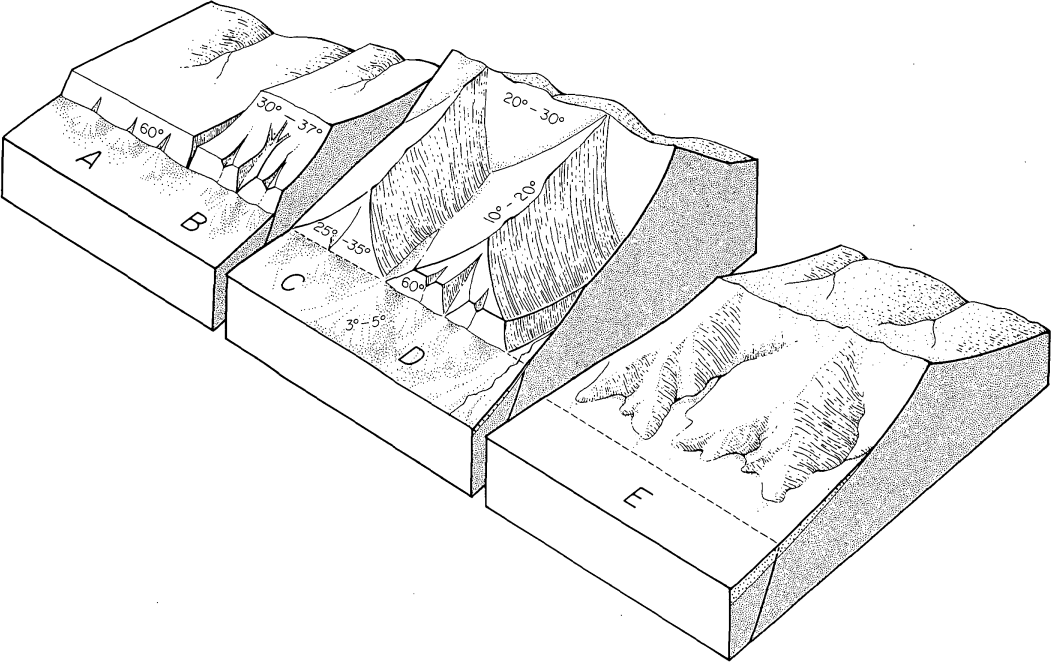
\includegraphics[width=1\linewidth]{obrazky/tectonic/facety}
	\caption{Ukázka vývoje zlomového okraje pohoří a vzniku facet. A: čerstvý zlomový svah; B: postupné zařezávání vodních toků (strže), přemodelování zlomového stupně; C,D: vyvinutá údolí a facety, opakovaný nebo intenzivní výzdvih udržuje zlomový svah (D); E: dlouhé období tektonického klidu, postupná denudace (převzato z \textcite{wallaceGeometryRatesChange1978})}
	\label{fig:facety}
\end{figure*}




\begin{figure*}[h]
	\centering
	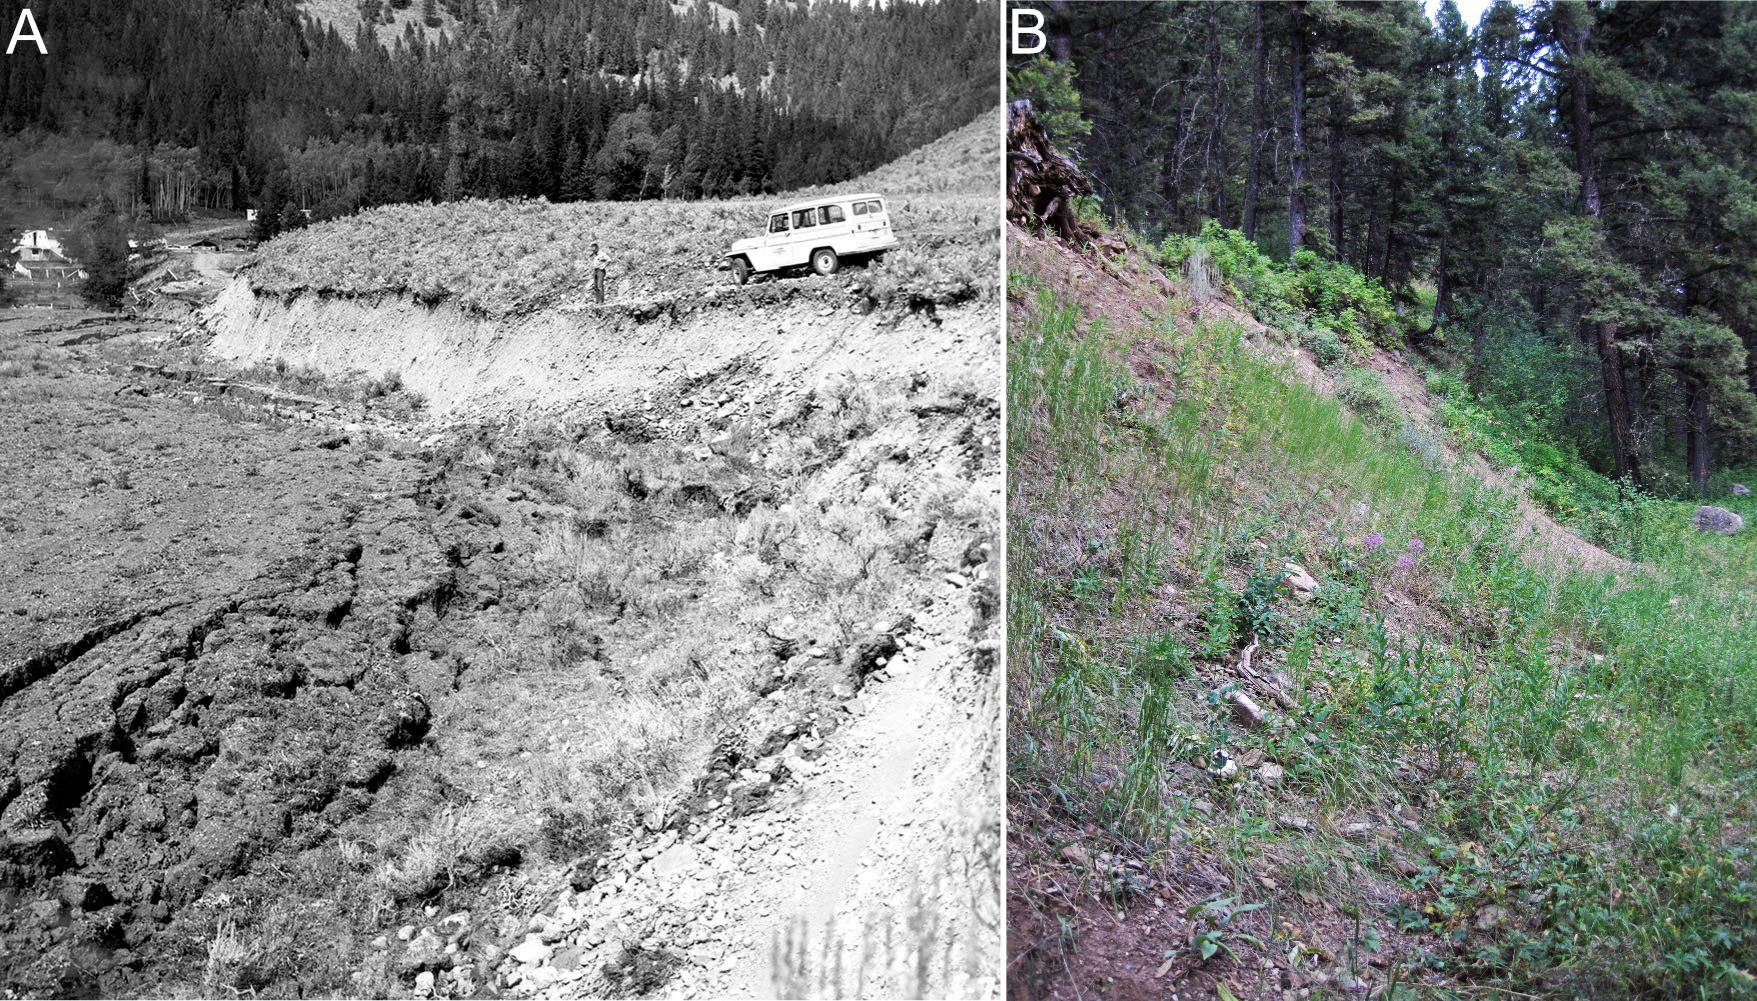
\includegraphics[width=1\linewidth]{obrazky/tectonic/fault_scarp}
	\caption{Zlomový sráz, který vznikl při Yellowstonském zemětřesení v roce 1959. A fotografie pořízená těsně po události (autor J. R. Stacy, USGS, volné dílo/Public Domain). B Stupeň již částečně zhlazený difuzními procesy o 59 let později (autor James St. John, CC BY 2.0).}
	\label{fig:faultscarp}
\end{figure*}

Rychlost degradace zlomového srázu je daná především pevností dané horniny. Větší rychlostí bude degradovat stupeň vzniklý v nezpevněných sedimentech, než v pevných horninách. Dalším faktorem je intenzita exogenních procesů, tedy jak intenzivně na sráz působí voda a podobně. 

Rychlost pohybu na zlomu ovlivňuje podobu zlomových svahů. Zlomové svahy na poklesových zlomech s rychlým pohybem mají výrazné a málo degradované facety, údolí členící zlomový svah jsou úzká a hluboce zařezaná. Při pomalém pohybu na zlomu jsou facety degradované, údolí zařezávající se do podložní kry jsou široká a v předpolí se nachází velké, mírně ukloněné výplavové kužely, do kterých je zaříznutý vodní tok. 

Pohybem na zlomu může dojít k tomu, že na jedné straně zlomové plochy se nacházejí méně odolné horniny, než na straně druhé. Jelikož eroze bude postupovat rychleji v méně odolných horninách, může vzniknout nový svah tzv. \emph{svah na zlomové čáře}. Podle orientace nového svahu vůči zlomu jej dělíme na tzv. resekventní svah, který má stejnou orientaci jako původní zlomový svah, a obsekventní svah s opačnou orientací.

\subsubsection{Hrástě a prolomy}
V soustavě paralelních zlomů vznikají hrástě a prolomy. \emph{Hrásť} (\enquote{horst}) je protáhlá vyvýšenina. Jedná se o kru, která je vůči svému okolí nejvyšší. Hrástě mohou vznikat výzdvihem kry -- je tedy omezena přesmyky, které mají úklon pod vyzdviženou kru. Tento typ hrástí označujeme jako \emph{automorfní hrástě}. Hrástě, které vznikly poklesem okolních ker (tedy její omezení je poklesovými zlomy), se nazývají \emph{xenomorfní hrástě}.

Protáhlé sníženiny omezené poklesovými zlomy se nazývají \emph{prolomy} (\enquote{graben}). Prolomy jsou také označovány jako \emph{riftová údolí}.  Pokud je sníženina omezená jedním velkým listrickým zlomem na jedné straně a případnými kompenzčními antetickými zlomy na druhé, hovoříme o tzv. \emph{polo-prolomech} (\enquote{half-graben}). V prolomech a  poloprolomech se ukládá velké množství sedimentů z okolních elevací. Mocnost sedimentů může být enormní - až v řádu kilometrů.

Taktéž může nastat, že se jedna kra ukloní -- na jedné straně dojde k jejímu poklesu, na opačné pak k výzdvihu. 

\subsubsection{Projevy horizontálních pohybů}

Horizontální pohyby mohou ovlivnňovat reliéf pasivně tím, že bude docházet k selektivní erozi podél tektonicky oslabených hornin. Aktivní ovlivnění reliéfu horizontálními pohyby se projevuje v dislokaci geomorfologických a jiných krajiných prvků. Dochází tak ke zmenám v půdorysu. Nejvíce je to patrné na geomorfologických sítích (vodní toky).

Jedním z důsledků horizontálního posunu může být například posunutí průběhu hřbetů a údolí.

\subsubsection{Příkrovy}
\emph{Příkrovy} (\enquote{nappes}) jsou rozsáhlá tělesa přesunutá podél násunových zlomů na vzdálenost minimálně 5 km. Běžně se jedná ale o přesuny až na vzdálenost desítek kilometrů. Příkrov (přesunuté těleso) se označuje jako \emph{alochton}, stabilní podloží je \emph{autochton}.

\section{Pukliny}
\emph{Pukliny} (\enquote{joints}) jsou diskontinuity podél kterých nedošlo k pohybu nebo byl neznatelný. Pukliny jsou nejrozšířenějším typem diskontinuit. Jejich klasifikace je založená na základě celé řady kritérií (tvar, velikost, frekvence,...). Pukliny mohou být systematické (systém subparalelních puklin) a nesystematické (nepravidelné, zakřivené). 

Pukliny mohou pasivně ovlivňovat vývoj reliéfu, jelikož to jsou místa oslabení horninového masivu. Může jimi například snadno pronikat voda a urychlovat zvětrávání a erozi horniny. Pěkně je tento vliv puklinových systémů na reliéf vidět u pískovcových skalních měst. Soutěsky se vyvíjejí podél jednotlivých puklinových systémů, na kterých koncentruje erozní činnost.

\section{Vrásy}
\emph{Vrásy} (\enquote{folds}) vznikají duktilní deformací hornin. Jedná se o spojité tektonické struktury. K vrásnění dochází při kompresním režimu, kdy se ohybem planárních struktur hornin (např. vrstev) zkracuje zemská kůra. Jednoduché prohnutí vrstev je označováno jako \emph{flexura}. Narozdíl od vrás mohou flexury vznikat i v extenzním režimu. Vrásy jsou často ve spojení se zlomy.

Rozlišujeme \emph{antiklinálu}, což je část, která je vyklenutá vzhůru a \emph{synklinálu}, jejíž vyklenutí je směrem dolů. Část, která spojuje antiklinálu a synklinálu, se nazývá \emph{rameno vrásy} nebo také křídlo vrásy.

\begin{figure}[h]
	\centering
	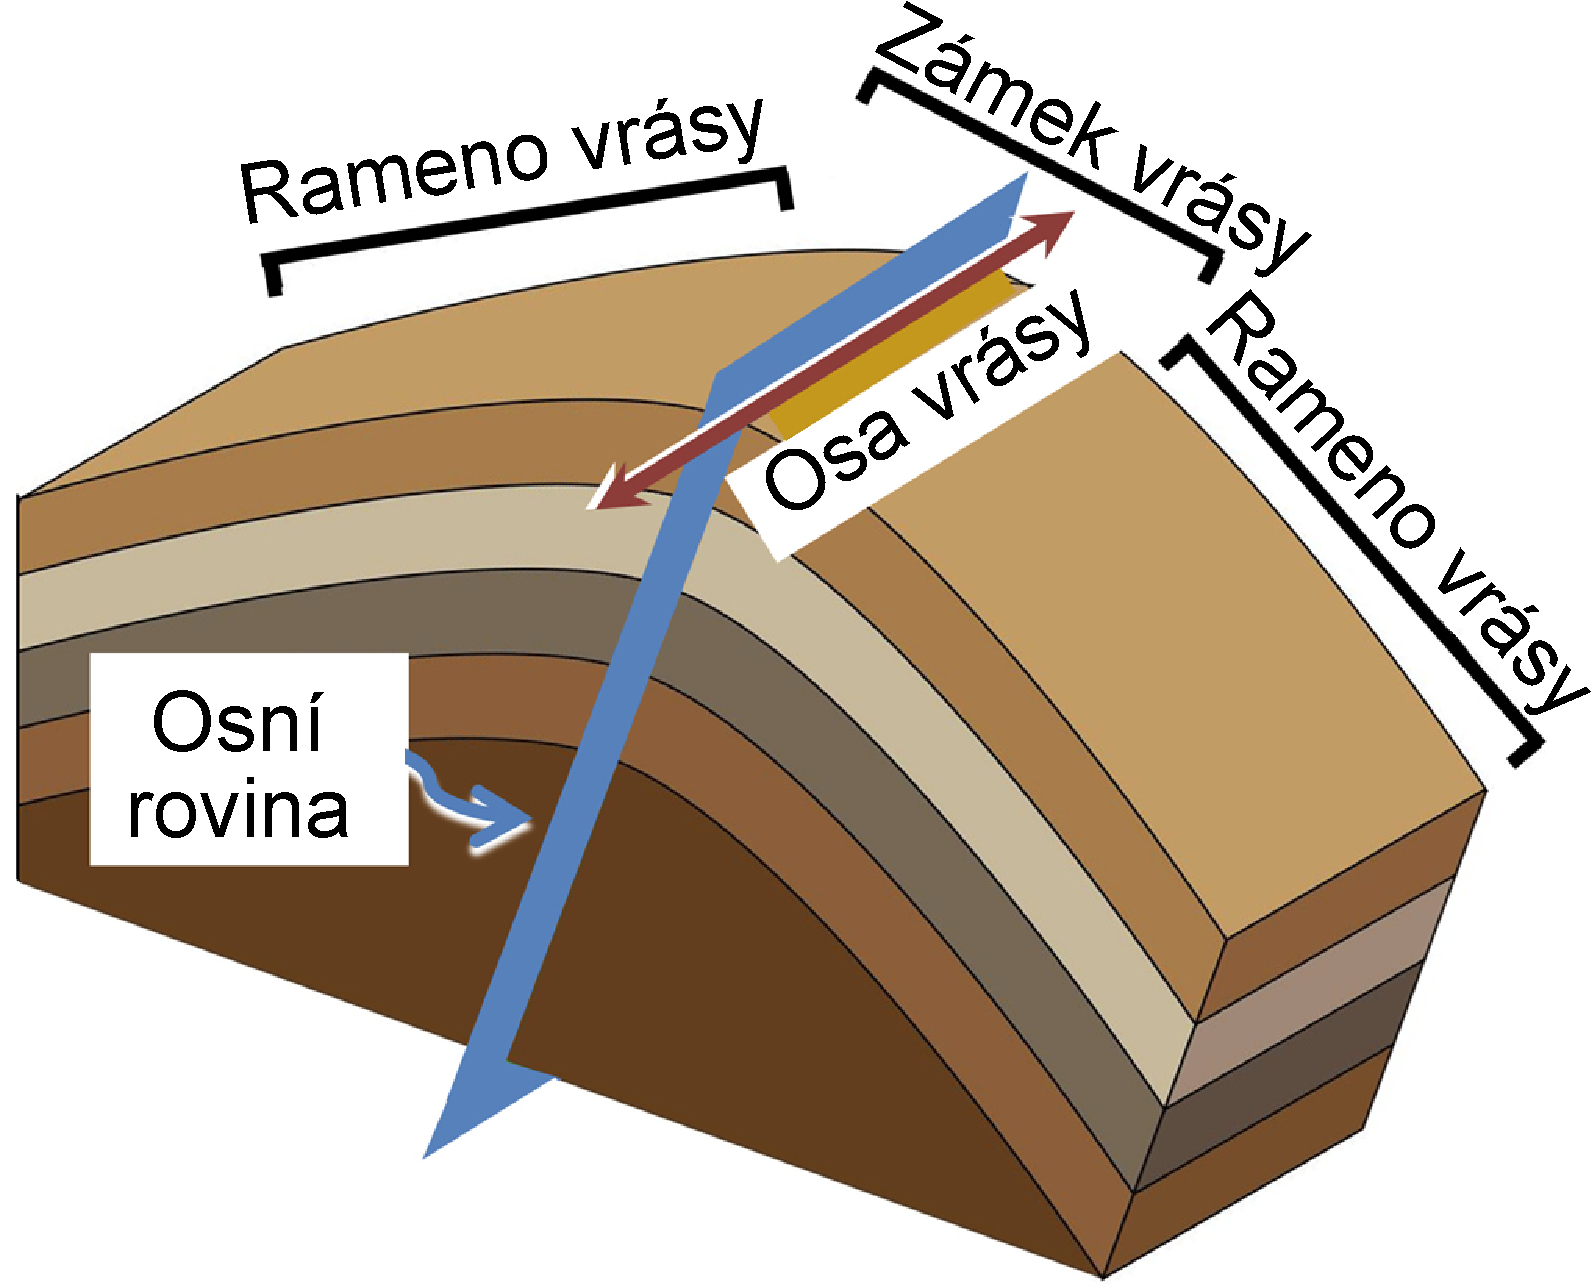
\includegraphics[width=\linewidth]{obrazky/tectonic/fold_parts}
	\caption{Části vrásy (Upraveno podle Brews Ohare, CC BY-SA 3.0)}
	\label{fig:foldparts}
\end{figure}

Vrásy dělíme podle osní roviny na:

\begin{itemize}
	\item vzpřímené
	\item ukloněné
	\item převrácené
	\item ležaté
\end{itemize}

Další dělení vrás je podle sevřenosti jejich ramen:
\begin{itemize}
	\item rozevřené
	\item otevřené
	\item sevřené
	\item zavřené
	\item izoklinální
\end{itemize}

Vrásy také můžeme rozdělit na symetrické a nesymetrické. V případě prohnuté osy vrásy hovoříme o tzv. brachyantiklinálách a brachysynklinálách.

\subsection{Izometrické vrásy}
Specifickou formou vrás jsou tzv. izometrické vrásy. Jedná se o vrásové struktury, které nejsou protažené jedním směrem. 

Synklinální sníženiny oválného až kruhovitého půdorysu se nazývají \emph{pánve}. Výraznost pánevních oblastí je daná velikostí prohnutí vrstev (čím větší, tím je pánve výraznější) a na míře zaplnění pánve sedimenty. Na okrajích pánví lze nalézt asymetrické hřbety -- kuesty (viz dále). 

Vyklenutím hornin vzhůru vznikají \emph{klenby}. Jedná se o velká tělesa oválného až kruhového půdorysu. Klenby mohou vznikat intruzí magmatu mezi vrstevní plochy, což způsobuje vyklenutí nadložních vrstev. V takovém případě se jedná o \emph{klenby s krystalickým jádrem}. \emph{Sedimentární klenba} nemá krystalické jádro, vzniká prostým prohntím sedimentárních hornin v důsledku bočních tlaků. K vyklenutí může dojít také kvůli intruzím solných diapirů působením hydrostatických nebo tektonických tlaků. Vznikají tak \emph{solné klenby}. 

\subsection{Projev vrás v reliéfu}
Vztah mezi zvrásněným podložím a georeliéfem může nabývat celé řady podob. Vrásy vytvářejí \emph{vrásová pohoří}. Vazba mezi reliéfem a strukturou může být \emph{přímá} -- v místě antiklinály se nachází hřbet a v místě synklinály údolí. 

Jednoduchá vrásová pohoří jsou tvořená vrásami, které mají jen minimálně zvlněné osy. Tvoří paralelně probíhající soustavu hřbetů a údolí. Takový typ pohoří je označován jako jurský typ reliéfu (podle pohoří Jura ve Švýcarsku). Dalším příkladem je pohoří Zagros v Íránu (Obr. \ref{fig:zagros}). 

Při značném zvlnění os vrás, vznikají složitá vrásová pohoří tvořená soustavou brachyantiklinál a brachysynklinál. Tento typ se označuje jako Apalačský podle pohoří v USA (Obr. \ref{fig:apalachian}).

\begin{figure}[h]
	\centering
	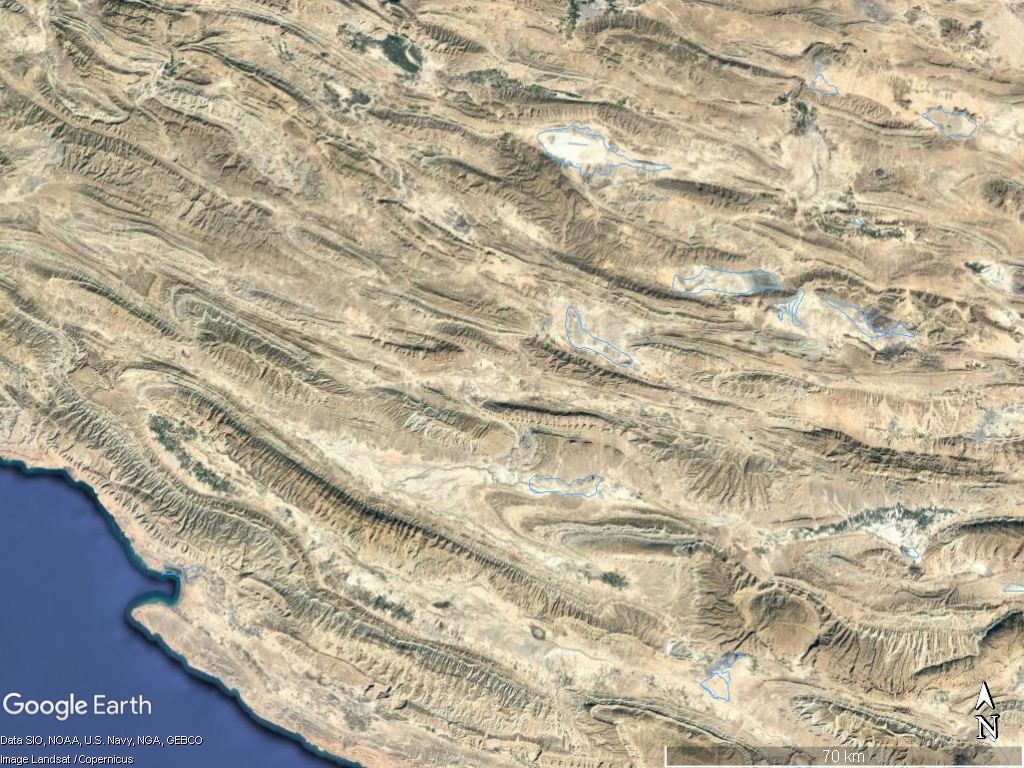
\includegraphics[width=1\linewidth]{obrazky/tectonic/zagros}
	\caption{Pohoří Zagros (zdroj Google Earth)}
	\label{fig:zagros}
\end{figure}

\begin{figure}[h]
	\centering
	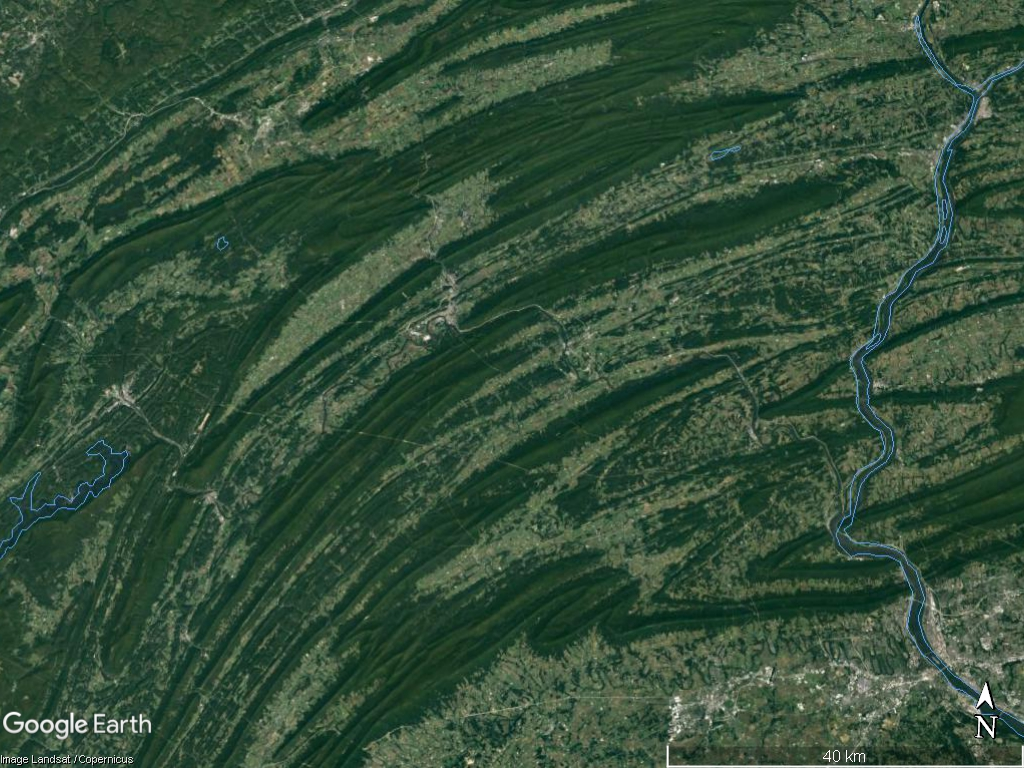
\includegraphics[width=1\linewidth]{obrazky/tectonic/apalachian}
	\caption{Apalačské pohoří v USA (zdroj Google Earth)}
	\label{fig:apalachian}
\end{figure}

Velice často je s vrásami spojená tzv. \emph{inverze reliéfu}. Horniny v ose antiklinály jsou značně tektonicky porušené (rozpukané), jsou tedy i náchylnější k erozi. Dlouhodobým vývojem reliéfu tak dochází k oderodování antiklinály a vzniku \emph{antiklinálního údolí}, kdežto v místech synklinál je z důvodu pomalejší eroze elevace.

\section{Strukturní reliéf}

\begin{figure*}[h]
	\centering
	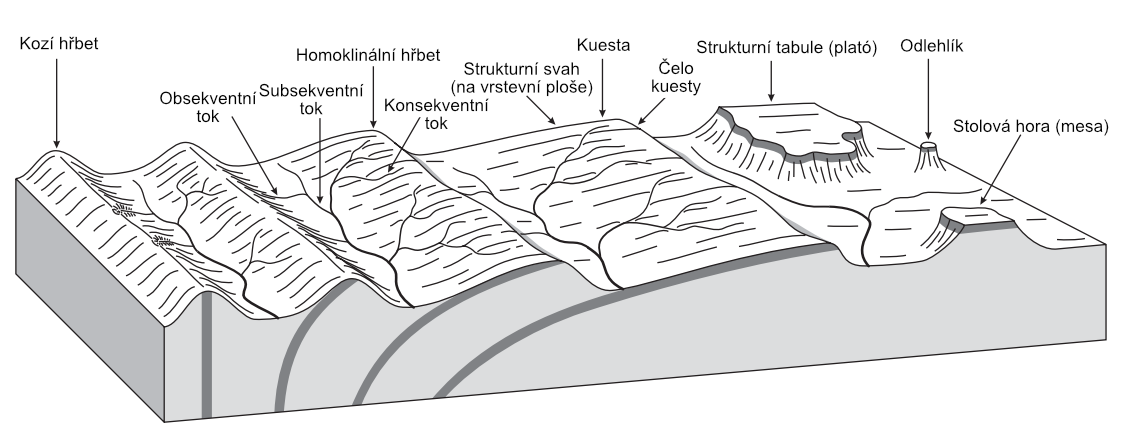
\includegraphics[width=1\linewidth]{obrazky/tectonic/strukturni_tvary}
	\caption{Strukturní reliéf -- tvary na horizontálních a ukloněných vrstvách. Horizontální vrstvy -- strukturní tabule, stolová hora a odlehlík. Ukloněné vrstvy -- kuesta, homoklinální hřbet a kozí hřbet. Označené jsou i základní typy vodních toků. Konsekventní -- ve směru sklonu vrstev, subsekventní -- po směru vrstev a obsekventní -- proti směru sklonu vrstev. Tmavě šedé pásy vyznačují polohy odolných hornin (upraveno podle \textcite{huggettFundamentalsGeomorphology2007}).}
	\label{fig:strukturnitvary}
\end{figure*}

\subsection{Horizontálně uložené vrstvy}
Sedimentární horniny, které nebyly postižené vrásněním mají zpravidla horizontálně až subhorizontálně uložené vrstvy. 
Fluviální erozí a svahovými procesy se v takových oblastech vyvíjí \emph{strukturní tabule} (\textit{plateaux}), což jsou rozsáhlé ploché elevace, které jsou od svého okolí oddělené strmými svahy. Postupným rozrušováním tabule vznikají plošně menší \emph{stolové hory} (\textit{mesa}), \emph{svědecké vrchy} až \emph{odlehlíky} (\textit{butte}) a úzké, vysoké \emph{skalní jehly} (\textit{pinnacles)}. Důležitou podmínkou je přítomnost odolnějších hornin v nadloží (\textit{caprock}), které brání celkové erozi (Obr. \ref{fig:strukturnitvary}).

V oblastech, kde je časté střídání tvrdých (odolných) a měkkých (málo odolných) vrstev, se vyvíjejí \emph{strukturní stupňoviny}. Kdy odolné vrstvy tvoří stupně -- \emph{strukturní terasy}.

\subsection{Ukloněné vrstvy}
Na ukloněných horninách (do \SI{7}{\degree}), které mají různou odolnost, se vyvíjejí asymetrické hřbety -- \emph{kuesty} (Obr. \ref{fig:strukturnitvary}). Čelo kuesty je strmé a vzniklo erozí ukloněných vrstev. Týlní svah je mírný a odpovídá sklonu vrstev (\enquote{dipslope}). Kuesty se často nacházejí ve skupinách a jejich počet odpovídá počtu odolných vrstev. 

Při větším sklonu vrstev (\SIrange{7}{40}{\degree}) vznikají asymetrické hřbety označované jako \emph{homoklinální}. Při sklonu nad \SI{40}{\degree} pak \emph{kozí hřbety}, které mohou být v příčnem profilu již symetrické (Obr. \ref{fig:strukturnitvary}).

%TODO přepsat otazky
\newpage
\onecolumn
\begin{boxotazky}{Kontrolní a klíčové otázky, na které bychom měli znát odpověď}
	\begin{itemize}
		\item Jak odlišíme nadložní a podložní kru?
		\item K čemu dochází z hlediska mocnosti zemské kůry při poklesu a co při násunu?
		\item Jakým způsobem mohou zlomy s horizontální složkou pohybu ovlivnit říční síť?
		\item Vysvětlete inverzi reliéfu. Proč k ní dochází?
		\item Jakým způsobem ovlivňuje uložení sedimentárních hornin georeliéf?
		
	\end{itemize}
\end{boxotazky}

\begin{boxslovnik}{Další klíčové pojmy k zapamatování}
	zlom & puklina \\
	vrása & přesmyk \\
	pokles & násun \\
	mesa & kuesta \\
	kozí hřbet & inverze reliéfu \\
\end{boxslovnik}
\twocolumn

	\chapter{Magmatismus, vulkanické procesy a tvary reliéfu}
	Pohyby magmatu ze zemského pláště do zemské kůry mají za následek celou řadu forem reliéfu. V případě, že se magma dostává na povrch, jedná se o \textbf{extruzivní} magmatismus.  \textbf{Intruzivní} magmatismus dává za vznik formám reliéfu, které jsou patrné až po jejich obnažení.  

\section{Formy reliéfu spojené s intruzemi magmatu}
\subsection{Velká intruzivní tělesa}
Mezi rozsáhlá intruzivní tělesa patří \textbf{batolity}, neboli také \textbf{plutony}. Tvoří je granitoidní horniny. Batolity jsou často v podloží nejvyšších částí kontinentálních orogénů. Intruze magmatu a vznik batolitu může způsobit vyklenutí nadložních sedimentárních hornin. Po exhumaci batolitu erozí nadložních hornin dochází k jeho zvětrávání podél puklin, které jsou organizované zpravidla do třech na sebe kolmých systémů. Obnažení intruzivních těles vede k uvolnňování napětí v hornině a vzniku sekundárních (exfoliačních) puklinových systémů. \textbf{Lopolit} je dalším typem rozsáhlého intruzivního tělesa. Má tvar pánve a je tvořeno bazickými horninami typu gabro. Telěso menšího rozsahu než batolit je \textbf{peň}.

\subsection{Intruzivní tělesa menšího rozměru}
Menší intruzivní tělesa doprovázejí větší intruzivní tělesa či extrusivní tělesa. Můžeme je rozdělit na konkordantní pokud probíhají podél původních vrstevních ploch a na diskordantní v případě jejich protnutí. Mezi diskordantní tělesa patří \textbf{pravé žíly} (Obr. \ref{fig:zila}). Jedná se o \SIrange{1}{10}{\metre} široká tělesa. Vyskytují se nejčastěji ve větších skupinách.

% TODO: \usepackage{graphicx} required
\begin{figure}[h]
	\centering
	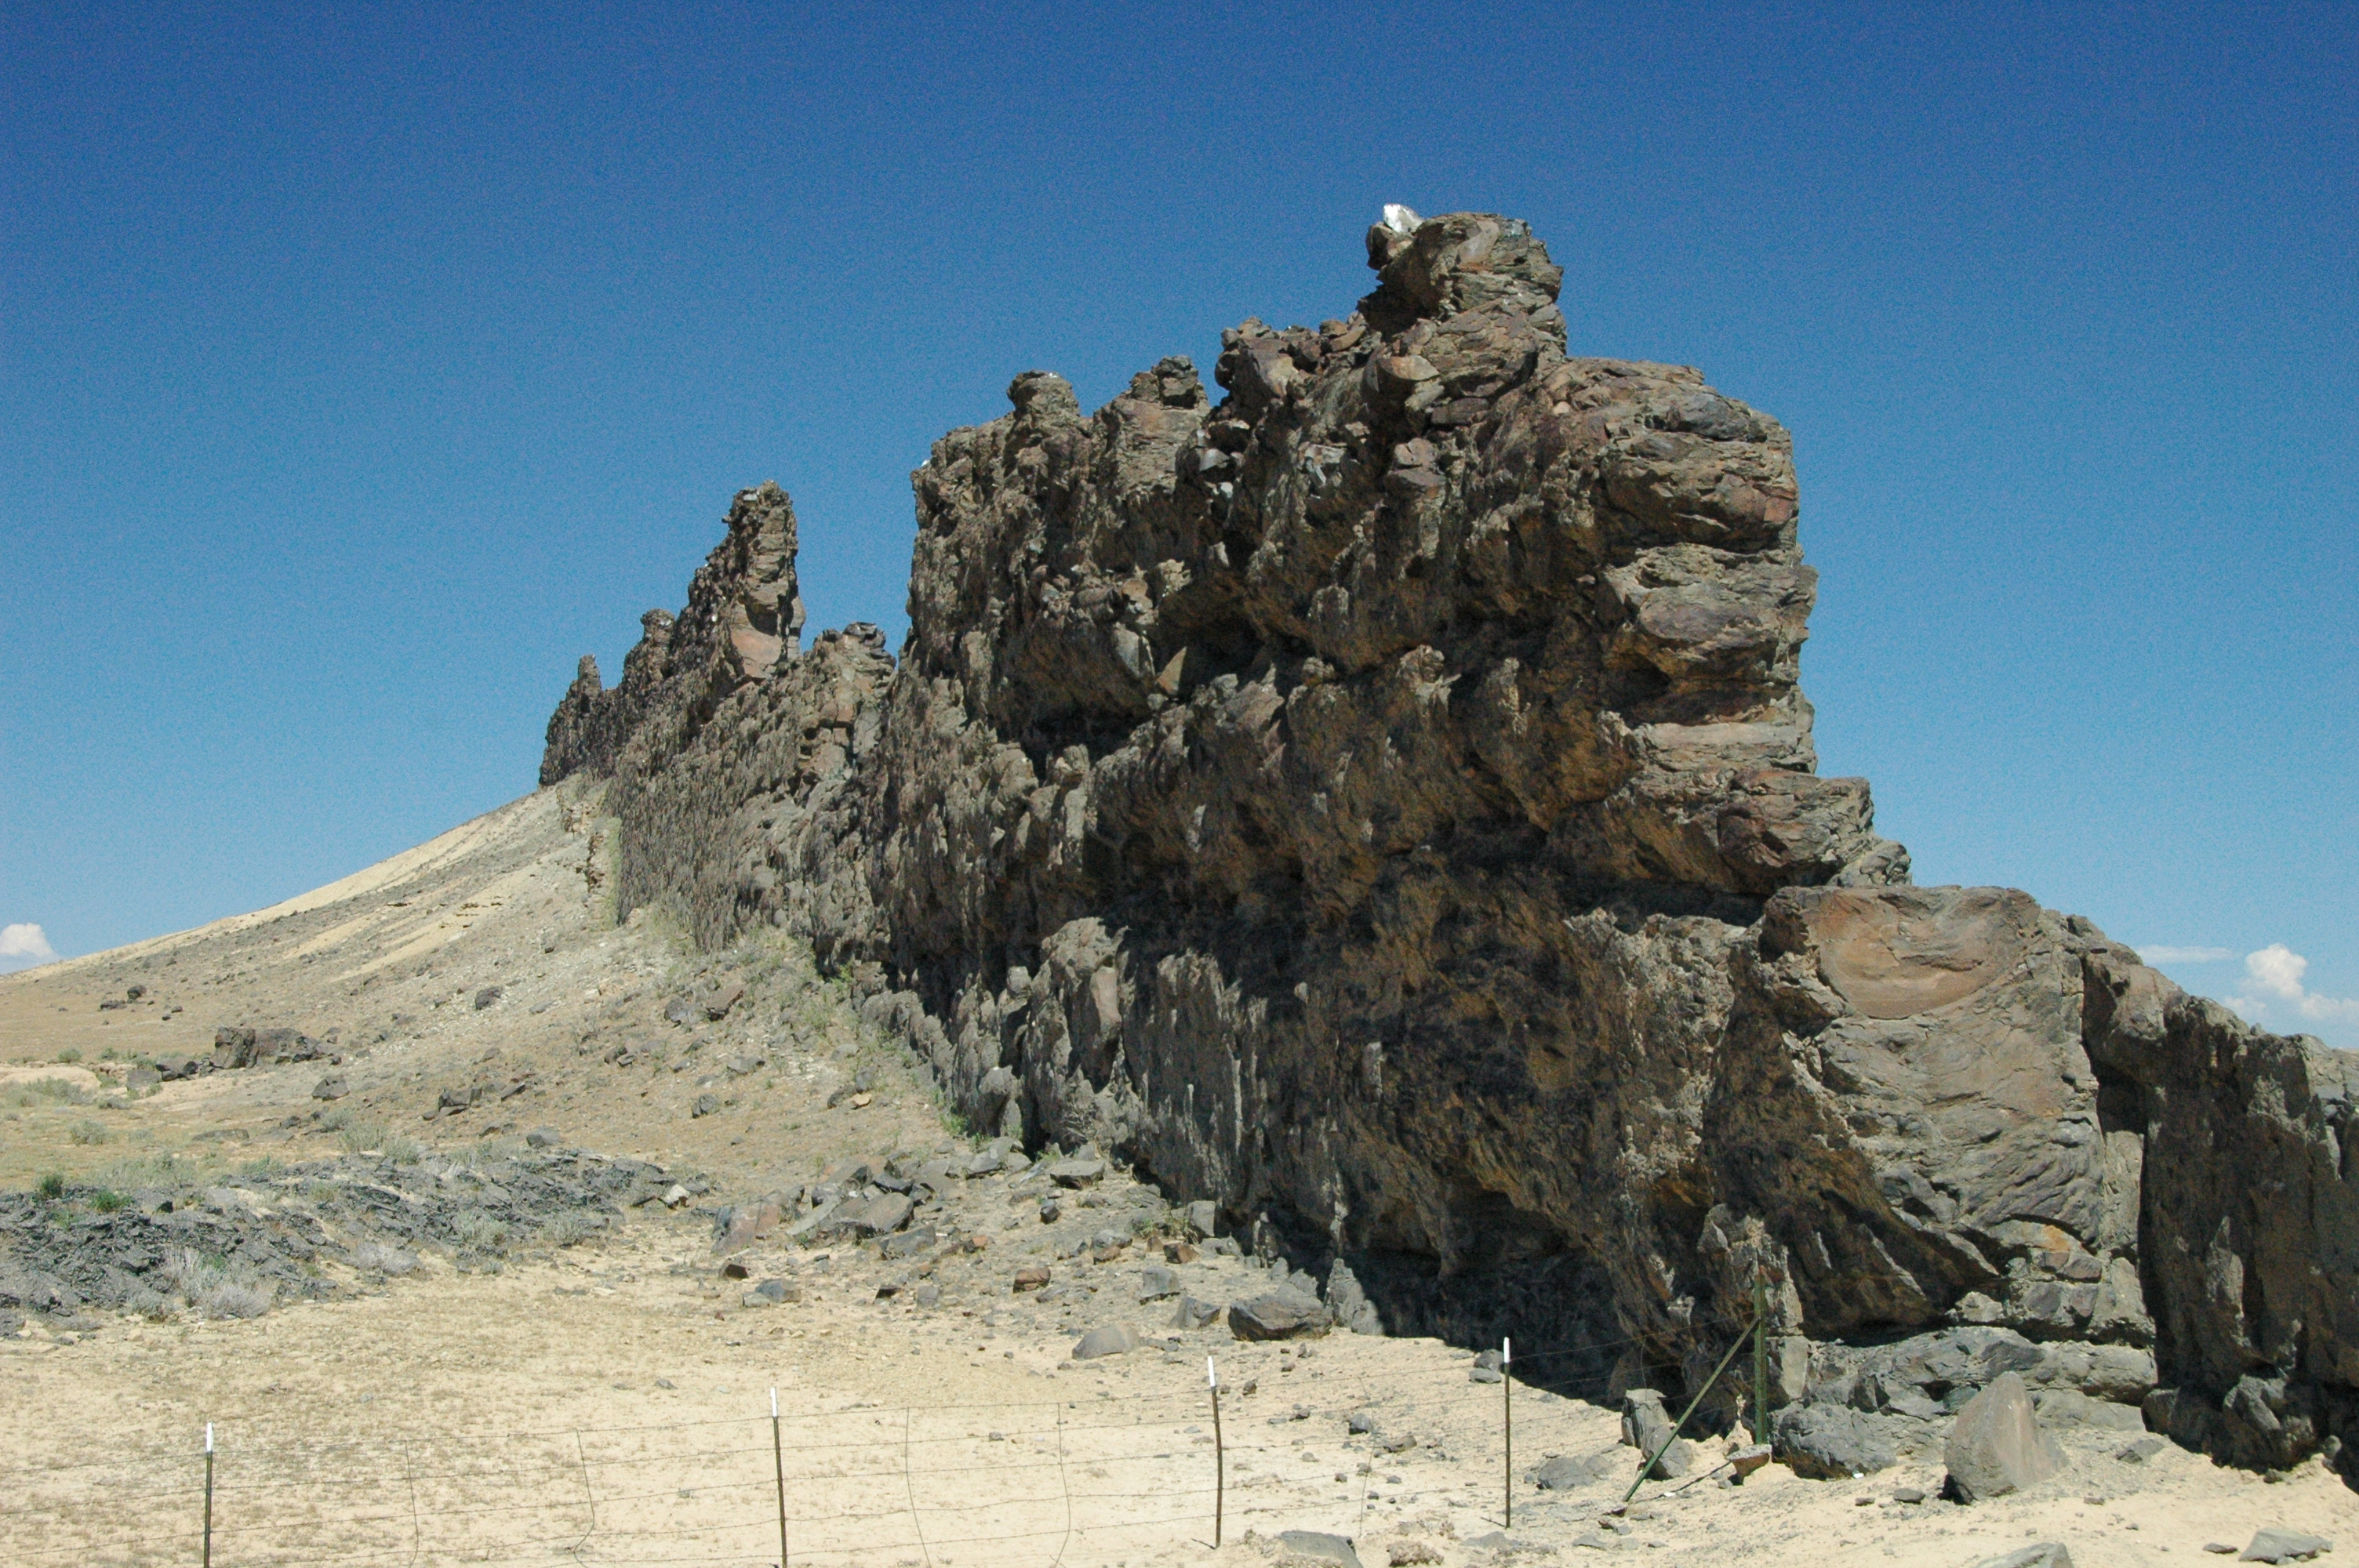
\includegraphics[width=1\linewidth]{obrazky/sopky/zila}
	\caption{Pravá žíla tvořená lamprofyrem. Stará 27-32 miliónu let. (Navajo Volcanic Field, New Mexico, USA). (Zdroj: James St. John https://www.flickr.com/people/jsjgeology/, CC BY 2.0, via Wikimedia Commons)}
	\label{fig:zila}
\end{figure}


\textbf{Ložní žíla} je konkordantní tabulové těleso o typické mocnosti \SIrange{10}{30}{\metre}. \textbf{Lakolit} je forma ložní žíly u které narostla její mocnost a vznikla tak klenba, což způsobilo i vyklenutí nadložních vrstev.

\begin{figure}[h]
	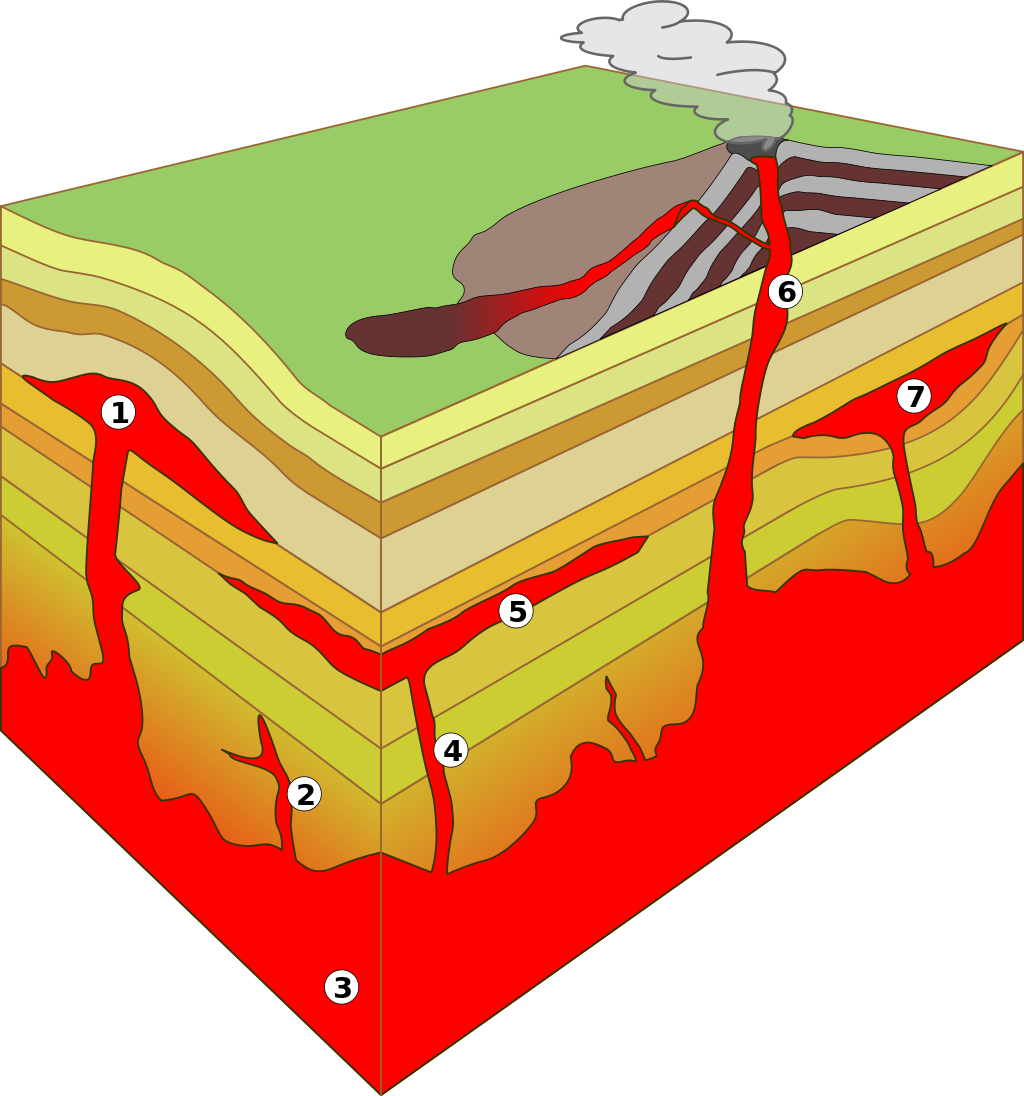
\includegraphics[width=\linewidth]{obrazky/sopky/Intrusion_types}
	\caption{Základní typy intruzí: 1. lakolit, 2. malá žíla, 3. batolit, 4. pravá žíla, 5. ložní žíla, 6. sopouch, 7. lopolit (Zdroj: Motilla, CC BY-SA 3.0 via Wikimedia Commons)}
	\label{fig:intrusion}
\end{figure}

\section{Sopky}
\subsection{Rozložení sopečné činnosti}

Sopečná činnost není rozložená rovnoměrně po zemském povrchu, ale je soustředěna hlavně na okraje litosférických desek a v místech horkých skvrn. V těchto oblastech je tak dominantním reliéfotvorným činitelem. V současné době ční nad hladinu světového oceánu okolo 600 sopek a to jak na kontinentech, tak v podobě sopečných ostrovů. Aktivních podmořských vulkánů je ale daleko víc. Udává se, že alespoň 50 000 se jich nachází na dně Tichého oceánu.

\subsection{Typy erupcí}
Podoba sopečné erupce je závislá na chemickém složení magmatu (zejména množství \ce{SiO2}), obsahu plynné složky a vody, jelikož ovlivňují jeho \textbf{viskozitu}. \emph{Kyselé (felsické) magma} (s velkým obsahem \ce{SiO2}) je viskózní, teče tedy pomalu. Neumožňuje snadný únik sopečných plynů, čímž se v sopce stupňuje tlak a často pak dochází k explozivním erupcím. Kyselá láva má malý prostorový dosah.

Málo viskózní \emph{basické (mafické) magma} (bazaltové), obsahuje cca jen 5 \% \ce{SiO2}. Materiál magmatu pochází z větších hloubek, zejména ze svrchního pláště. Toto magma je vázáno hlavně na riftové oblasti a horké skvrny. Erupce jsou mnohem klidnější. Dochází k výlevům magmatu na povrch. Díky malé viskozitě se láva roztéká do velkých ploch.

Vulkanické erupce se dělí do tří typů a to na \textbf{exhalační}, kdy do vzduchu unikají sopečné plyny. V případě, že dochází k výlevům lávy, tak je označována za \textbf{efuzivní}. V případě výbuchu hovoříme o \textbf{explozivním} typu vulkanické erupce. Do vzduchu je vyvrhován pevný materiál označovaný jako \textbf{tefra}.

\begin{table*}[]
	\setlength{\tabcolsep}{3pt}
	\footnotesize
	\begin{tabularx}{1\textwidth}{XXXXX}
		\toprule
		Typ erupce & Typ magmatu& Podoba výlevné aktivity& Podoba explozivní aktivity & Struktury a formy vytvořené okolo kráteru  \\ \midrule
		Islandská &	Basické, nízká viskozita &Rozsáhlé a silné výlevy z trhlin &Velice slabá &
		Velice rozsáhlé lávové kužely; lávové plošiny s tvorbou kuželů okolo trhlin v terminální fázi \\
		Havajská                    & Basické, nízká viskozita & Běžně tenké a rozsáhlé výlevy z centrálních sopouchů & Velice slabá & Velice rozsáhlé lávové dómy a štíty\\
		Strombolská &
		Střední viskozita; částečně kyselá, částečně bazická &
		Výlev chybí nebo jsou silné a středně rozsáhlé &
		Slabá až silná  &
		Struskové kužely a lávové proudy \\
		Vulkánská                   & Kyselé, viskózní        & Lávové proudy často chybí; případně o velké mocnosti         & Střední                      & Sypaný kužel; explozivní krátery \\
		Vesuviánská (silná Vulkánská) & Kyselé, viskózní        & Lávové proudy často chybí; silné                    & Střední až silné         & Sypaný kužel; explozivní krátery      \\
		Plinijská (extrémně silná Vulkánská) &
		Kyselé, viskózní &
		Proudy chybí; pokud jsou, tak různých mocností &
		Velice silné&
		Rozsáhlé sopečné pumy a lapilli; bežně žádná tvorba kuželun \\
		Pélejský &
		Kyselé, viskózní &
		Dómy a/nebo krátké, mocné proudy; mohou chybět &
		Podobně jako Vulkánský typ ale s nuees ardentes &
		dómy; kužely popela a prachu\\ \bottomrule
	\end{tabularx}
	\caption{Typy erupcí (upraveno podle \textcite{summerfieldGlobalGeomorphologyIntroduction1999a}).}
	\label{tab:erupce}
\end{table*}


\subsection{Sopečné produkty}

\subsubsection{Lávové proudy}
Magma, které se dostává na zemský povrch se označuje jako láva. Podoba lávy a formy, které tvoří jsou závislé na charakteru původního. Kyselé lávy jsou velice viskózní, což zmenšuje vzdálenost na kterou mohou dotéct. Málo viskozní, bazaltové lávy snadno tečou a dostávají se tak do značných vzdáleností od místa erupce. Dalším důležitým faktorem, který ovlivňuje rychlost tuhnutí lávy, když se dostane na povrch je také mocnost lávového proudu. 
\textbf{Pahoehoe} je láva s hladkým provazovitým povrchem, který vzniká vychladnutím tenké vrtstvy na povrchu a její následnou deformací tekoucí lávou pod povrchem. Pahoehoe vzniká z lávy o nízké viskozitě. Jejím chladnutím lávy a úbytkem plynů se viskozita zvyšuje a vzniká láva typu \textbf{aa}, jejíž povrch je rozeklaný a ostrohranný.


\begin{figure}[h]
	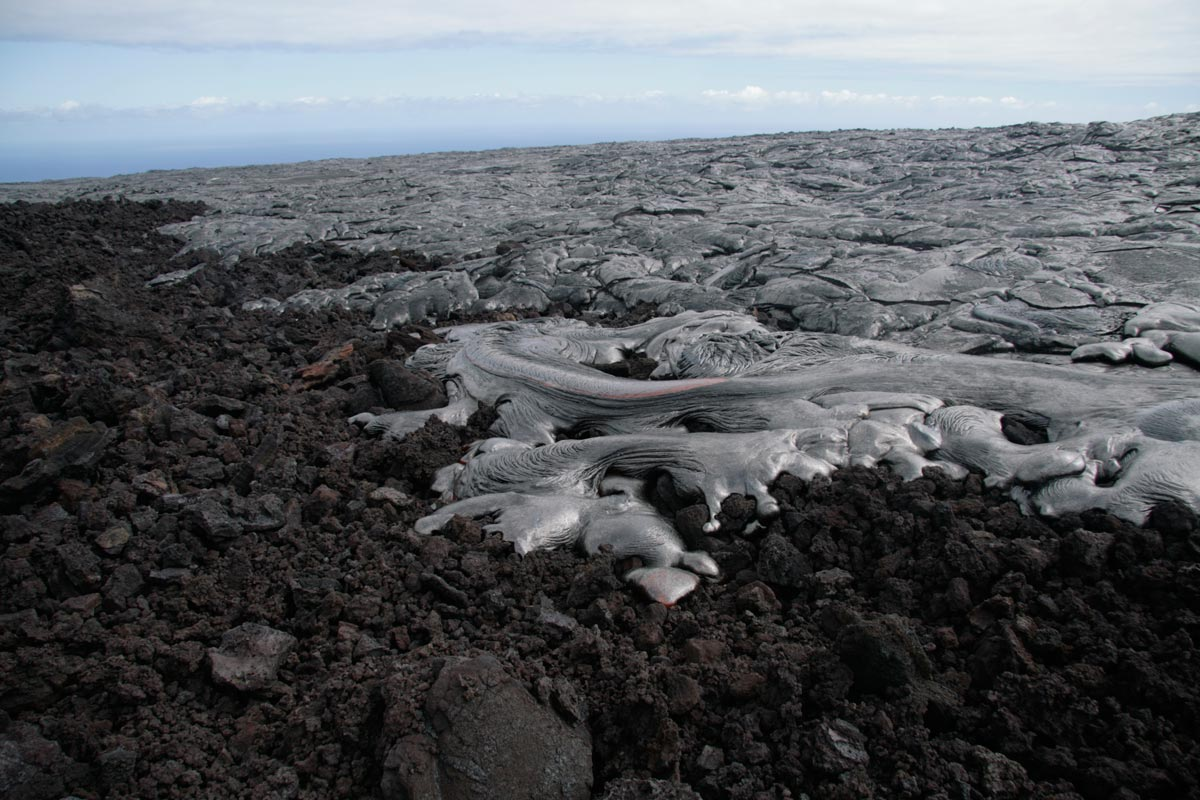
\includegraphics[width=\linewidth]{obrazky/sopky/paho_aa}
	\caption[Pahoehoe]{V popředí lávy typu aa, kterou překrývá láva pahoehoe. (Autor: USGS, veřejné dílo)}
	\label{fig:pahoe_aa}
\end{figure}

\subsubsection{Tefra}
Pyroklastický materiál, který sopky chrlí do okolí dělíme dle velikosti jednotlivých klastů. Nejjemnější je \textbf{sopečný popel}, kdy průměr částic je $<$ \SI{2}{\milli\metre}. Po zpevnění je nazýván tufem. Větší částice o průměru \SIrange{2}{64}{\milli\metre} nazýváme \textbf{lapilli}. Největší pyroklastika jsou \textbf{sopečné pumy} (průměr $>$ \SI{64}{\milli\metre} (obr. \ref{fig:puma}).

\begin{figure}[h]
	\centering
	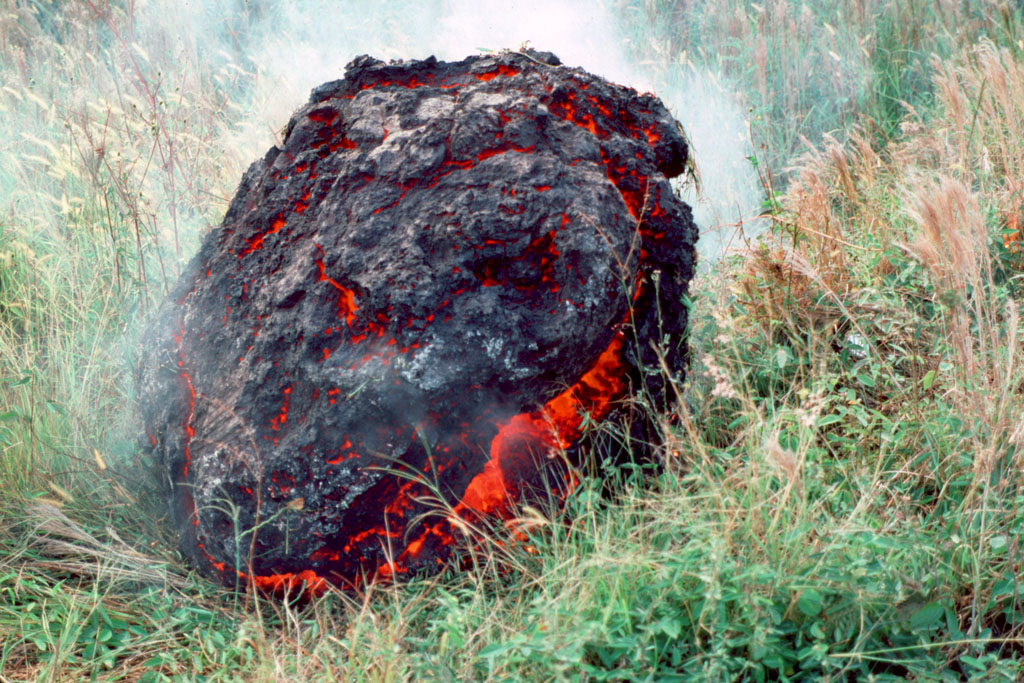
\includegraphics[width=1\linewidth]{obrazky/sopky/puma}
	\caption{Ještě žhavá sopečná puma vymrštěná ze sopky Kīlauea, Havaj (autor: J. D. Griggs, USGS, volné dílo)}
	\label{fig:puma}
\end{figure}


Zvláštním typem sopečného materiálu jsou \textbf{hyaloklastika}, která jsou spojená s erupcemi pod ledovcem. 

\subsubsection{Pyroklastický proud}
Pyroklastický proud (\textit{pyroclastic flow
}) je velice nebezpečný fenomén. Jedná se značně pohyblivou směs žhavých sopečných plynů a popela (obr. \ref{fig:pyroclastic}). Pohybuje se po sopečném svahu dolů rychlostmi, které se pohybují v rozmezí \SIrange{150}{700}{\kilo\metre\per\hour}. Teplota tekoucího materiálu je od \SIrange{100}{1100}{\celsius}.

\begin{figure}[h]
	\centering
	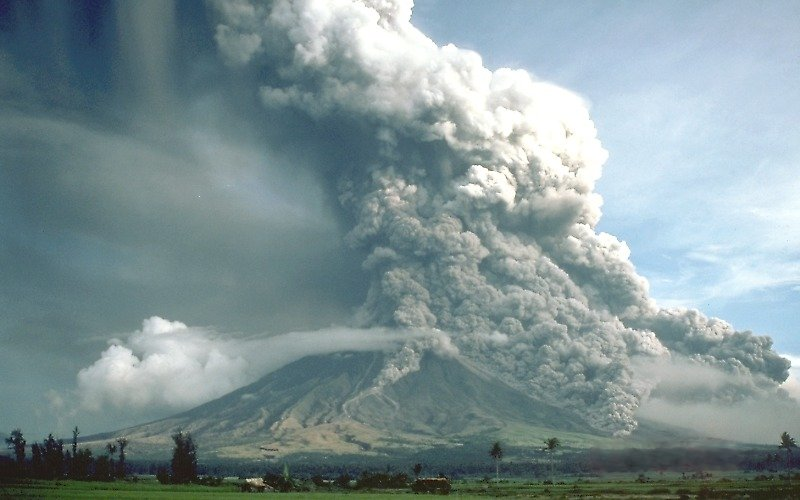
\includegraphics[width=1\linewidth]{obrazky/sopky/pyroclastic}
	\caption{Pyroklastické mračna tekoucá po úbočí sopky Mayon, Filipíny, 1984 (Autor:  C.G. Newhall, USGS)}
	\label{fig:pyroclastic}
\end{figure}


\subsection{Typy sopek}
\emph{Sypaný kužel} (tufová sopka) má podobu kužele s kráterem uprostřed, který je tvořena sopečným popelem,  struskou. Výška sypaných kuželů je zpravidla do \SI{300}{\metre}. Sypané kužely se často vyskytují ve skupinách případně v podobě parazitických sopouchů. Sypané kužely vznikají rychle (během jedné erupce -- monogenetické). 

\emph{Extruzinví sopky} neboli výtlačné kupy vznikají intruzí lávy. Kupy vzniklé vytlačením na povrch z kráteru se označují jako \emph{hornitos}. Složité výtlačné kupy, které vnzikají jako intruzivní klenby a následně roztaví nadloží se nazývají \emph{tholoidy}.

\emph{Maary} (Obr. \ref{fig:maar}) jsou malé a mělké krátery. Vznikají silnými explozemi při nadměrné produkci plynů. Mají většinou konkávní formu s nízkým obvodovým lemem ze sopečného popela. Často bývají vyplněné jezery.

\begin{figure}[h]
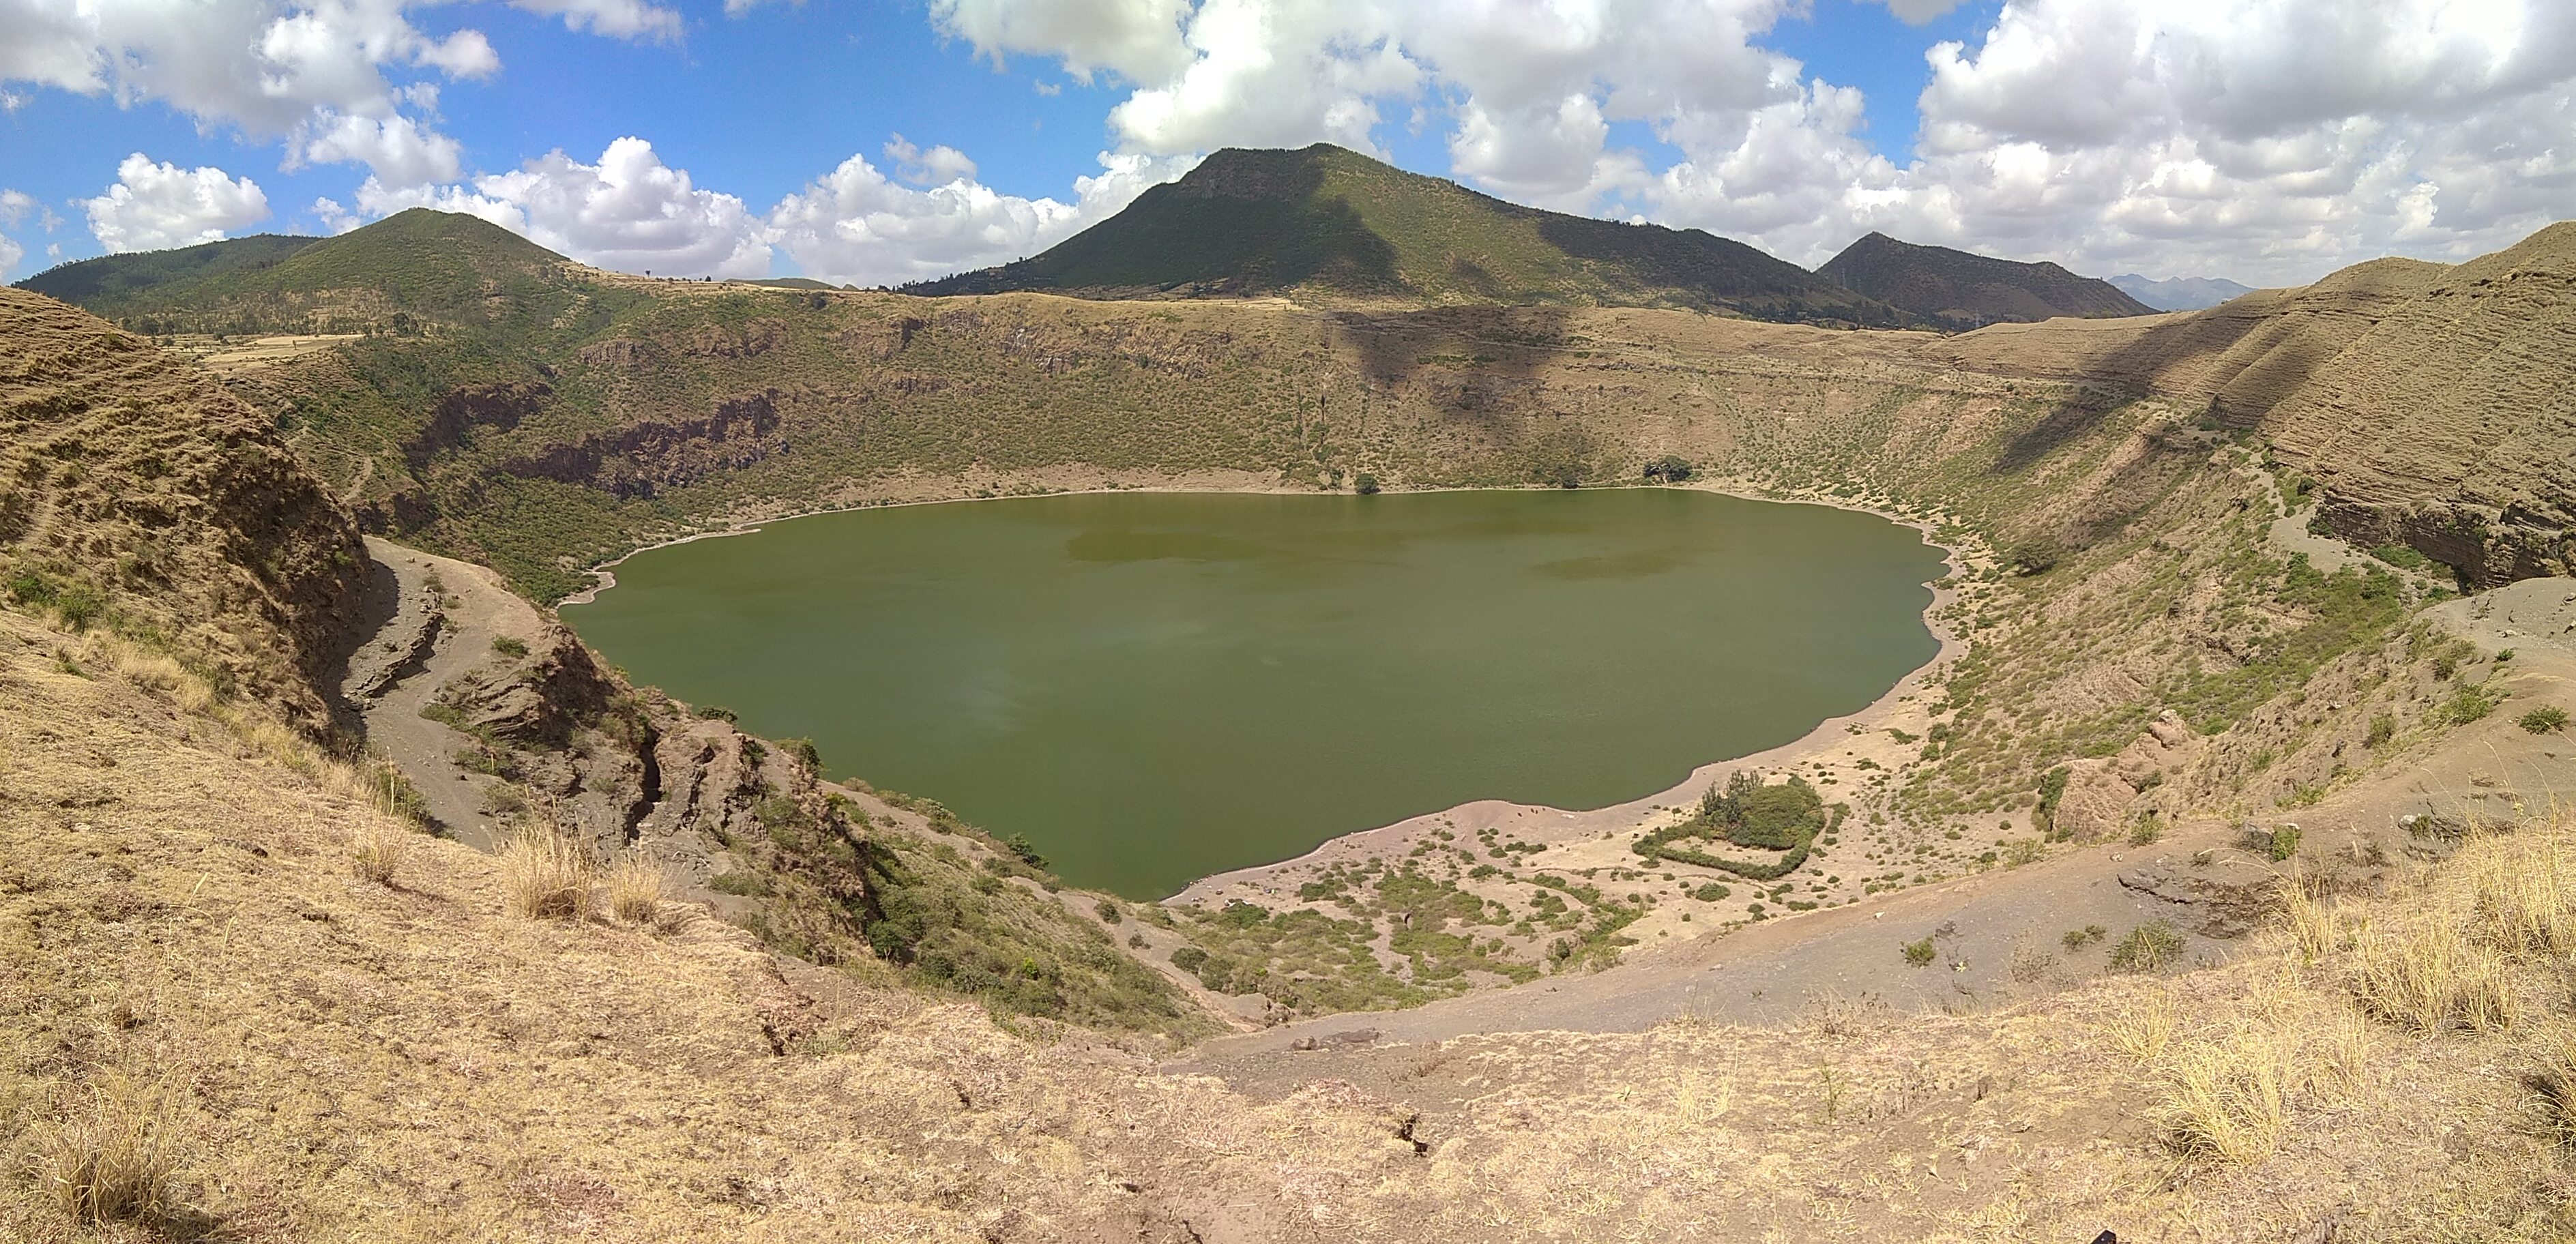
\includegraphics[width=\linewidth]{obrazky/sopky/maar}
\caption{Maar v oblasti Debre Zeit, Etiopie, Východoafrická riftová zóna (Autor: Giacomo Corti (distributed via imaggeo.egu.eu).}
\label{fig:maar}
\end{figure}

\emph{Stratovulkány} jsou nejběžnějším typem sopky. Je to smíšená sopka. Kužel stratovulkánu je tvořen ze střídajících se vrstev lávy a tefry (obr. \ref{fig:stratovulkan_rez}). Stratovulkány jsou tedy polygenetické. Na svazích se často nachází parazitické krátery. Pak hovoříme o tzv. složených stratovulkánech. 

\begin{figure}[h]
	\centering
	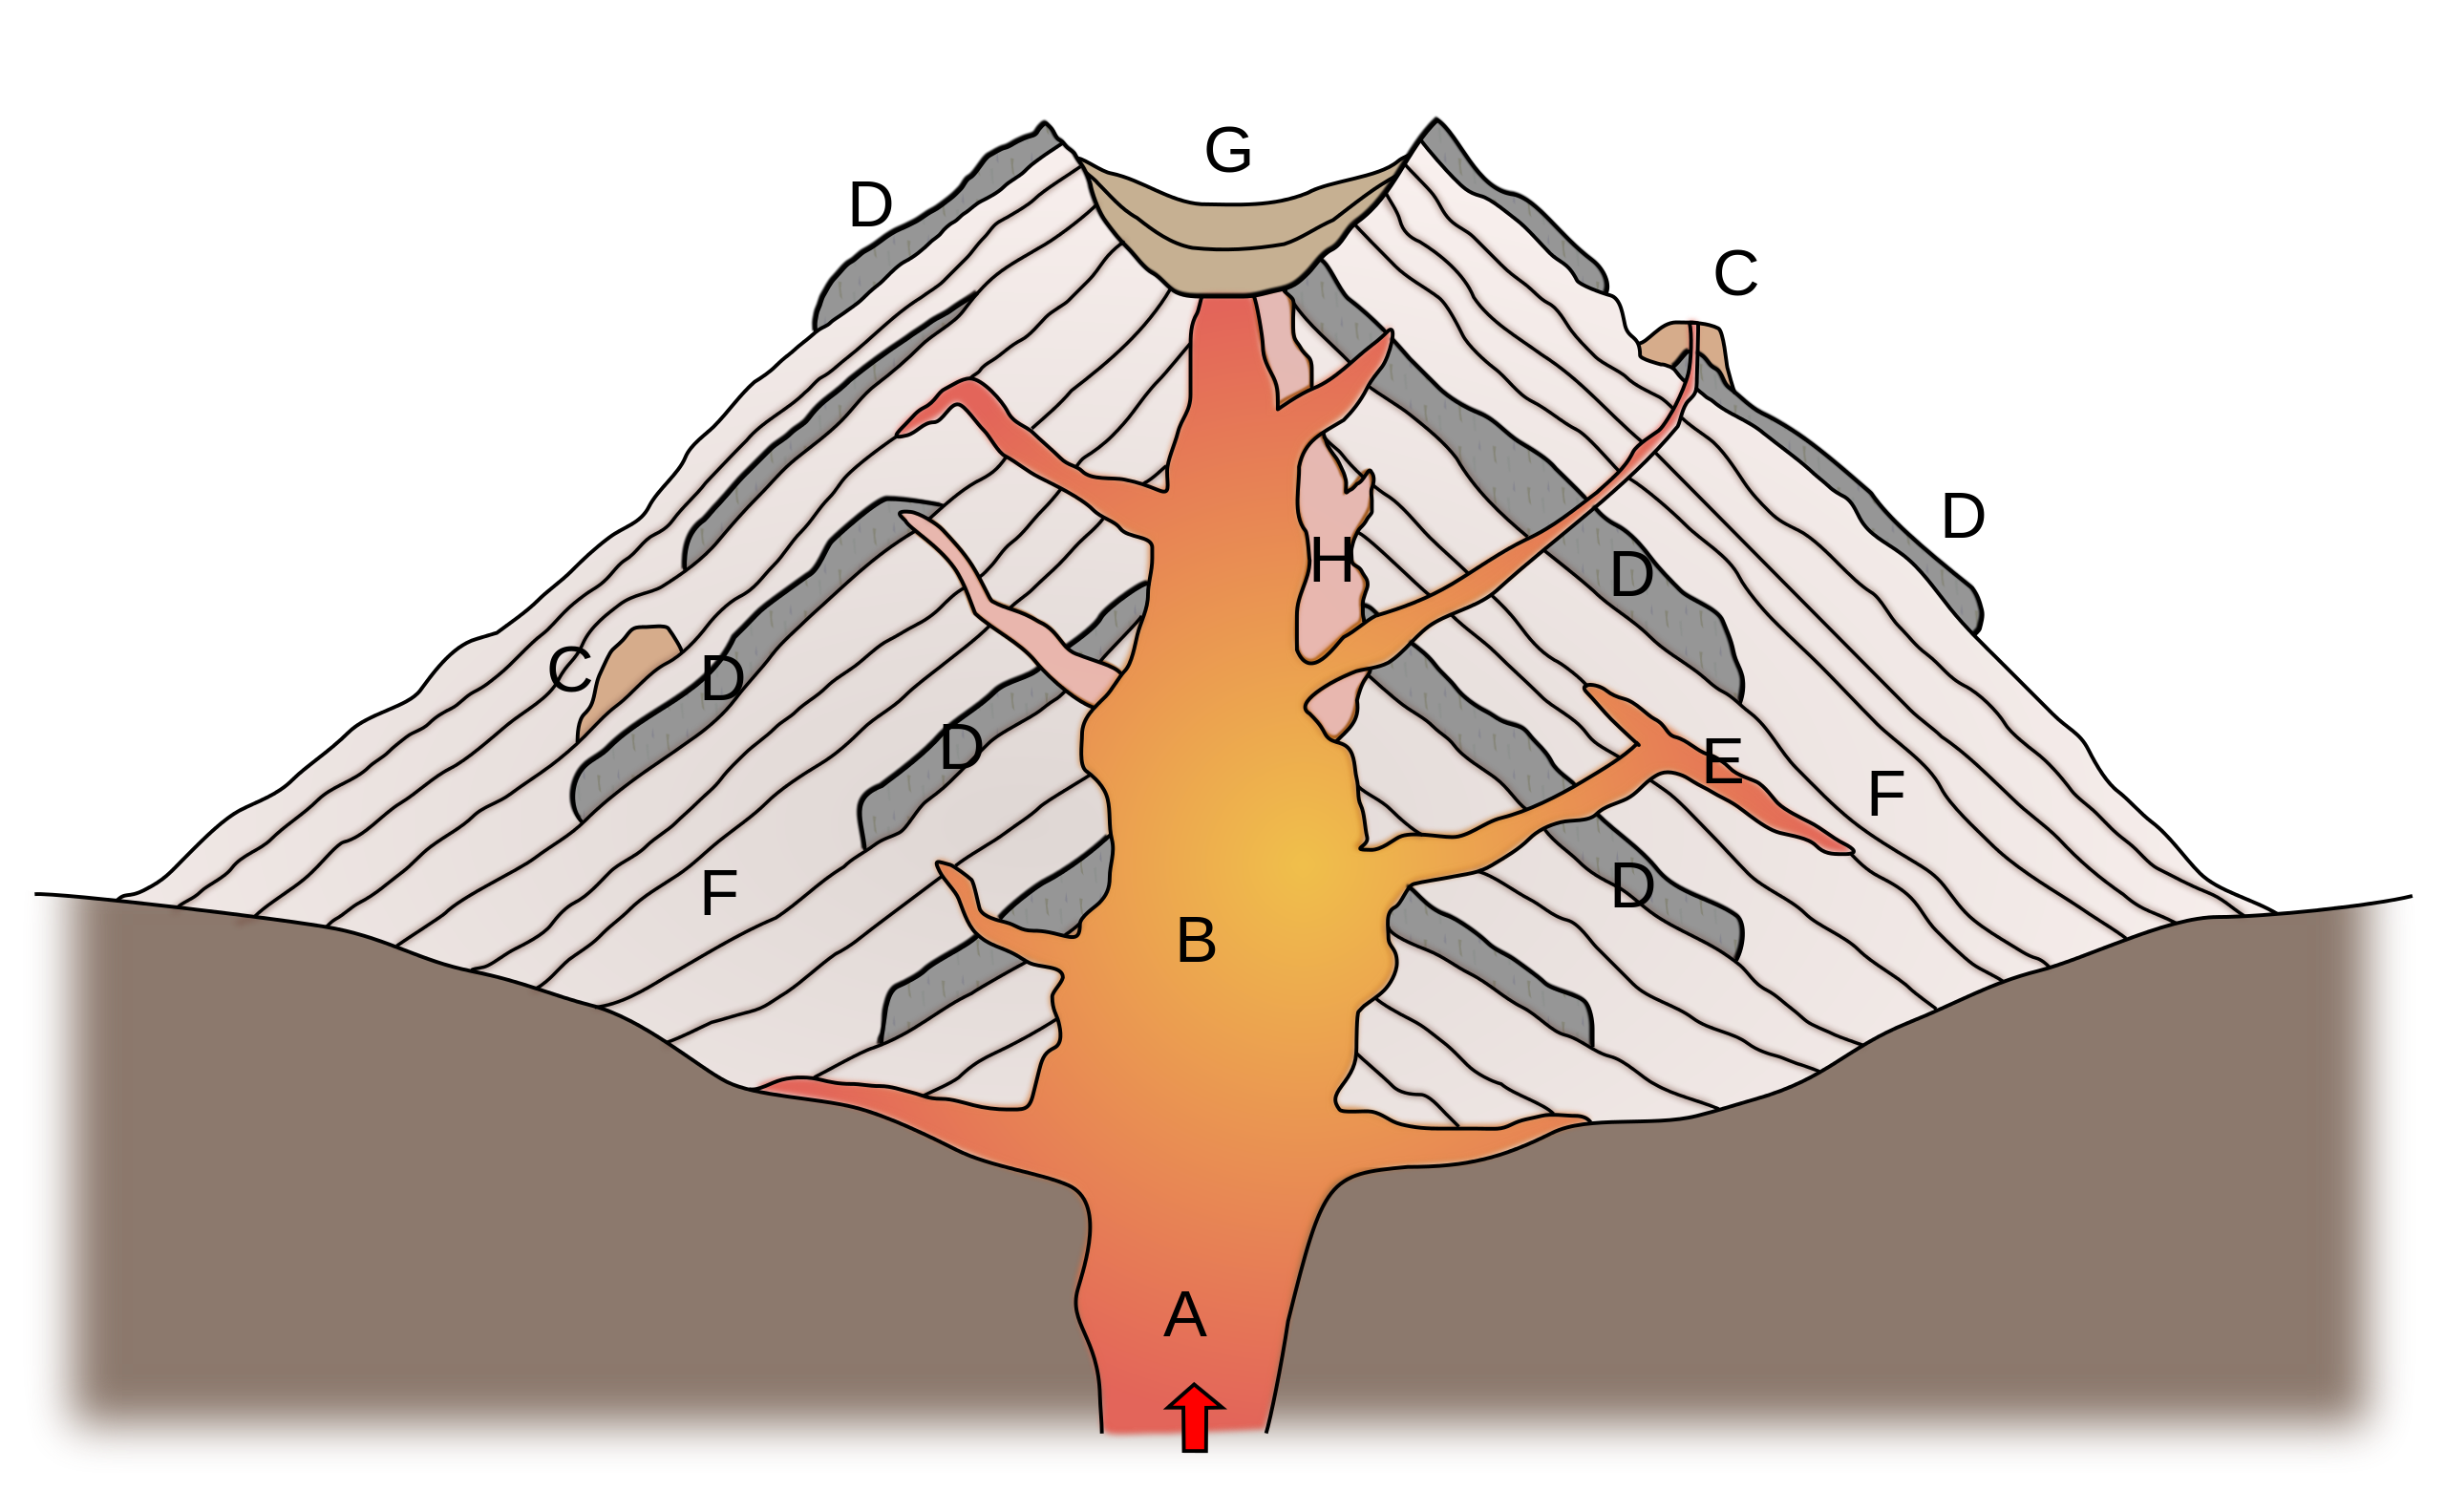
\includegraphics[width=1\linewidth]{obrazky/sopky/Stratovolcano_cross-section.svg}
	\caption{Schematický řez stratovulkánem. A: magma stoupá z magmatického krbu centrálním sopečným komínem (B); C: parazitický kráter a pyroklastický kužel na svahu stratovulkánu; D: lávový proud; E: ložní (nepravá) žíla; F: akumulace pyroklastik; G: kráter a jeho výplnň; H: starý komín (Autor: Woudloper, CC BY-SA 3.0, via Wikimedia Commons)}
	\label{fig:stratovulkan_rez}
\end{figure}




\begin{figure}[h]
	\centering
	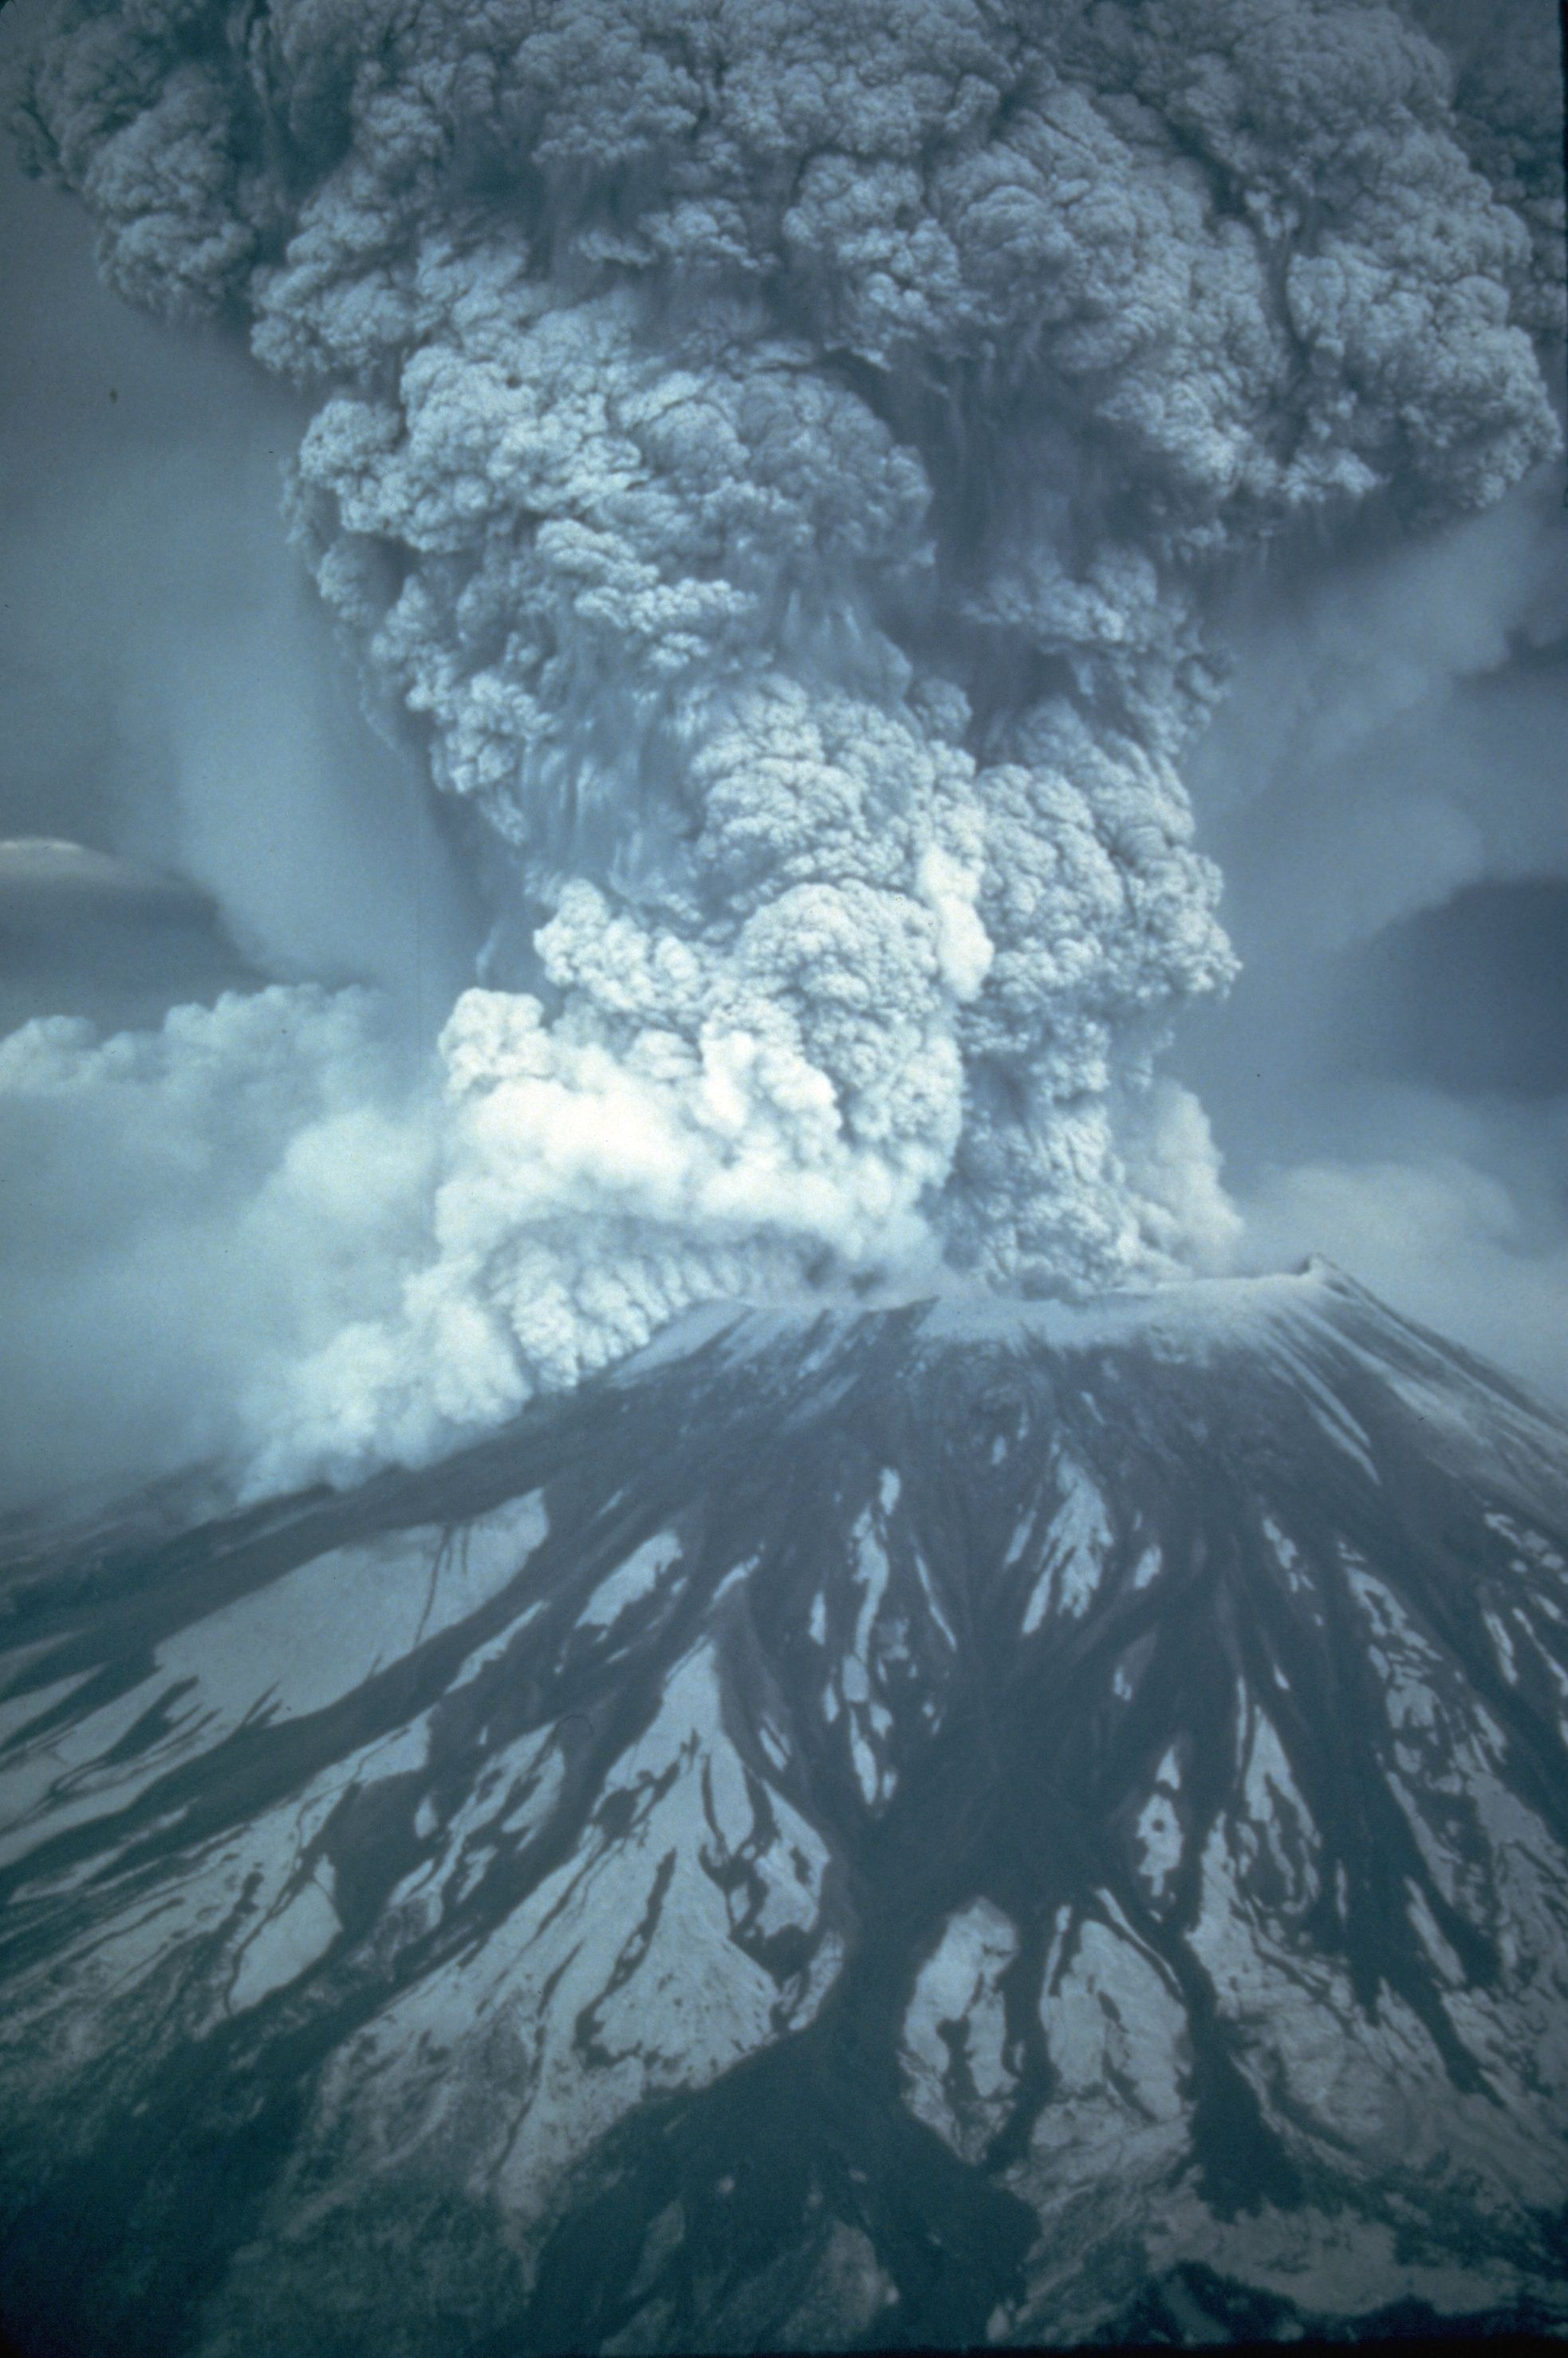
\includegraphics[width=\linewidth]{obrazky/sopky/st_helen}
	\caption{Výbuch sopky Sv. Helena (Autor: Austin Post, volné dílo)}
	\label{fig:sthelen}
\end{figure}

Vůbec nejrozsáhlejší vulkanickou formou jsou \textbf{štítové sopky}. Mohou nabývat dvou forem: centrální sopka s jedním kráterem kruhového charakteru. Druhá podoba je lineární sopka (tzv. eldgjá). Štítové sopky mají širokou základnu, sklon svahů je velice mírný (většinou $<$\SI{10}{\degree}). Dosahují ale velkých nadmořských výšek. Největší štítové sopky na Zemi lze nalézt na Havaji. Mauna Loa (obr. \ref{fig:maunaloa}) a Mauna Kea dosahují výšky \SI{4000}{\metre} nad mořem. Avšak jejich základna o šířce přes \SI{200}{\kilo\metre} se nachází v hloubce více jak \SI{5000}{\metre}. Největší štítová sopka ve Sluneční soustavě se nachází ale na Marsu. Olympus Mons ční do výšky \SI{26}{\kilo\metre}

\begin{figure*}[h]
	\centering
	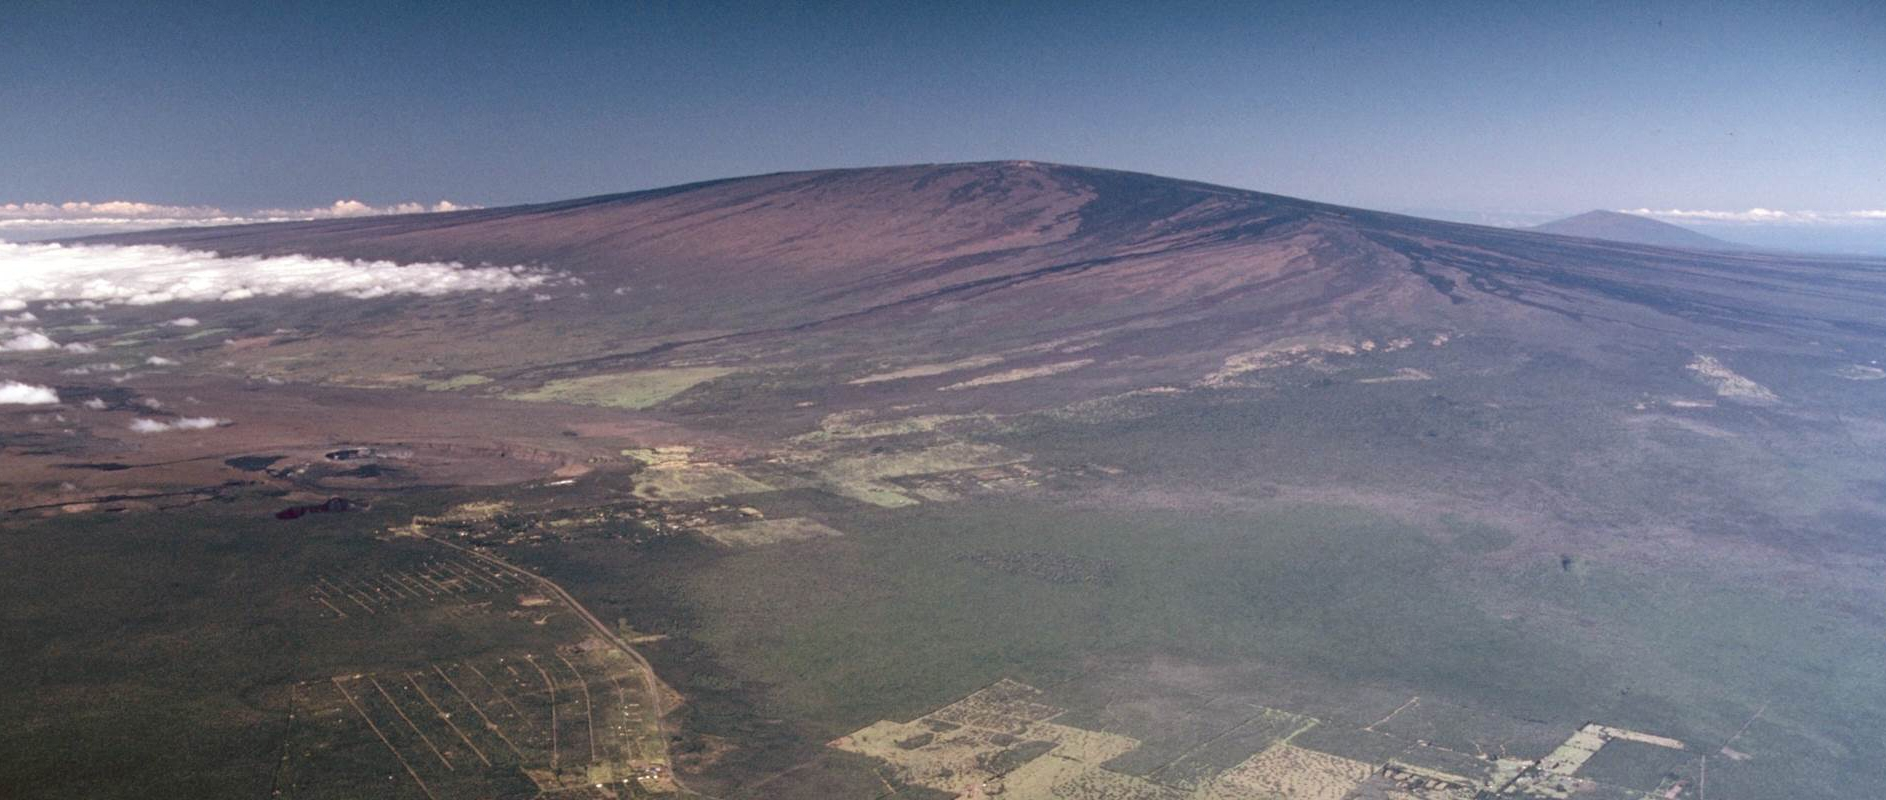
\includegraphics[width =1\textwidth]{obrazky/sopky/mauna_loa}
	\caption{Štítová sopka Mauna Loa, největší aktivní sopka na Zemi. Fotografie z roku 1985the largest active volcano on Earth. (Credit: J.D. Griggs, USGS, volné dílo)}
	\label{fig:maunaloa}
\end{figure*}

\textbf{Kaldery} jsou rozsáhlé krátery, které jsou geneticky spojené s vulkanismem. Dělíme je na explozivní -- vzniklé výbuchem již existujícího vulkánu a subsidenční, které vznikly poklesem povrchu nad vyprázdněným magmatickým krbem. 

\begin{figure*}[h]
	\centering
	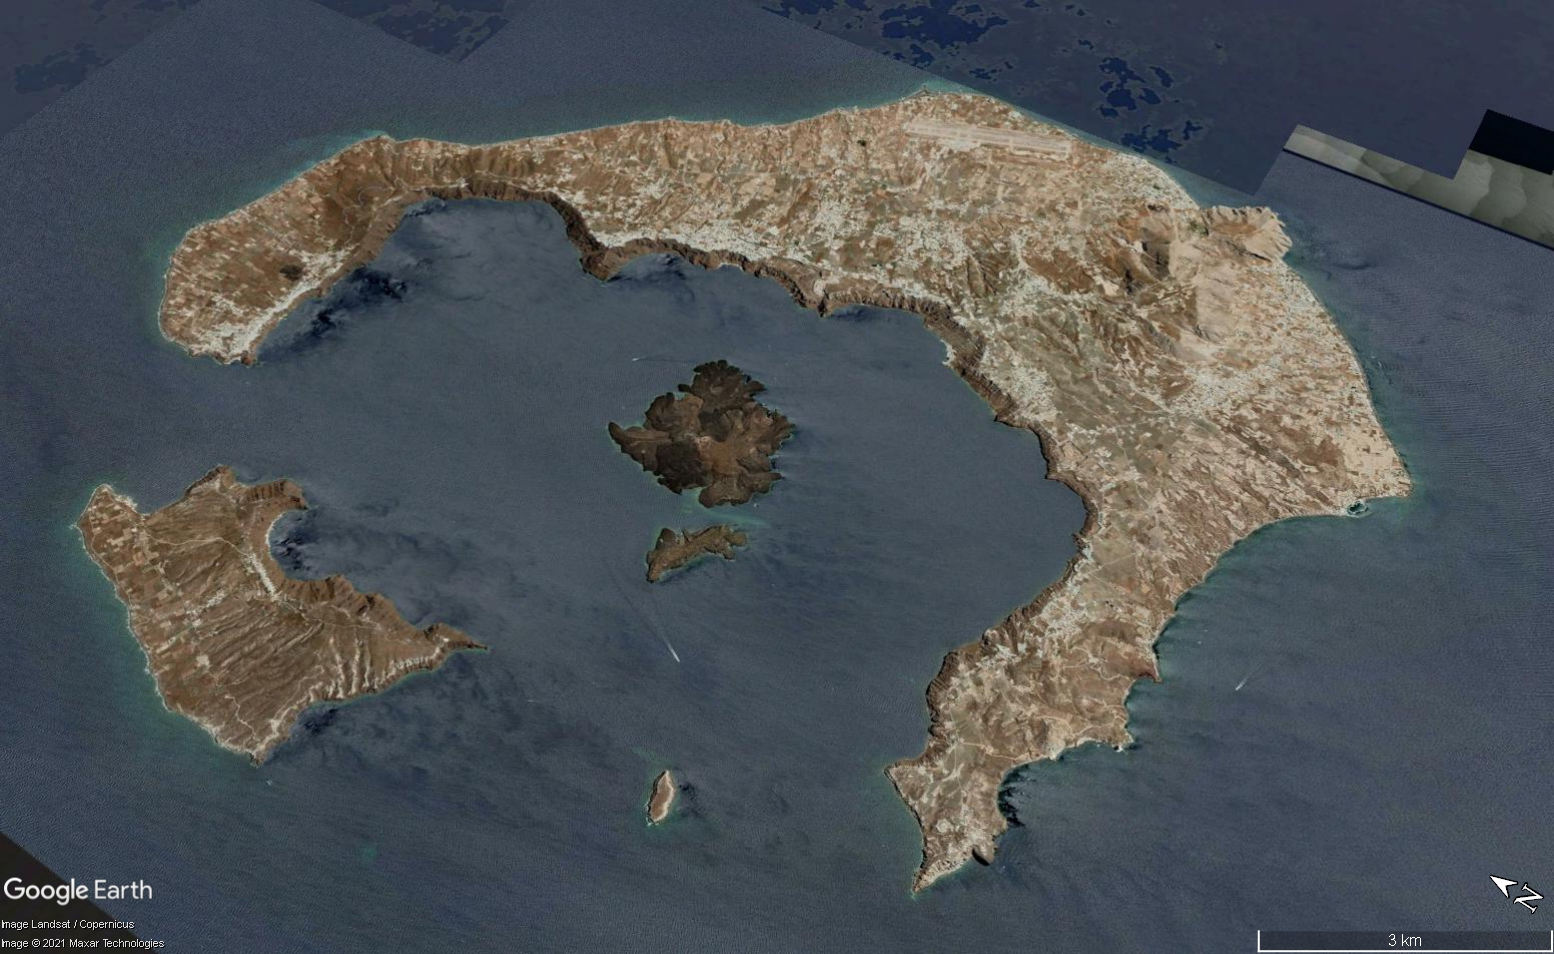
\includegraphics[width =\linewidth]{obrazky/sopky/santorini}
	\caption{Sopečná kaldera, ostrov Santorini, Řecko (Google Earth)}
	\label{fig:santorini}
\end{figure*}

\textbf{Trappy} jsou lávové pokryvy, které pokrývají rozsáhlé oblasti v plochém terénu. Známé jsou tzv. Dekkánské trapy v západní Indii (Obr. \ref{fig:trapy}), které jsou jedním z nejrozsáhlejších vulkanických těles na světě. V současné době je jejich plocha přibližně \SI{500000}{\kilo\metre\squared}. 

\begin{figure*}[h]
	\centering
	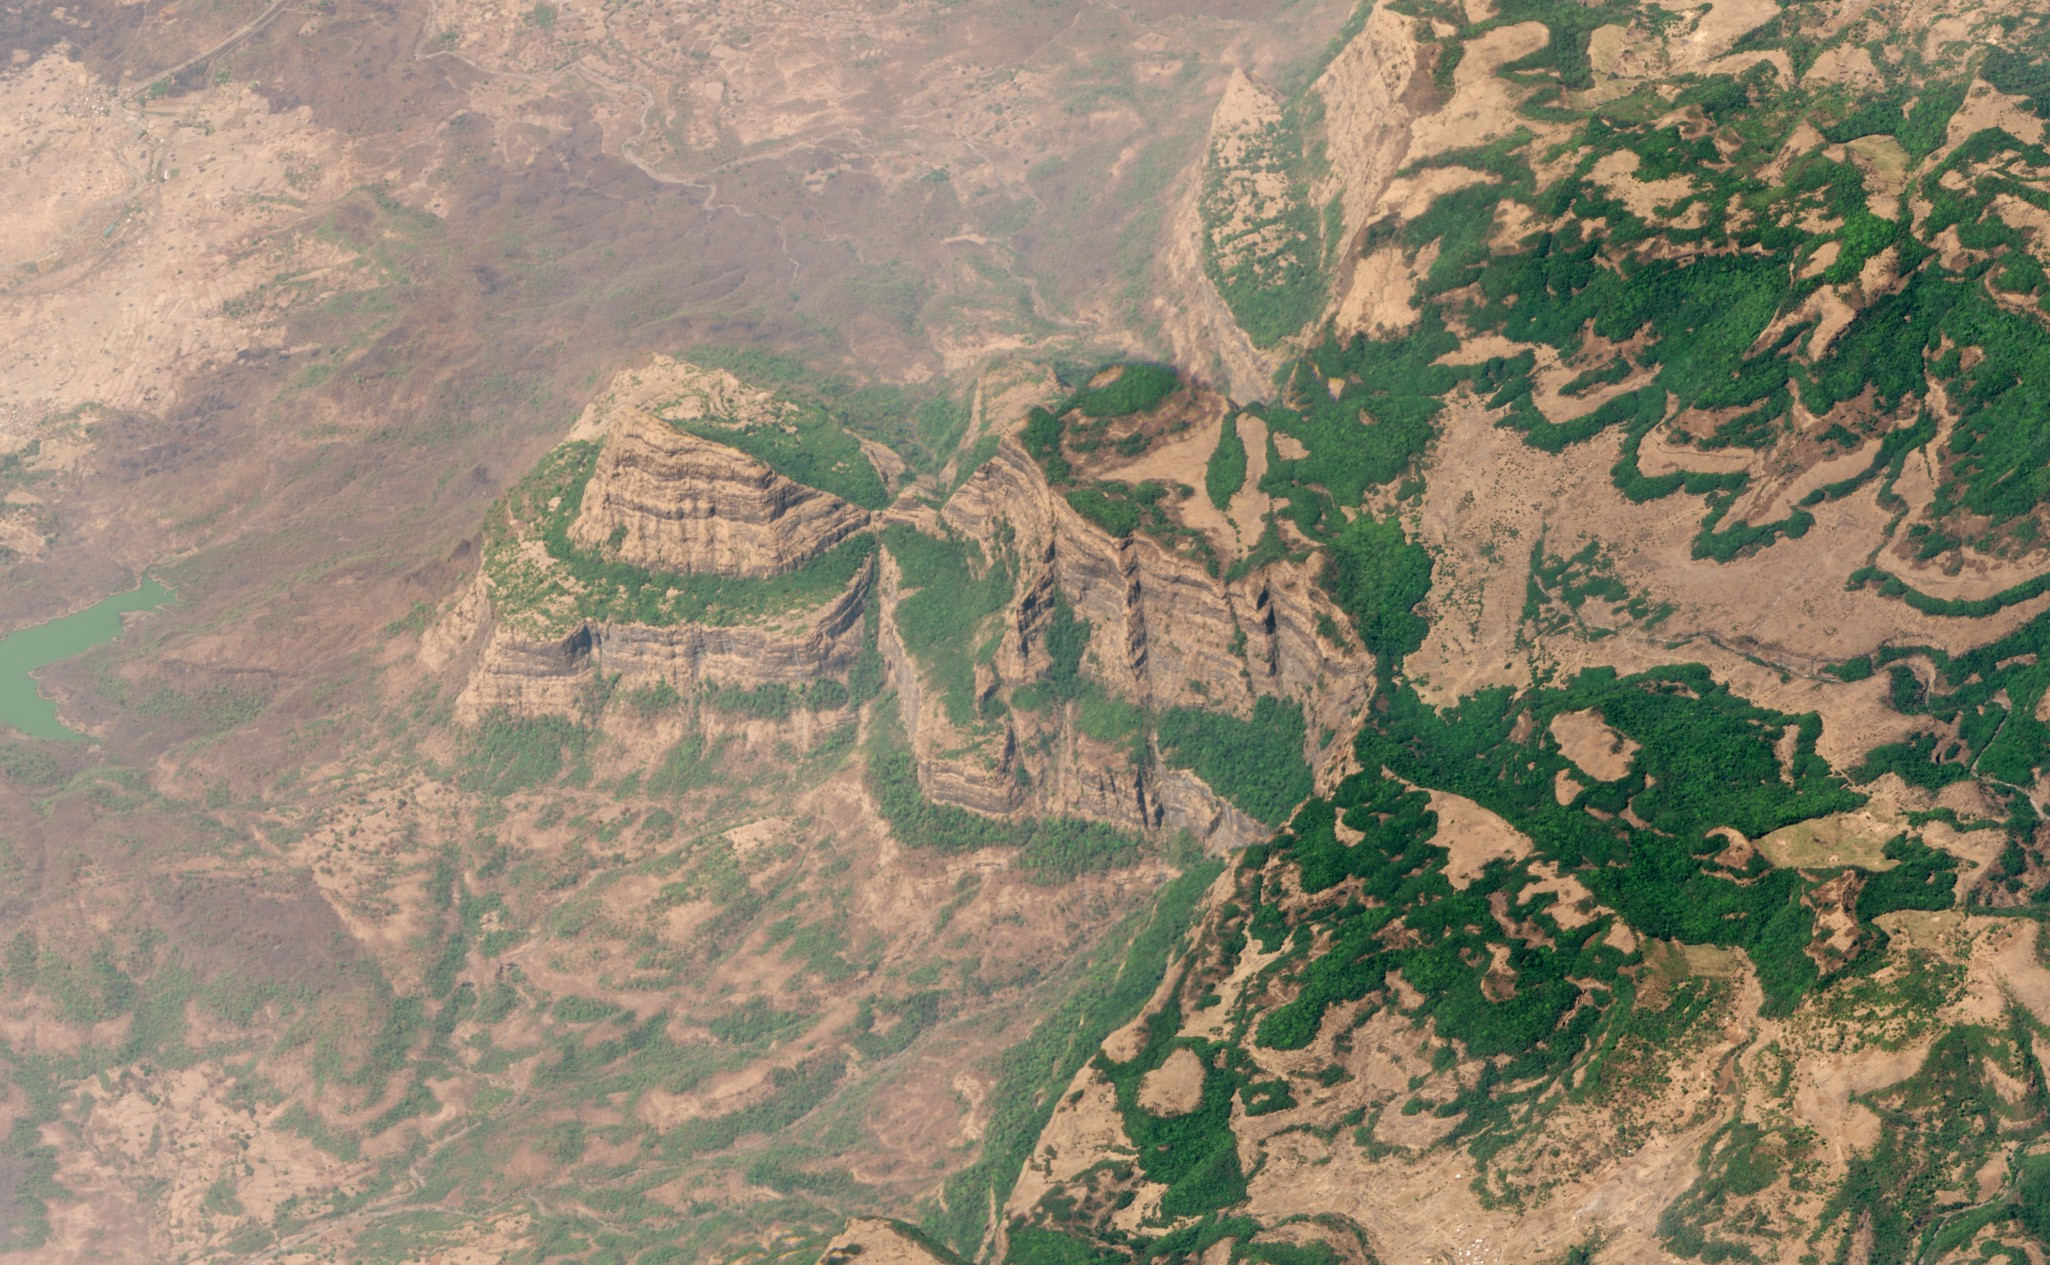
\includegraphics[width=\linewidth]{obrazky/sopky/trapy}
	\caption{Dekkánské trapy (zdroj: By Planet Labs, Inc - \url{https://medium.com/planet-stories/earths-wonders-like-you-ve-never-seen-them-before-ac9e2f39aa56}, CC BY-SA 4.0)}
	\label{fig:trapy}
\end{figure*}


	%%%%%%%%%%%%%%%%%%%%%%
	\part{Exogenní procesy a formy reliéfu}

	\chapter{Zvětrávání}
	\section{Základní podstata zvětrávání}
Zvětrávání je změna fyzikálních a chemických vlastností hornin po jejich obnažení na zemském povrchu. Produktem \emph{zvětrávacích procesů} jsou \emph{zvětraliny}. Ke změnám vlastností hornin dochází z důvodu odlišných fyzikálně-chemických podmínek při vzniku horniny a na zemském povrchu. Čím odlišnější podmínky panovaly při vzniku dané horniny, tím náchylnější je ke zvětrávání. Maximální možný dosah zvětrávacích procesů se udává okolo \SI{1}{\kilo\metre} do hloubky. Zvětrávání hornin je přípravou pro další procesy.

\section{Fyzikální (mechanické) zvětrávání}
Při fyzikálním zvětrávání dochází k rozrušování horniny a rozpadu na menší částice. Mění se tedy fyzikální vlastnosti hornin a ne chemické složení. U některých typů fyzikálního zvětrávání dochází až k rozpadu na jednotlivá minerální zrna. Příčinou jsou vždy změny objemu v horninovém masivu

\subsection{Změny teplot}
Horniny a minerály jsou špatným vodičem tepla. Při oslunění skalního povrchu se tak během dne prohřeje jen pár svrchních centimetrů. Zároveň s růstem teploty horniny roste i její objem. Dramatické rozdíly mezi teplotou na povrchu a uvnitř tak způsobují pnutí v hornině, což vede k odlupování tenkých slupek hornin (tzv. \emph{deskvamace}). Rozdílná teplotní roztažnost minerálů může způsobit vypadávání jednotlivých minerálních zrna tzv. \emph{odzrňování}. Prudké zahřátí povrchu vlivem např. lesních požárů způsobuje \emph{termické pukání} hornin. Silné ochlazení může naopak vyvolat \emph{mrazové pukání}.

% TODO: \usepackage{graphicx} required
\begin{figure}
	\centering
	\includegraphics[width=1\linewidth]{obrazky/zvetravani/mrazove}
	\caption{Ukázka mrazového tříštění, Svalbard.}
	\label{fig:mrazove}
\end{figure}

\subsection{Fyzikální zvětrávání vlivem růstu krystalů}
Růst krystalů způsobuje objemové změny v horninách a jejich následné tříštění. Voda když zmrzne zvětší svůj objem o necelých $\SI{9,08}{\percent}$, což vede k postupnému rozšiřování puklin a tříštění hornin (\emph{gelivaci}). Prodkutem \emph{makrogelivace} jsou například kamenná moře. \emph{Mikrogelivace} způsobuje oddělování jednotlivých zrn horniny (produkt je kryopelit).


K tříštění hornin dochází i růstem krystalů soli z roztoků. \emph{Solné tříštění} se hlavně uplatňuje u pórovitých hornin (např. pískovců) v aridních či příbřežních oblastech.

Objemové změny krystalů mohou nastávat i z důvodu některých chemických změna (např. hydratace, dehydratace či oxidace).

\subsection{Fyzikální zvětrávání vlivem odlehčení (exfoliace)}
\emph{Exfoliace} je proces při kterém se z výchozů skalního podloží odlupují horninové slupky rovnoběžné s povrchem. Exfoliační pukliny vznikají z důvodu odlehčení hornin. Odstraněním nadloží se totiž v horninách uvolňuje napětí, které bylo indukované tíhou nadložních hornin. Nejčastěji jsou tyto pukliny při povrchu, avšak byly nalezeny i několik desítek metrů pod povrchem.
Mocnost exfoliačních slupek se zpravidla pohybuje od 0,5 do \SI{10}{\metre}, v takovém případě hovoříme o \emph{makroexfoliaci}. Odlupování tenčích slupek (v řádu \si{mm} až \si{cm}) označujeme jako \emph{mikroexfoliaci}.

Exfoliací vznikají exfoliační klenby. Nízké se nazývají \emph{ruwary}, vysoké \emph{bornhardty}.

% TODO: \usepackage{graphicx} required
\begin{figure}[h]
	\centering
	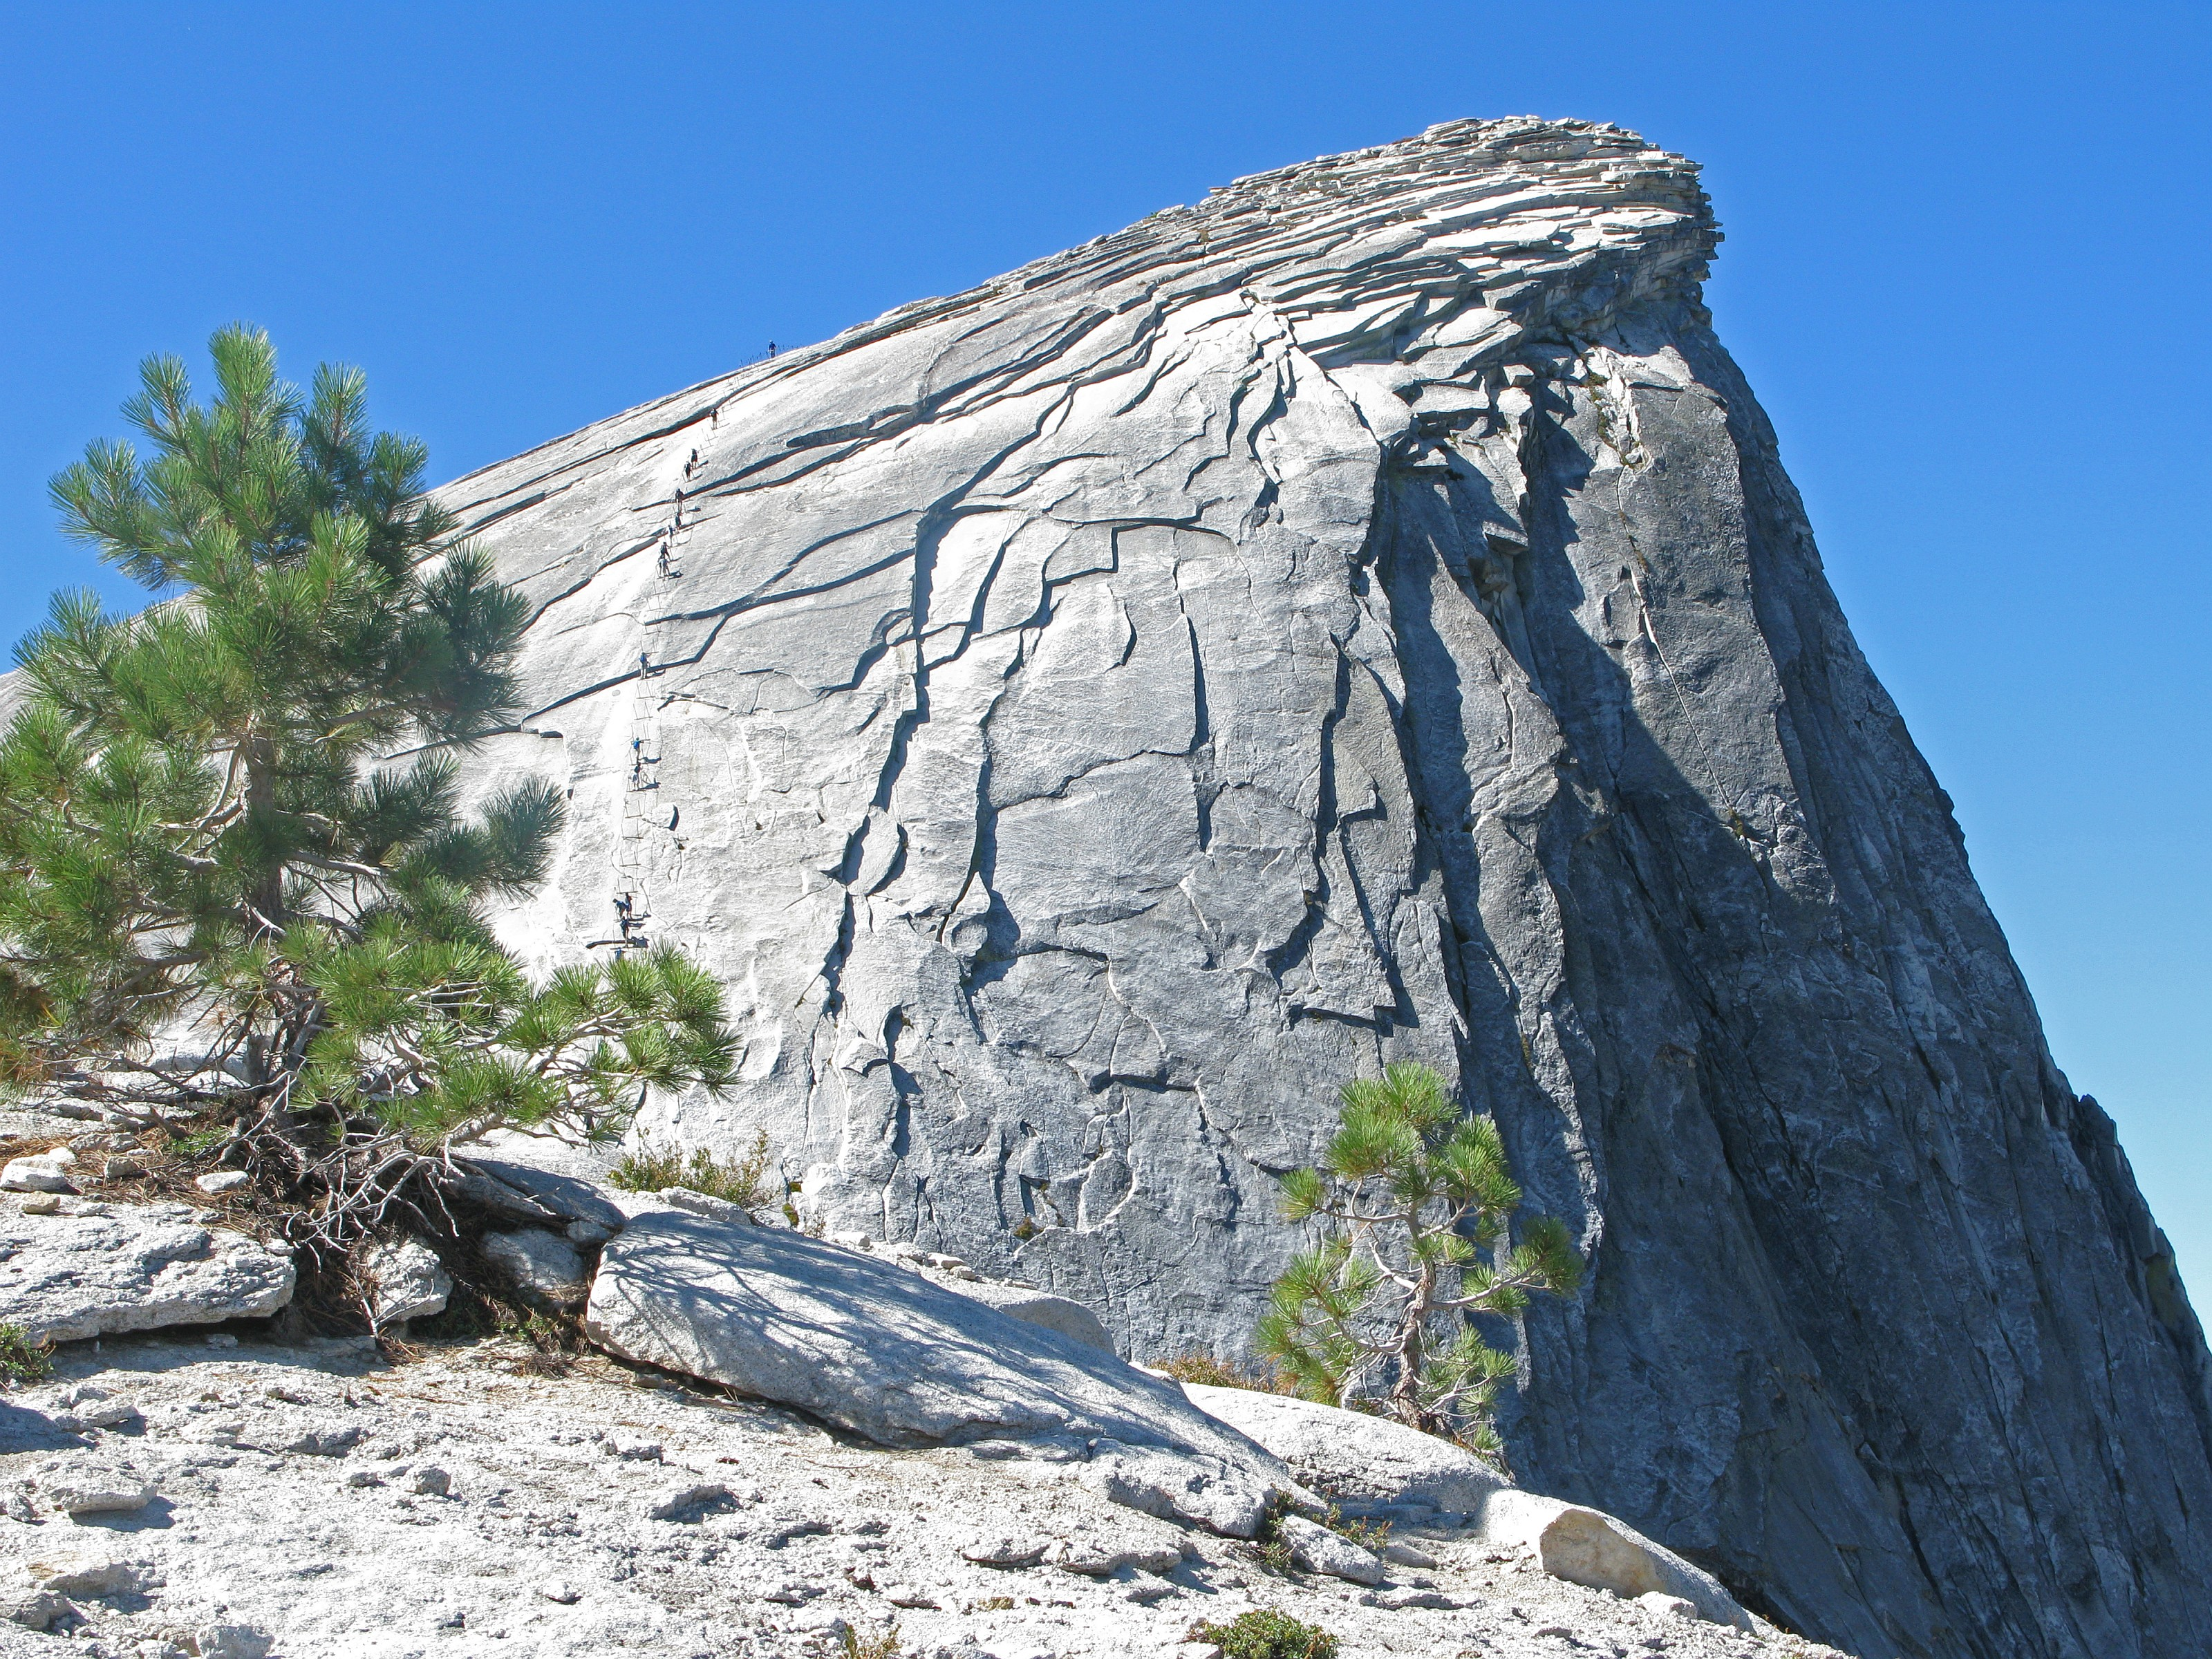
\includegraphics[width=1\linewidth]{obrazky/zvetravani/exfoliace}
	\caption{Ukázka exfoliace žuly. Half Dome v Yosemitském národním parku. (Autor: Ronnie Macdonald, CC BY 2.0 )}
	\label{fig:exfoliace}
\end{figure}


\section{Chemické zvětrávání}
\emph{Chemické zvětrávání} (také rozklad nebo dekompozice) je změna chemických vlastností hornin a jejich minerálů. Dochází k nahrazení stávajících minerálů jinými. Změna chemických vlastností je provázena i zvětšením objemu a zmenšením hustoty minerálů. Základní podmínkou pro chemické zvětrávání je \emph{přítomnost vody} a dostatečná \emph{teplota}.

Minerály, který vznikaly při podmínkách značně odlišných od těch co panují na zemském povrchu, zvětrávají rychleji, než ty které vznikaly za podmínek podobných. Tmavé (mafické) minerály zvětrávají na zemském povrchu rychleji než světlé (felsické) minerály. Tedfy olivín a pyroxen zvětrává rychleji než muskovit či dokonce křemen. Tzv. \emph{Goldichovo pravidlo zvětrávání} je v podstatě obráceným \emph{Bowenovým krystalizačním schématem}, které znázorňuje pořadí minerálů krystalizujících z postupně chladnoucího magmatu. Ty minerály, které krystalizují př nejvyšších teplotách naopak nejrychleji podléhají zvětrávání. Samozřejmě v přírodních podmínkách to je poněkud komplikovanější. 

Mobilita kationtů v minerálech ovlivňuje jak rychle se uvolní daný prvek z horniny, jak dlouho zůstává rozpuštěný ve vodě. Pořadí od nejmobilnějších k těm nejméně mobilným: \ce{Ca^2+, Na+, Mg^2+} $>$ \ce{K+} $>$ \ce{Fe^2+} $>$ \ce{Si^4+} $>$ \ce{Fe^3+} $>$ \ce{Al^3+}. Nejmobilnější kationy (\ce{Ca^2+, Na+, Mg^2+}) jsou první, které jsou z hornin vyplavovány. Naopak málo mobilní kationy ajko je \ce{Si^4+, Fe^3+, Al^3+} zůstávají ve zvětralině, kde dochází postupně ke zvyšování jejich koncentrace. 

\subsection{Typy chemického zvětrávání}
Nejjednodušším typem chemického zvětrávání je \emph{rozpouštění}. Rozpustnost minerálů je závislá na teplotě, pH a ale také i na rychlosti proudění vody v horninových pórech. Například dešťová voda je díky rozpuštěnému \ce{CO2} lehce kyselá (pH = 5,7). Významné je rozpouštění vápenců, které vede ke vzniku krasových oblastí a výzdob. 
%\subsubsection{Rozpouštění}
%Jedná se o nejjednodušší typ chemického zvětrávání. Rozpustnost minerálů je závislá na teplotě a pH vody.
%
%\subsubsection{Hydrolýza}

Dalším typem chemického zvětrávání je \emph{hydrolýza}. Ionty vody (\ce{H+} a \ce{OH-})  Molekula vody se dělí na proton (\ce{H+}) a hydroxidový aniont (\ce{OH-}). Vodíkový kation nahrazuje v krystalické mřížce kationy kovů (\ce{K+, Na+, Ca^2+, Mg^2+}) a ty se sluřují s hydroxidovým aniontem a stávají se součástí roztoku. Hydrolýza je hlavním procesem zvětrávání u silikátových hornin.

\emph{Oxidace} je typem reakce, při které prvek nebo sloučenina ztrácí jeden elektron (zvyšuje se tak jeho oxidační číslo). Například železnaté sloučeniny se oxidují na železité (\ce{Fe^2+} na \ce{Fe^3+}). Oxidačním činitelem nemusí být jen kyslík, ale například trojmocné železo, čtyřmocný mangan aj., zkrátka ty ionty, které jsou schopny přijmout elektron od oxidované sloučeniny. Oxidace je dominantní u minerálů, které obsahují \ce{Fe} (pyrit, siderit atd.), ale také \ce{Al}, \ce{Mg}, \ce{Mn}, \ce{Cr}. Opakem oxidace je \emph{redukce}. Redukovaná sloučenina přibírá elektron. Redukčním činitelem jsou ty ionty, které mohou elektrony předávat (např. dvojmocné železo, dvojmocný mangan). Projevy oxidace a redukce lze ve zvětralině či půdě poznat podle barvy. Hnědé či červené zbarvení poukazuje na oxidační prostředí, jelikož je typickým znakem oxidů trojmocného železa, kdežto šedá až šedozelená barva je typická pro redukční prostředí.


\emph{Hydratace} označuje proces obohacování minerálu vodou. Ta se dostává do krystalické mřížky. Sloučenina, která přijímá vodu, zvětšuje svůj objem a tím může mechanicky působit na své okolí. Opakem tohoto procesu je \emph{dehydratace}.

\emph{Karbonatizace} je reakce za účasti hydrogenuhličitanového anionu (\ce{HCO3^-}). Ten se nachází ve vodě v důsledku rozpoučtění \ce{CO2} ve vodě a následné disociace kyseliny uhličité (\ce{H2CO3}): 
\ce{H2O + CO2 <-> H2CO3 <-> H^+ + HCO3^-}
Karbonatizace je důležitá pro zvětrávání vápenců (reakce krasovění).

\emph{Lateritizace} je proces, který je vázán na monzunové vnější tropy, kde je vyhraněné období sucha a vlhka. Během vlhkého období dochází k intenzivnímu rozpouštění minerálů a následné migraci \ce{Fe} a \ce{Al} v roztoku a jejich relativnímu hromadění v různých hloubkách pod povrchem. Intenzivní výpar během sucha naopak způsovuje, že \ce{Fe} a \ce{Al} se hromadí při povrchu v podobě sesquioxidů, které vytváří pevné kůry -- laterity.

\begin{figure}[h]
	\centering
	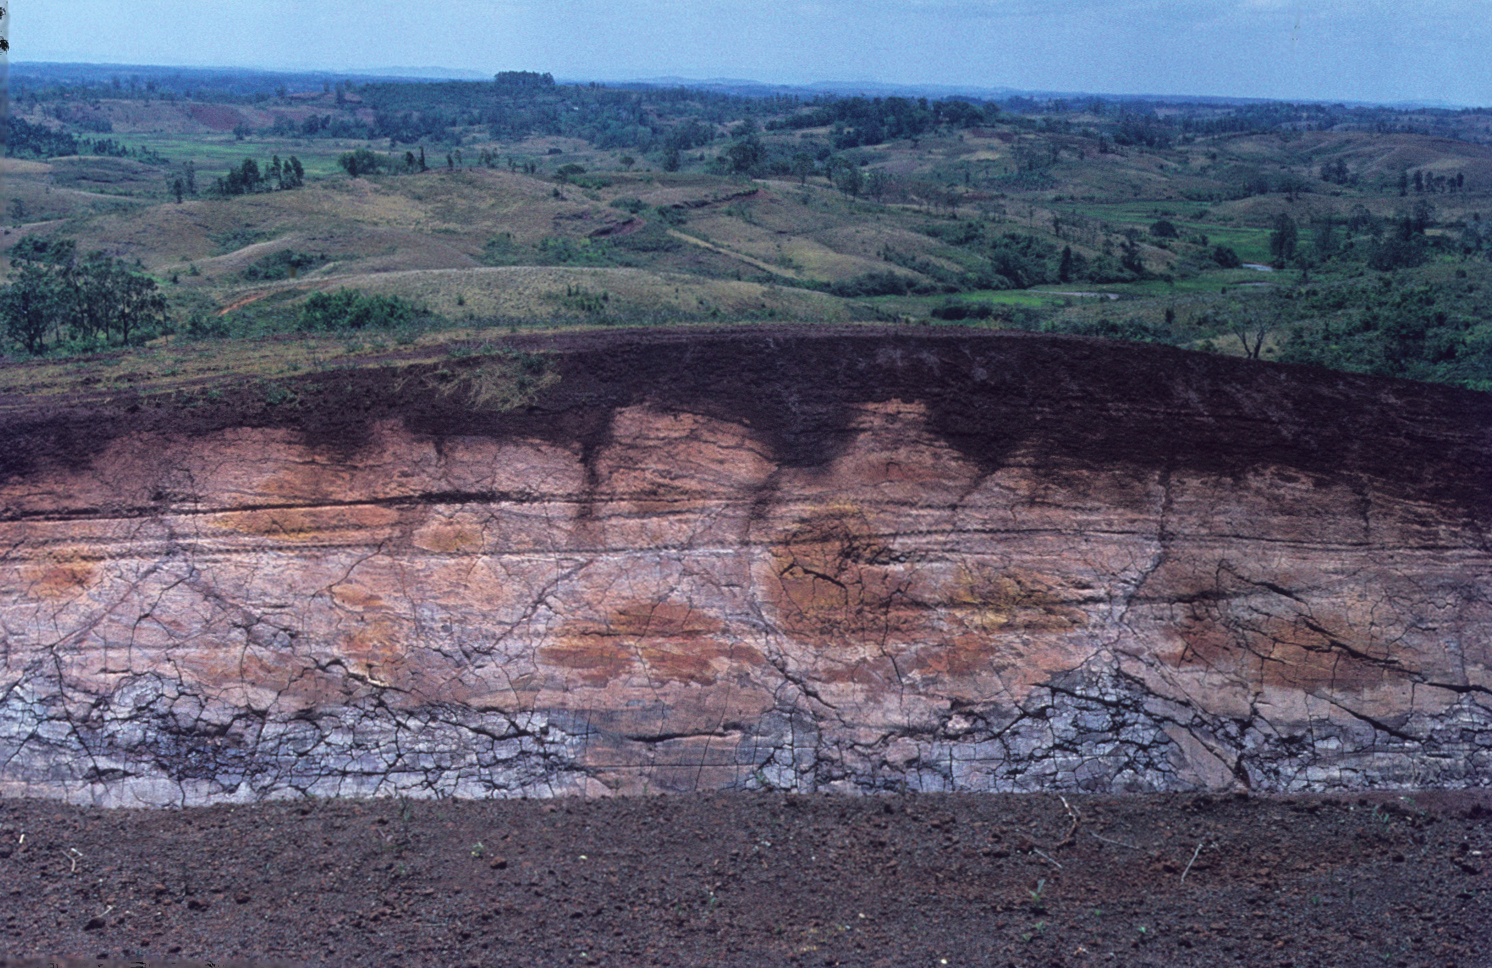
\includegraphics[width=1\linewidth]{obrazky/zvetravani/laterit}
	\caption{Zvětrávání bazaltového tufu (bílá barva) do saprolitu (žluto-bílá) a lateritu (tmavě hnědá), Vangaindrano, Madagascar (Zdroj: Werner Schellmann, CC BY-SA 2.5, via Wikimedia Commons)}
	\label{fig:laterit}
\end{figure}


\emph{Kaolinizace} je typický proces ekvatoriální humnidní zóny. Jedná se o dlouhodobé zvětrávání ve slabě kyselém prostředí. Důležité je velké množství srážek a možnost odtoku vody. Dochází k silném rozkladu původní strktury minerálů (živec, slída...). V místě zůstávají stabilnější prvky (\ce{Si} a \ce{Al}). Produktem jsou kaolinické zvětraliny (kaolinit).
%
%\subsubsection{Karbonatizace}
%Reakce minerálů s \ce{CO2} rozpuštěným ve vodě
%Vzniká aniont \ce{HCO3-} (nejčastější aniont v povrchových vodách)
%Dominantní zvětrávací proces u karbonátů (zvratná reakce)
%
%\subsubsection{Lateritizace}
%Proces vázaný na monzunové vnější tropy s vyhraněným obdobím sucha a vlhka
%Ve vlhkém období dochází k intenzivnímu rozpouštění a relativnímu hromadění 
%V období sucha dochází k výparu a \ce{Fe} a \ce{Al} se hromadí při povrchu jako sesquioxidy – tvoří pevné kůry při povrchu – laterity (bauxity)
%
%\subsubsection{Kaolinizace}
%Proces typický pro ekvatoriální humidní zónu
%Podmínky: 
%Dlouhodobé zvětrávání ve slabě kyselých podmínkách (nejmenší rozpustnost kaolinitu)
%Intenzivní srážky a možnost odtoku vody
%Silný rozklad původní struktury minerálů (živec, slída - alumosilikáty) - zůstávají stabilnější prvky - 
%Produkty – kaolinické zvětraliny (kaolinit)




%\subsubsection{Oxidace}
%Zvětrávání minerálů, které obsahují \ce{Fe} (pyrit, siderit atd.), ale také \ce{Al}, \ce{Mg}, \ce{Mn}, \ce{Cr}. (u těchto hornin je dominantní)
%Oxidovaná sloučenina ztrácí jeden elektron, 
%Reakcí sloučeniny s ve vodě rozpuštěným O2 dochází ke zvětšení objemu sloučeniny
%Vznikají oxidy a hydroxidy železa (většinou nerozpustné) – červená nebo žlutá barva (goethit, limonit, hematit)
%Exponované jsou horniny, které obsahují minerály s příměsí železa (pyroxeny, amfibolit, biotit) – červené povlaky na obnažených stěnách
%Příklad: 
%
%\subsubsection{Redukce}
%Opak oxidace – snížení oxidačního čísla 
%(\ce{Fe^3+} na  \ce{Fe^2+})
%Dochází k ní v prostředí s nedostatkem volného kyslíku
%Průběh v zamokřených zónách (např. močály atd)
%Výsledkem jsou látky chudé na kyslík – pyrit, markazit a jiné sloučeniny šedého, šedozeleného a modrého zbarvení

%\subsubsection{Hydratace a dehydratace}
%Včlenění vody do struktury sloučeniny
%Sloučenina, která přijímá vodu, zvětší svůj objem a tím může mechanicky působit na své okolí
%
%Příklad: Anhydrit x Sádrovec
%
%\ce{CaSO4 <--> CaSO4.2H20}
%

%\begin{myboxgreenwide}{Příklady rovnic chemického zvětrávání}[h]
%\textbf{Rozpouštění}: \\
%\ce{SiO2 + 2H2O -> Si(OH)4}\\
%
%\textbf{Hydrolýza:} \\
%\ce{$\underset{\text{ortoklas}}{\ce{2KAlSi3O8}} + 
%	\underset{\text{kys. uhličitá}}{\ce{2H2CO3}} + 
%	\underset{\text{voda}}{\ce{9H20}}$ -> \\
%	->
%	$\underset{\text{kaolinit}}{\ce{Al2Si2O3(OH)4}} + 
%	\underset{\text{kys. křemičitá}}{\ce{4H4SiO4}}  + 
%	\underset{\text{kationt draslíku}}{\ce{2K+}}  +
%	\underset{\substack{\text{hydrogenuhličitanový aniont}}}{\ce{2HCO-3}} $}
%
%\textbf{Oxidace:}\\
%\ce{4Fe^2+ + 3O2	->	2Fe2O3}
%
%\textbf{Hydratace a dehydratace} \\ Anhydrit x Sádrovec
%\ce{CaSO4 + 2H2O <--> CaSO4.2H20}
%
%\textbf{Karbonatizace} \\ Rozpouštění kalcitu
%\ce{CaCO3 + H2CO3 <-> Ca2+ + 2(HCO3^-)}\\
%\end{myboxgreenwide}


\section{Biologické zvětrávání}
Zvětrávání v důsledku činnosti organismů může mít charakter fyzikálního, ale i chemické zvětrávání. Pod fyzikálním biologickým zvětráváním si snadno můžeme představit růst kořenů rostlin, a jejich rozrušování hornin (rozšiřování puklin mezivrstevních spár apod.). Chemické zvětrávání je pak způsobené např.  Chemické zvětrávání organismy spíše urychlují (např. zvýšené množství \ce{CO2} v důsledku dýchání). 

\section{Zvětralinová pokrývka}
Produktem zvětrávání je zvětralinová pokrývka. Její podoba je odvislá na typu zvětrávání. Fyzikální zvětrávání produkuje hrubší, ostrohranný materiál a naopak produkty chemického zvětrávání jsou daleko jemnější a mají hlinitojílovitý charakter. Mocnost zvětralinové pokrývky souvisí s charakterem podnebí, délce zvětrávání a samozřejmě s odolností horniny. Na svazích je mocnost zvětraliny menší než na rovinách. Zvětralinu, která je na místě svého vzniku (\textit{in situ}) označujeme jako \emph{saprolit}, naopak zvětralina, která je gravitašně přesouvána z vyšších částí svahu se nazývá \emph{regolit}.

%\subsection{Zvětrávání a klima}
%\emph{Vlhké tropy a subtropy} jsou příznivé pro intenzivní chemické zvětrávání. Mocnost zvětraliny může dosahovat i stovek metrů. Díky vysoké organické aktivitě je voda v půdě značně kyselá (obohacena o \ce{CO2} a organické kysleiny), což způsobouje rozpouštění a vymývání \ce{Na+, Ca^2+, Cl+, Mg^2+} a dalších rozpustných složek. Naopak se tam hromadí nepohyblivé prvky \ce{Fe^3+, Al^3+}.
%
%\emph{Semiaridní a aridní oblasti}
%
%\emph{Mírné pásmo}
%
%\emph{Subpolární pásmo a vysokohorské prostředí}
%
%%\subsection{Produkty chemického zvětrávání}
%%Zvětralinový plášť, zvětrávací kůry
%%
%%\subsubsection{Typy zvětralinových kůr}
%%Zpevněné polohy ve zvětralinách, které se vyskytují na zemském povrchu nebo těsně pod ním
%%Vznikají aktivním nebo pasivním hromaděním některých prvků a sloučenin 
%%Pasivní akumulace (u málo mobilních prvků)
%%Ferricrete (hromadění Fe)
%%Alcrete (hromadění Al)
%%Aktivní akumulace (v případě mobilních prvků)
%%Silcrete (nad95 \% \ce{SiO2})
%%Calcrete (nad 80 \% \ce{CaCO3})
%%Gypscrete (nad 95 \% \ce{CaSO4.2H2O})



	\chapter{Svahy a svahové procesy}
	\section{Svahy}\index{svah}
Svah -- ukloněná část zemského povrchu je nejrozšířenějším a také nejdynamičtějším prvkem reliéfu krajiny. Svahy zabírají přibližně $90 \%$ povrchu souše. Většina svahů (cca $60 \%$) má sklon do \SI{10}{\degree}. 

V základu můžeme rozlišovat dva typy svahů.  A to podle toho, zda jsou pokryté sedimenty či půdou (\textit{soil-mantled hillslopes}). Tyto svahy jsou charakteristické svým hladkým průběhem s jen občasnými výchozy podloží. Druhým typem jsou svahy tvořené jen skalním podložím, neboli strukturní svahy (\textit{bedrock hillslopes}). Takovéto svahy jsou typické rozeklaným povrchem.


\subsection{Části svahu}
Svah lze rozčlenit do několika částí (jednotek, segmentů). Nejjednodušší rozdělení je do tří jednotek (Obr. \ref{fig:segmenty_svahu}. V horní části je konvexní jednotka, kde se sklon svahu s narůstající vzdáleností zvětšuje. Následuje lineární svah (sklon se nemění). Spodní část svahu má konkávní tvar, což znamená, že se sklon zmenšuje. V některých případech prostřední část svahu chybí a má konvexně-konkávní průběh \parencite{whiteConvexConcaveLandslopesGeometrical1966}. Přechod mezi jednotlivými segmenty může být pozvolný ale i ostrý.

\begin{figure}[h]
	\centering
	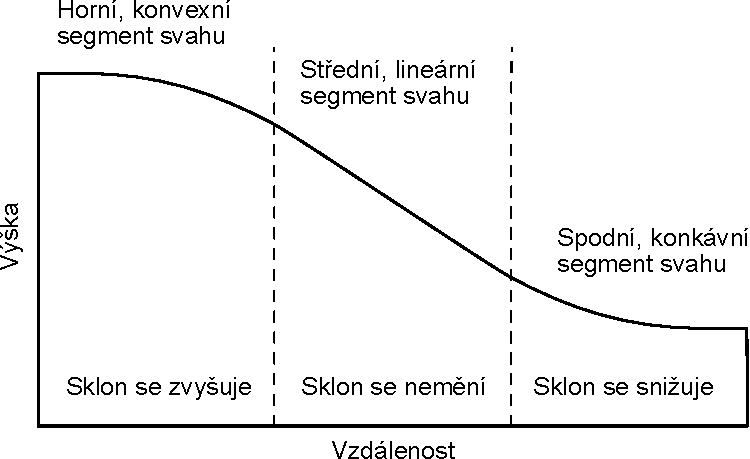
\includegraphics[width=1\linewidth]{obrazky/slope/segmenty_svahu}
	\caption{Tři základní segmenty svahu.}
	\label{fig:segmenty_svahu}
\end{figure}


Pojmenováním jednotlivých částí svahu se zabývala celá řada autorů. \textcite{dalrympleHypotheticalNineUnit1968} rozdělili svah do osmi částí:
\begin{enumerate}
	\item rozvodní část svahu o sklonu \SIrange{0}{1}{\degree}
	\item konvexní infiltrační část svahu se sklonem \SIrange{2}{4}{\degree}
	\item konvexní část svahu s plíživým pohybem materiálu 
	\item srub se sklonem minimálně \SI{45}{\degree}, zpravidla ale se sklonem přes \SI{65}{\degree}
	\item konkávní erozně-denudační část se sklonem \SIrange{26}{35}{\degree} kde probíhá transport materiálu
	\item konkávní akumulační část svahu
	\item fluviální část svahu v dosahu říční činnosti
	\item samotné říční koryto
\end{enumerate}

\subsection{Síly působící na svah}
Každá část svahu je pod vlivem gravitace. Ta vyvolává tíhové napětí. Pro zjednodušení si představte objekt který je na nakloněné rovině -- svahu. Tento objekt svou tíhou působí svisle na svah a vyvolává tíhové napětí. To můžeme rozložit do dvou složek. \emph{Normálová} složka resp. \emph{normálové napětí} působí kolmo na rovinu svahu. Po svahu dolů působí \emph{smykové napětí}. Smykové a normálové napětí vypočítáme podle rovnic:

\begin{align}
\text{Smykové napětí: }	\tau = \rho_{s}gz\sin{\theta}\\
\text{Normálové napětí: }	\sigma = \rho_{s}gz\cos{\theta}
\end{align}

Velikost smykového a normálového napětí je závislá na velikosti sklonu ($\theta$) svahu. S rostoucím sklonem narůstá smykové napětí a normálové klesá a naopak. Na horizontálním povrchu je smykové nulové, normálové napětí se rovná tíhovému. U kolmé stěny je naopak nulové normálové napětí a smykové se rovná tíhovému napětí.

\begin{figure}[h]
	\centering
	\includegraphics[width=1\linewidth]{obrazky/slope/svah_napeti}
	\caption{A: Rozklad tíhového napětí (síly) na normálové napětí ($\sigma$) a smykové napětí ($\tau$) v závislosti na sklonu svahu ($\beta$). B: ukázka rozložení sil na svahu (upraveno podle \textcite{selbyHillslopeMaterialsProcesses1993})}
	\label{fig:svahnapeti}
\end{figure}

\subsection{Koncept stability svahu}
Koncept stability svahu souvisí s působením výše uvedených sil (napětí) ve svahu. Ve své podstatě se jedná o poměr mezi silami, které drží materiál svahu v původní poloze a silami, které se snaží jej uvést do pohybu. Stabilita svahu tedy lze vyjádřit rovnicí:

\begin{equation}
\text{stabilita svahu} = \frac{\text{síly držící svah}}{\text{mobilizační síly}}	
\end{equation}

Poměr těchto sil se označuje jako faktor bezpečnosti (\textit{factor of safety}, FS) a ten vypočítáme jako podíl pevnosti ve smyku ($S$) a smykového napětí ($\tau$):

\begin{equation}
	\text{FS} = \frac{s}{\tau}	
\end{equation}

Svah je stabilní pokud je faktor bezpečnosti větší než jedna. Zpravidla se vyčleňují tři \enquote{pásma stability}:

\begin{itemize}
	\item FS $>1,3$ jedná se o stabilní svah
	\item FS z intervalu $(1;1,3>$ se jedná o podmínečně stabilní svah
	\item FS $=<1$ se jedná se o nestabilní svah
\end{itemize}

Pevnost ve smyku (\textit{shear strength}, S) lze vypočítat podle Coulomb-Terzagiho rovnice následovně:

\begin{equation}
	S = c+\sigma^{\prime}\tan{\phi}
\end{equation}

\emph{Koheze materiálu} ($c$) nebo také soudržnost materiálu je veličina, která udává jak jednotlivé částice materiálu drží pospolu. Je nezávislá na vnějších tlacích a je dána zejména chemickými vazbami a adhezí.

\emph{Úhel vnitřního tření materiálu} je závislý na velikosti částic, jejich tvarem a rozmítění.

\emph{Normálové napětí} zvyšuje úhel vnitřního tření. Jelikož proti normálovému napětí působí tlak vody v pórech (tzv. pórové tlaky) snižuje se o jejich hodnotu velikost normálového napětí. Hovoříme potom o \emph{efektivním normálovém napětí} ($\sigma^{\prime}$).

Stabilita svahu je stav, který se mění v čase v závislosti na celé řadě podmínek. Může se zvyšovat, ale i snižovat. 

Tabulka \ref{tab:stabilita_faktory} obsahuje příklady různých příčin sesuvů a jiných svahových pohybů. Tyto příčiny můžeme rozdělit do tří skupin:
\begin{enumerate}
	\item Predispozice
	\item Přípravné faktory
	\item Spouštěcí faktory
\end{enumerate}

\emph{Predispozice} jsou vlastnosti hornin, kterými je svah budován (např. koheze, pevnost materiálu), přítomnost a orientace tektonických struktur (pukliny), sklon, výška svahu a podobně. \emph{Přípravné faktory} způsobují postupné snižování stability svahu. Například zvětráváním horniny může docházet ke snižování koheze, rozpouštění tmele, který drží jednotlivé klasty. Akumulací sedimentů v horní části svahu dochází k zatěžování svahu (roste ve svahu smykové napětí). \emph{Spouštěcí faktory} jsou ty, které svah uvedou do pohybu. Způsobí tedy to, že se faktor bezpečnosti sníží na jedna a méně. Spouštěcím faktorem může být například zemětřesení, které ve svahu vyvolává přechodné napětí. Významným spouštěčem jsou intenzivní srážky, které způsobují zvýšení pórových tlaků (a tedy snížení normálového napětí).

\begin{figure}[h]
	\centering
	\includegraphics[width=1\linewidth]{obrazky/slope/stability_diagram}
	\caption{Faktory ovlivňující stabilitu svahu. V případě destabilizace svahu pak nastupují faktory, podporující nestabilitu svahu (upraveno podle \textcite{gladeLandslideGeomorphologyChanging2010})}
	\label{fig:stability_diagram}
\end{figure}

\begin{figure*}[h]
	\centering
	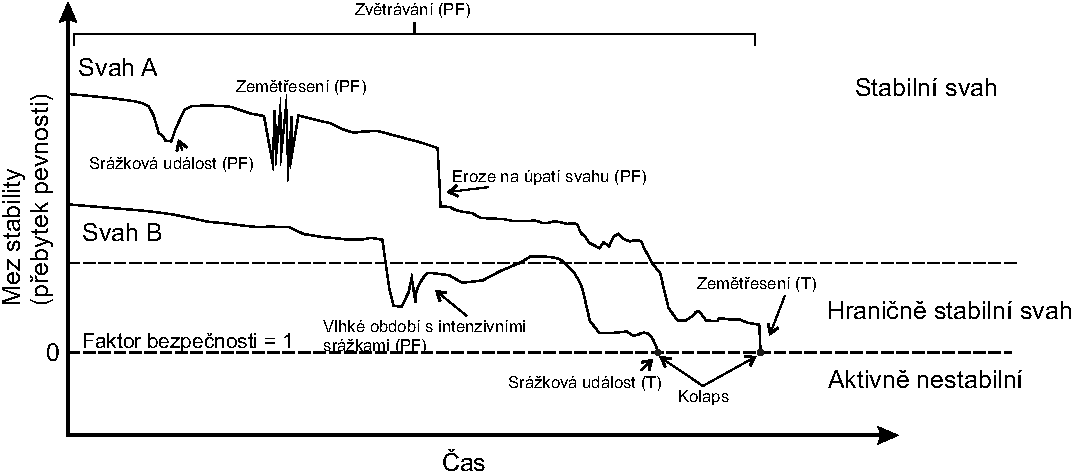
\includegraphics[width=1\linewidth]{obrazky/slope/time_stability}
	\caption{Vývoj stability dvou hypotetických svahů. Přípravné faktory (PF) postupně nebo nárazově snižují stabilitu svahu (snižují pevnost ve smyku). Spouštěcí faktory (triggery -- T) jsou ty, které sníží pevnost ve smyku tak, že faktor bezpečnosti $ \leq 1$ (upraveno podle \textcite{popescuSuggestedMethodReporting1994} a \textcite{mccollLandslideCausesTriggers2015})}
	\label{fig:timestability}
\end{figure*}

%\todo[inline]{Glade Crozier obrázek faktory}
%\todo[inline]{McColl svahy vývoj}
\begin{table*}
	\small
	\begin{tabularx}{\textwidth}{@{}XXXX@{}}
		\toprule
		\multicolumn{4}{@{} p{\textwidth} @{}}{\textbf{Predispozice}} \\
		\midrule
		\multicolumn{4}{@{} p{\textwidth} @{}}{Plastický, měkký materiál} \\
		\multicolumn{4}{@{} p{\textwidth} @{}}{Sypký materiál} \\
		\multicolumn{4}{@{} p{\textwidth} @{}}{Navětralý materiál} \\
		\multicolumn{4}{@{} p{\textwidth} @{}}{Tektonicky porušený materiál} \\
		\multicolumn{4}{@{} p{\textwidth} @{}}{Příhodně orientované diskontinuity (např. vrstevní plochy, pukliny, zlomy)}\\
		\multicolumn{4}{@{} p{\textwidth} @{}}{Kontrast mezi propustností hornin} \\
		\multicolumn{4}{@{} p{\textwidth} @{}}{Kontrastní pevnost hornin (pevné horniny v nadloží plastických např. pískovce na jílovcích)}\\ 
		\midrule \midrule
		& & \textbf{Proces} & \\ 
		\midrule
		\textbf{\textbf{Přípravné faktory}} & \textbf{Geomorfologický} & \textbf{Fyzikální} & \textbf{Antropogenní} \\ 
		\midrule
		Nárůst výšky svahu nebo sklonu  & Tektonické pochody, vulkanismus, výzdvih po odlednění &  & Výkopy ve svahu, násypy \\
		& Fluviální, marinní nebo ledovcová eroze &  &  \\
		Ztráta opory & Ústup ledovce &  & Odtěžení paty svahu \\
		Odkrytí potenciálních smykových ploch & Eroze &  & Výkopy ve svahu \\
		Snížení pevnosti horniny & Sufoze, rozpouštění & Zvětrávání & Hloubení tunelů, dolů; odlesnění\\ 
		& Zvětrávání & Únava materiálu &  \\
		Zatěžování svahu & Postupná akumulace sedimentů  &  &Stavba, ukládání materiálu -- výsypky  \\
		Dlouhodobé zvyšování hladiny podzemní vody & Klimatické změny &  & Infiltrace srážkových vod, prasklé potrubí  \\
		&  &  & Zavlažování \\
		&  &  & Odstranění vegetace \\ 
		\midrule \midrule
		\textbf{Spouštěče} & \textbf{Geomorfologické} & \textbf{Fyzikální} & \textbf{Antropogenní} \\ 
		\midrule
		Rychlý nárůst pórových tlaků  & Rychlé zatížení sedimenty z Undrained loading from rapid emplacement of sediment & Srážky & Zatížení rychlým uložením navážky  \\
		&  &  Tání sněhu/ledu &  \\
		Rychlý pokles hladiny podzemní vody & Protržení přírodních hrází &  & Snižování hladiny v nádržích \\
		Přechodná napětí&  & Zemětřesení& Vibrace strojů \\
		&  & Vítr &  \\
		Snížení pevnosti&  & Degradace permafrostu &  \\
		&  & Zvětrávání &  \\
		&  & Únava materiálu &  \\
		Zatěžování svahu & Jiné sesuvy & Srážky & Stavby \\
		\bottomrule
	\end{tabularx}
		\caption{Příklady příčin sesuvů \parencite[podle][]{mccollLandslideCausesTriggers2015}}
		\label{tab:stabilita_faktory}
	
\end{table*}

\section{Gravitační svahové pochody}

\subsection{Světová klasifikace svahových pohybů}
Gravitační svahové pohyby jsou způsobeny přímým působením gravitace. Dalo by se říct, že \enquote{klasickou} a celosvětově zaužívanou klasifikací svahových pohybů je klasifikace \textcite{crudenLandslideTypesProcesses1996} s poslední úpravou od Hungra \parencite*{hungrVarnesClassificationLandslide2014}. Tato klasifikace je založena na třech kritériích:
\begin{itemize}
	\item rychlost pohybu
	\item mechanismus pohybu
	\item typ horniny (skalní hornina/zemina)
\end{itemize}

Svahové pohyby rozdělují do následujících šesti skupin:
\begin{itemize}
	\item Řícení (\textit{fall})
	\item Odklánění (\textit{topple})
	\item Sesouvání (\textit{slide})
	\item Boční rozšiřování (\textit{spread})
	\item Tečení (\textit{flow})
	\item Svahové deformace (\textit{slope deformation})
\end{itemize}

\begin{figure*}
	\centering
	\includegraphics[width=1\linewidth]{obrazky/slope/landslide_type}
	\caption{Typy gravitačních svahových pohybů (Upraveno podle USGS)}
	\label{fig:landslidetype}
\end{figure*}


%\begin{table*}[]
%	\begin{tabular}{@{}lll@{}}
%		\toprule
%		Typ pohybu & Skalní horniny                       & Zeminy                            \\ \midrule
%		Řícení             & 1. Rock/ice fall           & 2. Boulder/debris/silt falla    \\ \midrule
%		\multirow{2}{*}{Odsedání/toppling}            & 3. Blokové odsedání          & 5. Odesdání štěrku/písku/siltu        \\ 
%		& 4. Flexurní odsedání    &                                 \\ \midrule
%		\multirow{5}{*}{Sesouvání}             & 6. Skalní rotační sesuv       & 11. Clay/silt rotational slide     \\
%		& 7. Rock planar slidea      & 12. Clay/silt planar slide      \\
%		& 8. Rock wedge slidea       & 13. Gravel/sand/debris slidea   \\ \midrule
%		& 9. Rock compound slide     & 14. Clay/silt compound slide    \\
%		& 10. Rock irregular slidea  &                                 \\ \midrule
%		\multirow{2}{*}{Spread}            & 15. Rock slope spread          & 16. Sand/silt liquefaction spreada \\
%		& 17. Sensitive clay spreada &                                 \\ \midrule
%		\multirow{9}{*}{Flow}              & 18. Rock/ice avalanchea        & 19. Sand/silt/debris dry flow      \\
%		&                            & 20. Sand/silt/debris flowslidea \\
%		&                            & 21. Sensitive clay flowslidea   \\
%		&                            & 22. Debris flowa                \\
%		&                            & 23. Mud flowa                   \\
%		&                            & 24. Debris flood                \\
%		&                            & 25. Debris avalanchea           \\
%		&                            & 26. Earthflow                   \\
%		&                            & 27. Peat flow                   \\ \midrule
%		\multirow{3}{*}{Slope deformation} & 28. Mountain slope deformation & 30. Soil slope deformation         \\
%		& 29. Rock slope deformation & 31. Soil creep                  \\
%		&                            & 32. Solifluction                \\ 
%		\bottomrule
%	\end{tabular}
%	\caption{HUngr varnes klasifikace}
%	\label{tab:sesuvy_Hungr}
%\end{table*}

\subsubsection{Řícení}
\emph{Řícení} (\textit{fall}) je nejrychlejším gravitačním procesem, kdy rychlost pohybu činí řádově \si{\metre\per\second}. K řícení dochází na strmých svazích ($>\SI{45}{\degree}$). Pohyb hmoty je alespoň v části trajektorie realizován volným pádem a následně se horninové fragmenty kutálejí či poskakují. Řícení můžeme rozlišit podle materiálu, který se účastní pohybu na: skalní řícení, suťové řícení a řícení v zeminách (spraši).

Řícení může nabývat celé řady podob. \emph{Sesypávání} probíhá nejčastěji v zeminách. Dále může docházet k \emph{odpadávání úlomků} ze skalních výchozů. Na úpatí skalní stěny se tvoří osypy (\textit{talus}). \emph{Odvalové řícení} je způsobeno odkláněním bloku (viz níže), kdy po překročení kritické meze dojde k jeho kolapsu. \emph{Planární řícení} zahrnuje podobně jako odvalové řícení větší masu horniny. V iniciální fázi dochází k sesouvání horniny podél planární smykové plochy a až následně dojde k pohybu volným pádem a tedy řícení. Jedná se často o velké katastrofické události.

\subsubsection{Odklánění}
\emph{Odklánění} nebo také \emph{odsedání} (\textit{toppling}) je proces, kdy dochází k pohybu horninového bloku kolem horizontální osy. V podstatě jde překlápění bloku ze svahu dolů. Jedná se o pomalé pohyby (\si{\milli\metre\per\rok}). Avšak ve finální fázi může dojít až ke katastrofickému zrychlení pohybu -- zřícení (\si{\metre\per\second}).

\textcite{goodmanTopplingRockSlopes1976} rozlišují dva základní druhy odklánění. Prvním typem je blokové odklánění. Jedná se o uklánění velkých bloků hornin. Predispozicí jsou strmě do svahu zapadající diskontinuity, které od sebe oddělují jednotlivé horninové bloky a případně doplněné o mírně ukloněné diskontinuity tvořící bázi bloků. Druhý typ je ohybové odklánění (\textit{flexural toppling}). K této deformaci může docházet na strmých svazích, které jsou budované horninami se strmě zapadajícími diskontinuitami s velmi malým rozestupem. K odklánění může docházet i v zeminách např. na březích vodních toků.

\subsubsection{Sesouvání}
\emph{Sesouvání} (\textit{slide}) je relativně rychlý, klouzavý pohyb horninové hmoty na svahu podél jedné nebo více \emph{smykových ploch}. Rychlost je variabilní, může se pohybovat v řádu \si{\milli\metre\per\rok}--\si{\metre\per\second}. Rychlost pohybu uvolněné hmoty se směrem do hloubky nemění.

\emph{Sesouvání je proces}, jehož výsledný tvar je \emph{sesuv}.

Sesuv má tři základní části: 
\begin{itemize}
	\item Odlučná oblast (výchoz smykové plochy)
	\item Transportní zóna
	\item Akumulační zóna
\end{itemize}

Smyková plocha je plocha, podél které došlo k sesouvání. Sesouvání může probíhat i po více smykových plochách. Podle tvaru smykové plochy můžeme sesuvy rozlišit na dva základní typy: rotační a translační sesuvy.

\emph{Rotační sesuv} (\textit{rotational slide} nebo \textit{slump}, obr. \ref{fig:rotacni}) má smykovou plochu zakřivenou, válcovou. Na tvar smykové plochy nemají vliv geologické struktury (pukliny, vrstevní plochy). Z důvodu zakřivení smykové plochy dochází k naklonění povrchu sesunutých bloků proti svahu. Rotační sesuvy jsou typické pro homogenní materiály, kohezivní zeminy a měkké horniny, které mají v nadloží často vrstvu pevných hornin. Jelikož je pohyb podél zakřivené smykové plochy samostabilizační, jsou rotační sesuvy zpravidla pomalejší.

\begin{figure}[h]
	\centering
	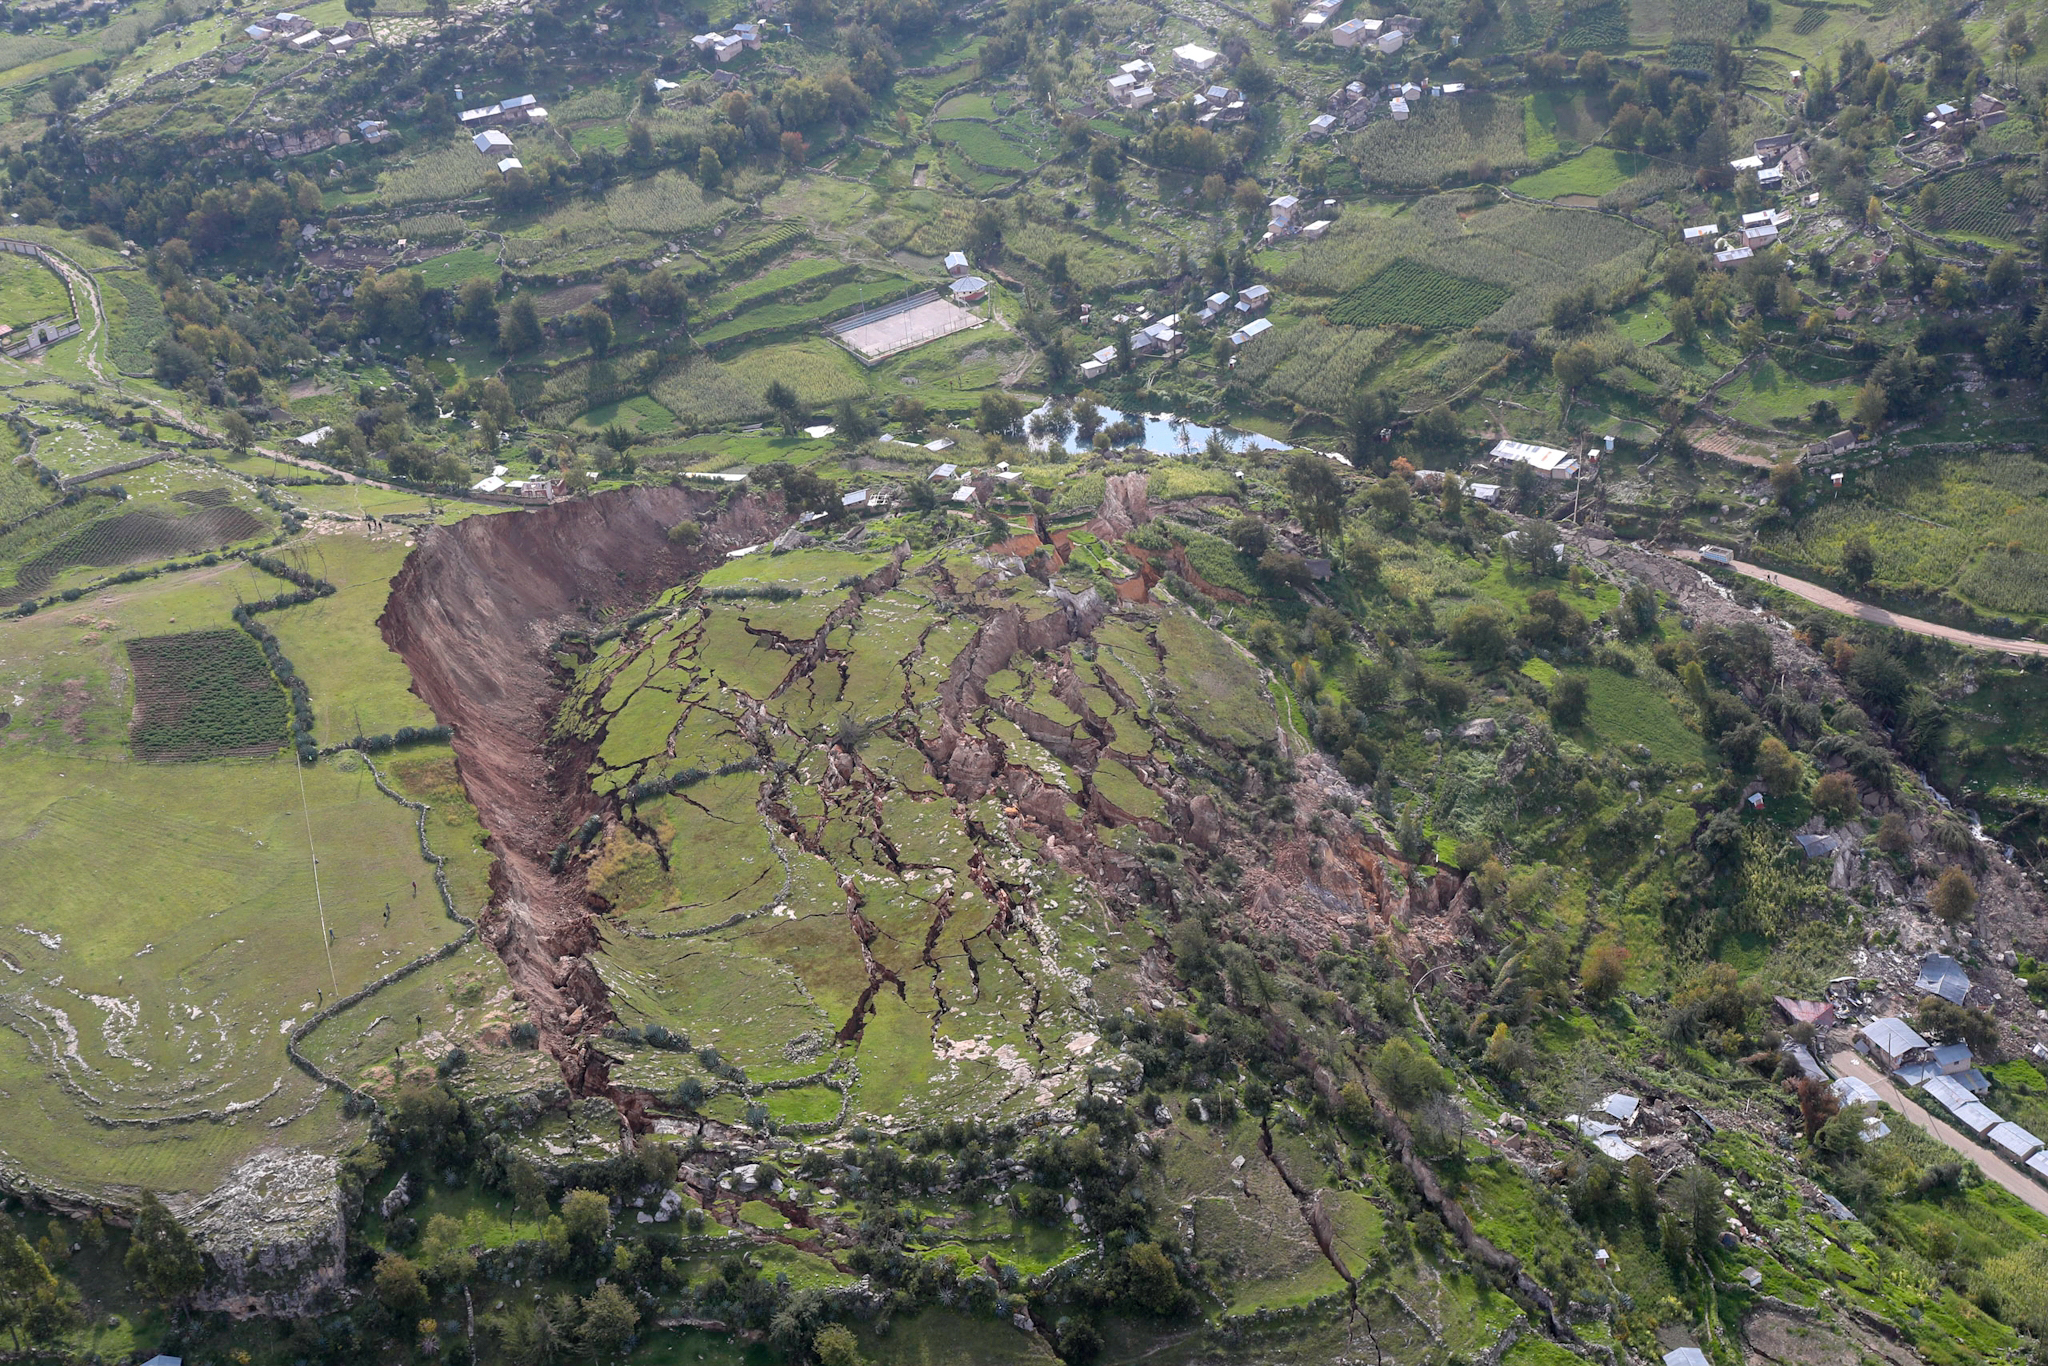
\includegraphics[width=1\linewidth]{obrazky/slope/rotacni}
	\caption{Rotační sesuv poblíž Cusca, Peru  roku 2018 (autor: Ministerio de Defensa del Perú - \url{https://www.flickr.com/photos/ministeriodedefensaperu/39935939755/in/dateposted/}, CC BY 2.0}
	\label{fig:rotacni}
\end{figure}


\emph{Translační} nebo také \emph{planární sesuvy} mají smykovou plochu rovnou. Ta je většinou predisponovaná nějakou nespojitostí v hornině. Může se jednat například o vrstevní plochy, pukliny, plochy foliace apod. Translační sesuvy ale mohou vznikat i na rozhraní sediment -- skalní podloží. Pokud se horninová masa pohybuje jako jeden celek po jedné smykové ploše, označujeme to jako \emph{blokový sesuv}. Specifickým typem translačních sesuvů jsou tzv. \textit{wedge slides} -- klínové sesuvy. Smyková plocha je tvořená zpravidla dvěma strukturami (např. puklinami), které oddělují nestabilní blok od zbytku skalního masivu. Na rozdíl od rotačních sesuvů nejsou translační sesuvy samostabilizační, tudíž se jedná zpravidla o velice rychlé události. Mělké planární sesuvy (vzniklé ve zvětralinách) vznikají často po intenzívních deštích. 

Některé sesuvy mohou mít složenou smykovou plochu. Běžný typ \emph{sesuvu podél složené smykové plochy} má v horní části zakřivenou smykovou plochu přecházející pak v planární níže po svahu.
\begin{figure*}
	\centering
	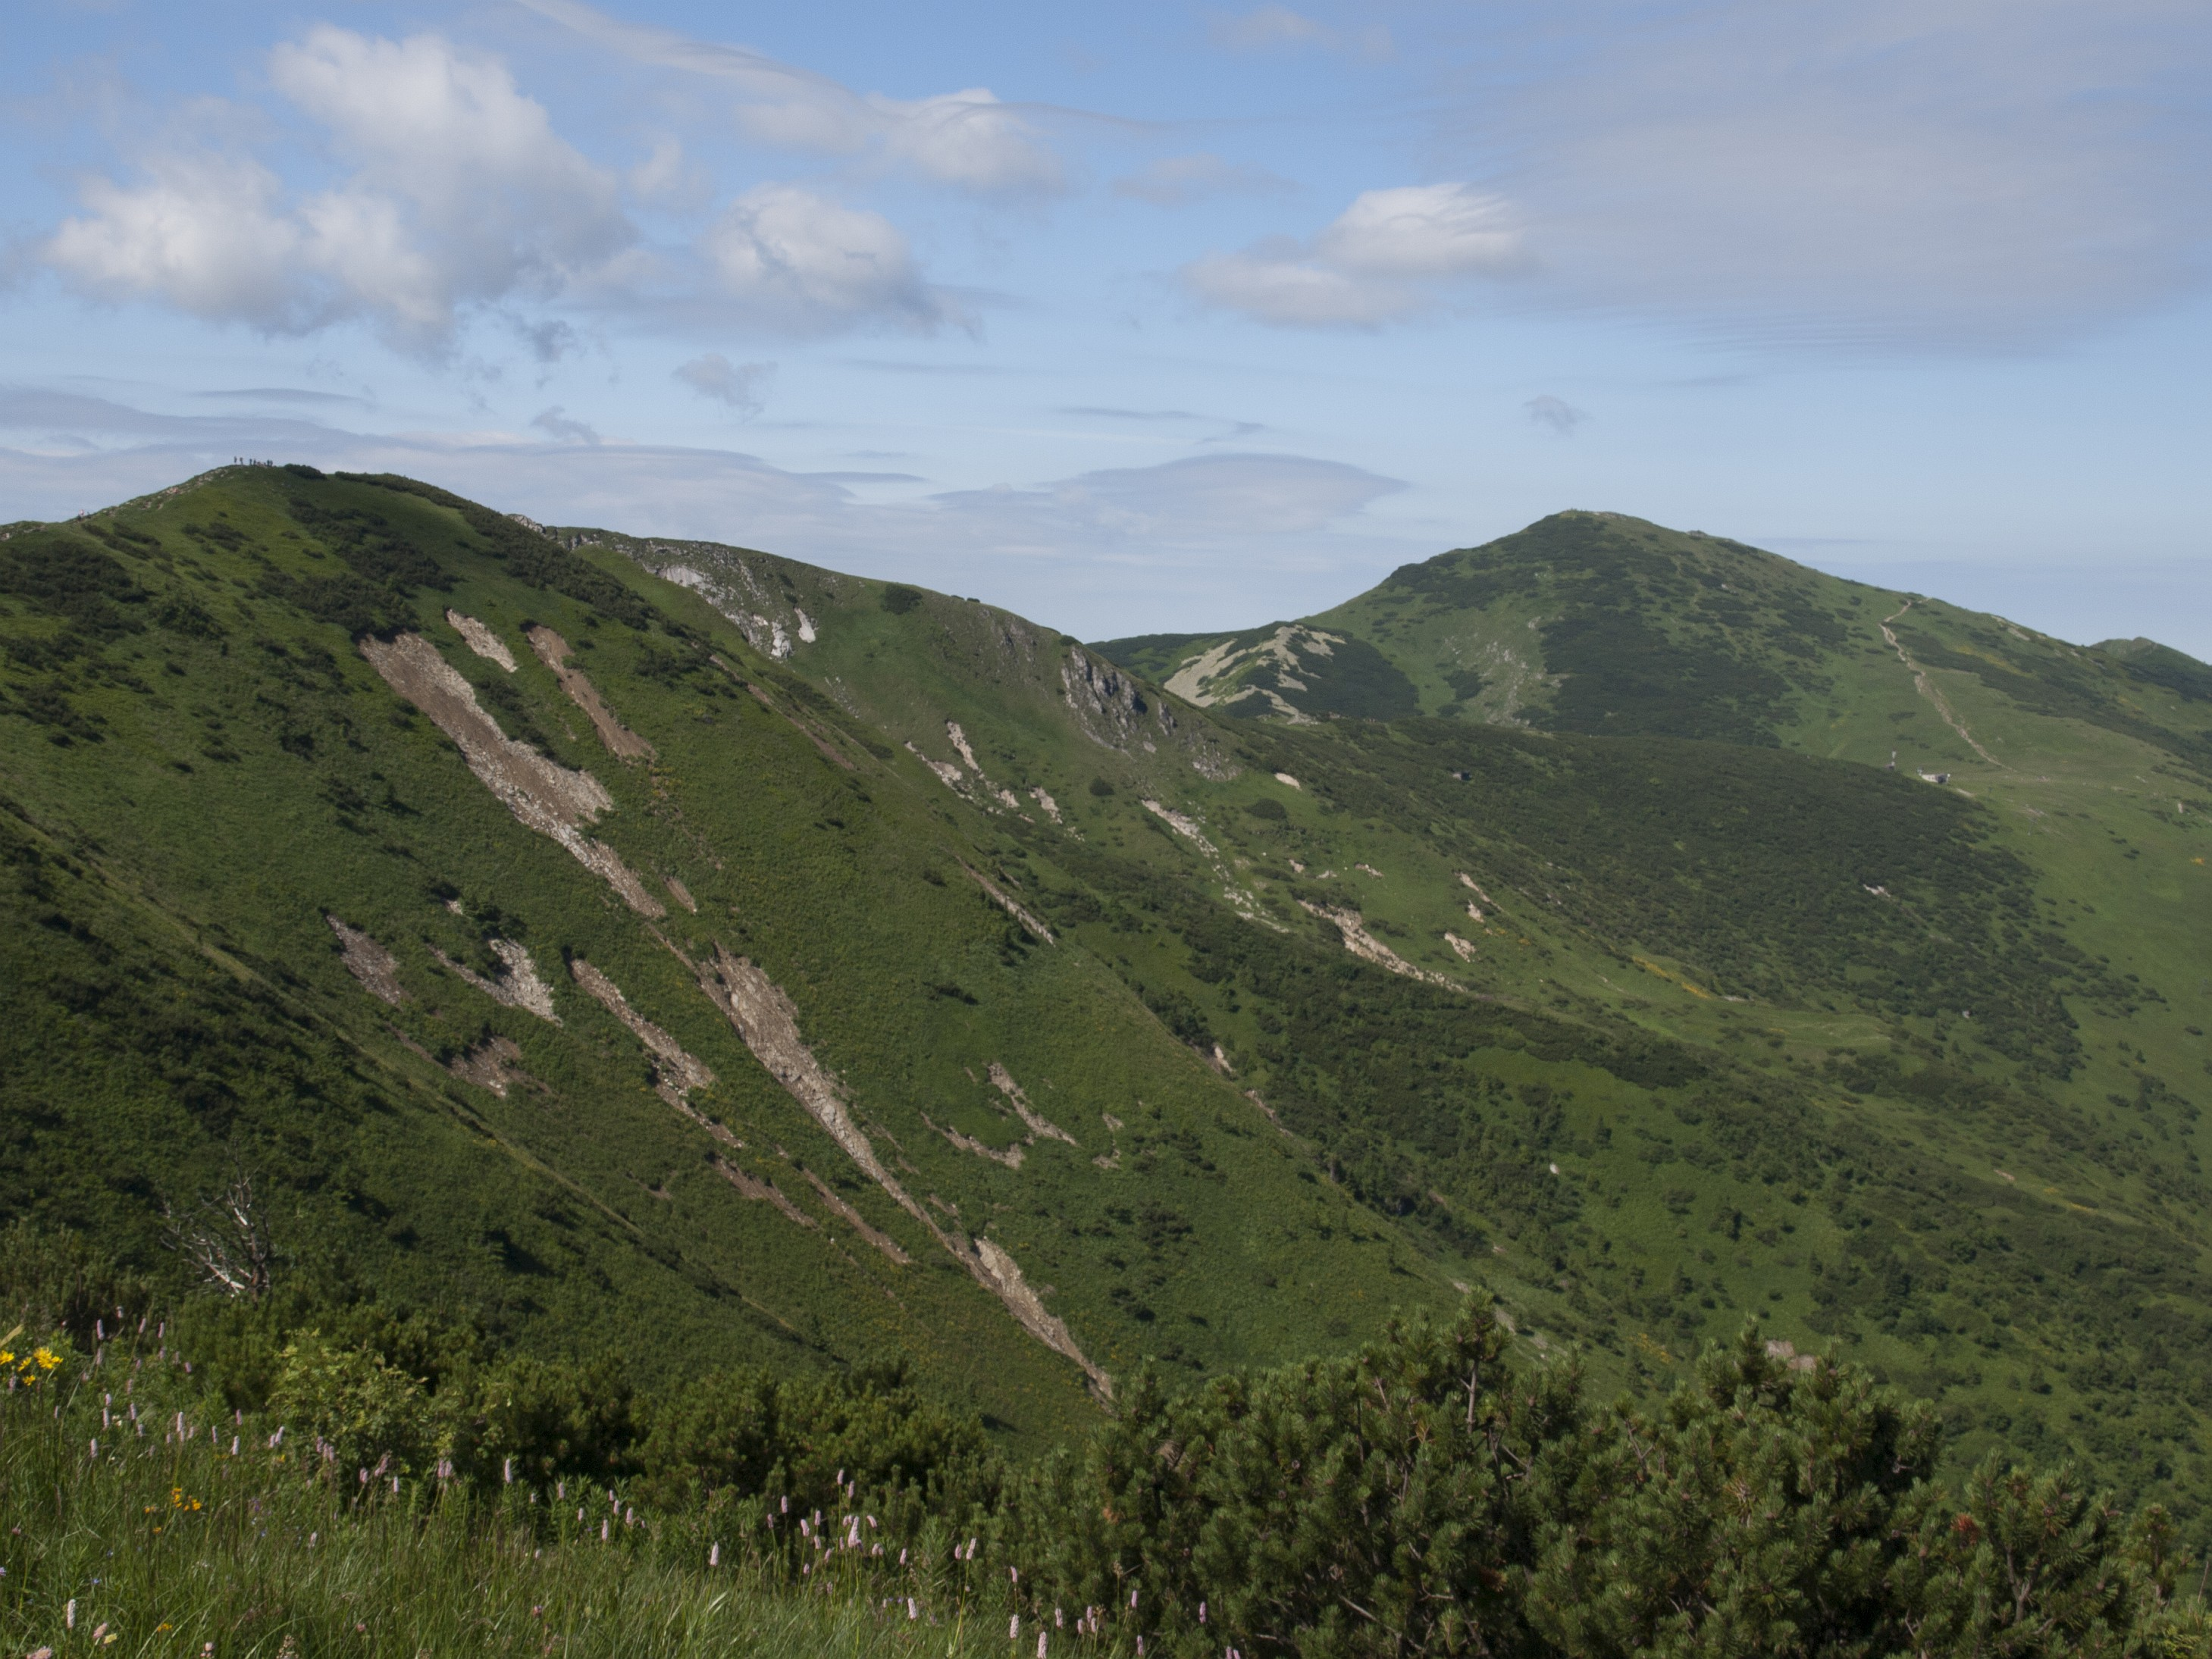
\includegraphics[width=1\linewidth]{obrazky/slope/melke}
	\caption{Mělké translační sesuvy ve zvětralině vzniklé na svazích Chlebu a Hromové v roce 2014 v důsledku intenzivních srážek. Při události došlo k jejich následné transformaci do blokovobahenního proudu, který způsobil velké škody ve Vrátné dolině (Malá Fatra, Slovensko).}
	\label{fig:melke}
\end{figure*}

\subsubsection{Boční rozšiřování}
\emph{Boční rozšiřování} (\textit{lateral spreading}) je rozevírání trhlin pouze horizontálním pohybem v důsledku extenze rigidních (pevných) hornin v nadloží měkkých a plastických hornin. Může se jednat například od pískovce v nadloží jílovců. K bočnímu rozvolňování dochází zpravidla v důsledku pomalé deformace plastického podloží. 

Jedná se o pomalé pohyby (\si{\milli\metre\per\rok}), které ale mohou být extrémně rychlé ve ztekucených zeminách.

\subsubsection{Tečení}
Tečení je svahový pohyb, kdy materiál je ve viskózním stavu. Rychlost tečení je různorodá. Pohybuje se od \si{\centi\metre\per\den} až $>\SI{100}{\kilo\metre\per\hour}$. Výsledný tvar je \emph{proud}. Blokovobahenní proud, mura (debris flow). Hlavní příčinou tečení je nasycení materiálu vodou. Tečením mohou být transportovány i bloky hornin i metrových velikostí. 

\label{blokovo}
Častým typem tečení jsou tzv. \emph{blokovobahenní proudy} (\textit{debris flow}), také nazývané \emph{mury}. Vyskytují se typicky v horském terénu. Jedná se o rychlý pohyb ztekuceného materiálu (bahna a velkých balvanů) ve stržích či údolích prvních řádů, kde se tyto proudy pravidelně opakují. K blokovobahenním proudům dochází zejména po prudkých deštích. Často se vyskytují během povodňových událostí. Prvopočátek blokovobahenního proudu může být v podobě sesuvu vodou saturovaného koluvia. Když tento sesuv narazí na dno strže/údolí dochází ke ztekucení materiálu a vzniku samotného blokovobahenního proudu. Ten má velkou erozní schopnost a díky tomu nabírá další hmotu během svého pohybu.  V případě, že tekoucí materiál neobsahuje velké balvany a skládá se především ze siltu hovoříme o \emph{bahnotoku}. Pro velké bahnotoky a blokovobahenní proudy ze sopečného materiálu se používá termín \emph{lahary}.

\begin{figure}
	\centering
	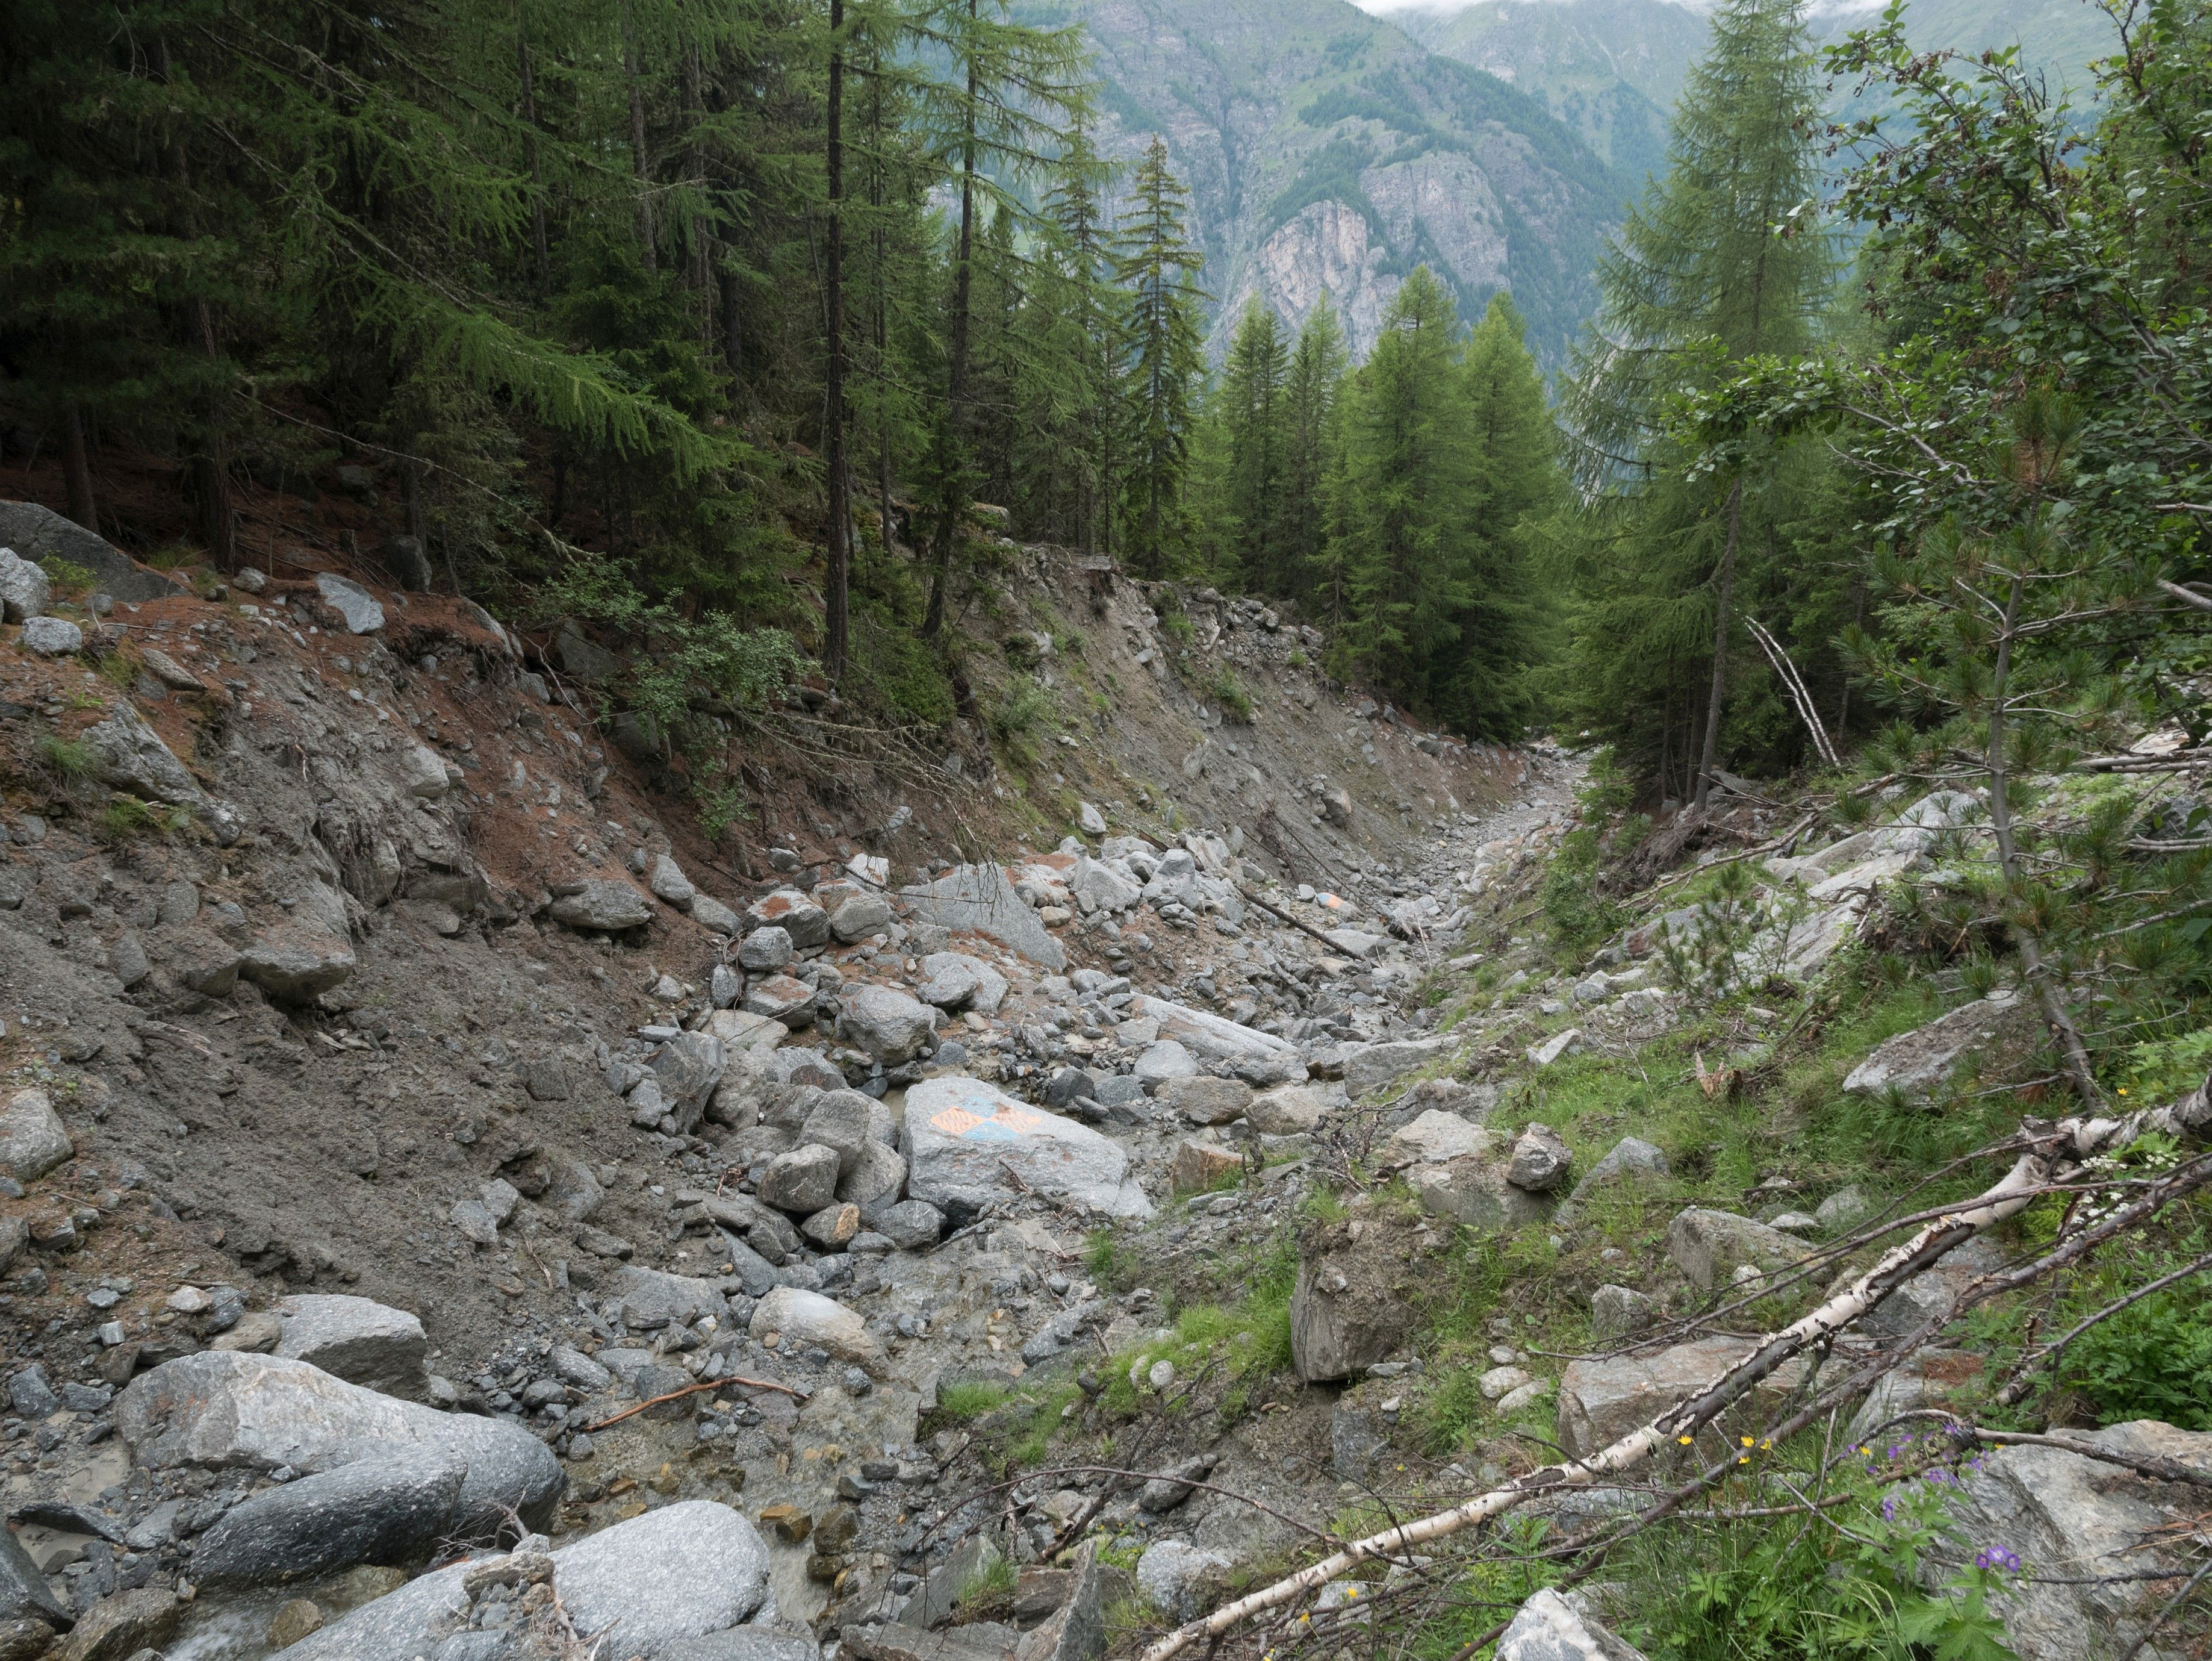
\includegraphics[width=1\linewidth]{obrazky/slope/debris_flow}
	\caption{Dráha blokovobahenních proudů, Švýcarsko.}
	\label{fig:debrisflow}
\end{figure}


\emph{Zemní proud} (\textit{earthflow}) je relativně pomalý proces tečení zemin. Pro zemní proudy jsou typická období klidu (desítky i stovky let) proložená epizodami náhlé aktivity. Jejich rychlost pohybu se pohybuje od metrů za rok až po metry za hodinu. Délka zemních proudů je v řádu desítek metrů až několika kilometrů.

\emph{Skalní laviny} jsou extrémním svahovým procesem. Jejich počátek je zpravidla v podobě velkého skalního sesuvu, který se ale záhy rozpadá a výsledkem je extrémně rychlý proud úlomků hornin. Objem sesunutých hornin bývá $> \SI{1}{\mega\metre\cubed}$ a může dosahovat i desítek \si{\giga\metre\cubed}.
Skalní laviny mají oproti klasickým sesuvům ohromnou mobilitu, tudíž mohou dosáhnout značných vzdáleností od svého počátku (i desítky \si{\kilo\metre}). Rychlost pohybu je v řádu stovek kilometrů za hodinu.

\subsubsection{Svahové deformace}
Termínem \emph{svahové deformace} označujeme extrémně pomalé pohyby (\si{\milli\metre} až \si{\metre\per\rok}) horninových hmot na svahu. Často jsou tyto pomalé pohyby jen přípravnou fází pro jiné, rychlejší svahové procesy. Pomalými pohyby není překročena mez pevnosti hornin, jedná se tak o plastické pohyby, při kterých nevznikají smykové plochy. Podle hloubky do které zasahují pohyby svahové deformace dělíme na:

\begin{itemize}
	\item Povrchové ploužení
	\item Deformace skalních (horských) svahů označované i jako hlubinné ploužení
\end{itemize}

\paragraph{Povrchové ploužení}
Povrchové ploužení je pomalý plastický pohyb zvětralinového pláště (deluvia) a půd na svazích. Projevuje se už na velmi mírných svazích. Hloubkový dosah je v řádu \si{\metre}. K ploužení dochází z důsledku cyklických objemových změn ve zvětralinách v důsledku klimatický vlivů. K expanzi dochází např. při zvlhčení nebo mrznutí, kontrakci pak při vysychání a tání. Dále se uplatňuje růst ledových krystalků \emph{jehlovitého ledu}. Mezi důsledky povrchového ploužení, ale i dobrým identifikačním znakem jsou ohnuté kmeny stromů (tzv. opilý les). Ploužení mů§že způsobovat také  \emph{hákování vrstev}, což je ohnutí vrstev směrem po svahu. 

\emph{Soliflukce} označuje pomalé stékání činné vrstvy permafrostu po zmrzlém podloží, což vede ke vzniku soliflukčních laloků.

\paragraph{Hlubinné ploužení}
Pro hlubinné ploužení se často používá termín \emph{sackung}. Tento proces postihuje velké objemy hornin do značné hloubky (desítky až stovky metrů). Rychlost hlubinného ploužení je velice nízká, což znamená, že se veškeré viditelné formy na svahu vyvíjejí velice pomalu. Sackung se typicky projevuje \emph{zdvojenými hřbety}, různými \emph{stupni na svazích} (Obr \ref{fig:sackung}). Spodní část svahu je často vyboulená. Tento proces vyboulení se označuje jako \emph{bulging}.

\begin{figure}[h]
	\centering
	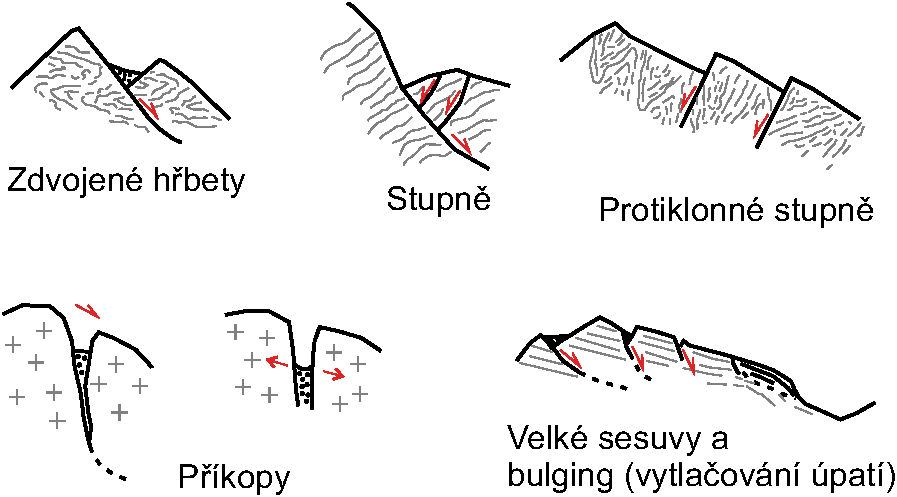
\includegraphics[width=1\linewidth]{obrazky/slope/sackung}
	\caption{Projevy hlubinného ploužení (sackungu) \parencite[podle][]{agliardiStructuralConstraintsDeepseated2001}}
	\label{fig:sackung}
\end{figure}

\subsection{Československá klasifikace svahových pohybů}
Na území ČR je používaná klasifikace svahových pohybů podle Nemčoka, Paška, Rybáře \parencite*{nemcokDeleniSvahovychPohybu1974}. Svahové pohyby dělí na základě mechanismu pohybu a rychlosti pohybu. Tato klasifikace je jednodušší na počet základních typů svahových pohybů, ale v podstatě pokrývá vše co je uvedené v mezinárodní Varnesově klasifikaci. Svahové pohyby dělí do čtyř základních skupin:
\begin{itemize}
	\item ploužení
	\item sesouvání 
	\item stékání
	\item řícení
\end{itemize}

Co je důležité, tak autoři rozlišují \emph{svahový pohyb}, tedy proces a \emph{svahovou deformaci}, což je výsledný tvar. 

\subsubsection{Ploužení}
Do ploužení spadají dlouhodobé pomalé (\si{\milli\metre\per\rok} až \si{\centi\metre\per\rok}). Hranice mezi pohybující se horninovou hmotou a pevným podložím je nezřetelná. V důsledku ploužení může docházet k tzv. hákování vrstev (Obr. \ref{fig:hakovani}). Jedná se ohnutí vrstev po svahu dolů. 
\begin{figure}[h]
	\centering
	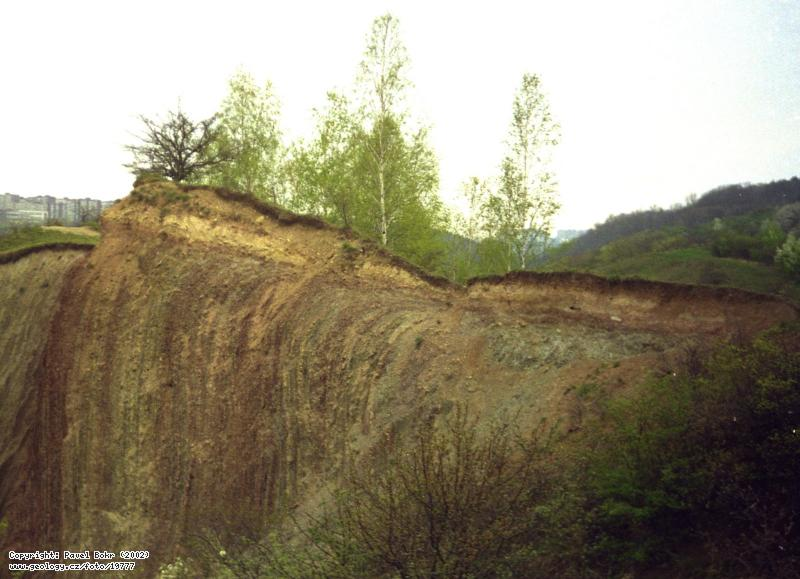
\includegraphics[width=1\linewidth]{obrazky/slope/hakovani}
	\caption{Ukázka hákování vrstev devonských vápenců v Praze-Hlubočepích (Zdroj: BOKR, P. (2002): Foto - Hákování vrstev v Praze - Hlubočepích. In: Fotoarchiv České geologické služby [online databáze]. Praha, Česká geologická služba [cit. 2022-02-15]. Dostupné z URL \url{http://www.geology.cz/foto/19777}}
	\label{fig:hakovani}
\end{figure}

\subsubsection{Sesouvání}
Sesouvání je krátkodobě klouzavý pohyb horninových hmot na svahu podél jedné nebo více průběžných smykových ploch. Jedná se o relativně rychlý pohyb (\si{\centi\metre\per\den} až \si{\metre\per\den}). Výslednou formou sesuvného pohybu je sesuv. Sesuvy dále dělíme podle tvaru smykové plochy (viz výše).

\subsubsection{Tečení}
Stékání je rychlý (\si{\kilo\metre\per\hour}) krátkodobý pohyb horninových hmot ve viskózním stavu. Podstatná část hmot vyteče z odlučného prostoru (jámy) a přemístí se po povrchu terénu na velkou vzdálenost (v ČR i stovky metrů). Stékající hmoty jsou ostře odděleny od neporušeného podloží. Výslednou formou je proud. V konečné fázi vývoje může stékání přecházet do pomalého ploužení. V ČR se vyskytuje nepravidelně a je vázán na extremní srážky spolu s vhodnými geologickými a geomorfologickými podmínkami.

\subsubsection{Řícení}
Krátkodobý (řádově sekundy) rychlý pohyb horninových hmot na strmých svazích, přičemž se postižené hmoty rozvolní a ztrácejí krátkodobě kontakt s podložím. Při pohybu se uplatňuje volný pád. Dříve než hmoty ztratí kontakt s podložím, může docházet k plouživým pohybům. Vzdálenost přemístěných hmot je vzhledem k prostorovým rozměrům zříceného masivu mnohonásobně větší. Tento jev je nejčastěji vyskytuje v oblasti skalních pískovcových měst, u nás např. v oblasti Hřenska, Českého Ráje nebo Broumovska.

% Please add the following required packages to your document preamble:
% \usepackage{booktabs}
% \usepackage{multirow}
% Please add the following required packages to your document preamble:
% \usepackage{booktabs}
% \usepackage{multirow}
\begin{table*}[t]
	\begin{tabularx}{\textwidth}{lp{4.5cm}X}
		\toprule
		& Proces (svahový pohyb)                 & Forma (výsledná svahová deformace)                                                 \\ \midrule
		\multirow{4}{*}{Ploužení}  & Rozvolňování svahů                     & Rozvolnění svahu, roztrhání horských masivů, zdvojené hřbety                       \\
		& Gravitační vrásnění                    & Gravitační vrása, bulging                                                          \\
		& Blokové pohyby                         & Blokové pole                                                                       \\
		& Povrchové ploužení                     & Slézání svahových hlín a suti, hákování vrstev, plošná soliflukce, kamenné ledovce \\ \midrule
		\multirow{3}{*}{Sesouvání} & Sesouvání podél rotační smykové plochy & Rotační sesuv, sesuv podél rotační smykové plochy                                  \\
		& Sesouvání podél rovinné smykové plochy & Planární sesuv, sesuv podél rovinné smykové plochy, skalní sjíždění                \\
		& Sesouvání podél složené smykové plochy & Rotačně planární sesuv, sesuv podél složené smykové plochy, laterální sesuv        \\ \midrule
		Stékání & Stékání svahových uloženin & Zemní proud, bahnitý proud, zemní proud v citlivých jílech, kamenitý, hlinitokamenitý a bahnitý přívalový proud, mura, flowage \\ \midrule
		\multirow{4}{*}{Řícení}    & Sesypávání                             & Drolení, sesyp                                                                     \\
		& Opadávání úlomků                       & Opadový a suťový kužel, osyp, halda, kamenné moře                                  \\
		
		& Odvalové řícení                        & Skalní zřícení, odvalové zřícení                                                   \\
		& Planární řícení                        & Planární skalní zřícení, skalní sesutí \\                                           \bottomrule
	\end{tabularx}
	\caption{Dělení svahových pohybů a svahových deformací dle \textcite{nemcokDeleniSvahovychPohybu1974}.}
	\label{tab:cs_klasifikace}
\end{table*}



\subsection{Další klasifikace svahových pohybů a jejich výsledných forem}
Výše uvedené klasifikace jsou založené jen na několika málo kritériích (mechanismus pohybu, rychlost, materiál). Pro zjednodušení budu v této pasáži budu používat pojem sesuv ve volnějším pojetí jako zastřešující termín dalších výsledných forem (např. zemního proudu).

Z hlediska stáří rozlišujeme sesuvy recentní (současné), historické a fosilní.

Podle aktivity rozlišujeme sesuvy na \emph{aktivní} (živý), kdy právě dochází k pohybu. V případě, že na přechodnou dobu ustaly podmínky, které způsobovaly pohyb, jedná se o sesuv \emph{dočasně uklidněný}. Pokud ani změna podmínek nemůže způsobit reaktivaci sesuvu, jedná se o sesuv stabilizovaný.

věk: recentní (současný, čerstvý), fosilní (starý)
stupeň aktivity: aktivní (živý), dočasně uklidněný, stabilizovaný (zastavený)
geneze: přirozený (samovolný), uměle vyvolaný (antropogenní)
vývojové stadium: iniciální (počáteční), rozvinutý (pokročilý), finální (závěrečné)
opakovatelnost: jednorázový, periodický
tvar půdorysu: proudový, frontální, plošný, nepravidelný
zřetelnost morfologické formy: zřetelná svahová deformace, zastřená svahová deformace, pohřbená svahová deformace
pozice vůči dalším svahovým deformacím: samostatná svahová deformace, složená svahová deformace, součást složené svahové deformace


\section{Geomorfologické důsledky svahových procesů}
Propojení vodních toků a svahů je důležité z chodu sedimentů. 


Způsob jakým jsou sesuvy a další gravitační procesy propojené s vodními toky lze rozdělit do pěti skupin \parencite{korupGeomorphicImprintLandslides2005}. 

\begin{enumerate}
	\item Plošné - rozsáhlé rozsáhlých svahových deformací, které překračují jednotlivá rozvodí
	\item Liniové -- sesuv ve svém pohybu pokračuje v údolí ve vodním toku. Dojde například k tranformaci sesuvu na blokovobahenní proud apod
	\item Bodové -- akumulační oblast sesuvu zasahuje do vodního toku.
	\item Nepřímé -- Nepřímé působení je v případě sesunutí do vodní nádrže (přírodní či umělé).
	\item Žádné -- nedochází k interakci mezi sesuvem a vodním tokem (akumulace nezasahuje na dno údolí)
\end{enumerate}

\begin{figure}[h]
	\centering
	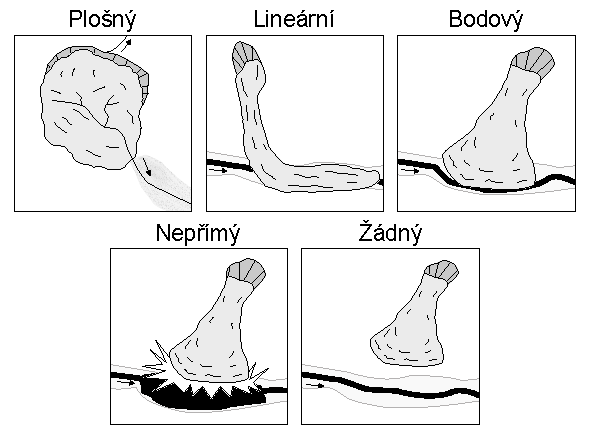
\includegraphics[width=1\linewidth]{obrazky/slope/korup_toky}
	\caption{Možné interakce mezi vodním tokem a sesuvem (upraveno podle \textcite{korupGeomorphicImprintLandslides2005})}
	\label{fig:koruptoky}
\end{figure}



\section{Eroze na svazích}

\subsection{Difuzní procesy}
Difuzní procesy jsou charakteristické tím, že se na transportu sedimentů nepodílí soustředěný tok vody, větru či ledu. Tyto procesy zahlazují nerovnosti na svahu a postupně snižují vertikální členitost reliéfu. 

\emph{Bombardování vodními kapkami} se uplatňuje zejména tam, kde \emph{vegetační kryt je velice řídký či zcela chybí} (pouště, badlandy). Vodní kapka, která dopadá na ukloněný povrch vymrští částečky, které letí proti a po svahu. Ty, které jsou odmrštěny proti svahu mají kratší trajektorii, než ty, které letí po svahu dolů. Tímto způsobem se tak materiál postupně přesouvá směrem po svahu. samozřejmě čím větší je sklon, tím delší je transport po svahu dolů.
%\todo[inline]{přidat obr. kapky}

Významnějším procesem je \emph{plošný (ronový) splach}. Jako \emph{ron} označujeme nesoustředěný odtok vody po povrchu. Největší účinky má plošný splach opět na svazích, které nejsou pokryté vegetací. K tomuto \emph{povrchovému odtoku} dochází při překročení infiltrační kapacity půdy nebo jejímu nasycení vodou. Se zvětšujícím se sklonem a narůstajícím množstvím vody se laminární proudění mění na turbulentní. To způsobuje soustředění odtoku a začátek hloubkové eroze, což v důsledku vede ke vzniku stružek a následně strží.

Do difuzních procesů se řadí i povrchové ploužení, ale o něm byla řeč již výše.

\subsection{Liniová eroze}
Soustředěním povrchového odtoku a vznikem turbulentního proudění dochází k intenzivní výmolné činnosti v místech soustředění. Iniciálním stádiem liniové eroze je \emph{stružková eroze}. \emph{Stružky} jsou mělké erozní rýhy, které jsou občasně protékané vodou. Většinou se jedná o systém paralelních pravidelně uspořádaných rýh. Vznikají v důsledku silných srážek nebo rychlého tání sněhu na vegetací nekrytých površích. 

Rozvojem stružek, jejich prohlubováním a prodlužováním do podoby, kdy jsou již trvalou součástí krajiny (např. jsou tak velké, že je nelze zaorat) vznikají \emph{strže}. Hovoříme pak o \emph{stržové erozi}. Strže mohou být občasně, ale i trvale protékané vodním tokem. 

\emph{Badland} je erozí zcela přemodelovaná plocha. Jedná se o hustou síť strží a stružek. Půda prakticky absentuje a vegetace je velice sporá. Badlandy často vznikají antropogenní příčinou. 

Intenzivní a člověkem urychlená eroze ze svahů (např. odlesněním, špatným hospodařením na polích) není problematická jen z důvodu ztráty půdy z daného místa a zmenšení obdělávatelných ploch. Materiál, který je odnesen se dostává do vodních toků, což snižuje kvalitu vody ale také materiál někde sedimentuje a to může způsobovat další problémy. 

\subsection{Sufoze}
\emph{Sufoze} je proces při kterém dochází k odnosu částic pod povrchem. Voda se dostává do podloží a následně soustavou drobných tunelů (\textit{pipes}) odtéká a odplavuje materiál. Sufoze nemusí být na povrchu patrná. Postupným zvětšováním tunelů ale následně může docházet ke kolapsům povrchů a vznikají \enquote{závrty}. V některých místech mohou tunely ústit na povrch a vytvářejí tak otevřené kanály, kde se na úpatí ukládá vyplavený materiál. Sufoze tak může předcházet následnému rozvoji strží. 

\newpage
\onecolumn
\begin{boxotazky}{Kontrolní a klíčové otázky, na které bychom měli znát odpověď}
	\begin{itemize}
		\item Jaké síly působí na svah? Jak jejich rozložení ovlivňuje sklon svahu?
		\item Jaké faktory ovlivňují stabilitu svahu?
		\item Co může snížit nebo naopak zvýšit stabilitu svahu?
		\item Jaké základní typy svahových pohybů existují?
		\item Jak moho sesuvy interagovat s vodními toky?
		\item Co to jsou difuzní procesy? Jaký mají efekt na svahu?
	\end{itemize}
\end{boxotazky}

\begin{boxslovnik}{Další klíčové pojmy k zapamatování}
	normálové a smykové napětí & pevnost ve smyku \\
	úhel vnitřního tření & koheze \\
	ron & sufoze \\
	
\end{boxslovnik}
\twocolumn

	\chapter{Fluviální procesy a formy reliéfu}
	%Vodní toky jsou významnou složkou krajiny. Potůčky, potoky, řeky odvádějí vodu z krajiny zpět do oceánů. Vodní toky jsou významným tvůrcem krajiny. Unášejí velké množství sedimentů a rozpuštěných látek. Podílejí se na denudaci
\section{Fluviální systém}
Vodní toky jsou jen jednou z částí \emph{fluviálního systému} (Obr. \ref{fig:fluvsystem}). Fluviální systém propojuje svahy, údolní nivy, říční síť a další části do jednoho celku, prostřednictvím kterého dochází k pohybu vody a sedimentů. Jelikož se jedná o otevřený systém, dochází k výměně energie a látek (vody, sedimentů) s jeho okolím. 

Hlavními vstupy do fluviálního systému jsou voda a sedimenty. Dalším vstupem může být například organický materiál (dřevo). Převážná část energie pohánějící celý systém pochází z atmosférických procesů (výpar, kondenzace, srážky). V podstatě zvyšují potenciální energii vody (dostává se do vyšších poloh). Díky gravitaci se pak voda dává do pohybu, tedy potenciální energie se mění na kinetickou. Část energie je pak vynaložena na transport sedimentů.

Výstup z fluviálního systému je zpravidla v místě ústí vodního toku do sedimentační pánve (jezero, moře, oceán...). 

Ve fluviálním systému dochází ale i k ukládání materiálu. Voda je v jezerech, vodních nádržích. Sedimenty jsou uložené v korytě, jezerech, nivách.

% TODO: \usepackage{graphicx} required
\begin{figure*}
	\centering
	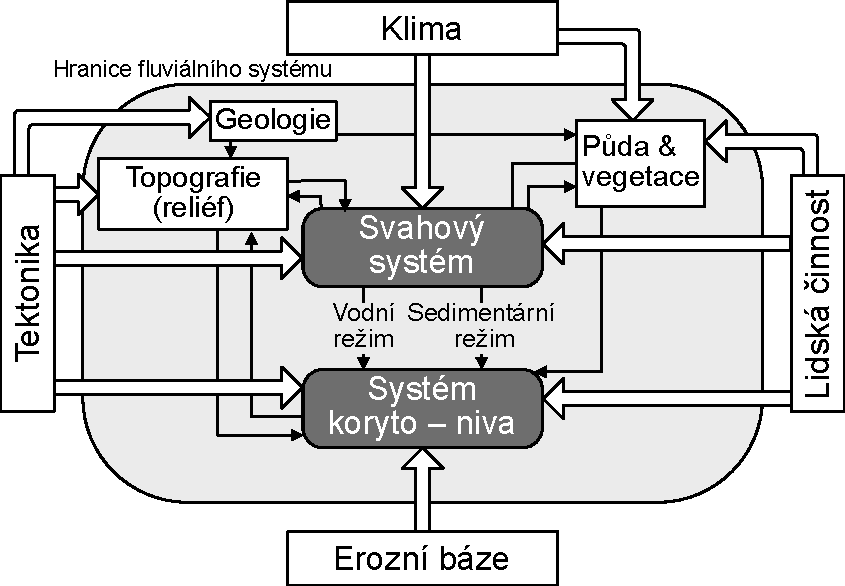
\includegraphics[width=0.9\linewidth]{obrazky/fluvial/fluv_system}
	\caption{Zjednodušené schéma fluviálního systému (upraveno podle \textcite{charltonFundamentalsFluvialGeomorphology2007}.)}
	\label{fig:fluvsystem}
\end{figure*}

\section{Proudění vody v korytech}
Proudění je neuspořádaný pohyb částic tekutiny (vody) převážně jedním směrem. Díky gravitaci teče voda v korytech shora dolů. Tomuto pohybu brání tření na rozhraní voda-koryto, ale i vnitřní tření vlastní vody. 

Proudění může být \emph{ustálené} neboli stacionární (\textit{steady flow}). Při tomto typu proudění se částice pohybují jedním směrem a se stále stejnou rychlostí -- průtok se nemění.  Opakem je \emph{neustálené proudění} neboli nestacionární (\textit{unsteady flow}), kdy se rychlost v závislosti na čase mění.

\emph{Rovnoměrné (uniformní) proudění} (\textit{uniform flow}) je ustálené proudění, při kterém jsou konstantní další parametry toku (např. průtočná plocha). Při \emph{nerovnoměrném proudění} (\textit{non-uniform flow}) se průtok nemění, ale mění se rychlost proudění, průtočná plocha a další parametry. 

\subsection{Charakter proudění v korytech}
\emph{Laminární proudění} je takové proudění, kdy se kapalina pohybuje ve vrstvách -- laminách, které navzájem kloužou po sobě (Obr. \ref{fig:laminarturbul}). Laminárním prouděním jsou typické vysoce viskózní kapaliny. Jelikož voda má malou viskozitu, laminární proudění se projevuje jen při nízkých rychlostech.
\emph{Turbulentní proudění} je chaotické a všesměrné (Obr. \ref{fig:laminarturbul}). Pohyb je realizován po i proti proudu, do stran, nahoru či dolů. 

% TODO: \usepackage{graphicx} required
\begin{figure}[h]
	\centering
	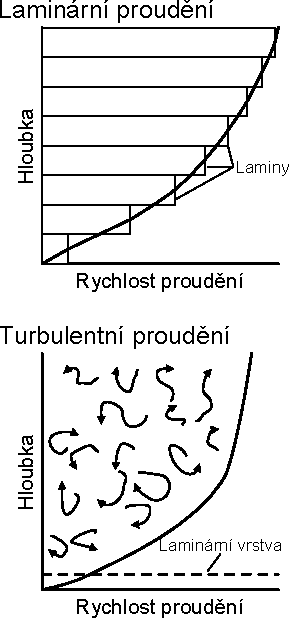
\includegraphics[width=1\linewidth]{obrazky/fluvial/laminar_turbul}
	\caption{Laminární a turbulentní proudění.}
	\label{fig:laminarturbul}
\end{figure}


\emph{Reynoldsovo číslo} vyjadřuje, zda proudění bude laminární nebo turbulentní. Jedná se o bezrozměrné číslo, které je dáno poměrem inertních sil a viskózních sil.

\begin{equation}\label{key}
	Re = \frac{\text{Inerční síly}}{\text{viskózní síly}} = \frac{vR}{\nu_{s}}
\end{equation}

\begin{eqexpl}
	\item{$Re$}Reyonoldsovo číslo (bezrozměrné)
	\item{$v$}Rychlost proudění [\si{\metre\per\second}]
	\item{$R$} je hydraulický poloměr [\si{\metre}]
	\item{$\nu_{s}$} je kinematická viskozita [\si{\metre\squared\per\second}]
\end{eqexpl}

Laminární proudění je do hodnoty $Re$ < $500$ při hodnotách $Re$ = $500$ -- $1000$ má proudění přechodný charakter. Turbulentní proudění má hodnoty $Re$ > $2000$.

Na základě \emph{Froudeho čísla ($Fr$)} rozdělujeme proudění na \emph{bystřinné} a \emph{říční}. Pokud je $Fr >1$ jedná se proudění \emph{bystřinné} neboli \emph{nadkritické} (\textit{supercritical flow}). V případě $Fr <1$ jde o \emph{říční (podkritické) proudění} (\textit{subcritical flow}). $Fr = 1$ značí \emph{kritické} proudění. Froudeho číslo je závislé na rychlosti a hloubce proudění:

\begin{equation}
	Fr=\frac{v}{\sqrt{gd}}
\end{equation}

\begin{eqexpl}
	\item{$Fr$} Freudeho číslo (bezrozměrné)
	\item{$v$} Rychlost proudění [\si{\metre\per\second}]
	\item{$g$} tíhové zrychlení [\SI{9,81}{\metre\per\second\squared}]
	\item{$d$} hloubka proudění [\si{\metre}]
\end{eqexpl}

Ve většině případů je i v horských bystřinách říční proudění. Bystřinné (nadkritické) proudění se vyskytuje jen lokálně. Nadkritické proudění je charakteristické menším turbulentním promícháváním vody, což způsobuje efektivnější a rychlejší tok korytem. Přechod mezi podkritickým a nadkritickým prouděním se na toku projevuje hydraulickým poklesem. V opačném případě, kdy dochází ke změně proudění ze nadkritického na podkritické, vzniká hydraulický skok. 
%\todo[inline]{obrázek hydraulický skok, pokles}

\subsection{Rychlost proudění, průtok}
Rychlost proudění vody v korytě je závislá na několika faktorech. Velký vliv má samozřejmě sklon koryta, kdy s zvětšujícím se sklonem roste i rychlost proudění. Jelikož je pohyb vody bržděn třením o dno a břehy, velice důležitým faktorem je \emph{relativní drsnost koryta}. Čím je menší relativní drsnost koryta (a tedy i výsledné tření), tím větší je rychlost proudění. Drsnost koryta je relativní vůči hloubce proudění (hloubce toku). Stejné koryto bude mít větší relativní drsnost při nízkých průtocích, než při vysokých. Představte si tok s minimálním průtokem, kde si voda hledá cestičky mezi valouny a to samé koryto za vyššího vodního stavu. Jednotlivé valouny, které při nízkém průtoku čněly nad vodu již na celkovou drsnost budou mít pramalý vliv. Při větší hloubce toku je totiž jen menší část ovlivněna třením na rozhraní voda-koryto. 

Z důvodu tření pozorujeme nejnižší rychlosti proudění u břehů a dna. Směrem k hladině rychlost proudění nelineárně narůstá. Maxima jsou kousek pod hladinou, jelikož na hladině dochází k tření vody o vzduch a také tam jsou přítomné víry, které proudění zpomalují.

\emph{Průtok} je definován jako objem vody, která proteče profilem vodního toku za jednotku času. Typicky je průtok vyjadřován v \si{\metre\cubed\per\second}. 
\begin{equation}
	Q=vA
\end{equation}
\begin{eqexpl}
	\item{$Q$} Průtok [\si{\metre\cubed\per\second}]
	\item{$v$} Rychlost proudění [\si{\metre\per\second}]
	\item{$A$} Průtočná plocha příčného profilu [\si{\metre\squared}]
\end{eqexpl}


\emph{Manningova rovnice} vyjadřuje vztah mezi rychlostí proudění v korytě a parametry koryta:
%Manningova rovnice
\begin{equation}\label{eq:manning}
	v = [R^{\nicefrac{2}{3}}S^{\nicefrac{1}{2}}]/n
\end{equation}

\begin{eqexpl}
	\item{$v$} rychlost proudění [\si{\metre\per\second}]
	\item{$R$} hydraulický poloměr [\si{\metre}]
	\item{$S$} sklon vodní hladiny[\si{\metre\per\metre}]
	\item{$n$} Manningův koeficient drsnosti [bezrozměrné]
\end{eqexpl}

% Please add the following required packages to your document preamble:
% \usepackage{booktabs}
\begin{table*}[]
	\begin{tabularx}{1\textwidth}{@{}Xlll@{}}
		\toprule
		Popis koryta                                                    & Minimum & Běžná hodnota & Maximum \\ \midrule
		Rovné koryto bez vegetace                                       & 0,025   & 0,030         & 0,033   \\
		Klikatící se koryto bez vegetace s občasnými tůněmi a mělčinami & 0,033   & 0,040         & 0,045   \\
		Klikatící se koryto s vegetací a kameny na dně                  & 0,035   & 0,045         & 0,050   \\
		Hodně zarostlé koryto s hlubokými tůněmi                        & 0,075   & 0,100         & 0,150   \\
		Horské toky, na dně štěrky, valouny, balvany občasně            & 0,030   & 0,040         & 0,050   \\
		Horské toky; valouny a velké balvany                            & 0,040   & 0,050         & 0,070  \\ \bottomrule
	\end{tabularx}
	\caption{Manningovy koeficienty drsnosti $n$ pro malé toky (šířka do \SI{30}{\metre}). Zdroj: \textcite{chowOpenchannelHydraulics1959}}
	\label{tab:manning}
\end{table*}

\section{Energie, práce a výkon vodních toků}
Pohyb vody, sedimentů, eroze. To vše zahrnuje vykonávání \emph{práce}, tedy působení síly na hmotu po určité dráze. \emph{Energie} z vyjadřuje schopnost hmoty konat práci. Hmota s větší potenciální energií má větší kapacitu konat práci. Jak práce, tak energie mají stejnou jednotku -- jouly [\si{\joule}]. \emph{Výkon} vyjadřuje množství vykonané práce za jednotku času, jednotka je joul za sekundu neboli watt [\si{\watt}].

Pohybem vody z vyšších nadmořských výšek do nižších se přeměňuje potenciální energie vody na kinetickou (Rov. \ref{eq:potkin}). Až $95 \%$ kinetické energie se třením přemění na teplo. Zbylá energie je transformována na samotný pohyb vodní masy, transport sedimentů, erozi dna a břehů. Malý zlomek energie je vynaložen na zvukové projevy. 

\begin{equation}\label{eq:potkin}
	\underset{\text{potenciální energie}}{mgh} \longrightarrow \underset{\text{kinetická energie}}{\frac{1}{2}m v^{2}}
\end{equation}

\begin{eqexpl}
	\item{$m$} hmotnost vody [\si{\kilo\gram}]
	\item{$g$} tíhové zrychlení [\si{\metre\per\second\squared}]
	\item{$h$} relativní výška [\si{\metre}]
	\item{$v$} je rychlost proudění[\si{\metre\per\second}]
\end{eqexpl}

Výkon vodních toků se měří ve wattech na jednotku délky [\si{\watt\per\metre}] a vyjadřuje kapacitu vodního toku transportovat sedimenty. \emph{Výkon vodního toku} ($\Omega$) je hlavně závislý na průtoku ($Q$) a jeho sklonu ($S$).

\begin{equation}\label{eq:vykontoku}
	\Omega = \rho g Q S
\end{equation}

\begin{eqexpl}
	\item{$\Omega$} výkon vodního toku [\si{\watt\per\metre}]
	\item{$\rho$} hustota vody [\si{\kilogram\per\metre\cubed}]
	\item{$Q$} průtok [\si{\metre\cubed\per\second}]
	\item{$S$} je sklon vodní hladiny[\si{\metre\per\metre}]
\end{eqexpl}

Často se používá \emph{specifický výkon toku}, který je definován jako podíl výkonu toku ($\Omega$) a šířky koryta ($W$): 

\begin{equation}\label{eq:spec_vykon}
	\omega = \frac{\Omega}{W}
\end{equation}

Odpadá tím vliv šířky toku na výkon a lze tak jednoduše srovnávat toky mezi sebou. 

Proudící voda v korytě působí na dno \emph{tečným neboli smykovým napětím} (\textit{shear stress}). Pro ustálené rovnoměrné proudění je toto tečné napětí definované takto:

\begin{equation}\label{eq:tecne}
	\tau_{b} = \rho g R S
\end{equation}

\begin{eqexpl}
	\item{$\tau_{b}$} tečné napětí [\si{\newton\per\metre\squared}]
	\item{$\rho$} hustota vody [\si{\kilogram\per\metre\cubed}]
	\item{$R$} Hydraulický poloměr [\si{\metre}]
	\item{$S$} je sklon vodní hladiny[\si{\metre\per\metre}]
\end{eqexpl}

Vztah mezi specifickým výkonem toku, tečným napětím ($\tau_{b}$) a průměrnou rychlostí v profilu ($\bar{v}$) je následovný:

\begin{equation}\label{eq:spec_vykon_tecne}
	\omega = \tau_{b} \bar{v}
\end{equation}

\section{Fluviální eroze}
Fluviální eroze je výsledkem celé řady procesů a faktorů, které se uplatňují. 

\subsection{Typy eroze}
Erozi dělíme podle směru jejího působení. Při \emph{lineární (hloubkové) erozi} řeka prohlubuje své koryto. Dochází k erozi říčního dna. Při \emph{boční (břehové, laterální) erozi} dochází k pohybu toku do stran a erozi břehů. Jako \emph{zpětnou erozi} označujeme zahlubování vodního toku, které postupuje proti proudu. Zahlubování začalo v nižších polohách a postupuje do vyšších nadmořských výšek. Stává se, že erozně aktivnější vodní tok (s intenzivní zpětnou erozí) se napojí na vodní tok z jiného povodí. Tomuto jevu se říká \emph{říční pirátství}. Intenzivněji erodující tok zvětší své povodí na úkor jiného toku. 

%\todo[inline]{eroze, říční pirátství}

\subsection{Erozní procesy}

\subsubsection{Eroze ve skalních korytech}
Jelikož dotace sedimentů do skalních koryt je často omezená, jejich podoba je dána hlavně erozní činností vody. 

Proudící voda může erozně půdobit několika způsoby. \emph{Koroze} je proces chemického rozpouštění na kontaktu proudící vody a podloží. INtenzita koroze je závislá na rozpustnosti podloží, nasycenosti vody, průtokem a rychlostí proudění. Koroze je důležitým procesem ve vápencových oblastech.

\emph{Abraze (koraze)} je proces mechanického působení a odnosu podloží koryta v důsledku působení transportovaných částic. Účinek abraze závisí na množství a velikosti částic, jejich kinetické energii a odolnosti podloží. Rychlost proudění má velký účinek, neboť kinetická energie se mění se čtvercem rychlosti. 

Samotná proudící voda působí mechanicky na podloží. Tlakem vodního proudu může vytrhávat zvětralé podloží (tzv. \emph{plucking}). Intenzivnější je \emph{kavitace}. Jedná se o erozní činnost explodujících vzduchových bublin ve vodě. Intenzivně se plucking projevuje u vodopádů a peřejí. Třetím typem je mechanického působení je \emph{evorze}, což je mechanické působení turbulentního proudění. Jeho působením vznikají evorzní prohlubně -- \emph{obří (evorzní) hrnce}.

\subsubsection{Eroze v aluviálních korytech}
Aluviální koryta jsou charakteristická hlavně boční erozí. Ta je mimo jiné závislá na charakteru materiálu tvořící břehy. Významný stabilizační efekt má vegetace.

Břehová eroze je výsledkem různých procesů. \textcite{charltonFundamentalsFluvialGeomorphology2007} je dělí do tří skupin:
\begin{enumerate}
	\item \emph{Přípravné oslabující procesy} jako je například namáčení a vysoušení materiálu. Procesy činící břeh náchylným k erozi.
	\item \emph{Fluviální procesy}, kdy jednotlivé částice a agregáty jsou uvedené do pohybu vodou.
	\item \emph{Svahové procesy} zahrnující kolaps břehů (sesuvy, břehové nátrže)
\end{enumerate}

Nízké ale strmé břehy tvořené kohezním materiálem řasto kolabují odkláněním (topplingem), kdy se blok překlopí do koryta (Obr. \ref{fig:bankerosion}a). Odlučná plocha je téměř vertikální. U vyšších ale méně strmých břehů vznikají v kohezních materiálech rotační sesuvy (Obr. \ref{fig:bankerosion}b). U břehů tvořených nekohezním materiálem převažují mělké sesuvy, nátrže a opad (Obr. \ref{fig:bankerosion}c). Často jsou břehy z nekohezního materiálu v podloží a jemného kohezního materiálu v nadloží. Erozí méně odolného nekohezního materiálu dochází k podemílání břehu a jeho následného kolapsu (Obr. \ref{fig:bankerosion}).

\begin{figure}
	\centering
	\includegraphics[width=1\linewidth]{obrazky/fluvial/bank_erosion}
	\caption{Procesy břehové eroze. Upraveno podle \textcite{charltonFundamentalsFluvialGeomorphology2007}}
	\label{fig:bankerosion}
\end{figure}

\subsection{Zdroje sedimentů}
Hlavním zdrojem sedimentů jsou svahy v povodí. Rychlost tvorby svahoviny, která se následně může dostávat do vodního toku je dána geologickou stavbou (litologií, geologickou strukturou), klimatickými podmínkami. Donášku sedimentů do toku ale i významně ovlivňuje i vegetace. 

V horských oblastech, kde svahy jsou strmé, se do koryta snadněji budou dostávat klasty větších rozměrů. V nížinných oblastech pak převažuje plošný splach jemných sedimentů. Významným zdrojem sedimentů jsou břehové nátrže. 

\section{Fluviální transport}
\subsection{Uvedení částic do pohybu}
Co je potřeba, aby vodní tok uvedl do pohybu jednotlivé klasty? Klast ležící na dně je pod vlivem sil, které jej chtějí uvést do pohybu a těch, které ho drží na místě. Pokud mobilizační síly převáží, klast se dá do pohybu (Obr \ref{fig:sily_klast}). Proti pohybu působí tíha částice (normálová komponenta) a také okolní klasty, které mohou danou částici blokovat. Proudící voda působí na klast silou, kterou lze rozdělit do dvou složek. \emph{Vztlaková síla} (\textit{lift}) působí směrem vzhůru. \emph{Tření} (\textit{drag force}) působí ve směru proudění. 

\begin{figure}
	\centering
	\includegraphics[width = 1\linewidth]{obrazky/fluvial/sily_klast}
	\caption{Síly působící na klast ve vodním toku \textcite{summerfieldGlobalGeomorphologyIntroduction1999}).}
	\label{fig:sily_klast}
\end{figure}

Kromě velikosti, hustoty, tvaru klastu hraje při jeho mobilizaci i to, jak je vystaven toku a také na rychlosti proudění nebo přesněji na kritickém tečném napětí. Tzv. Hjulstr\o{}mův diagram (Obr. \ref{fig:hjulstr}) znázorňuje při jakých rychlostech proudění se částice o dané velikosti začne pohybovat (je vodním tokem stržena), zůstává v pohybu a nebo sedimentuje. Tento diagram vznikl na základě laboratorních experimentů a ve volné přírodě jsou tyto vztahy složitější. Jak je z diagramu patrné, tak nejsnáz jsou erodované částice písku okolo \SIrange{0,1}{0,5}{\milli\metre}. Jílové částice jsou drženy pospolu kohezními silami, proto jsou nutné vyšší rychlosti proudění pro jejich uvedení do pohybu. 

\begin{figure*}
	\centering
	\includegraphics[width = 1\textwidth]{obrazky/fluvial/hjulstr}
	\caption{Hjulstr\o{}mův diagram znázorňující vztah mezi velikostí částice, rychlostí proudění a procesem (upraveno podle \textcite{hjulstromStudiesMorphologicalActivity1935})}
	\label{fig:hjulstr}
\end{figure*}

\begin{figure*}
	\centering
	\includegraphics[width = 1\textwidth]{obrazky/fluvial/lanes_balance.jpg}
	\caption{Bilance mezi paramtry koryta, sedimenty, průtokem (převzato z \textcite{dustConceptualModelComplex2012})}
	\label{fig:vahy}
\end{figure*}

\subsection{Způsob fluviálního transportu}
Vodní toky transportují materiál ve dvou základních podobách -- rozpuštěný ve vodě a v pevném skupenství (klastický materiál) (Obr. \ref{fig:fluvsedtrans}). 

Klastický materiál transportovaný v suspenzi nazýváme \emph{plaveniny} (\textit{suspended load}).  V celém profilu vodního toku je koncentrace plavenin stejná, což je způsobené turbulentním prouděním. Plaveniny způsobují zakalení vody. V suspenzi je unášena většina ($70 \%$) z celosvětového množství unášeného materiálu řekami. V nížinných tocích plaveniny tvoří \SIrange{70}{95}{\percent} celkového objemu transportovaných sedimentů, bystřinné a štěrkonosné toky mají velké rozpětí (\SIrange{20}{90}{\percent}) závislé na dodávce hrubšího materiálu. 

\emph{Dnové splaveniny} (\textit{bed load}) jsou sedimenty, které se pohybují v kontaktu se dnem. Jednotlivé klasty se mohou sunout, válet se, nebo se pohybují poskákováním -- saltací. Dnové splaveniny mají velký geomorfologický efekt na koryto. S délkou transportu se zvětšuje opracování jednotlivých klastů (z ostrohranných se stávají zaoblené). Obecně také platí, že s délkou transportu a s délkou vodního toku se zmenšuje průměr částic.

\begin{figure}
	\centering
	\includegraphics[width = 1\linewidth]{obrazky/fluvial/fluv_sed_trans}
	\caption{Fluviální transport klastických sedimentů. Rozpuštěné látky nejsou zobrazeny (upraveno podle \textcite{charltonFundamentalsFluvialGeomorphology2007}).}
	\label{fig:fluvsedtrans}
\end{figure}

\emph{Rozpuštěný materiál} (\textit{dissolved load}) je transportovaný v roztoku (např. ionty \ce{Ca^2+}, \ce{Mg^2+}, \ce{Na+}, \ce{SiO2}, \ce{HCO3-}, živiny na bázi fosforu, dusíku, rozpuštěné plyny. Globálně rozpuštěné látky odpovídají přibližně $20 \%$ celkové denudace. Koncentrace látek klesá s rostoucím průtokem. Morfologický efekt rozpuštěných látek na koryto je malý. 


\section{Říční koryto}
\subsection{Typy říčních koryt}
Rozlišují se tři typy říčních koryt. \emph{Aluviální} koryta jsou tvořena říčními sedimenty. \emph{Skalní} koryta jsou opakem aluviálních. Nachází se v nich minimální množství sedimentů a řeka je zahloubená do skalního podloží. Oba typy koryt ale nejsou ostře ohraničená, existuje tak \emph{přechodný typ}. 

\subsubsection{Skalní koryta}
Skalní koryta jsou  zařezaná do skalního podloží. To je činí poměrně stabilními. K bočním posunům koryta dochází v málo odolných horninách. Skalní koryta jsou zpravidla v horních částech toku, kde je větší sklon a řeka unáší hrubší materiál. Podélné profily skalních koryt jsou zpravidla nevyrovnané s velkým množstvím zálomů, tzv. knickpointů. Tyto zálomy jsou v místech, kde se dramaticky mění sklon koryta respektive je tam přítomen nějaký skok. Tento skok může být způsoben zlomem, mohou ho způsobovat sesuvy, které mohou zahradit údolní dno. 

\emph{Zakleslé meandry} (\enquote{intrenched meanders}) se nachází v místěch horizontálně uložených vrstev. Meandrující řeka se postupně zařezává do aluvia a postupem času se začne zakusovat i do skalního podloží. 

\subsubsection{Aluviální koryta}
Jak již bylo řečeno, aluviální koryta jsou tvořena vlastními říčními sedimenty. Tento typ koryt je velice různorodý, což je dáno variabilitou průtoku; množstvím, typem unášeného a ukládaného materiálu apod. Zároveň je tento typ koryt citlivý na změny v dodávkách sedimentů -- jejich množství a hrubosti, změny v průtoku, jelikož aluviální sedimenty snadno podléhají erozi. 

\subsubsection{Přechodná koryta}
Do kategorie spadající mezi aluviální a skalní koryta patři ty, které jsou lokálně ovlivněny skalním podložím případně jsou v aluviu odolném vůči erozi.

\subsection{Geometrický vzor toku}
Na rozdíl od skalních koryt mohou koryta v aluviu nabývat celé řady podob. Rozlišujeme několik základních vzorů. 

Podle sinuosity (poměr mezi délkou koryta k délce údolnice) rozlišujeme:

\begin{itemize}
	\item Přímá koryta
	\item Koryta se zákruty a meandry
	\item Divočící koryta
	\item Anastomózní koryta
\end{itemize}

\subsubsection{Přímé toky}
Čistě přímá aluviální koryta nejsou běžná. Zpravidla jsou vázaná na rovné úseky \enquote{V-údolí}, které jsou vázané na strukturní predispozice. Přímé toky v nížinách jsou zpravidla vždy výsledkem antropogenních úprav koryta. 

\subsubsection{Meandrující toky}
Meandrující toky jsou patrně nejrozšířenější formou. Jedná se o řeky, které se rozličně klikatí krajinou. Meandrující toky mají sinusoitu větší než $1,5$ \parencite{huggettFundamentalsGeomorphology2017}. Vlnová délka meandrů jsou přímo závislé na šířce koryta. Větší toky mají i větší vlnovou délku meandrů. Do tohoto vztahu vstupují ale i další faktory jako je například materiál aluvia. 

Meandry vznikají rozkmitáním proudnice a díky přítomnosti sekundárního tzv. heliakálního proudění. Toto proudění zvyšuje erozi na nárazovém \emph{výsepním} břehu a napomáhá sedimentaci na vnitřním \emph{jesepním} břehu. 

\begin{figure}
	\centering
	\includegraphics[width=1\linewidth]{obrazky/fluvial/mendry_sinusoita}
	\caption{Sinusoita koryta a geometrické parametry meandrů (upraveno podle \textcite{biermanKeyConceptsGeomorphology2014})}
	\label{fig:mendrysinusoita}
\end{figure}

\subsubsection{Divočící toky}
Vodní tok, který nese velké množství hrubého materiálu (štěrku) a má hodně rozkolísané průtoky vytváří tzv. divočící tok. Tento typ toků se nachází při vyústění horských toků do předpolí. Tok přetížený sedimenty je začne ukládat. Vznikají štěrkové lavice -- akumulace, které tok různě obtéká, větví se na nich. Typické je časté překládání koryta. Z důvodu velké dynamiky lavic se vegetace nestačí uchytit na štěrkových lavicích a stabilizovat je.

\begin{figure}[h]
	\centering
	\includegraphics[width=1\linewidth]{obrazky/fluvial/divocici}
	\caption{Divočící řeka Waimakariri, Nový Zéland (Autor: Greg O'Beirne CC BY-SA 3.0)}
	\label{fig:divocici}
\end{figure}

\subsubsection{Větvící se toky}
Jedná se o přechodný typ mezi divočícím a jednoduchým (nevětvícím se) tokem. Větvící se toky mají zpravidla hlavní koryto a menší vedlejší koryta. V některých případech se jedná jen o povodňová (tzv. avulzní koryta). Štěrkové lavice větvících se toků bývají stabilnější a porostlé dřevinnou vegetací \parencite{galiaFluvialniGeomorfologie2017}.
%Při vyústění horských toků s rozkolísanými průtoky na předpolí
%Předpoklady:
%\begin{itemize}
%	\item Velké množství sedimentů
%	\item Snadno erodovatelné břehy
%	\item Velká rozkolísanost průtoků
%	\item Velký gradient údolí
%	\item Časté laterární změny v půdorysu spojené s nestabilními koryty a velkým množstvím dnových splavenin
%	\item Vznik a překládání štěrkových lavic, ostrovů atd.
%\end{itemize}

\subsection{Anastomózní toky}
Půdorysně podobné divočícímu toku jsou \emph{anastomózní toky} (\textit{anastomosed} nebo \textit{anabranching channels}). Tento typ vodního toku ale není tvořen jedním korytem členěným do celé řady větví měnících se v čase. Anastomózní tok je soustava sinusouidních až meandrujících koryt, které jsou mírně zahloubené do nivy. Vzniklé říční ostrovy jsou stabilní a porostlé vegetací. Anastomźní toky se nacházejí v nížinách.


\section{Údolí}

Tvar údolí je výsledkem vztahu mezi lineární erozí vodního toku a vývojem svahů.

\emph{Soutěsky} (hluboké soutěsky = kaňony), vznikají při převaze lineární eroze. Svahy soutěsky jsou zhruba rovnoběžné a šířka je přibližně stejná ve spodní i horní části.

\emph{Údolí ve tvaru písmene V} vznikají při rovnováze mezi zahlubováním toků a vývojem svahů. Dno údolí je tvořeno korytem vodního toku a směrem nahoru se údolí rozevírá. 

\emph{Neckovitá údolí} vznikají při převaze boční eroze vodního toku nad hloubkovou. Meandrováním vodního toku dochází k podemílání svahů tu na jedné, tu na druhé straně údolí. Vzniká údolí s širokým dnem, které je zpravidla zaplněné údolní nivou. Údolní dno přechází ostrým zálomem dno relativně příkrých svahů. 

\emph{Úvalovité údolí} je údolí se širokým dnem, které bez výrazného zálomu přechází do mírných svahů.

\begin{figure}[h]
	\centering
	\includegraphics[width=1\linewidth]{obrazky/fluvial/typy_udoli}
	\caption{Typy údolí. A) údolí typu "V", B) soutěska, C) neckovité údolí, D) úvalovité údolí}
	\label{fig:typyudoli}
\end{figure}

\subsection{Vodní toky a morfostruktura}
Vodní lze rozdělit podle jejich vztahu k morfostrukttuře. \textcite{demekObecnaGeomorfologie1987} rozlišuje \emph{konsekventní toky}, které mají směr toku určený původním sklonem georeliéfu. Tento typ vodních toků zpravidla není závislý na morfostruktuře. \emph{Subsekventní toky} jsou vázané na méně odolné horniny nebo na tektonické linie. Jejich směr je shodný se směrem a úklonem vrstev nebo shodný s průběhem tektonických linií. \emph{Resekventní toky} mají stejný směr jako konsekventní. Nacházejí se ale na erozním případně strukturním povrchu nižší úrovně než konsekventní toky. \emph{Obsekventní toky} mají směro opačný než je generelní sklon povrchu krajiny. Tento typ toků je často vázán na tektonické linie. \emph{Insekventní toky} nejsou nijak závislé na morfostruktuře či původním sklonu.

Rozlišují se i specifická průlomová údolí. \emph{Antecedentní údolí} vzniká tehdy, když se vodní tok zařezává do postupně se vyzdvihujícího se území. Je ale potřeba, aby výzdvih byl celkově pomalejší, než hloubková eroze toku. \emph{Epigenetické údolí} vzniká zařezáváním do měkkého podloží, kde i po dosažení odolnějších hornin dojde k zachování směru toku. 


\subsection{Podélný profil a erozní báze}
Podélný profil (\textit{longitudal profile}) vodního toku (také spádová křivka vodního toku) zobrazuje jak se mění nadmořská výška toku se vzdáleností od pramene k ústí. Ideální tzv. \emph{vyrovnaný podélný profil} je konkávní a hladký (bez různých zálomů). V horní části vodního toku je křivka nejstrmější a směrem k ústí se zmírňuje. Tento \enquote{ideální} vodní tok neeroduje své podloží ani neakumuluje sedimenty. Je totiž schopen veškerý materiál, který se do něj dostane např. svahovými procesy, transportovat. K vyrovnanému podélnému profilu spějí veškeré vodní toky. Je včak nedostižným ideálem, protože do vývoje podélného profilu zasahuje celá řada faktorů jako je odolnost hornin, donáška sedimentů, tektonické pohyby, změny v průtoku apod. 

S podélným profilem vodního toku je třeba zmínit i \emph{erozní bázi}. Erozní báze je místo o určité nadmořské výšce pod kterou se vodní tok nedokáže zahlubovat případně se zahlubuje jen velice obtížně. \emph{Globální erozní bází} je hladina světového oceánu. \emph{Lokální erozní bází} může být ústí vodního toku do větší řeky, jezera. Může to být ale vrstva odolných hornin nebo antropogenní prvek v korytě jako je jez.




%\todo[inline]{podélný profil, erozní báze}
%\todo[inline]{vztah ke struktuře}

\section{Korytové formy}
Sediemnty unášené vodním tokem vytvářejí celou řadu různých více či méně trvanlivých forem. Při rovnováze mezi donáčkou sedimentů a transportní kapacitou toku vzniká na dně štěrkonosných toků vrstva tvořená z hrubšího materiálu, než je pod povrchem. Dochází i k \emph{imbrikaci}, což je uspořádání klastů (štěrků, valounů) tak, aby jejich nejdelší osa byla kolmá na směr proudění a nejkratší osa kolmá na dno toku. Imbrikované klasty jsou odolnější vůči erozi - vzniká \emph{armovaná vrstva}.

Typickým tvarem vodních toků s písečným dnem jsou \emph{čeřiny a duny} (\textit{dunes, ripples}). Jedná se o mobilní korytové formace. Čeřiny vznikají již pri velice nízkých rychlostech proudění. Duny vznikají při vyšších rychlostech. 

Z větších klastů jsou tvořené \emph{sedimentární klastry} (\textit{particle clusters}). Jedná se o shluky štěrků či valounů, uložených nad a pod základním (největším) valounem (Obr. \ref{fig:klastklastr}). 

\begin{figure}
	\centering
	\includegraphics[width=1\linewidth]{obrazky/fluvial/klast_klastr}
	\caption{Znázornění sedimentárního klastru. Upraveno podle \textcite{galiaFluvialniGeomorfologie2017})}
	\label{fig:klastklastr}
\end{figure}

Běžným tvarem, který nacházíme v korytě jsou \emph{štěrkové a písčité lavice} (Obr. \ref{fig:lavice}). Jedná se o nánosy štěrku (písku). Vznikají v rozličných pozicích a z různých příčin. Obecně se dá ale říct, že hlavním důvodem jejich vzniku je ztráta unášecí schopnosti toku. \emph{Střídavé lavice} se nacházejí (\textit{alternat bars}) střidavě u jednoho a u druhého břehu. Vznikají během sestupné fáze povodňové vlny (při klesajícím vodním stavu). Střídavé lavice způsobují rozkmitání proudnice. Na soutocích můžeme spatřit \emph{soutokové lavice} (\textit{channle junction bars}). \emph{Diagonální lavice} (\textit{diagonal bars}) procházejí šikmo korytem. Vznikají v místech rozšíření koryta, kde vodní tok ztrácí energii nebo je v daném místě větší donáška sedimentů. \emph{Středové lavice} (\textit{mid-channel bars}) mohou vnzikat z diagonálních. Nacházíme je v divočících tocích. \emph{Vrcholové lavice} (\textit{point bars}) se nacházejí na vnitřní (akumulační) straně meandru jako důsledek pomalejšího proudění a působení sekundárních proudů.

% TODO: \usepackage{graphicx} required
\begin{figure}
	\centering
	\includegraphics[width=1\linewidth]{obrazky/fluvial/lavice}
	\caption{Příklad některých lavic, které lze nalézt v říčním korytě. A vrcholové lavice, B střídavé lavice, C středové lavice (bermy), D lavice před překážkou, E nepravidelné lavice, F lavice v divočícím toku  (upraveno podle \textcite{radecki-pawlikStreamHydraulicsGranulometry2004} }
	\label{fig:lavice}
\end{figure}

\section{Mimokorytové formy}
\subsection{Niva}
\emph{Niva} (\textit{floodplain}) je akumulační plošina v okolí vodního toku, která je pravidelně zaplavována. Nivu najdeme v okolí většiny řek. Výjimku tvoří toky v horském prostředí, které mají vysokou transportní kapacitu, a kde v sevřených údolích není prostor pro její vývoj. Šířka nivy se zpravidla odvíjí od velikosti řeky, jejího průtoku. Mohutnější řeka bude mít širší nivu, než její menší přítoky. 

Ukládání sedimentů v nivě probíhá vertikální a boční akrecí. K \emph{vertikální akreci} dochází při rozlití vody do nivy při povodňové události. Voda v důsledku větší drsnosti nivy proudí pomaleji, což snižuje její schopnost transportovat sedimenty a ty se ukládají na povrch nivy. Jejich množství a zrnitost klesá směrem od koryta. Důsledkem této nerovnoměrné distribuce sedimentů v nivě je vznik \emph{agradačních (břehových) valů} (\textit{levees}) kolem koryta. Jsou tvořeny hlavně písčitými sedimenty a mohou mít výšku v řádu decimetrů až několika metrů. Ve větší vzdálenosti od koryta se ukládá jemnozrnnější materiál (prach, jíl), což označujeme jako facii \emph{povodňových hlín}. \emph{Boční (laterální) akrece} je výsledkem migrace toku do stran. Typické je posouvání meandrů, kdy na vnitřní straně dochází k ukládání vrcholové štěrkové lavice. Ta tvoří tzv. \emph{korytovou facii}. Protrhnutím meandrové šíje vznikají slepá a mrtvá ramena. Ty mají specifické sedimenty s velkým obsahem organické hmoty -- \emph{facie opuštěných koryt}.

%\todo[inline]{obrázek nivy akrece}

\begin{figure}[h]
	\centering
	\includegraphics[width=1\linewidth]{obrazky/fluvial/meander}
	\caption{Meandrující řeka. (USGS, volné dílo)}
	\label{fig:meander}
\end{figure}

\subsection{Říční terasy}
\emph{Říční terasy} (\textit{river terraces}) jsou zbytky údolních den, které se nacházejí v různých výškách nad současným vodním tokem. Vznikly v důsledku zahloubení toku. Říční terasa se skládá z plošiny terasy a terasového stupně. \emph{Plošina terasy} je zbytek povrchu staré nivy. \emph{Terasový stupeň (svah)} odděluje terasu od současné nivy nebo terasy jiné úrovně. Terasy dělíme na skalní terasy (strath) a aluviální terasy. \emph{Skalní (strath) terasy} mají jen tenkou pokrývku ze sedimentů a jsou erozního původu. Terasy v aluviu mohou být akumulační a erozní. \emph{Akumulační terasy} jsou zbytky údolní nivy, které vodní tok prořízly až na skalní podklad. Pokud se vodní tok neproeroduje až na skalní podloži, vznikají \emph{vložené erozní terasy}. Dále se terasy dělí na \emph{párové} (vyskytují se na obou stranách údolí) a \emph{nepárové} (je pouze na jedné straně údolí). Vznik teras je ovlivněn změnami klimatu, oscilací erozních bází nebo tektonickou aktivitou. 
%\todo{doplnit terasy} 

\subsection{Náplavový kužel}
\emph{Náplavový kužel} (\textit{alluvial fan}) je akumulační forma ve formě vějíře či kuželu. Vrchol kužele je v místě vyústění vodního toku z horského terénu do podhůří nebo mezihorských pánví. Velká změna sklonu a rozevření údolí způsobuje, že vodní tok ztrácí schopnost unášet sedimenty a ty se začínají akumulovat. 

\begin{figure}[h]
	\centering
	\includegraphics[width=1\linewidth]{obrazky/fluvial/Alluvial_fan}
	\caption{Menší aluviální kužel v Pyrenejích (Autor: Mikenorton, CC BY-SA 3.0 via Wikimedia Commons)}
	\label{fig:alluvialfan}
\end{figure}

Vodní tok se na náplavovém kuželu různě větví. U velkého množství náplavových kuželů dochází k zařezávání toku v jeho horní části. To způsobuje posouvání akumulace do distálních (koncových) poloh kužele. 

Fluviální sedimenty jsou na kuželu tříděné, jelikož vodní tok postupně ztrácí unášecí schopnost. V horní části kuželu jsou větší klasty a směrem k jeho spodní části se zjemňují. Na vzniku kuželů se mohou podílet i blokovobahenní proudy (viz \ref{blokovo}), jejichž sediment nemá takový stupeň vytřízení jako materiál transportován řekou. Kužely, tvořené kombinací sedimentů blokovobahenních proudů a aluviálních, označujeme jako \emph{proluviální kužely}.

Spojením velkých kuželů na úpatí pohoří do jednoho rozsáhlého celku vzniká \emph{bahadový reliéf} (\textit{bajada}). 

\begin{figure}[h]
	\centering
	\includegraphics[width=1\linewidth]{obrazky/fluvial/bajada}
	\caption{Bajady v Údolí smrti (Autor: Dicklyon, CC BY-SA 4.0 via Wikimedia Commons)}
	\label{fig:bajada}
\end{figure}

\newpage
\onecolumn
\begin{boxotazky}{Kontrolní a klíčové otázky, na které bychom měli znát odpověď}
	\begin{itemize}
		\item 
		\item 
		
	\end{itemize}
\end{boxotazky}

\begin{boxslovnik}{Další klíčové pojmy k zapamatování}
	aaa & adfasd \\
	
\end{boxslovnik}
\twocolumn

	\chapter{Povodí, údolní síť a jezera}
	\emph{Povodí} (\textit{drainage basin, watershed, catchment}) je území, ze kterého odtéká voda a sedimenty do jednoho vodního toku či jezera. Hranice povodí je nazývaná \emph{rozvodím}. K odtoku z povodí dochází v nejnižším bodě -- \emph{závěrovém profilu} (\textit{outlet}). 

Povodí jsou pro celou řadu studií (geomorfologických, hydrologických) základní jednotkou krajiny, na které se sleduje srážko-odtokový proces chod sedimentů ale také třeba jakým způsobem tyto procesy ovlivňují změny v hospodaření. 

Tvar povodí je ovlivněn celou řadou fyzickogeografických a geologických faktorů. Například ukloněním ker zemské kůry vznikají asymetrická povodí (jedna strana povodí je větší než druhá). 

% TODO: \usepackage{graphicx} required
\begin{figure}
	\centering
	\includegraphics[width=1\linewidth]{obrazky/fluvial/watershed_tilt}
	\caption{Ukázka vzniku asymetrických údolí z důvodu tektonických pohybů. (zdroj \textcite{mahmoodAppraisalActiveTectonics2012})}
	\label{fig:watershedtilt}
\end{figure}

\section{Geometrie údolní sítě}
Uspořádání údolní sítě je výsledkem celé řady faktorů. Nejvýznamnější vliv má ale geologická struktura. \emph{Stromovitá údolní síť} má uspořádání toků podobné větvím stromu. Tento typ sítě se vyvíjí v oblastech tvořených z hornin podobné geomorfologické odolnosti. Vývoj sítě tak není ovlivněn litologií ale hlavně sklonem reliéfu. 
%
%\emph{Rovnoběžná údolní síť} má dlouhá údolí, která probíhají jedním směrem a jsou rovnoběžná. 
%
%\emph{Mřížkovitá údolní síť} se skládá z vodních toků dvou 

\begin{table*}[]
	\begin{tabularx}{\textwidth}{@{}llXX@{}}
		\toprule
		& Označení & Popis vzoru & Strukturní vliv \\ \midrule
		A & Stromovitá & Stromovitá struktura, hlavní tok vypadá kmen, přítoky větve. Bez zřejmého   usměrnění toků. & Horizontálně uložené sediment, homogení krystalické horniny, stejná   odolnost hornin. Bez vlivu geologických strukltur. \\
		B & Rovnoběžný & Hlavní toky jsou jednoho směru, rovnoběžné s pravidelnými rozestupy.   Přítoky se napojují pod ostrými úhly. & Zlomy v těsných rozestupech, monoklinální struktury nebo isoclinální   vrásy \\
		C & Mřížkovitý & Jeden hlavní směr toků. Sekundární směr je kolmý na hlavní. & Ukloněné nebo zvrásněné sedimentární horniny kde se střídají odolné a   neodolné jednotky. \\
		D & Pravoúhlý & Údolí tvoří pravoúhlou síť. Oba směry jsou rovnocenně zastoupeny. & Pukliny, zlomy \\
		E & Radiální & Vodní toky tečou od středu & Sopešné kužely, klenby \\
		F & Prstencovitý & Hlavní toky mají kruhový vzor, přítoky se napojují v pravých úhlech & Erodované klenby, kde se střídají odolné a neodolné jednotky \\
		G & Dostředný & Vodní toky tečou do středu & Kaldery, krátery, tektonické pánve \\
		H & Endoreický &  &  \\ \bottomrule
	\end{tabularx}
	\caption{Vzory říční sítě}
	\label{tab:ricni_sit}
\end{table*}


\section{Hiearchizace říční sítě}
Vodní toky v krajině rozdělujeme dle jejich řádu (Obr. \ref{fig:radtoku}). V hydrologii se běžně používá číslování \enquote{zespod nahoru}. Tedy postupuje se od toku, co ústí do moře. Tento tok je hlavní a označuje se jako tok I. řádu (např. Dunaj). Řeka Morava je pak II. řádu atd.

V geomorfologii se uplatňuje odlišné číslování \enquote{shora dolů}. Postupuje se od nejmenších toků v pramenných oblastech do nižších poloh ke stále větším tokům. Na tomto principu je založená Strahlerova nebo Shrevova klasifikace. \emph{Strahlerova klasifikace} říká, že spojením toků stejného řádu vzniká tok o jeden řád vyšší (např. spojením toků prvního řádu vzniká tok druhého řádu). Při soutoku řek odlišných řádů (např. 1. a 2.) zůstává zachován nejvyšší řád. \emph{Shrevova klasifikace} na soutocích řády sčítá. Tedy soutok dvou řek 1. řádu dá tok 2. řádu, soutok 3. a 1. řádu dá tok 4. řádu. 

\begin{figure}
	\centering
	\includegraphics[width=1\linewidth]{obrazky/fluvial/rad_toku}
	\caption{Klasická, Strahlerova a Shrevova hierarchizace říční sítě.}
	\label{fig:radtoku}
\end{figure}


\section{Jezera}
\emph{Jezera} jsou přirozené akumulace vody ve sníženinách na pevnině, které nejsou přímo spojené se světovým oceánem. Zaujímají přibližně $1,8 \%$ souše. Jezera jsou místní erozní bází, tudíž se toky nad jezerem nemohou zahlubovat pod úroveň jezera. Z dlouhodobého hlediska jsou jezera jen přechodným prvkem v krajině, neboť postupem času dochází k jejich zanesení sedimenty. 

Jedna z klasifikací jezer je podle jejich vzniku. Rozlišujeme tak:
\begin{itemize}
	\item Tektonická jezera	
	\item Vulkanická jezera
	\item Ledovcová jezera
	\item Sesuvová jezera
	\item Jezera vzniklá rozpouštěním
	\item Fluviální jezera
	\item Limanová jezera
	\item Jezera vzniklá rozpouštěním
	\item Jezera činností organismů
	\item Meteoritická jezera
\end{itemize}

Tvar jezerních pánví často odpovídá jejich genezi. Kruhový či oválný tvar mají jezeera vulkanická, závrtová nebo alasová. Jezera vzniklá v důsledku tektonických pohybů mají pravoúhlý tvar. Mrtvá ramena mají srpovitý tvar.

%U velkých jezer vznikají jezerní terasy,





\newpage
\onecolumn
\begin{boxotazky}{Kontrolní a klíčové otázky, na které bychom měli znát odpověď}
	\begin{itemize}
		\item Co ovlivňuje geometrii říční sítě? 
		\item Jakým způsobem řadíme vodní toky?
		\item Jaké mohou být příčiny vzniku jezer?		
	\end{itemize}
\end{boxotazky}
%
%\begin{boxslovnik}{Další klíčové pojmy k zapamatování}
%	aaa & adfasd \\
%	
%\end{boxslovnik}
\twocolumn



	\chapter{Krasové procesy a formy reliéfu}
	Území tvořená rozpustnými horninami podléhají \emph{krasovění}, což je proces, při kterém dochází k rozpouštění horniny (korozi) agresivními vodnými roztoky ale také modelaci fluviální, periglaciální a glaciální činností. Krasovými procesy vzniká specifická \emph{krasová krajina}.

\textcite{demekObecnaGeomorfologie1987} mezi hlavní krasové pochody řadí:
\begin{itemize}
	\item rozpouštění krasových hornin
	\item následné vylučování rozpuštěných látek a vznik např. krápníků
	\item sesedání povrchu z důvodu rozpuštění hornin v podloží
	\item krasové řícení
\end{itemize}

Je ovlivněn litologickými vlastnostmi hornin, klimatickými poměry, morfostrukturní dispozicí a vzájemnou polohou rozpustných a nerozpustných hornin

\section{Krasovění}
Vývoj krasového reliéfu je závislý na mnoha faktorech. Hlavní jsou litologie a klima. 

\subsection{Litologie}
Zásadní podmínkou pro vývoj krasu je samozřejmě přítomnost rozpustných a propustných hornin. V nerozpustných horninách nemůže vzniknout kras. Tvary podobné krasovým formám ale vzniklé v nerozpustných horninách se nazývají \emph{pseudokras}.

\subsubsection{Uhličitanové (karbonátové) horniny} 
Do této skupiny hornin spadá vápenec, krystalický vápenec, dolomit a usazené či zpevněné horniny s vápnitým tmelem (písčité vápence, vápnité pískovce). Hlavním rozpouštědlem  je disociovaná kyselina uhličitá. Intenzita krasovění je závislá na množství (parciálním tlaku) \ce{CO2} (atmosférický a půdní) v roztoku. Přenos probíhá ve formě \ce{Ca(HCO3)2} a opětovné srážení se děje poklesem parciálního tlaku \ce{CO2}, tedy jeho únikem zpět do atmosféry (např. v jeskyni). Rovnice krasovění:	

\ce{CaCO3 + CO2 + H2O <--> Ca(HCO3)2}

Rovnice je reverzibilní, což znamená, že při vzrůstu teploty, poklesu atmosférického tlaku nebo při působení rostlin dochází k uvolnění \ce{CO2} a vysrážení \ce{CaCO3} v krystalické modifikaci (kalcit, aragonit), v podobě pěnovců, travertinů a sintrů.

%Na intenzitu krasovění má výrazný vliv i rozpukanost horniny
\subsubsection{Evapority}
Do evaporitů se řadí sádrovec, anhydrit, sůl kamenná. Hlavním rozpouštědlem je voda. Intenzita krasovění evaporitů závisí na jejím množství a rozpouštěcí síle, která je ovlivněna teplotou a nasyceností. 

\subsubsection{Silikátové horniny} 
Mezi silikátové horniny patří křemence (kvarcity), metamorfované kvarcity. Rozpouštědlem je opět voda.  Hlavním mechanismem narušení horniny je hydratace a mechanický odnos. 

\subsection{Klimatické podmínky}
Důležitý je obsah CO2 z atmosféry, půdy a biochemických procesů, množství srážek a jejich rozložení během roku. 
V případě aridního klimatu chybí srážky a vzniká nedokonalý kras. Studené klima zase omezuje působení vody, neboť je po dlouhou dobu zmrzlá. Množství \ce{CO2} je omezené. Vývoj krasu je také omezený. 

V chladném oceánském, vysokohorském a niválním klimatu mírného humidního klimatu je velké množství tavných vod z ledovců a sněhové pokrývky (obsah \ce{CO2} je vyšší s nadmořskou výškou a ve sněhové pokrývce, v chladných vodách se totiž lépe rozpouští), které po část v roce může infiltrovat = > intenzivní vývoj jeskyní (hlavně vertikální), povrchové tvary ničí mrazové zvětrávání. Vysokohorský kras

Tropické teplé a vlhké klima
Vysoká teplota urychluje chemické reakce krasovění. Velké množství srážek během celého roku. Bujná vegetace = > vysoká produkce CO2.

\section{Krasová geomorfologie}
Krasovou krajinu můžeme rozdělit do několika typů. 

\emph{Holý} nebo \emph{nepokrytý kras} se vyznačuje tím, že krasové horniny leží bezprostředně na povrchu a nejsou pokryté ani zvětralinou ani vegetací. Malé zbytky půdy se mohou nacházet v hlubokých žlabech a puklinách. Tento typ krasu je v okolí Středozemního moře a na jeho vzniku se zřejmě podílel i člověk odlesňováním \parencite{demekObecnaGeomorfologie1987}. 

\emph{Přikrytý kras} je typ, který má krasové horniny pokryté mocnou vrstvou propustné zvětraliny a sedimentů. Příkladem je Moravský kras.

\emph{Podzemní kras} se vyvíjí v krasovějících horninách, které jsou v podloží nekrasovách hornin. Předpokladem je, že se kras vyvíjí až po překrytí mladšími horninami.

\emph{Pohřbený kras} je kras, který se vyvíjel v minulosti. Následkem překrytí krasových hornin nepropustnými sedimenty byl vývoj krasových tvarů přerušen.

\emph{Exhumovaný kras} je typ krasu, který navazuje na pohřbený. Pohřbením došlo k přerušení vývoje. Následně ale došlo k odnosu nepropustných sedimentů a vývoj krasu byl obnoven.

\begin{figure*}[h]
	\centering
	\includegraphics[width=\linewidth]{obrazky/karst/KarstterrainUSGS}
	\caption{Tvary krasového reliéfu (Upraveno podle \textcite{currensGeneralizedBlockDiagram2001})}
	\label{fig:karstterrainusgs}
\end{figure*}

\subsection{Povrchové tvary}
Povrchové tvary se nazývají souhrnně \emph{exokras}. 

\subsubsection{Škrapy}
Nejmenší povrchovým tvarem jsou \emph{škrapy} (\textit{karren)}. Jedná se o malé zařezy či rýhy a jiné vyhloubeniny. Pokud škrapy pokrývají větší plochy, označují se jako \emph{škrapová pole} (\textit{karren field}). \emph{Žlábkové škrapy}  se vyskytují na ukloněných površích. Jedná se o zhruba rovnoběžné žlábky v rovnoměrných rozestupech orientované ve směru spádu. \emph{Stružkové škrapy} jsou drobné rýhy o hloubce \SIrange{1}{2}{\centi\metre}, obdobné šířky a v délce do \SI{0,5}{\metre}. \emph{Puklinové škrapy}  jsou vázané na puklinové systémy, spáry mezi vrstvami apod. Tvar a hustota škrapů je dána charakterem puklinových systémů, jejich hustotou apod. \emph{Mísovité škrapy} se vyskytují na horizontálních površích. Jejich průměr je od několika centimetrů až po metry. Hloubka se pohybuje od pár milimetrů až po cca půl metru. \emph{Šlápovité škrapy} lze také najít na plochých skalních površích. Jedná se o malé stupně široké \SIrange{0,2}{1,0}{\metre} a vysoké několik centimetrů. V půdorysu mají charakter podkovy. \emph{Zaoblené škrapy} vznikají pod vegetací či půdou. Charakterem jsou podobné žlábkovým škrapům.

Větší, \SIrange{2}{4}{\metre} široké a řádově první metry hluboké přímočaré rýhy nazýváme \emph{bogazy}


\begin{figure}[h]
	\centering
	\includegraphics[width=1\linewidth]{obrazky/karst/skrapy1}
	\caption{Ukázka škrapů (Autor: Ekočlen, CC BY-SA 2.5, via Wikimedia Commons)}
	\label{fig:skrapy1}
\end{figure}

\subsubsection{Závrty}
\emph{Závrty} patří již k větším povrchovým útvarům. Jsou to uzavřené deprese rozličných rozměrů. Jejich šířka je zpravidla větší než hloubka. Svou podobou mohou připomínat trychtýř nebo mísy. Průměr závrtů je v řádu metrů až prvních stovek metrů. Na dně závrtů se nachází materiál naplavený vodou mizící v závrtu. Závrty podle způsobu jejich vzniku dělíme na:

\begin{itemize}
	\item disoluční
	\item řícené
	\item sufózní
	\item subsidenční
\end{itemize} 

\emph{Disoluční závrty} vznikají v místech intenzivnějšího rozpouštění (například na křížení dvou puklin). Rozpouštěním se snižuje povrch a vzniká sníženina, která dokáže zachytávat větší a větší množství vody -- dochází tam k pozitivní zpětné vazbě. Vývoj disolučního závrtu ale může být zastaven ucpáním odtoku ze dna závrtu nerozpustným materiálem. \emph{Řícené závrty} vznikají zřícením stropů podzemních prostor. Iniciální stádia mají strmé stěny. Dalším vývoje ale mohou být rozšířené do trychtýřovitého tvaru. Splavováním zvětralinového pokryvu a půdy do podzemí prostřednictvím rozšířených puklin a sufozních kanálů vznikají \emph{sufózní závrty}. Vývoj \emph{subsidenčních závrtů} je spojen s postupným sesedáním nadložních hornin bez jejich znatelného porušení vznikají.

\begin{figure}[h]
	\centering
	\includegraphics[width=1\linewidth]{obrazky/karst/doline}
	\caption{Závrt v  devez des Cheyrouses, Causse de Sauveterre, Lozère, Francie (Autor: Myrabella, CC BY-SA 3.0, Wikimedia Commons)}
\end{figure}

\emph{Cenoty} jsou specifickou formou závrtů, které jsou vyplněny vodou. Známé jsou cenoty například z poloostrova Yucatán.

\begin{figure}[h]
	\centering
	\includegraphics[width=1\linewidth]{obrazky/karst/Mexico_Cenotes}
	\caption{Cenote de los Sacrificios v Chichén Itzá, Yucatánský poloostrov, Mexiko (Autor: Emil Kehnel, CC BY 3.0)}
\end{figure}

\subsubsection{Uvala, polje a krasová údolí}
\emph{Úvala} vznikají spojením závrtů. Bývají protažené pokud sledují průběh šikmě uložených vrstev nebo zlomu. 

Plošně nejrozsáhlejší jsou \emph{polje}. Označujeme tak velké, ze všech stran uzavřené sníženiny, které mají strmé okrajové svahy a ploché dno. Polje nabývá rozměrů větších úval až po stovky \si{\kilo\metre\squared}. Polje mohou být suchá, jiná zas periodicky nebo celoročné vyplněná jezerem. Rozlišujeme tři základní druhy. \emph{Okrajová nebo hraniční polje} jsou ovlivněné řekou, která přitéká z nekrasové oblasti. \emph{Strukturní polje} jsou ovliněné geologickou strukturou.   

\emph{Krasová údolí} mohou mít charaktero slepých či poloslepých údolí. \emph{Poloslepá údolí} jsou uzavřená stěnou, za kterou pokračuje suché údolí. Při vyččích vodních stavech může být uzávěrová stěna překonána a suché údolí může zaplavené. Pokud je stěna, která údolí uzavírá vysoká a údolí za ní nepokračuje, jedná se o \emph{slepé údolí}.

\emph{Cockpit} je typ krasového reliéfu, který vzniká humidních oblastech. Jedná se o velké množství propojených závrtů, mezi kterými se ční krasové věže a kupy. Může tak připomínat plato na vejce. 

\subsubsection{Tropický kuželový kras}
Teplé a vlhké oblasti jsou příhodné pro rozvoj krasu z důvodu intenzivního chemického zvětrávání. Rychlý rozvoj závrtů vede k destrukci původního povrchu a vzniku tzv. \emph{kuželového krasu} (\textit{cone karst}). Kuželový kras je rozdělován do dvou základních typů: cockpit a věžový kras.

\emph{Cockpit} má charakter zaoblených kopečků a sníženin připomínající v půdorysu mořské hvězdice. Můžeme tak připomínat i plato na vejce. 

\emph{Věžový kras} je typický vysokými věžemi -- \emph{mogoty}. Ty jsou vysoké i přes \SI{100}{\metre} a mají strmé až převislé stěny. jsou kupovité tvary s přímými svahy. Ční z rozsáhlých aluviálních údolí. krasové věe

%
%\subsubsection{Travertiny a pěnovce}
%\todo[inline]{Travertiny, pěnovce}

\subsection{Podpovrchové tvary}

Nejznámějším podpovrchovým tvarem jsou určitě \emph{jeskyně}. Definic jeskyně je několik. Záleží na úhlu pohledu. Obecně je jeskyně podzemní dutina zcela nebo z velké části omezená matečnou horninou. Podle speleologů musí jeskyně dovolovat vstup a průchod dospělému člověku (i plazením). Z pohledu hydrogeologů musí umožňovat vodě turbulentní pohyb.

\emph{Syngenetické jeskyně} (dutiny) vznikly současně se vznikem horniny (např. lávové jeskyně).  \emph{Epigenetické jeskyně} naopak vnikly až následnými procesy (krasovými, ale i nekrasovými). 

Krasové jeskyně vznikají \emph{korozní a erozní činností kolující vody} v podzemní části krasových oblastí a jejich sekundárním vyplňováním krasovými nebo nekrasovými hmotami.

Rozlišujeme tři stádia vývoje jeskyně: iniciální, zralosti a destrukce.

Jeskyně mohou být syngenetické a epigenetické.

Puklinové a vrstevní

Typy jeskyní podle příčného profilu
\emph{Vertikální jeskyně} jsou vázané na svislé tektonické poruchy, kterými vtéká voda do podzemí a postupně je rozšiřuje. Mají mnoho podob a rozměrů: propasti, komíny a podobně.

\emph{Horizontální jeskyně} jsou často spojené s vývojem povrchové údolní sítě. Mají hlavně horizontální nebo subhorizontální charakter: chodby, koridory, haly dómy. 
%Proudící voda v jeskyni působí mechanicky a korozně. Vznikají tak obří hrnce 

%\todo[inline]{vznik jeskyní, proces, obrázky apod}
%Vazba jeskyní na erozní bázi na povrchu – jeskynní úrovně (vznik jeskyní je vázán na polohu erozní báze)
%Jeskynní patro
%
%Eforace, evorze, egutace
\subsubsection{Podpovrchové tvary - sekundární}
Výplň jeskyně může být vořena materiálem, který byl do ní naplaven zvenčí (\emph{alochtonní} materiál). \emph{Autochtonní} hmmoty jsou tvořené resedimentací uhličitanu vápenatého (sintry) Výplň jeskyně nazýváme speleotémy. 

Do stropních speleotémů patří \emph{brčka} (\textit{straw stalaktite}), které jsou základním tvarem stalaktitu, samotné \emph{stalaktity}, ale i další formy jako např. záclony a závěsy. Z kapek vody, která dopadá na podlahu vznikají podlahové speleotémy. Rostou směrem vzhůru. Zde patří \emph{stalagmity}. Spojením proti sobě rostoucího stalaktitu a stalagmitu vzniká \emph{stalagnát}. Na podlahách jeskyň ale můžeme najít i další tvary jako např sintrové hráze, sintrové náteky, sintrové kupy či gejzírové stalagmity. Stěny jeskyň jsou pokryté různými sintrovými povlaky, vodopády, výkvěty, štíty. Mezi volné sintrové tvary se řadí jeskynní perly, vápencové škraloupy.



	
	
	\chapter{Glaciální procesy a formy}
	Kryosféra je termín zastřešující veškerou vodu v pevném skupenství (ledu), která se nachází na zemském povrchu. Komponenty kryosféry a jejich délka trvání je znázorněna na obr. \ref{fig:komponentykryosfery}. Jednou z nejdůležitějších komponent jsou ledovce. 
\begin{figure*}
	\centering
	\includegraphics[width=1\linewidth]{obrazky/glac/komponenty_kryosfery}
	\caption{Komponenty kryosféry a jejich časové škály (převzato z \textcite{lemkeObservationsChangesSnow2007})}
	\label{fig:komponentykryosfery}
\end{figure*}

\section{Ledovce}
\emph{Ledovce} jsou tekoucí tělesa ledu, která pokrývají zemskou souš. V současné tak činí z cca $10 \%$ \parencite{cuffeyPhysicsGlaciers2010}), v dobách maximálního zalednění to byl ale zhruba trojnásobek. Vlivem klimatické změny ale dochází k rychlým změnám v celkovém objemu a rozloze ledovců. V období 2000--2019 činila ztráta hmoty ledovců okolo \SI{270}{\giga\tonne\per\rok} \parencite{hugonnetAcceleratedGlobalGlacier2021}.

\subsection{Vznik ledovců a bilance hmoty}
Čerstvě napadaný sníh má velice nízkou hustotu (tab. \ref{tab:snih_led}). Postupnou kompakcí vlivem tlaku sněhové hmoty v nadloží a rekrystalizací se jeho hustota zvyšuje a mění se ve \emph{firn}. Další kompakcí, zcelováním jednotlivých ledových krystalů do jednolité hmoty se firn mění v \emph{ledovcový led} jehož hustota se pohybuje mezi \SIrange{830}{923}{\kilogram\per\cubic\metre} (tab. \ref{tab:snih_led}; \textcite{cuffeyPhysicsGlaciers2010}). 

\begin{table}[h]
	\centering
	\caption{Typická hustota sněhu, firnu a ledovcového ledu v \si{\kilogram\per\cubic\metre}(upraveno podle \textcite{cuffeyPhysicsGlaciers2010})}
	\begin{tabularx}{0.9\linewidth}{@{}XS@{}}
		\toprule
		Čerstvě napadaný sníh	 & \numrange{50}{70}  \\
		Zvlhlý čerstvý sníh		 & \numrange{100}{200}\\
		Uleželý sníh        	 & \numrange{200}{300}\\
		Větrem utužený sníh      & \numrange{350}{400}\\
		Firn                     & \numrange{400}{830}\\
		Velice mokrý sníh a firn & \numrange{700}{800}\\
		Ledovcový led            & \numrange{830}{923}\\ \bottomrule
	\end{tabularx}
	\label{tab:snih_led}
\end{table}

Ledovce mění svůj objem v závislosti na přísunu hmoty (ledu) -- \emph{akumulaci}, a jeho úbytku neboli \emph{ablaci}. Přírůstky ledu jsou způsobené zejména sněhovými srážkami, které dopadají přímo na ledovec nebo jsou na něj dopraveny pomocí lavin či převáty větrem z okolí. Úbytek hmoty je způsoben táním ledu a následným odtokem tavných vod, odlamování ker (tzv. telení), větrnou erozí, ale i sublimací ledu (přímou přeměnou ledu ve vodní páru). 

Na ledovci rozlišujeme z hlediska bilance dvě záklaní zóny: akumulační a ablační (Obr \ref{fig:ledovecmassbalance}). Do \emph{akumulační zóny} spadá ta část ledovce, která má pozitivní bilanci (přírůstky hmoty). \emph{Ablační zóna} má zápornou bilanci, dochází zde k úbytku hmoty. Hranicí mezi akumulační a ablační zónou je tzv. \emph{čára rovnováhy} (\textit{equilibrium line altitude}). Pokud je celková bilance ledovce záporná, ledovec se zmenšuje a naopak. Bilance hmoty v ledovci se zpravidla určuje pro období mezi dvěma okamžiky, kdy ablace dosáhla svého maxima (konec léta 1 -- konec léta 2).

%TODO ukázka měření pomocí ablační tyče
%\begin{myboxgreenwide}{Jak se měří bilance hmoty v ledovci?}
%hsfgoisdiofgjoisdjf sdfoig jdsoifjg osdijf sdofijg osdifj odsj
%\end{myboxgreenwide}

\begin{figure*}
	\centering
	\includegraphics[width=\linewidth]{obrazky/glac/ledovec_mass_balance}
	\caption{Ablační a akumulační zóna na idealizovaném ledovci a jeho bilance hmoty (upraveno podle \textcite{summerfieldGlobalGeomorphologyIntroduction1999})}
	\label{fig:ledovecmassbalance}
\end{figure*}

\subsection{Typy ledovců}
Základní klasifikace ledovců na ty, které nejsou limitované reliéfem (např. Grónský ledový příkrov) a ty které jsou nějak omezené reliéfem jako je v případě údolních ledovců v Alpách.

\subsubsection{Ledové příkrovy, čapky a šelfové ledovce}
\emph{Ledový příkrov} (\enquote{ice sheet}) neboli také \emph{ledový štít} či \emph{kontinentální ledovec} je nejrozsáhlejší ledovcové těleso. Jejich plocha musí přesahovat \SI{50000}{\square\kilo\metre}. V současné době se ledové příkrovy nacházejí jen v Grónsku a Antarktidě. \emph{Ledová čapka} (\enquote{ice cap}) je prakticky malou verzí ledového příkrovu. 
Jedná se o obrovské masy ledu, které zcela překrývají topografii. Ledový příkrov se skládá ze dvou základních částí. \emph{Ledové dómy} jsou konvexní formy, ledové vyvýšeniny z nichž se led radiálně roztéká. 
\emph{Ledové proudy} jsou části ledového příkrovu nebo ledové čapky, kde se led pohybuje významně rychleji než v okolních částech. Ve srovnání s celým ledovým příkrovem se jedná o relativně úzké oblasti, ale prostřednictvím těchto proudů je transportována převážná část ledové hmoty příkrovů. 

\emph{Šelfový ledovec} je část ledovce, která plave na hladině oceánu či moře. 

\begin{figure*}[h]
	\centering
	\includegraphics[width=1\linewidth]{obrazky/glac/iceshelf}
	\caption{Šelfový ledovec a jeho interakce s okolním prostředím. V případě, že šelfový ledovec je stabilní, podpírá a zpomaluje celkový pohyb ledovce. Zvýšené teploty způsobují dvě věci: 1. rychlejší tání ledovce, voda se dostává na bázi, snižuje tření ledovce a urychluje jeho pohyb; 2. vznik a rozšiřování puklin vyplněných vodou na šelfu urychluje jeho rozpad. V případě rozpadu ledovcového šelfu ledovec ztrácí oporu a rychlost jeho pohybu se zvyšuje a tedy i rychleji ztrácí hmotu (autoři: Ted Scambos and Michon Scott, National Snow and Ice Data Center, upraveno: Sagredo, volné dílo, via Wikimedia Commons)}
	\label{fig:iceshelf}
\end{figure*}

\subsubsection{Ledovce limitované topografií}
Mezi ledovce, které jsou ovlivněné či řízené reliéfem řadíme \emph{Ledovcová pole} a hlavně \emph{horské ledovce} (\enquote{mountain glaciers}).

\emph{Ledovcová pole} (\enquote{ice fields}) připomínají ledové čapky, avšak nemají kopulovitou topografii, takže tok ledu je řízen hlavně reliéfem v podloží.

Velkou skupinu tvoří \emph{horské ledovce}. \emph{Svahové ledovce} vznikají v mělkých depresích či strukturních stupních na příkrých svazích. \emph{Karový ledovec} (\enquote{cirque (corrie) glacier}) je relativně malý ledovec, který vyplňuje \emph{kar}. Kar je oválná deprese, která je otevřená jedním směrem a byla vytvořená erozivní činností ledovce. Když karový ledovec přeteče přes hranu karu do údolí, stává se z něj \emph{údolní ledovec} (někdy se dodává alpského typu, angl. \enquote{valley glacier}). Ledovce vytékající až do podhůří, kde se mohou spojovat do jednoho velkého lemu se nazývají \emph{úpatní} nebo \emph{piedmontní} ledovce (\enquote{piedmont glaciers}).

\subsubsection{Typy ledovců podle teploty báze}
Ledovce s teplou a studenou bází.

\subsection{Pohyb ledovců}
Působením tíhové síly je v ledovci vyvoláváno smykové napětí, které uvádí ledovce do pohybu. Rozlišujeme dva základní mechanismy. První mechanismus, kterým se pohybují všechny ledovce je vnitřní (plastická) deformace nazývaná ledovcový kríp (\enquote{ice creep}). Druhý mechanismus je \emph{bazální klouzání} (smýkání). Ledovce s teplou bází se dominantně pohybují bazálním smýkáním, vnitřní deformací samotného ledu je realizován jen zlomek celkového pohybu. U ledovců se studenou bází to je naopak. Bazální klouzání je téměř nulové a ledovcová masa se pohybuje vnitřní deformací ledu. 

\begin{figure*}
	\centering
	\includegraphics[width=1\linewidth]{obrazky/glac/flow_velocity}
	\caption{Rychlost pohybu ledovce v závislosti na teplotě báze a přítomnosti tillu (Upraveno podle \textcite{biermanKeyConceptsGeomorphology2014})}
	\label{fig:flowvelocity}
\end{figure*}

Rychlost deformace ledu (\enquote{strain rate}, $\dot{\epsilon}$) je dána experimentálně odvozenou Glenovou rovnicí:

\begin{equation}
	\dot{\epsilon} = A\tau^{n}
\end{equation}

\begin{eqexpl}
	\item{$\dot{\epsilon}$} je rychlost deformace
	\item{$A$}je koeficient, který s teplotou roste
	\item{$\tau$}je střižné (smykové) napětí 
	\item{$n$}experimentálně zjištěný exponent, pro led platí, že $n \approx 3$
\end{eqexpl}

Jak je patrné z rovnice (jelikož $n > 1$), tak i malé změny smykového napětí  vedou k velkým změnám v úrovni deformace.

Průměrná rychlost pohybu ledovce je v rozmezí \SIrange{3}{300}{\metre\per\rok}. Rychlost pohybu se mění v prostoru a čase. Největší rychlost pohybu ledovce je na jeho povrchu a směrem dolů klesá (Obr. \ref{fig:flowvelocity}). V podélném profilu se rychlost mění v závislosti na akumulaci a ablaci.

\section{Morfologie povrchu ledovců}

\section{Glaciální procesy}

\subsection{Erozní činnost ledovců}
Celkem rozlišujeme čtyři mechanismy glaciální eroze. \emph{Deterze} je ohlazování skalního podloží. \emph{Exarace} rýhování skalního podloží. Tímto procesem vznikají striace. Podle striací skalního podloží lze určit směr pohybu ledovce. \emph{Detrakce} je proces odlamování Čtvrtý mechanismus \emph{plucking} je spojený s účinky mrazového zvětrávání a tlaku ledovce. Jedná se o vytrhování kusů horniny z podloží.

\begin{figure}
	\centering
	\includegraphics[width=1\linewidth]{obrazky/glac/ledovec_svyc}
	\caption{Horský ledovec s dobře patrnou střední morénou. V pravém dolním rohu je klikatící se supraglaciální tok.}
	\label{fig:ledovec}
\end{figure}


\subsection{Glaciální transport a akumulace}
%TODO GLaciální transport a akaumulace
\begin{figure}
	\centering
	\includegraphics[width=1\linewidth]{obrazky/glac/striace}
	\caption{Striace jsou důkazem subglaciálního transportu (na bázi ledovce).}
	\label{fig:striace}
\end{figure}

\section{Ledovcové tvary}
\subsection{Tvary ledovcové eroze}
Ledovce svou abrazní činností vytvářejí na skalách hladké plochy -- \emph{ledovcové ohlazy}. Materiál transportovaný na bázi ledovce obrušuje a škrábe podloží. Tímto obrušováním vznikají rýhy, které nazýváme \emph{ledovcové striace}. 

Výstupy skalního podloží ledovec přemodelovává v \emph{oblík}, což jsou v podélném profilu asymetrické pahorky. Svah ukloněný proti pohybu ledovce je mírný, hladký a nese stopy po obrušování (striace). Svah po směru pohybu je naopak strmý a s různými výstupky, které vznikly vytrháváním kusů hornin. 

\begin{figure}
	\centering
	\includegraphics[width=1\linewidth]{obrazky/glac/oblik}
	\caption{Oblík}
	\label{fig:oblik}
\end{figure}

V uzávěrách údolí, pramenných oblastech říčních údolí vznikají ledovcovou erozí \emph{kary} (\textit{cirque}). Tvar karu by se dal připodobnit křeslu. Vysoké a strmé stěny karu navazují na prohloubené konkávní dno karu. Od údolí je kar oddělen karovým stupněm.

Ústupem zadních stěn karů z více stran vznikají ostré horské \emph{štíty} taktéž známé jako \emph{karlingy}, \emph{\^{a}rety} nebo \emph{(matter)horn} podle typického horského štítu Matterhorn (Obr. \ref{fig:matterhorn}) ve Švýcarských alpách.

\begin{figure}
	\centering
	\includegraphics[width=1\linewidth]{obrazky/glac/matterhorn}
	\caption{Matterhorn (Autor: Davide Notti (distributed via imaggeo.egu.eu, CC BY 3.0))}
	\label{fig:matterhorn}
\end{figure}

\emph{Trog} je ledovcové údolí. Jeho příčný profil má tvar písmene \enquote{U}. V podélném profilu trogů jsou patrné stupně, které mohou například souviset se strukturní predispozicí či změnou litologie. Ledovcová údolí mající dno pod hladinou moře se nazývají \emph{fjordy}.

\emph{Visutá údolí} jsou boční údolí trogu. Menší ledovce nemají takový erozivní účinek aby údolí prohloubily na úroveň hlavního trogu. Na těchto stupních pak po odlednění bývají vodopády.

\begin{figure*}
	\centering
	\includegraphics[width=1\linewidth]{obrazky/glac/studena}
	\caption{Typické trogy. Pohled do Velké a Malé Studené doliny ve Vysokých Tatrách. Malá Studená Dolina je příklad visutého údolí (Zdroj: Google Earth)}
	\label{fig:studena}
\end{figure*}

\emph{Nunataky} jsou izolované skály ze všech stran obklopené ledovcem.

\subsection{Tvary ledovcové akumulace}
Glaciální sediment se nazývá \emph{till}. Je tvořen nevytříděným materiál (obsahuje různé frakce). Till obshuje různě opracovaný materiál -- jak ostrohranné, tak i zaoblené klasty. Na klastech jsou patrné ohlazy a \emph{striace}. Till je nevrstevnatý a litologicky heterogenní.

Akumulační formy tvořené tillem se označují jako \emph{morény}. Morény jsou důležitým indikátorem dynamiky ledovce, jeho maximálního rozsahu apod. Rozlišujeme několik základních druhů morén. \emph{Čelní morény} jsou valy, které vznikají před čelem ledovce. Omezují nejzazší místo, kam se ledovec dostal. \emph{Boční morény} jsou akumulace po bocích ledovce. Při spojení dvou ledovců dochází i ke splynutí jejich bočních morén, vzniká tak \emph{střední moréna}. \emph{Ústupové morény} jsou drobnější morény mezi čelní morénou a zbytkem ledovce případně karem. Vyznačují místa, kde došlo ke krátkodobé stabilizaci ustupujícího ledovce. \emph{Svrchní morény} jsou na ledovci, \emph{vnitřní morény} v ledovci a \emph{spodní morény} pod ledovcem.

\emph{Drumlin} může na první pohled připomínat oblík. Je tvořen ale sedimenty a jeho podélný profil je opačný. Strmý svah je proti pohybu ledovce a mírný svah po směru pohybu. 

Táním tzv. mrtvého ledu (ledových čoček) vznikají sníženiny, které mohou být vyplněné vodou. Označují se jako \emph{kotlíkové jámy} a v případně zaplnění vodou \emph{kotlíková jezera} (\textit{kettle lakes}).

\subsection{Fluvioglaciální tvary reliéfu}
\emph{Sandry} jsou ploché výplavové kužely vzniklé rozplavováním čelních morén a glaciálně transportovaných jemných sedimentů. Sandry jsou tedy tvořené zejména písčitým materiálem. 

\emph{Glacifluviální kužely} jsou obdobou sandrů, ale jsou tvořeny štěrkovým materiálem, který je transportován divočícími toky.

\emph{Eskery} (ózy). Jsou protáhnuté valy vytvořené akumulací sedimentů v subglaciálních tocích. Fluvioglaciální materiál je tříděný.

\begin{figure}
	\centering
	\includegraphics[width=1\linewidth]{obrazky/glac/esker}
	\caption{Částečně odtěžený esker (Autor: Val Vannet / Esker near Bridge of Cally / CC BY-SA 2.0).}
	\label{fig:esker}
\end{figure}

\emph{Kamy} jsou nepravidelné pahorky glacifluviálního materiálu na povrchu základní morény. Vznikají sesedáním sedimentů supraglaciálních (tekoucích po povrchu ledovce) toků po deglaciaci. V okrajových partiích ledovce, podél údolních svahů se mohou tvořit \emph{kamové terasy}.

%\newpage
%\onecolumn
%\begin{boxotazky}{Kontrolní a klíčové otázky, na které bychom měli znát odpověď}
%	\begin{itemize}
%		\item 
%		\item 
%		
%	\end{itemize}
%\end{boxotazky}
%
%\begin{boxslovnik}{Další klíčové pojmy k zapamatování}
%	aaa & adfasd \\
%	
%\end{boxslovnik}
%\twocolumn
	
	\chapter{Periglaciální procesy a formy}
	\section{Periglacální zóna}
Periglaciální zóna nebo také \enquote{příledovcová} zóna je prostředí, kde působí \emph{kryogenní} geomorfologické procesy. Nejedná se o území trvale pokryté ledem (ledovci), ale o území, které je po velkou část roku ovlivněno teplotami pod bodem mrazu. Periglaciální zóna je charakteristická přítomností \emph{permafrostu}. Přibližně čtvrtina zemské souše spadá do periglaciální zóny. 
%POdle charakteru klimatu můžeme rozlišit Rozlišujeme tři typy periglaciálního prostředí.
%\begin{itemize}
%	\item Oceánické (islandský typ)
%	\item Kontinentální (sibiřský typ)
%	\item Horské (alpinský typ)
%\end{itemize}

Rozsah současné periglaciální zóny je znatelně menší oproti pleistocénu, kdy existovaly rozsáhlé kontinentální ledovce. Na některých územích je permafrost reliktem -- pozůstatkem dob ledových. Neodpovídá tedy současným klimatickým podmínkám. 

\section{Permafrost}
\emph{Permafrost} je dlouhodobě zmrzlá část litosféry a pedosféry (tzv. kryolitozóna). Permafrost tak může být tvořen jak zeminami, tak i skalními horninami. Normativně je permafrost definován jako část liosféry a pedosféry jejíž teplota je minimálně dva roky pod \SI{0}{\degreeCelsius}. 

Permafrost vzniká v oblastech se zápornou tepelnou bilancí, tedy více tepla je z území vyzářeno, než se tam dostane slunečním zářením a tepelným tokem z nitra Země. Přítomnost permafrostu je tak soustředěna do vysokých zeměpisných šířek a vysokých nadmořských výšek. V současné době se permafrost nachází asi na $24 \%$ souše severní polokoule (Obr. \ref{fig:permafrostdistr}). Zahrnuje to především území Kanady, Aljašky a Sibiře a Grónska. Na jižní polokouli je permafrost rozšířen zejména na území Antarktidy.

\begin{figure*}[h]
	\centering
	\includegraphics[width=1\linewidth]{obrazky/periglac/permafrost_distr}
	\caption{Distribuce permafrostu na severní polokouli (převzato z \textcite{obuNorthernHemispherePermafrost2019}).}
	\label{fig:permafrostdistr}
\end{figure*}

Permafrost dělíme podle jehou spojitosti do několika typů. \emph{Souvislý permafrost} představuje jednolitou masu zmrzlé horniny, kde k tání dochází pouze v aktivní vrstvě. \emph{Nespojitý permafrost} značí, že se v území nacházejí místa, která jsou trvale roztátá. \emph{Sporadický permafrost} označuje oblasti s občasnou přítomností permafrostu 

Mocnost permafrostu se pohybuje zpravidla v desítkách metrů. Avšak v některých oblastech na Sibiři dosahuje mocnosti až \SI{1500}{\metre}. 

Permafrost může vzniknout po uložení sedimentu (klidně s odstupem tisíců ři miliónů let). Takovýto permafrost nazýváme \emph{epigenetický}. Pokud ale dochází současně se sedimentací i k zamrzání, vzniká \emph{syngenetický} permafrost. Syngenetický permafrost vzniká například v aluviálních a deltových prostředích v severoamerické Arkticě (např. řeka Mackenzie) a v severní Sibiři (např. řeky Lena, Kolyma aj.). Rozdíl mezi epigenetickým a syngenetickým permafrostem je i ve směru, jakým roste s časem jeho mocnost. Epigenetický permafrsot roste od povrchu směrem dolů (v závislosti na délce trvání příhodných podmínek). Syngenetický permafrost naopak roste vzhůru tak jak se na daném místě akumuluje další materiál.

Podle lokalit, kde se permafrost nachází ho můžeme rozdělit na pásemný (polární) permafrost, který se nachází ve vysokých zeměpisných šířkách, montánní nebo také permafrost náhorních plošin (typicky permafrost ve vysokých nadmořských výškách v Centrální Asii) a horský permafrost, který se nachází ve středních a nízkých zeměpisných šířkách avšak ve vysokých nadmořských výškách (např. Alpy).


% TODO: \usepackage{graphicx} required
\begin{figure*}[h]
	\centering
	\includegraphics[width=1\linewidth]{obrazky/periglac/talik}
	\caption{A -- vymezení permafrostu, jeho horní hranice a báze (upraveno podle \textcite{jrPermafrostRelatedEngineering1969}), B -- rozdělení taliků na uzavřený (obklopen permafrostem zespod a ze stran), často pod mělkými jezery; otevřený talik (pod hlubokým jezerem či vodním tokem); vnitřní talik (upraveno podle \textcite{demekObecnaGeomorfologie1987})}
	\label{fig:talik}
\end{figure*}

\subsection{Aktivní vrstva}
\emph{Aktivní (činná) vrstva} je přípovrchová vrstva, která pravidelně (sezónně) taje. V jejím podloží je permafrost. Mocnost aktivní vrstvy se pohybuje v řádu prvních decimetrů (polární oblasti) až po více jak metrové mocnosti v subarktických oblastech. Mocnost aktivní vrststvy je ovlivněna celou řadou faktorů jako je například teplota vzduchu, vegetační kryt, mocnost sněhové pokrývky, obsahu vody, typ hornin, orientace a sklon svahu. I proto se mocnost aktivní vrstvy může rok od roku lišit. Jelikož zmrzlé podloží brání vsakování vody do větších hloubek, je zpravidla saturovaná vodou a v nezpevněných sedimentech tak má podobu rozbředlé zeminy. 

Tání aktivní vrstvy probíhá vždy od povrchu směrem do hloubky. K zamrzání aktivní vrstvy dochází ale ze dvou směrů. Jak od povrchu směrem do hloubky ale i opačným směrem, kdy aktivní vrstva zamrzá od permafrostu vzhůru. 

Mezi aktivní vrstvou a samotným permafrostem můžeme vymezit ještě přechodnou vrstvu, která taje jen během extrémně teplého léta. Tato přechodná vrstva je zpravidla bohatá na podzemní led.

\begin{figure*}[h]
	\centering
	\includegraphics[width=0.7\linewidth]{obrazky/periglac/aktivni_vrstva}
	\caption{Model rozhraní aktivní vrstvy a permafrostu o třech vrstvách. Aktivní vrstva taje a zamrzá sezónně. Přechodná vrstva roztává a zamrzá v horizontu desetiletí až staletí. Permafrost je dlouhodobě zmrzlý a jeho tání a zamrzání je otázkou staletí až tisíciletí (upraveno podle \textcite{frenchPeriglacialEnvironment2017})}
	\label{fig:aktivnivrstva}
\end{figure*}


\subsection{Talik}
V permafrostu se vyskytují polohy, které nejsou zamrzlé. Označují se jako \emph{talik}. V sedimentech jsou často nasyceny vodou. Taliky můžeme rozdělid do tří druhů. \emph{Uzavřený talik} je na bocích a zdola obklopen permafrostem. Nad ním je aktivní vrstva. \emph{Otevřený talik} sahá od aktivní vrstvy až po bázi permafrostu. \emph{Vnitřní talik} je ze všech stran obklopen permafrostem. 

\subsection{Podzemní led}
Ve většině hornin a zemin je přítomná voda, která zamrzá a mění se v podzemní led. Pokud voda není přítomna a jedná se jen o zmrzlé horniny hovoříme o tzv. suchém permafrostu. Zamrzající voda významně ovlivňuje celou řady vlastností materiálu (fyzikálních, chemických, tepelných apod.). Sypký materiál je ledem zpevněn.

Podzemní led má celou řadu podob. Významný je zejména v nezpevněných sedimentech.  \emph{Texturní led} (pórový, cementační) je součástí horniny a spojuje tak jednotlivé částečky. Je tvořen drobnými ledovými krystaly (desetiny milimetru až první centimetry). Jedná se o vodu, která se nachází v sedimentu a mrzne \textit{in situ}. Druhým základním typem podzemního ledu je tzv. \emph{masivní led}. Do této skupiny řadíme několik podtypů. \emph{Segregační led} vzniká v sedimentech, které jsou ve velké míře saturované vodou. Vytváří ledové čočky o rozměrech od několika milimetrů až po velká tělesa někdy až i desítky metrů mocná. \emph{Intruzivní led} vzniká proniknutím vody do horniny pod tlakem. \emph{Žilný led} se vytváří díky pronikání povrchové vody do trhlin, které v permafrostu vznikají mrazovou kontrakcí. Tímto způsobem vznikají ledové klíny. Kromě výáše uvedených základních typů podzemního ledu existuje i celá řada dalších. Led může vyplňovat dutiny v horninách (např. jeskynní led). \emph{Pohřbený led} vznikl na povrchu a následně byl překryt sedimenty.

\section{Kryogenní procesy}
Voda při přeměně v led zvětšuje svůj objem o přibližně $9 \%$, což vyvolává znatelné napětí v horninách, pokud voda nemá kam expandovat. Například když voda nateče do puklin, které zamrzají zvenku. Jinou variantou je vznik segregačního ledu, který způsobuje vertikální a horizontální pohyby klastů ve zvětralinách. Jedná se o nesouvislé čočky ledu, které vznikají při mrznutí činné vrstvy. 

\emph{Kryoturbace} je proces promíchávání nehomogenních zvětralin v důsledku promrzání vody v sedimentech. 
Opakované zamrzání a rozmrzání, růst ledu vede k \emph{mrazovému tříštění} (kongelifrakci) hornin. Klasickým produktem mrazového tříštění jsou rozsáhlá \emph{kamenná moře}. 

% TODO: \usepackage{graphicx} required
\begin{figure}[h]
	\centering
	\includegraphics[width=1\linewidth]{obrazky/periglac/kamenne_more}
	\caption{Kamenné moře na Ztracených kamenech, Jeseníky (autor: Martin Vavřík – Vlastní dílo, Volné dílo, via Wikimedia Commons)}
	\label{fig:kamennemore}
\end{figure}

Na svazích i o malém sklonu dochází k \emph{soliflukci} (\textit{solifluction}), což je pomalé ploužení zemin. Termín soliflukce zastřešuje celou několik procesů (Obr. \ref{fig:soliflukce}): ploužení způsobené jehličkovým ledem (Obr. \ref{fig:jehlickovyled}), mrazové ploužení, geliflukci. Typickým výsledným projevem soliflukce jsou tzv. \emph{soliflukční laloky} (\textit{solifluction lobes}, Obr. \ref{fig:soliflukcnilaloky}).

\begin{figure}[h]
	\centering
	\includegraphics[width=1\linewidth]{obrazky/periglac/jehlickovy_led}
	\caption{Jehličkový led (\textit{needle ice}). (Foto: Wasrts, CC BY-SA 4.0, Wikimedia Commons))}
	\label{fig:jehlickovyled}
\end{figure}

\begin{figure}[h]
	\centering
	\includegraphics[width=1\linewidth]{obrazky/periglac/soliflukce}
	\caption{Procesy uplatňující se při soliflukci. \parencite{matsuokaSolifluctionRatesProcesses2001}}
	\label{fig:soliflukce}
\end{figure}


\begin{figure}[h]
	\centering
	\includegraphics[width=1\linewidth]{obrazky/periglac/soliflukcni_laloky}
	\caption{Soliflukční laloky (Foto: D. Sikes CC BY-SA 2.0)}
	\label{fig:soliflukcnilaloky}
\end{figure}

Na březích vodních toků, jezer a oceánů dochází k intenzivní erozi vlivem mechanického (\emph{termoabraze}) a termického (\emph{termoeroze}) působení vody. Výsledkem je rychlé ustupování břehů. 

%\subsection{Agradace a degradace permafrostu}
%\emph{Agradace permafrostu} znamená zvětšování jeho mocnosti. 

\section{Periglaciální tvary reliéfu}
\subsection{Tvary v zeminách}
\emph{Strukturní} (kryogenní) půdy jsou specifické tvary reliéfu, které vznikají v důsledku mrazového třídění. Mohou mít podobu více či méně vytříděných kruhů (Obr. \ref{fig:strukturni_kruh}), polygonů (Obr. \ref{fig:strukturni_polygon}), pruhů či stupňů. Jejich vznik a podoba je závislá na sklonu svahu, materiálu a dalších. Fosilní strukturní půdy se nacházejí například v Krkonoších a Jeseníkách.

\begin{figure}
	\centering
	\includegraphics[width=1\linewidth]{obrazky/periglac/polygony}
	\caption{Kamenné kruhy, Špicberky (Hannes Grobe, CC-BY-SA-2.5)}
	\label{fig:strukturni_kruh}
\end{figure}

\begin{figure}
	\centering
	\includegraphics[width=1\linewidth]{obrazky/periglac/polygon}
	\caption{Kamenné polygony, Špicberky (foto: Autor)}
	\label{fig:strukturni_polygon}
\end{figure}

\emph{Pingo} (Obr. \ref{fig:pingo}) je drobná vyvýšenina na povrchu permafrostu. Výška pinga je řádově metry až desítky metrů.  Vzikají promrznutím vody v taliku, čímž se zvětší objem a dojde tak k vyklenutí povrchu. Pingo má ledové jádro. Rozlišujeme dva typy: i) pingo vzniklé z otevřeného taliku (nad jezery) a ii) pingo z uzavřeného taliku (injektáž vody). Rozměrově drobnější analogií jsou sezónní pahorky z rašeliny nazývané \emph{palsa}.

\begin{figure}[t]
	\centering
	\includegraphics[width=1\linewidth]{obrazky/periglac/pingo_mackenzie}
	\caption{Pinga v deltě řeky Mackenzie (Autor: Lorenz King, CC)}
	\label{fig:pingo}
\end{figure}

\emph{Thufury} jsou dalším typem elevace. Jedná se o drobné kopečky (do cca \SI{2}{\metre}) s minerálním jádrem, které bývá často promrzlé. Nejčastěji se vyskytují v horských polohách jako jsou sedla nebo vrcholové plošiny. Pro vznik thufurů je nutná půdní vlhkost. 

Degradací permafrostu vznikají různé \emph{termokrasové tvary}. Jedná se především o různé sníženiny a zvlněný terén mezi nimi. Jejich rozsah je dán velikostí degradace permafrostu a množstvím podzemního ledu v zeminách. Termokras se významně vyvíjí v oblastech s množstvím ledových klínů. Postupným vývojem může být termokras ovlivňován i proudící vodou. K degradaci permafrostu může docházet shora nebo z boku. Degradace shora probíhá v plochém reliéfu. Započíná táním mrazových klínů a následným sesedáním povrchu. Vznikají deprese, které mohou být vyplněny jezerem -- \emph{alasy} (Obr. \ref{fig:alas}). Voda urychluje tání permafrostu, jelikož dokáže akumulovat velké množství tepla. Pod jezerem tak vzniká talik. Alasy mají běžně rozměry od několika metrů až do několika kilometrů. Po vyprázdnění jezera nebo jeho zanesená dochází k opětovnému promrzání taliku, což může vést ke vzniku pinga a polygonů ledových klínů. V členitém terénu dochází k degradaci z boku. Táním ledových klínů vznikají erozní rýhy. Ve svahu mohou vznikat i rozsáhlejší deprese nazývané \emph{termokary}. V nich bývá často exponovaný podzemní led.  Spojením alasů vznikají protáhlé sníženiny -- \emph{termokrasová údolí}. 

\begin{figure}[t]
	\centering
	\includegraphics[width=1\linewidth]{obrazky/periglac/alas}
	\caption{Termokrasová jezera na Sibiři. Snímek pořízený družicí Landsat (NASA, Public domain).}
	\label{fig:alas}
\end{figure}

Přítomnost permafrostu dala vzniknout v současnosti \emph{suchým údolím}. Jelikož permafrost fungoval jako izolant, tedy bránil vodě aby prosakovala do hlubších poloh, což způsobovalo povrchový odtok. \emph{Nesouměrná (asymetrická) údolí} vznikla rozdílnou intenzitou kryogenních pochodů na svazích s odlišnou expozicí. Na jižních a západních svazích se nedrží dlouho sněhová pokrývka, kryogenní pochody tedy intenzivně probíhají na jaře a po zbytek roku ustávají. Sníh na severních a východních svazích taje pomalu. Kryogenní pochody tak působí i přes léto. Materiál z těchto svahů odtlačuje vodní tok k protějším svahům, které eroduje a stávají se tak příkřejšími. Proto jižní a západní svahy těchto údolí jsou příkřejší než severní a východní. Údolím podobný, ale značně mělký tvar je \emph{úpad} neboli \emph{dellén}. Má ploché dno a mírné svahy. Jeho vznik bývá spojen s termokrasovými pochody nebo korazí. 

\emph{Skalní (kamenné) ledovce} (\textit{rock glaciers}) jsou rozsáhlé lalokovité akumulace klastického materiálu, který je stmelen podzemním ledem (Obr. \ref{fig:skalni_led}). Často se jedná o pohřbené zbytky ledovce. Podobně jako klasické ledovce se i skalní ledovce pomalu plasticky pohybují (tečou). Skalní ledovce nacházíme ve vysokohorských oblastech. Mohou být jak fosilní (již se nepohybují) nebo aktivní. 

\begin{figure}[t]
	\centering
	\includegraphics[width=1\linewidth]{obrazky/periglac/rock_glac}
	\caption{Skalní ledovec (Autor: Bob Webster, CC BY 2.0)}
	\label{fig:skalni_led}
\end{figure}

\subsection{Tvary ve skalních horninách}
Kryogenní pochody na svazích vedou ke vzniku \emph{kryoplanačních teras}. Jedná se o zpravidla mírně ukloněné plošiny, které jsou zaříznuté do skalního podloží. V horní části jsou ukončené stupněm -- mrazovým srubem. Šířka kryoplanačních teras se pohybuje od několika metrů až po desítky metrů. Jejich povrch je pokryt ostrohrannou sutí. Mohou se vyskytovat samostatně nebo ve skupinách. 

\emph{Mrazový srub} je příkrý ($>$\SI{80}{\degree}) až převislý. Jeho výška je v řádu metrů. Vývoj kryoplanačních teras a mrazových srubů je spojen s nivací. 

\emph{Nivace} je souhrnné označení pro geomorfologický účinek \emph{sněžníků} (sněhových akumulací) v \emph{nivačních depresích}. V těchto sníženinách dochází k intenzivnějšímu zvětrávání kvůli zvýšené vlhkosti a častému střídání regelačních cyklů (mrznutí/tání).  Spojením nivačních depresí vzniká iniciální kryoplanační terasa, která se pak dál rozšiřuje. Postupným sbližováním mrazových srubů na protilehlých svazích a jejich následným spojením na hřbetu vznikají \emph{skalní hradby} a izolované skály \emph{tory}. Ve finálním stádiu vývoje kryoplanačních teras dochází k jejich spojení v tzv. \emph{kryoplén}.

Akumulací materiálu na úpatí sněžníků vznikají \emph{nivační valy} (\textit{protalus rampart}).
\begin{figure}
	\centering
	\includegraphics[width=1\linewidth]{obrazky/periglac/protalus_rampart}
	\caption{Vznik protalus rampart -- akumulace na úpatí sněžníku}
	\label{fig:protalusrampart}
\end{figure}

	
	\chapter{Eolické procesy a a formy reliéfu}
	\section{Vítr jako morfogenetický činitel}
Vítr je ve srovnání s vodou výrazně slabším morfogenetickým a erozním činitelem. Nízká efektivita je způsobena především jeho nižší hustotou a viskozitou. Vítr tak dokáže zpravidla transportovat v suspenzi jen velmi malé částice. Stejně jako s rychlostí proudící vody roste její unášecí schopnost, roste s rychlostí i unášecí síla větru.

Vítr se morfogeneticky projevuje zejména v územích, kde chybí vegetační kryt a na povrchu je sypký, jemnozrnný materiál. Důležité je, aby povrch byl i suchý. Vlhkost totiž zvyšuje kohezi materiálu, jednotlivé částečky se k sobě lépe pojí. Vegetace taktéž zvyšuje soudržnost částeček a zároveň snižuje rychlost větru, což způsobuje vypadávání částic.
	
%\subsection{Charakteristiky větru a vlastnosti povrchu}
%
%
%Typy proudění vzduchu:
%
%\begin{itemize}
%	\item Laminární
%	\item Turbulentní
%	\item Spirálovitý
%\end{itemize}

\section{Eolická eroze}
Velikost částic, koheze a vegetační charakteristiky ovlivňují náchylnost povrchu k větrné erozi. Vlhkost, jílové částice, organický materiál přispívají k soudržnosti materiálu - tyto faktory chybí v oblasti horkých pouští, kde je tedy eolická eroze nejefektivnější.

\emph{Deflace} je proces odnosu uvolněných částic z povrchu v důsledku působení větru. Odvátím částeček vznikají deprese (sníženiny) nazývané jako \emph{deflační vana}. Jelikož vítr dokáže odnést jen určitou frakci, dochází k \emph{selektivní deflaci}. Dochází tak k pasivní akumulaci větších klastů a vzniku tzv. \emph{pouštní dlažby}.

\emph{Koraze (abraze)} je geomorfologické působení částic obsažených ve vzduchovém proudu.

\section{Transport sedimentů}
Transport sedimentů vzduchem je podobný tomu ve vodě. Rozlišujeme čtyři základní typy transportu (Obr. \ref{fig:eoltransport}): v \emph{suspenzi}, \emph{saltací}, \emph{vlečením (ploužením)} a vymršťováním zrníček těmi dopadajícími (anglicky označované \emph{\enquote{reptation}}) \parencite{livingstoneAeolianGeomorphologyNew2019}. 

\begin{figure}
	\centering
	\includegraphics[width=1\linewidth]{obrazky/eolicka/eol_transport}
	\caption{Čtyři typy eolického transportu (upraveno podle \textcite{livingstoneAeolianGeomorphologyNew2019})}
	\label{fig:eoltransport}
\end{figure}


Nejjemnější sedimenty jsou transportovány v \emph{suspenzi} (\enquote{suspension}). Vítr dokáže donést nejjemnější částečky až na stovky a tisíce kilometrů daleko (Obr \ref{fig:zdrojprachu}). Není vůbec neobvyklé, že se do střední Evropy dostává prach ze Sahary. Díky dálkovému transportu prachu ze Sahary se do Amazonského deštného pralesa dostává velké množství živin, zejména fosforu \parencite{prosperoCharacterizingQuantifyingAfrican2020}.

\begin{figure*}
	\centering
	\includegraphics[width=1\linewidth]{obrazky/eolicka/zdroje_prachu}
	\caption{Světové zdrojové oblasti prachu a směry jeho transportu (zdroj: \textcite{muhsIdentifyingSourcesAeolian2014})}
	\label{fig:zdrojprachu}
\end{figure*}

Hrubší částečky se přesouvají \emph{saltací} (\enquote{saltation}). Jedná se o proces, kdy je klast větrem vyzdvižen a po chvilce letu vzduchem dopadá zpět na zem. V podstatě to je poskakování jednotlivých zrníček. Většina zrn je vyzdvižena maximálně do cca \SI{10}{\milli\metre} nad povrch a přenesena do vzdálenosti \SIrange{0,5}{1,5}{\metre}.

Klasty, které jsou natoli těžké, že je vítr nedokáže zvednout se po povrchu sunou nebo kutálí. Souhrnně se tento pohyb označuje jako \emph{ploužení} (\enquote{creep}).

Poslední, čtvrtý typ označovaný anglicky \emph{\enquote{reptation}}. Dopadající zrnka, která se pohybují saltací dokážou vymrštit ty klidně ležící. Pohyb vymrštěných zrnek je jen na velice krátkou vzdálenost (cca v řádech milimetrů).

\begin{figure*}
	\centering
	\includegraphics[width=1\linewidth]{obrazky/eolicka/saltace_foto}
	\caption{Sekvence fotografií pořízených během čtyř milisekund. Horní řádek: zrnko pohybující se saltací dopadá na povrch a odskakuje. Spodní řádek: Vymrštění částeček -- \enquote{reptation}. (Převzato z \textcite{beladjineCollisionProcessIncident2007})}
	\label{fig:saltacefoto}
\end{figure*}


%\section{Depozice sedimentů}
%
%Když unášecí schopnost větru poklesne (např. snížením jeho rychlosti), tedy sedimentační rychlos
%\todo[inline]{dopsat}

\section{Erozní formy}
Obrušováním větších klastů (valounky, balvany) nebo drobných výchozů podloží částečkami unášenými větrem vznikají \emph{hrance} (Obr. \ref{fig:hranec}). Hrance se vyznačují jednou nebo více vybroušenými ploškami \emph{facetami}. Jedna dominantní faceta odpovídá převládajícímu směru větru. Pokud má hranec více facet, je to spíše způsobené pohybem klastu než změnou směru větru \parencite{livingstoneAeolianGeomorphologyNew2019}.
\begin{figure}
	\centering
	\includegraphics[width=1\linewidth]{obrazky/eolicka/ventifact_mojave}
	\caption{Hranec v Mohavské poušti (zdroj: Wikimedia Commons, volné dílo)}
	\label{fig:hranec}
\end{figure}

\emph{Jardangy} (\textit{yardangs}) jsou nízké, protáhlé hřbety, které mají směr totožný se směrem převládajícího větru. Vznikají v suchých oblastech se silnými větry jednoho převládající směru a s podložím tvořeným málo odolnými sedimentárními horninami. Jardangy se nacházejí zpravidla na velkých plochách, kde je několik těchto paralelních hřbítků. Jardangy vznikají korazí -- obrušováním větrem nesených částeček a deflací uvolněného materiálu. 

\emph{Hamada} je rozsáhlá kamenitá plocha (kamenité pouště). Jedná se o planiny pokryté ostrohrannými klasty velikosti valounů až balvanů. Jemný materiál zcela chybí, neboť podlehnul deflaci. \emph{Pouštní dlažba} je podobná hamadě. Zásadní rozdíl je v podobě klastů. Pouštní dlažba je tvořena menšími, suboválnými klasty, které jsou navíc do sebe zaklesnuté. Tvoří tak armorovaný povrch, který chrání podloží z nekonsolidovaných sedimentů před další erozí. 

\emph{Deflační pánve (vany)} (\enquote{deflation basin}) jsou mělké deprese které vznikly odnosem jemnozrného materiálu. Jedna z největších deflačních pánví -- Qattara Depressiuon v Egyptě má na délku okolo \SI{300}{\kilo\metre}, šířku \SI{145}{\kilo\metre} a dosahuje hloubky $134$ metrů pod mořem \parencite{albrittonOriginQattaraDepression1990}. V mnoha případech je dno pánve v úrovni hladiny podzemní vody a vznikají tam oázy. 

Vítr erozně působí jen do omezené výšky. Díky tomu mohou vznikat i tzv. \emph{skalní hřiby}.

\section{Akumulační formy}
Nejmenší eolickým akumulačním tvarem jsou \emph{čeřiny}. Jedná se o drobné hřbítky, které jsou kolmo na směr větru. Vznikají na površích tvořených sypkým materiálem. Nemají dlouhou životnost. 

\subsection{Písečné duny}
Zřejmě nejznámějším eolickým tvarem jsou \emph{písečné duny} (přesypy). Jedná se o elevace tvořené navátým pískem. Duny vznikají díky poklesu rychlosti větru pod transportní rychlost. Pokles rychlosti je zpravidla zapříčiněn přítomností nějaké překážky (skalní výchoz, vegetace...). 

Základní dělení dun je na tzv. \emph{volné duny} a \emph{vázané duny}. Volné duny jsou formovan0 pouze činností větru, který volně přemisťuje písek. Podle tvaru se volné duny dále rozdělují na příčné, lineární a hvězdicové. 

\begin{figure*}
	\centering
	\includegraphics[width=1\linewidth]{obrazky/eolicka/typy_dun}
	\caption{Klasifikace dun (upraveno podle \textcite{livingstoneAeolianGeomorphologyNew2019})}
	\label{fig:typdun}
\end{figure*}

\subsection{Volné duny}
Tvar volných dun je výsledkem mnoha faktorů. Zjednodušeně lze říct, že tvar duny závisí na množství písku v území a variabilitě směru větru (Obr. \ref{fig:volneduny}). 

\emph{Barchany} neboli také \emph{srpovité duny} vznikají v oblastech, kde je málo písku a převládá jeden směr větru. Střední část barchanu je kolmo na směr proudění větru. Směrem k okrajům se ohýbá po směru větru a špičky jsou cca paralelní se směrem proudění. Duny na pobřeží mají čast tvar barchanů. Návětrná strana má sklon v rozmezí \SIrange{10}{14}{\degree}. Sklon závětrné strany je blízko sypnému úhlu suchého písku (okolo \SIrange{32}{34}{\degree}). S nárůstem množství materiálu se barchany propojují a vznikají \emph{příčné duny}. Jelikož se tyto duny nacházejí v oblastech kde dominuje vítr z jednoho směru, jedná se o nejmobilnější duny. Rychlost migrace dun je závislá na celkové hmotě duny. Menší duny migrují rychleji, neboť stačí transportovat méně hmoty, než u velkých dun. Barchany a příčné duny tvoří asi $10 \%$ všech dun \parencite{breedMorphologyDistributionDunes1979}.

Pokud je území vystaveno dvěma převládajícím směrům větru (polovinu roku fouká jedním směrem, polovinu  druhým) a písčitého materiálu podobně jako v oblasti batrchanů, vytvářejí se \emph{podélné duny} (\textit{linear dunes} nebo také \textit{longitudinal dunes}, Obr. \ref{fig:linearniduny}). Jedná se o nejběžnější typ písečných dun. Mají podobu klikatících se (sinusoidních) hřbetů. Dosahují výšky až \SI{200}{\metre} a na délku mohou mít i stovky kilometrů. Podélné duny jsou poměrně stabilní, což může vyhovovat vegetaci, která se uchycuje ve spodních partiích dun.

\begin{figure*}
	\centering
	\includegraphics[width=1\linewidth]{obrazky/eolicka/linearniduny}
	\caption{Lineární duny ve Velkém písečném moři v jihozápadním Egyptě. Vzdálenost mezi dunama se pohybuje od \SIrange{1,5}{2,5}{\kilo\metre} (Fotografie pořízená z ISS, zdroj: NASA)}
	\label{fig:linearniduny}
\end{figure*}


\emph{Hvězdicové duny} jsou v oblastech s velkou variabilitou větru. Jedná se o rozsáhlá tělesa o výšce až \SI{300}{\metre}. Duna se skládá z menších \enquote{ramen}, které jednotlivým směrům větru.

\begin{figure}
	\centering
	\includegraphics[width=1\linewidth]{obrazky/eolicka/volne_duny}
	\caption{Závislost typu volných dun na mocnosti písku (při rovnoměrném rozložení v ploše) a variabilitě směru větru(upraveno podle \textcite{wassonFactorsDeterminingDesert1983})}
	\label{fig:volneduny}
\end{figure}

\subsection{Vázané duny}
Jako \emph{vázané duny} označujeme takové, které jsou přikotvené k nějaké překážce růyného tvaru a velikosti.

\emph{Nebkha} je duna, která vázaná na vegetaci zachytávající zrnka prachu, písku, ale i větších klastů. Velikost nebkhy může být od centimetrů (v iniciálních stádiích) až po více jak \SI{10}{\metre}. Podoba vegetace, na kterou jsou nebkhy vázané, silně ovlivňuje jejich morfologii.

\emph{Vyváté deprese} (\textit{blowouts}) jsou prohlubně rozličných tvarů. Nachází se v oblastech pokrytých sporadickou vegetací.

\emph{Parabolické duny} mohou vznikat po větru od vyvátých depresí. V půdorysu připomínají písmeno \enquote*{U} nebo \enquote*{V}. Narozdíl od barchanů jsou jejich výběžky otočené proti směru větru.

\emph{Lunety} jsou duny vznikají na okrajích jezer, playas. Jsou tvořeny zejména jílovou frakcí s variabilní příměsí písčité frakce. Jedná se o sedimenty vyváté ze dna bývalých jezer.

\emph{Čelní duny} jsou částo pobřežní duny vázané na pionýrská vegetaci. Označují se tak ale i duny před malou topografickou překážkou. Duny vzniklé až za překážkou jsou závětrné duny (\textit{lee dunes}).

Před velkou topografickou bariérou (např. skalní stěna, hřbety),  mohou vzniknout duny typu \emph{echo}, které věrně kopírují průběh překážky. Duny nasedající na bariéru z návětrné strany nazýváme \emph{šplhající duny} (\textit{climbing dunes}). Jejich méně strmá varianta je označována jako \emph{písečná rampa} (\textit{sand ramp}). Na závětrné straně překážky se vyskytují \emph{padající duny}.

\section{Spraš}
Spraš (\textit{loess}) je eolický sediment tvořený hlavně siltem (prach, frakce \SIrange{0,01}{0,05}{\milli\metre}) s významnou příměsí \ce{CaCO3}. Má okrovou barvu, což je způsobené přítomností oxidů železa. Spraše pokrývají 5--10 \% zemského povrchu (Obr. \ref{fig:spras_distribuce}) \textcite{biermanKeyConceptsGeomorphology2014}. Převážná část spraší se nachází na severní polokouli ve středních zeměpisných šířkách. Mocnost sprašových akumulací se pohybuje od centimetrů až po stovky metrů. 

Materiál spraší má rozličný původ. Významným zdrojem prachu byly v glaciálech rozsáhlé předledovcové plošiny, kde tavné vody z ledovců ukládaly velké množství materiálu. V jiných oblastech jsou zdrojem půdy vzniklé na málo odolných horninách (prachovce), případně rozsáhlé nížiny se sporým porostem vegetace. V současné době jsou zdrojem prachu hlavně pouštní oblasti.

Spraš je významným kvartérním sedimentem nejen střední Evropy. Díky zachování mocných akumulací jsou významným archivem uchovávajícím velké množství informací o kvartéru. Rychlost ukládání spraší se v průběhu kvartéru měnila. Během glaciálu se ukládalo největší množství, neboť podnebí bylo větrnější, sušší, chladnější. Při interglaciálech byla rychlost sedimentace snížena. Navíc vlhčí podmínky a větší množství vegetace umožnily rychlejší pedogenezi -- vznik půd. Během dalšího glaciálu byly tyto půdy pohřbené pod další vrstvou spraše. Opakováním těchto glaciálních a interglaciálních cyklů (případně i kratších výkyvů) vznikaly sekvence pohřbených půd. 

\begin{landscape}
	\begin{figure}
		\centering
		\includegraphics[width=1\linewidth]{obrazky/eolicka/loes_distr}
		\caption{Rozšíření spraše a její mocnost (zdroj: \textcite{liLoessGenesisWorldwide2020}}
		\label{fig:spras_distribuce}
	\end{figure}
\end{landscape}


\newpage
\onecolumn
\begin{boxotazky}{Kontrolní a klíčové otázky, na které bychom měli znát odpověď}
	\begin{itemize}
		\item 
		\item 
		
	\end{itemize}
\end{boxotazky}

\begin{boxslovnik}{Další klíčové pojmy k zapamatování}
	aaa & adfasd \\
	
\end{boxslovnik}
\twocolumn

	\chapter{Pobřežní procesy a formy reliéfu}
	\emph{Pobřežní (litorální) zóna} je prostor na rozhraní moře, oceánu, ale i jiné velké vodní plochy (jezero) a souše. Tato zóna zahrnuje jak mělčiny, tak i přilehlou souš. \textcite{demekObecnaGeomorfologie1987} břežní pásmo definuje jako pás území ležící na styku pevniny a světového oceánu ve kterém se uskutečňuje interakce mezi pevninou a oceánem. \emph{Dolní hranice} je definována jako místo na dně, kde končí geomorfologická schopnost i největších vln při bouřích. \emph{Horní hranice} je vymezena \emph{přímořskou čarou} -- linií maximálního působení vln při příboji. 

\begin{figure*}[h]
	\centering
	\includegraphics[width=0.9\linewidth]{obrazky/marine/pobrezi}
	\caption{Vymezení pobřežních zón (upraveno podle \textcite{birdCoastalGeomorphologyIntroduction2008}).
		}
	\label{fig:pobrezi}
\end{figure*}

Charakter a modelace břežního pásma je ovlivněna aktivními a pasivními činiteli. Do \emph{aktivních činitelů} řadíme ty, které mají dostatečnou kinetickou energii pro modelaci břežního pásma. Jedná se o vlny, vlnové proudy, výčasové proudy, ale i biotu. Mezi \emph{pasivní činitele} řadíme morfostrukturu, reliéf, klima apod. 

\section{Vlnění}
Vlny jsou hlavním aktivním činitelem, který utváří pobřeží. Jsou popisovány několika parametry. Vlnová délka ($\lambda$ nebo L) je vzdálenost mezi dvěma hřbety vln. Perioda vlny ($T$) je čas, který uplyne než se následující vlna dostane do pozice vlny předchozí. Rychlost vlny ($V$) je daná rovnicí $V = \lambda/T$.  Výška vlny nebo také amplituda ($H$) je vertikální vzdálenost mezi nejnižším místem (dolem) a hřbetem vlny. Vlnění směrem do hloubky postupně ustává a zaniká v hloubce rovnající se polovině vlnové délky. Tuto hloubku označujeme jako \emph{báze vlny}. Vrchol  vlny se nazývá hřbet a nejnižší bod se označuje jako důl nebo vpadlina. 

\begin{figure*}[h]
	\centering
	\includegraphics[width=0.8\linewidth]{obrazky/marine/vlny}
	\caption{Popis vlny a jejích charakteristik}
	\label{fig:vlny}
\end{figure*}



\subsection{Eolické vlny}
Vlny vznikají rozpohybováním vodní masy proudícím vzduchem. Část energie větru vanoucího nad vodní hladinou je přenášena na vodní těleso. 

Vznik vln ovlivňují tři základní faktory:
\begin{enumerate}
	\item délka trvání větru o určitém směru
	\item rychlost větru
	\item náběhová vzdálenost větru
\end{enumerate}

Silný vítr o dlouhém trvání, který vane na dlouhou vzdálenost vytváří velké vlny s vysokou kinetickou energií. 

V hlubokých vodách, tedy tam, kde báze vlny neprotíná dno probíhá pohyb molekul po kružnici. Směrem do hloubky se jejich průměr zmenšuje. Toto vlnění označujeme jako \emph{vlnění hluboké vody}. Když vlna dosáhne mělčích vod (hloubka $< 0,5\lambda$), začíná vlna interagovat se dnem. Pohyb částic již neprobíhá po kružnicích, ale po elipsách. Část energie vln je vynaložena na transport sypkého materiálu na dně a modelaci dna. Dochází ke zkracování vln a jejich zpomalování. Výška vlny ale naopak narůstá a čelní svah vlny se stává strmějším. Zvyšuje se tak poměr mezi výškou vlny a vlnovou délkou ($H/\lambda$). Směrem k pobřeží se tato transformace zesiluje. Když $H/\lambda$ překročí $1/7$, hřbet vlny ztrácí oporu a dochází k lámání vlny. Vzniká tak \emph{příboj} (\textit{surf}), který mění potenciální energii vlny na kinetickou. Způsob jakým se vlna láme je dán strmostí vlny a sklonem pobřeží.

\begin{figure*}[h]
	\centering
	\includegraphics[width=0.8\linewidth]{obrazky/marine/vlny_transformace}
	\caption{Vlny hluboké vlny a jejich transformace postupem ke břehu}
	\label{fig:vlnytransformace}
\end{figure*}

Vlny mají tendenci ohýbat své čelo paralelně s pobřežím -- dochází k tzv. \emph{refrakci vln}. U zálivů se vlny rozšiřují, čímž se jejich energie snižuje. U mysů se naopak vlny stlačují k sobě, čímž se energie koncentruje.
\subsection{Bouřkové vlny}
Dalším typem je \emph{bouřkové vlnění} (\textit{storm surges)}, které vzniká kombinací extrémně nízkého tlaku, silného větru a přílivu. 
 
\subsection{Seismické mořské vlny}
V důsledku zemětřesení mohou vzniknout vlny \emph{tsunami}. Jejich vznik je spojen s vertikálním pohybem oceánského dna. Toto vlnění je charakteristické malou amplitudou, extrémní délkou a rychlostí. Na širém oceánu je tato vlna neznatelná. Dorazí-li však k pobřeží, dojde k razantnímu zkrácení vlny a nárůstu její výšky. 

\section{Příboj}
Směrem k pobřeží se postupující vlny stávají příkřejšími až převislými - dochází k lomu vlny a vzniku příboje resp. příbojového proudu (příboj). Charakter příboje je ovlivněn sklonem pobřeží. Mírné písčité pláže jsou typické příbojem typu \textit{spilling breaker}. Vlna se postupně bortí do podoby zpěněné nerovnoměrné vlnové fronty. Voda pak v poklidu odtéká z pláže. Zcela kontrastní jsou tzv. \textit{plunging breakers} a \textit{surging breakers}. Vznikají na březích se strmějším dnem. Rysem \textit{plunging breaker} je lámání vrcholu vlny. Vlna se překlápí dopředu a padá na hladinu. Vzniká trubulentní vodní masa vody. \textit{Surging breaker} je třetí typ. Tímto divokým příbojem jsou charakteristické strmé pláže. Nedochází k lomu vrcholu vlny, ale ta naráží plnou silou na pláž.

\section{Vlnové proudy}
Postupující vlny k pobřeží jsou transformovány do dvou složek -- \emph{příčné} a \emph{podélné}. Příčnou složku tvoří vlnové proudy směrem k pobřeží a zpětné kompenzační (náporové) proudy (\textit{rip current}). Zpětné náporové proudy jsou poměrně úzké, ale velice rychlé (až několik \si{\metre\per\second}), proto jsou schopné unášet velké množství materiálu z břežního pásma \parencite{demekObecnaGeomorfologie1987}. 

Podélná složka je tvořena \emph{příbřežními} proudy. Ty nejlépe fungují při postupu vln šikmo k pobřeží. Tyto proudy jsou důležité pro přemísťování materiálu podél pobřeží.

\section{Výčasové proudy}
Výčasové proudy se skládají z přílivových a odlivových proudů. Přílivové proudy jsou velice účinné v průlivech a estuáriích. Na otevřeném oceáně mají výčasové proudy rychlosti okolo \SI{0,3}{\metre\per\second}. V průlivech jejich rychlost narůstá až k \SI{7}{\metre\per\second}.

\section{Pobřežní procesy}
\subsubsection{Pobřežní zvětrávání a eroze}
Zvětrávání na pobřeží je umocněno opakovaným zvhlčováním a schnutím hornin. Velký vliv má i solné zvětrávání a chemické zvětrávání (hlavně v tropech). Typ hornin má samozřejmě významný vliv na intenzitu zvětrávacích procesů. Např. solné zvětrávání bude probíhat intenzivněji v horninách nasákavých, které mohou absorbovat mořskou vodu. Rozpouštění vápenců na pobřeží je intenzivní v tropických oblastech.

Pobřežní erozi nazýváme souhrnně \emph{abraze}. Hlavním erozním činitelem na pobřeží jsou vlny. Jejich účinek je ovlivněn charakterem pobřeží a horninami. V případě strmých útesů nedochází k lámání vln a ty se bez většího geomorfologického účinku odráží zpět. Mnohem silnější erozní účinek mají vlny, které se lámou. Dochází tam ke kombinaci účinku samotné dopadající vlny a vzduchu, který je stlačen mezi vlnou a břehem. Výsledkem je vytrhávání a vyrývání kusů hornin. Nejnáchylnější na erozi jsou slabě zpevněné sedimenty a značně rozpukané skalní horniny.

Nezanedbatelný podíl na pobřežní erozi mají živé organizmy (různí měkkýši, mořské houby), které se zavrtávají do hornin a tak je rozrušují. 

\subsubsection{Pohyb a depozice sedimentů}
Hlavní zdrojnice sedimentů na pobřeží jsou samotné pobřežní formy reliéfu, oblasti dál na pevnině a dál v moři. Významným zdrojem materiálu zejména v místech se silným příbojem mohou být útesy, které pokud jsou tvořeny měkkými horninami snadno erodují. Dalším zdrojem mohou být svahové procesy. Útesy podkopávané příbojem kolabují, čímž se do pobřežního systému dostává velké množství materiálu. V polárních oblastech se intenzivně uplatňuje termoeroze. Největším zdrojem materiálu jsou ale vodní toky.  Materiál na pobřeží se ale může dostávat i v důsledku silných bouří nebo vln tsunami.

Hlavní směr pohybu sedimentů je podél pobřeží v důsledku příbřežních proudů. Rychlost je závislá zejména na orientaci vln přicházejících k pobřeží.

\section{Pobřežní formy reliéfu}

\subsection{Erozní pobřeží}
Skalnatá pobřeží mohou nabývat dvou základních forem. První představuje skalnatý útes -- \emph{abrazní srub}, který se noří hluboko pod mořskou hladinu. Tento typ pobřeží nemá žádnou pláž a energie příboje se vybíjí přímo na útesech. Pobřeží je tvořené odolnými (zejména krystalickými) horninami. Strmé útesy mohly vzniknout tektonickými procesy případně vodní nebo ledovcovou erozí a následným zaplavením (např. pobřeží Norska). Druhá forma je charakteristická abrazním srubem, který přechází do \emph{abrazní terasy} (Obr. \ref{fig:abrazni}). Abrazní terasa (Obr. \ref{fig:abrazni_terasa}) je horizontální nebo mírně ukloněná plošina. Vzniká postupným ústupem abrazního srubu. Na abrazní plošině je velmi malé množství materiálu, který je neustále v pohybu.

\begin{figure}[h]
	\centering
	\includegraphics[width=1\linewidth]{obrazky/marine/abrazni}
	\caption{Ukázka abrazního pobřeží. Abrazní srub a abrazní terasa. Letecký snímek Doverských útesů (Autor: Alan Duncan, CC BY-SA 2.0)}
	\label{fig:abrazni}
\end{figure}

\emph{Útes} (\textit{cliff}) je strmý až převislý svah na pobřeží. Při úpatí útesu je \emph{abrazní výklenek}, který je vytvořen abrazní činností vln. Útes může mít několik abrazních výklenků, které jsou dokladem hladiny moře v minulosti. Postupnou erozí útesů v důsledku abraze, ale i gravitačních procesů, dochází k ústupu útesů. Podoba útesu je dána charakterem hornin, jejich strukturou a odolností vůči abrazi a zvětrávání. 

Nerovnoměrným ústupem abrazního srubu můžou vznikat \emph{abrazní brány}, \emph{abrazní jeskyně}, ale i zcela izolované \emph{abrazní jehly} či \emph{pilíře} (Obr. \ref{fig:apostol}).

\begin{figure}[h]
	\centering
	\includegraphics[width=1\linewidth]{obrazky/marine/apostolove}
	\caption{Abrazní pilíře, Dvanáct apoštolů, Austrálie. V popředí je pozůstatek jednoho z pilířů, který se zřítil v roce 2005 (Autor: Richard Mikalsen, CC BY-SA 3.0, via Wikimedia Commons)}
	\label{fig:apostol}
\end{figure}

\begin{figure}[h]
	\centering
	\includegraphics[width=1\linewidth]{obrazky/marine/utesy_terasy}
	\caption{Možné podoby abrazních teras (upraveno podle \textcite{birdCoastalGeomorphologyIntroduction2008})}
	\label{fig:abrazni_terasa}
\end{figure}



\subsection{Akumulační tvary}
\subsubsection{Pláže}
Pláž (\textit{beach}) je typickým akumulačním tvarem pobřeží. Pláže mohou být písečné, štěrkové i oblázkové. Významnou složkou materiálu tvořícího pláže je i organický materiál, a to zejména karbonáty (např. schránky živočichů). Velikost klastů má významný vliv na podobu pláže. Příbojový proud unáší materiál k pobřeží a jak postupně ztrácí energii, tak dochází k postupné sedimentaci a tedy i třídění sedimentů. Směrem k souši se materiál zjemňuje. 

Na pláži můžeme vymezit další formy jako je například \emph{bouřkový stupeň}, \emph{plážová terasa} či \emph{předbřežní val}

\subsubsection{Písečné kosy a tomboly}
V tzv. vlnovém stínu vznikají různé \emph{písečné výběžky} (široké) a úzké \emph{kosy} (\textit{spit}). Nejčastěji vznikají při ústí řek a v místech změny směru pobřeží. Asi nejznámější kosou je Hel v Polsku.
\emph{Tombola} je písečná akumulace, která spojuje dva kusy pevniny.

\begin{figure}[h]
	\centering
	\includegraphics[width=1\linewidth]{obrazky/marine/kosa}]
	\caption{Farewell Spit -- kosa na severním výběžku Jižního ostrova Nového Zélandu (Zdroj: NASA, volné dílo)}
	\label{fig:kosa}
\end{figure}

\subsubsection{Bariérové ostrovy}
\emph{Bariérové ostrovy} jsou nízké ostrovy protáhlé ve směru pevniny, od které jsou odděleny \emph{lagunou}. Bariérové ostrovy mohou nabývat rozličných rozměrů. Malé ostrovy mají šířku několik metrů a délku v rámci stovek metrů. Největší nabývají šířky přes kilometr. Na největších ostrovech vzniká i systém písečných dun. Výskyt bariérových ostrovů je vázán na oblasti s velice mírným pobřežím a malým rozpětím přílivu a odlivu.

\subsubsection{Přílivové plošiny a marše}
Rozsáhlé ploché akumulační formy, které jsou zaplavované během přílivu se označují jako \emph{přílivové plošiny} nebo {watty}. Jsou tvořeny siltem a jílem. Velký podíl má i organická hmota. Postupnou agradací přílivových plošin se snižuje dosah průměrných přílivů, což umožňuje rozvoj vegetace, další agradaci a vznik půdy. Watyy tak přechází v \emph{marše}, které jsou zaplavovány jen při skočném přílivu. Pokud i ty přestanou být pod vlivem přílivu, vzniká pobřežní nížina. 

\begin{figure}[h]
	\centering
	\includegraphics[width=1\linewidth]{obrazky/marine/watty}
	\caption{Pohled na příbřežní plošinu s ostrovem Mount Saint-Michel. (volné dílo, via Wikimedia Commons)}
	\label{fig:watty}
\end{figure}

\subsubsection{Říční delta}
\emph{Delta} je akumulační tvar vznikající při ústí řek do jezer, moří či oceánů. Vodní tok při zaústění do vodního tělesa se rozšiřuje a razantně klesá rychlost proudění. To způsobuje snížení transportní kapacity a dochází k splavenin. Důležitou podmínkou pro vznik delty je, aby řeka přinášela velké množství materiálu, které pobřežní procesy nejsou schopné odnést. 

Sedimentace dnových splavenin nastává okamžitě. Sedimentace plavenin (materiálu v suspenzi) je ovlivněna poměrem hustoty vodního toku a mořské či jezerní vody. V případě stejné hustoty obou vod dochází k rychlému promíchání a k okamžité sedimentaci. Toto se nastává zejména u sladkých vod, tedy když řeka vtéká do jezera. Druhý případ je, pokud má voda v řece větší hustotu než je voda v tělese, do kterého vtéká. Hustší říční voda se noří pod vodu s nižší hustotou a v podobě proudu u dna transportuje sedimenty daleko od břehu. K vývoji delty tak nemůže docházet. Toto nastává když například velice studená řeka vtéká (voda má nejvyšší hustotu při \SI{4}{\celsius}) do teplého jezera. Poslední možnou variantu je, když říční voda má menší hustotu než voda, do které vtéká. V tomto případě se říční voda rozlije po povrchu a pokud transportuje velké množství splavenin, tak vytváří snadno identifikovatelné mračno, které postupuje daleko od břehu, než se voda dostatečně promíchá. Tato varianta je typické pro případy, kdy řeka (sladká voda, nízká hustota) vtéká do moře (slaná voda, vysoká hustota).

Nejjednodušší podoba delty je tzv. \emph{Gilbertova delta} (pojmenovaná podle amerického geologa Grove Karl Gilberta). Tyto delty vznikají zejména v jezerech, kde nedochází ke komplexním vlivům dalších procesů (příboje, slapových jevů, mořských proudů). Jedná se tedy o deltu s dominantní fluviální sedimentací. V sedimentech delty můžeme rozlišit tři základní jednotky: topset, foreset, bottomset. \emph{Topset} jsou horní, (sub)horizontálně uložené sedimenty. \emph{Foreset} jsou šikmé, do jezera se uklánějící vrstvy. Postupným budováním foresetu dochází k rozšiřování delty. \emph{Topset} jsou (sub)horizontální vrstvy uložené v hluboké vodě na okraji delty. Jsou tvořené zejména jemnozrnným materiálem.

\begin{figure}[h]
	\centering
	\includegraphics[width=1\linewidth]{obrazky/fluvial/gilbert_delta}
	\caption{Schéma jednoduché (Gilbertovy) delty}
	\label{fig:gilbertdelta}
\end{figure}

Delty vznikající u ústí řek do moří a oceánů jsou mnohem komplexnější jak svým vzhledem, tak sedimentací. Jejich podoba je závislá na množství sedimentů, které řeka unáší, síle proudu řeky a mořských proudů, energii vln a slapových jevů. Můžeme rozlišit tři základní typy \parencite{boggsPrinciplesSedimentologyStratigraphy2014}. \emph{Delty s dominancí říční sedimentace} se nacházejí v oblastech, kde vlny mají nízkou energii a rozdíl hladin během přílivu a odlivu je malý. Tyto delty mají charakteristický tvar \enquote{text}{ptačí nohy}. Příkladem je delta řeky Mississippi. \emph{Delta s dominancí vlnění} je typ delty, kde distribuce sedimentů je řízena vlněním. Většina sedimentů, které se dostávají řekou do moře je proudy distribuovaná podél pobřeží. Delta Nilu se řadí do této skupiny. \emph{Delty s dominancí slapových jevů} vznikají v oblastech s výrazným dmutím a slabým vlivem vln. Delta je formována silnými slapovými proudy, které působí erozně. Delta má podobu ostrovů, které jsou od sebe rozdělené širokými kanály.

\begin{figure*}[h]
	\centering
	\includegraphics[width=1\linewidth]{obrazky/fluvial/delty}
	\caption{Typy delt v závislosti na převládajících procesech (Upraveno podle \textcite{seyboldModelingRiverDelta2007})}
	\label{fig:delty}
\end{figure*}

\subsubsection{Estuáry}
Estuáry jsou nálevkovitá ústí řek do moří. Mohou vznikat v důsledku transgrese -- zvednutí hladiny světového oceánu a zaplavením ústí řeky dál do vnitrozemí. Dalším typem jsou fjordy, což jsou zaplavená ledovcová údolí (trogy). Estuáry mohou mít i tektonický původ. 

\begin{figure}[h]
	\centering
	\includegraphics[width=1\linewidth]{obrazky/marine/estuary}
	\caption{Estuár řeky Sierra Leone v Západní Africe. (Zdroj: Copernicus Sentinel data (2015)/ESA,CC BY-SA 3.0 IGO )}
	\label{fig:estuary}
\end{figure}

%\subsection{Marše a mangrovové porosty}
%
%
%\subsection{Biogenní procesy a tvary}

\subsubsection{Korálové útesy}
\emph{Korálové útesy} jsou podmořské skalnaté hřbety v mělkých vodách a vzniklé činností organismů -- zejména korálů, ale i vápnitých řas. Vznik korálových útesů je limitován environmentálními nároky korálů. Optimální teplota moře se pohybuje v intervalu \SIrange{25}{29}{\celsius}. Světelné podmínky v moři omezují růst korálů na maximální hloubku okolo \SI{90}{\metre}, nejintenzivnější růst probíhá do hloubky \SI{20}{\metre}. 

Korálové ptesy rozlišujeme na lemové, bariérové a atolové. \emph{Lemové útesy} se nacházejí v blízkosti břežní čáry. \emph{Bariérové útesy} vytváří valy, které jsou od pobřeží oddělené lagunou. Příkladem je Velký bariérový útes v Austrálii. \emph{Atoly} (obr. \ref{fig:atol}) jsou korálové útesy, které zcela nebo z větší části obkružují lagunu.

\begin{figure}[h]
	\centering
	\includegraphics[width=1\linewidth]{obrazky/marine/atol}
	\caption{Atol Nukuoro, Federativní státy Mikronésie (Autor: NASA/Johnson Space Center, Image Science \& Analysis Laboratory, volné dílo)}
	\label{fig:atol}
\end{figure}

\section{Typy pobřeží}
Podle morfologie a vzniku pobřeží můžeme rozlišit celou řadu typů. 

\emph{Fjordové pobřeží} vzniklo zatopením ledovcových údolí (trogů) pobřežních pohoří. Tento typ pobřeží je typický pro Norsko a Kanadu. 

\begin{figure}[h]
	\centering
	\includegraphics[width=1\linewidth]{obrazky/marine/fjord}
	\caption{Norské fjordy (Zdroj: Google Earth)}
	\label{fig:fjord}
\end{figure}


\emph{Šérové (skjarové) pobřeží}  jsou charakteristická zaoblenými skalkami, četnými malými ostrůvky. Jedná se o zaplavený erozní reliéf modelovaný kontinentálním zaledněním. Drobné ostrovy jsou zaplavené (a postglaciálním výzdvihem vyzdvižené) oblíky. Příkladem je východní pobřeží Švédska (zejména v okolí Stockholmu).

Znakem \emph{riasového pobřeží} jsou zatopená říční údolí pobřežních pohoří.

\emph{Limanové pobřeží} vzniká zaplavením pobřežních nížin. Od moře či oceánu je pobřeží zpravidla odděleno kosami.

\begin{figure}[h]
	\centering
	\includegraphics[width=1\linewidth]{obrazky/marine/Limans}
	\caption{Limany na severním břehu Černého moře. (Via Wikimedia Commons)}
	\label{fig:limans}
\end{figure}

\emph{Pobřeží dalmatského typu} je charakteristické četnými ostrovy, které jsou protažené ve směru pobřeží, a zálivy s úzkým ústím a větvící se na obě strany od ústí. Tento typ pobřeží vznikl zaplavením vrásových struktur probíhajících zhruba rovnoběžně s břežní čarou. 

%Pobřeží egejského typu
\emph{Pobřeží aralského typu} vzniká zaplavením deflačních sníženin eolických nížin.

\emph{Vulkanická pobřeží} jsou tvořena vulkanickými tvary, jejichž sníženiny zaplavilo moře. 

\emph{Korálová pobřeží} jsou častým typem pobřeží tropických oblastí. 

%\section{Reliéf mořského dna}
%Podmořské plošiny 
%
%\emph{Středooceánský hřbet} jsou 
%
%Hlubokomořské příkopy


\section{Změny výšky mořské hladiny}
Vznikající tvary na pobřeží reflektují průměrnou výšku hladiny moře a souše. Avšak podél pobřeží lze najít celou řadu tvarů, které dokládají to, že hladina moře byla relativně výše nebo níže vůči pevnině. Tvary na pobřeží tak mohou být \emph{ponořené} (\textit{submerged}), pokud se relativní výška moře zvýšila. Došlo tedy k tzv. \emph{transgresi} a zaplavení části pevniny. NEbo mohou být tvary \emph{vynořené} (\textit{emerged}) v případě kdy došlo k \emph{regresi}, neboli ústupu moře. 

\subsection{Příčiny změny výšky hladiny}
Možných příčin změny mořské hladiny je celá řada. \emph{Eustatické pohyby} hladiny světového oceánu jsou způsobené změnami objemu vody a projevují se v celoplanetárním měřítku. Objem vody a tím i výška hladiny se mění i s měnící se teplotou z důvodu teplotní roztažnosti vody. Nárůst průměrné teploty oceánů o \SI{1}{\degree\celsius} by způsobil zvýšení hladiny o přibližně \SI{2}{\metre}. Objem vody ovlivňuje i salinita. Zvýšení salinity způsobuje zmenšení objemu a naopak.

Podobně jak se postupem času zanáší vodní nádrž sedimenty, které unáší vodní tok, stejně se postupně zasedimentovávají i oceánské pánve. Zmenšování jejich objemu způsobuje velice pomalé zvyšování hladiny světového oceánu. Udává se, že současná globální denudace způsobuje zvýšení hladiny o přibližně \SI{3}{\milli\metre}.

Změny úrovně mořské hladiny se dějí i v důsledku tektonických pohybů. Poklesy oceánských pánví způsobují nárůst jejich kapacity, což v důsledku způsobuje pokles hladiny vůči pevnině. Naopak výzdvih či zmenčování oceánský pánví v důsledku pohubů litosférických desek vede k nárůstu hladiny.
Epeirogenetické a orogenické pohyby také ovlivňují relativní výšku hladiny moře vůči pevnině. Známé jsou bývalé antické přístavy ze středomoří, které jsou v současnosti vyzdviženy nad současnou hladinu Středozemního moře.

Hladinu světového oceánu ovlivňují i isostatické pohyby, tedy pohyby zemské kůry v důsledku jejího odlehčení či zatížení. Nejpatrnější to je na příkladu glaciisostatických pohybů. Zemská kůra byla zatlačena v důsledku zatížení kontinentálními ledovci během glaciálů. Následným zánikem kontinentálního zalednění došlo k odlehčení zemské kůry a k jejímu opětovnému výzdvihu. Tento výzdvih kompenzuje nárůst hladiny, který je způsoben  a ústupem ledovců došlo k odlehčení zemské kůry a k jejímu výzdvihu. 

Ledovcové příkrovy během glaciálů v sobě zadržovly obrovské objemy vody. Během posledního glaciálního maxima (cca 20 tisíc let zpět) byla hladina světového oceánu asi o 140 m níž než dnes. Následným táním ledovců se hladina začala zdvihat. Tato transgrese byla např. ve Skandinávii kompenzována výzdvihem pevniny v důsledku výše zmíněné glaciisostáze.

Relativní hladinu moře může ovlivnit i člověk svou činností. Například čerpání podzemní vody v pobřežních oblastech způsobuje poklesy pevniny v důsledku konsolidace sedimentů ve zvodních. Poklesem pobřeží se relativně zvyšuje hladina moře a dochází k zaplavování souše.


%\subsection{Vynořená pobřeží}
%
%\subsection{Potopená pobřeží}




\newpage
\onecolumn
\begin{boxotazky}{Kontrolní a klíčové otázky, na které bychom měli znát odpověď}
	\begin{itemize}
		\item 
		\item 
		
	\end{itemize}
\end{boxotazky}

\begin{boxslovnik}{Další klíčové pojmy k zapamatování}
	aaa & adfasd \\
	
\end{boxslovnik}
\twocolumn









%	\chapter{Antropogenní geomorfologie}
%	\input{text/antropo}
	
%	\part{Metody}
%	\chapter{Klimatická geomorfologie}
%	\begin{table*}[]
	\small
	\begin{tabularx}{1\textwidth}{@{}lp{2cm}p{2cm}X@{}}
		\toprule
		Morfoklimatická zóna       & Průměrná roční teplota & Průměrné roční srážky & Důležitost geomorfologických procesů                                           \\ \midrule
		Humidní tropická           & $20-30$                 & $>1500$                 & Velká úroveň chemického zvětrávání, mechanické zvětrávání je omezené,          \\
		Tropické (období deště, sucha) &
		$20-30$ &
		$600-1500$ &
		Chemické zvětrávání aktivní během vlhkých period, mechanické zvětrávání nízké až střední \\
		Tropická semi-aridní       & $10-30$                  & $300-600$               & Chemické zvětrávání střední až nízké, mechanické zvětrávání je lokálně aktivní \\
		Tropické aridní            & $10-30$                  & $0-300$                 & Mechanické zvětrávání vysoké, minimální chemické zvětrávání                    \\
		Humidní střední zem. šířky & $0-20$                   & $400-1800$              & Chemické zvětrávání střední,                                                   \\
		Suché kontinentální        & $0-10$                   & $100-400$               & Chemické zvětrávání nízké až střední                                           \\
		Periglaciální              & $<0$                     & $100-1000$              & Velice silné mechanické zvětrávání, chemické zvětrávání je nízké až střední    \\
		Glaciální                  & $<0$                     & $0-1000$                & Vysoké mechanické zvětrávání, chemické zvětrávání nízké                        \\
		Azonální horské zóny &
		Vysoce variabilní &
		Vysoce variabilní &
		Rychlosti všech procesů se značně mění s nadmořskou výškou; mechanická, glaciální eroze je výrazná ve vysokých nadmořských výškách \\ \bottomrule
	\end{tabularx}
	\caption{Hlavní morfoklimatické zóny (Upraveno podle \textcite{summerfieldGlobalGeomorphologyIntroduction1999})}
	\label{tab:morfoklimaticke}
\end{table*}

%	
%	\chapter{Dlouhodobý vývoj reliéfu}
%	\input{text/vyvoj}
%	
%	\chapter{Metody výzkumu georeliéfu}
%	\section{Základy geomorfometrie}


\section{Stanovení stáří}
\section{}
	
\printbibliography[heading=bibintoc, title={Hlavní zdroje a další čtení}, keyword=mainbib]
\printbibliography[heading=bibintoc, title={Ostatní zdroje citované v textu}, keyword=otherbib]
	
%\backmatter
%\clearpage
%\printindex

	
\end{document}